% mnras_template.tex
%
% LaTeX template for creating an MNRAS paper
%
% v3.0 released 14 May 2015
% (version numbers match those of mnras.cls)
%
% Copyright (C) Royal Astronomical Society 2015
% Authors:
% Keith T. Smith (Royal Astronomical Society)

% Change log
%
% v3.0 May 2015
%    Renamed to match the new package name
%    Version number matches mnras.cls
%    A few minor tweaks to wording
% v1.0 September 2013
%    Beta testing only - never publicly released
%    First version: a simple (ish) template for creating an MNRAS paper

%%%%%%%%%%%%%%%%%%%%%%%%%%%%%%%%%%%%%%%%%%%%%%%%%%
% Basic setup. Most papers should leave these options alone.
\documentclass[a4paper,fleqn,usenatbib]{mnras}

% MNRAS is set in Times font. If you don't have this installed (most LaTeX
% installations will be fine) or prefer the old Computer Modern fonts, comment
% out the following line
\usepackage{newtxtext,newtxmath}
% Depending on your LaTeX fonts installation, you might get better results with one of these:
%\usepackage{mathptmx}
%\usepackage{txfonts}

% Use vector fonts, so it zooms properly in on-screen viewing software
% Don't change these lines unless you know what you are doing
\usepackage[T1]{fontenc}
\usepackage{ae,aecompl}


%%%%% AUTHORS - PLACE YOUR OWN PACKAGES HERE %%%%%

% Only include extra packages if you really need them. Common packages are:
\usepackage{graphicx}	% Including figure files
\usepackage{amsmath}	% Advanced maths commands
\usepackage{amssymb}	% Extra maths symbols

%%%%%%%%%%%%%%%%%%%%%%%%%%%%%%%%%%%%%%%%%%%%%%%%%%

%%%%% AUTHORS - PLACE YOUR OWN COMMANDS HERE %%%%%

% Please keep new commands to a minimum, and use \newcommand not \def to avoid
% overwriting existing commands. Example:
%\newcommand{\pcm}{\,cm$^{-2}$}	% per cm-squared

%%%%%%%%%%%%%%%%%%%%%%%%%%%%%%%%%%%%%%%%%%%%%%%%%%

%%%%%%%%%%%%%%%%%%% TITLE PAGE %%%%%%%%%%%%%%%%%%%

% Title of the paper, and the short title which is used in the headers.
% Keep the title short and informative.
\title{Hi}

% The list of authors, and the short list which is used in the headers.
% If you need two or more lines of authors, add an extra line using \newauthor
\author{
	Jackeline Moreno,$^{1}$\thanks{E-mail: jm3663@drexel.edu}
	Jack O'Brien,$^{1}$
	Michael S. Vogeley$^{1}$
	Gordan T. Richards$^{1}$
	and	Vishal Kasliwal$^{2,3}$
	\\
	% List of institutions
	$^{1}$Drexel University, 3141 Chestnut Ave, Philadelphia, Pensylvania 19104, USA\\
	$^{2}$University of Pensylvania , Street Address, Philadelphia, Pensylvania 19104, USA\\
	$^{3}$Princeton, Different Institution, Street Address, Princeton, New Jersey, USA
}

% These dates will be filled out by the publisher
\date{Accepted XXX. Received YYY; in original form ZZZ}

% Enter the current year, for the copyright statements etc.


% Don't change these lines
\begin{document}

\maketitle


 \begin{figure}
 	% To include a figure from a file named example.*
 	% Allowable file formats are eps or ps if compiling using latex
 	% or pdf, png, jpg if compiling using pdflatex
 	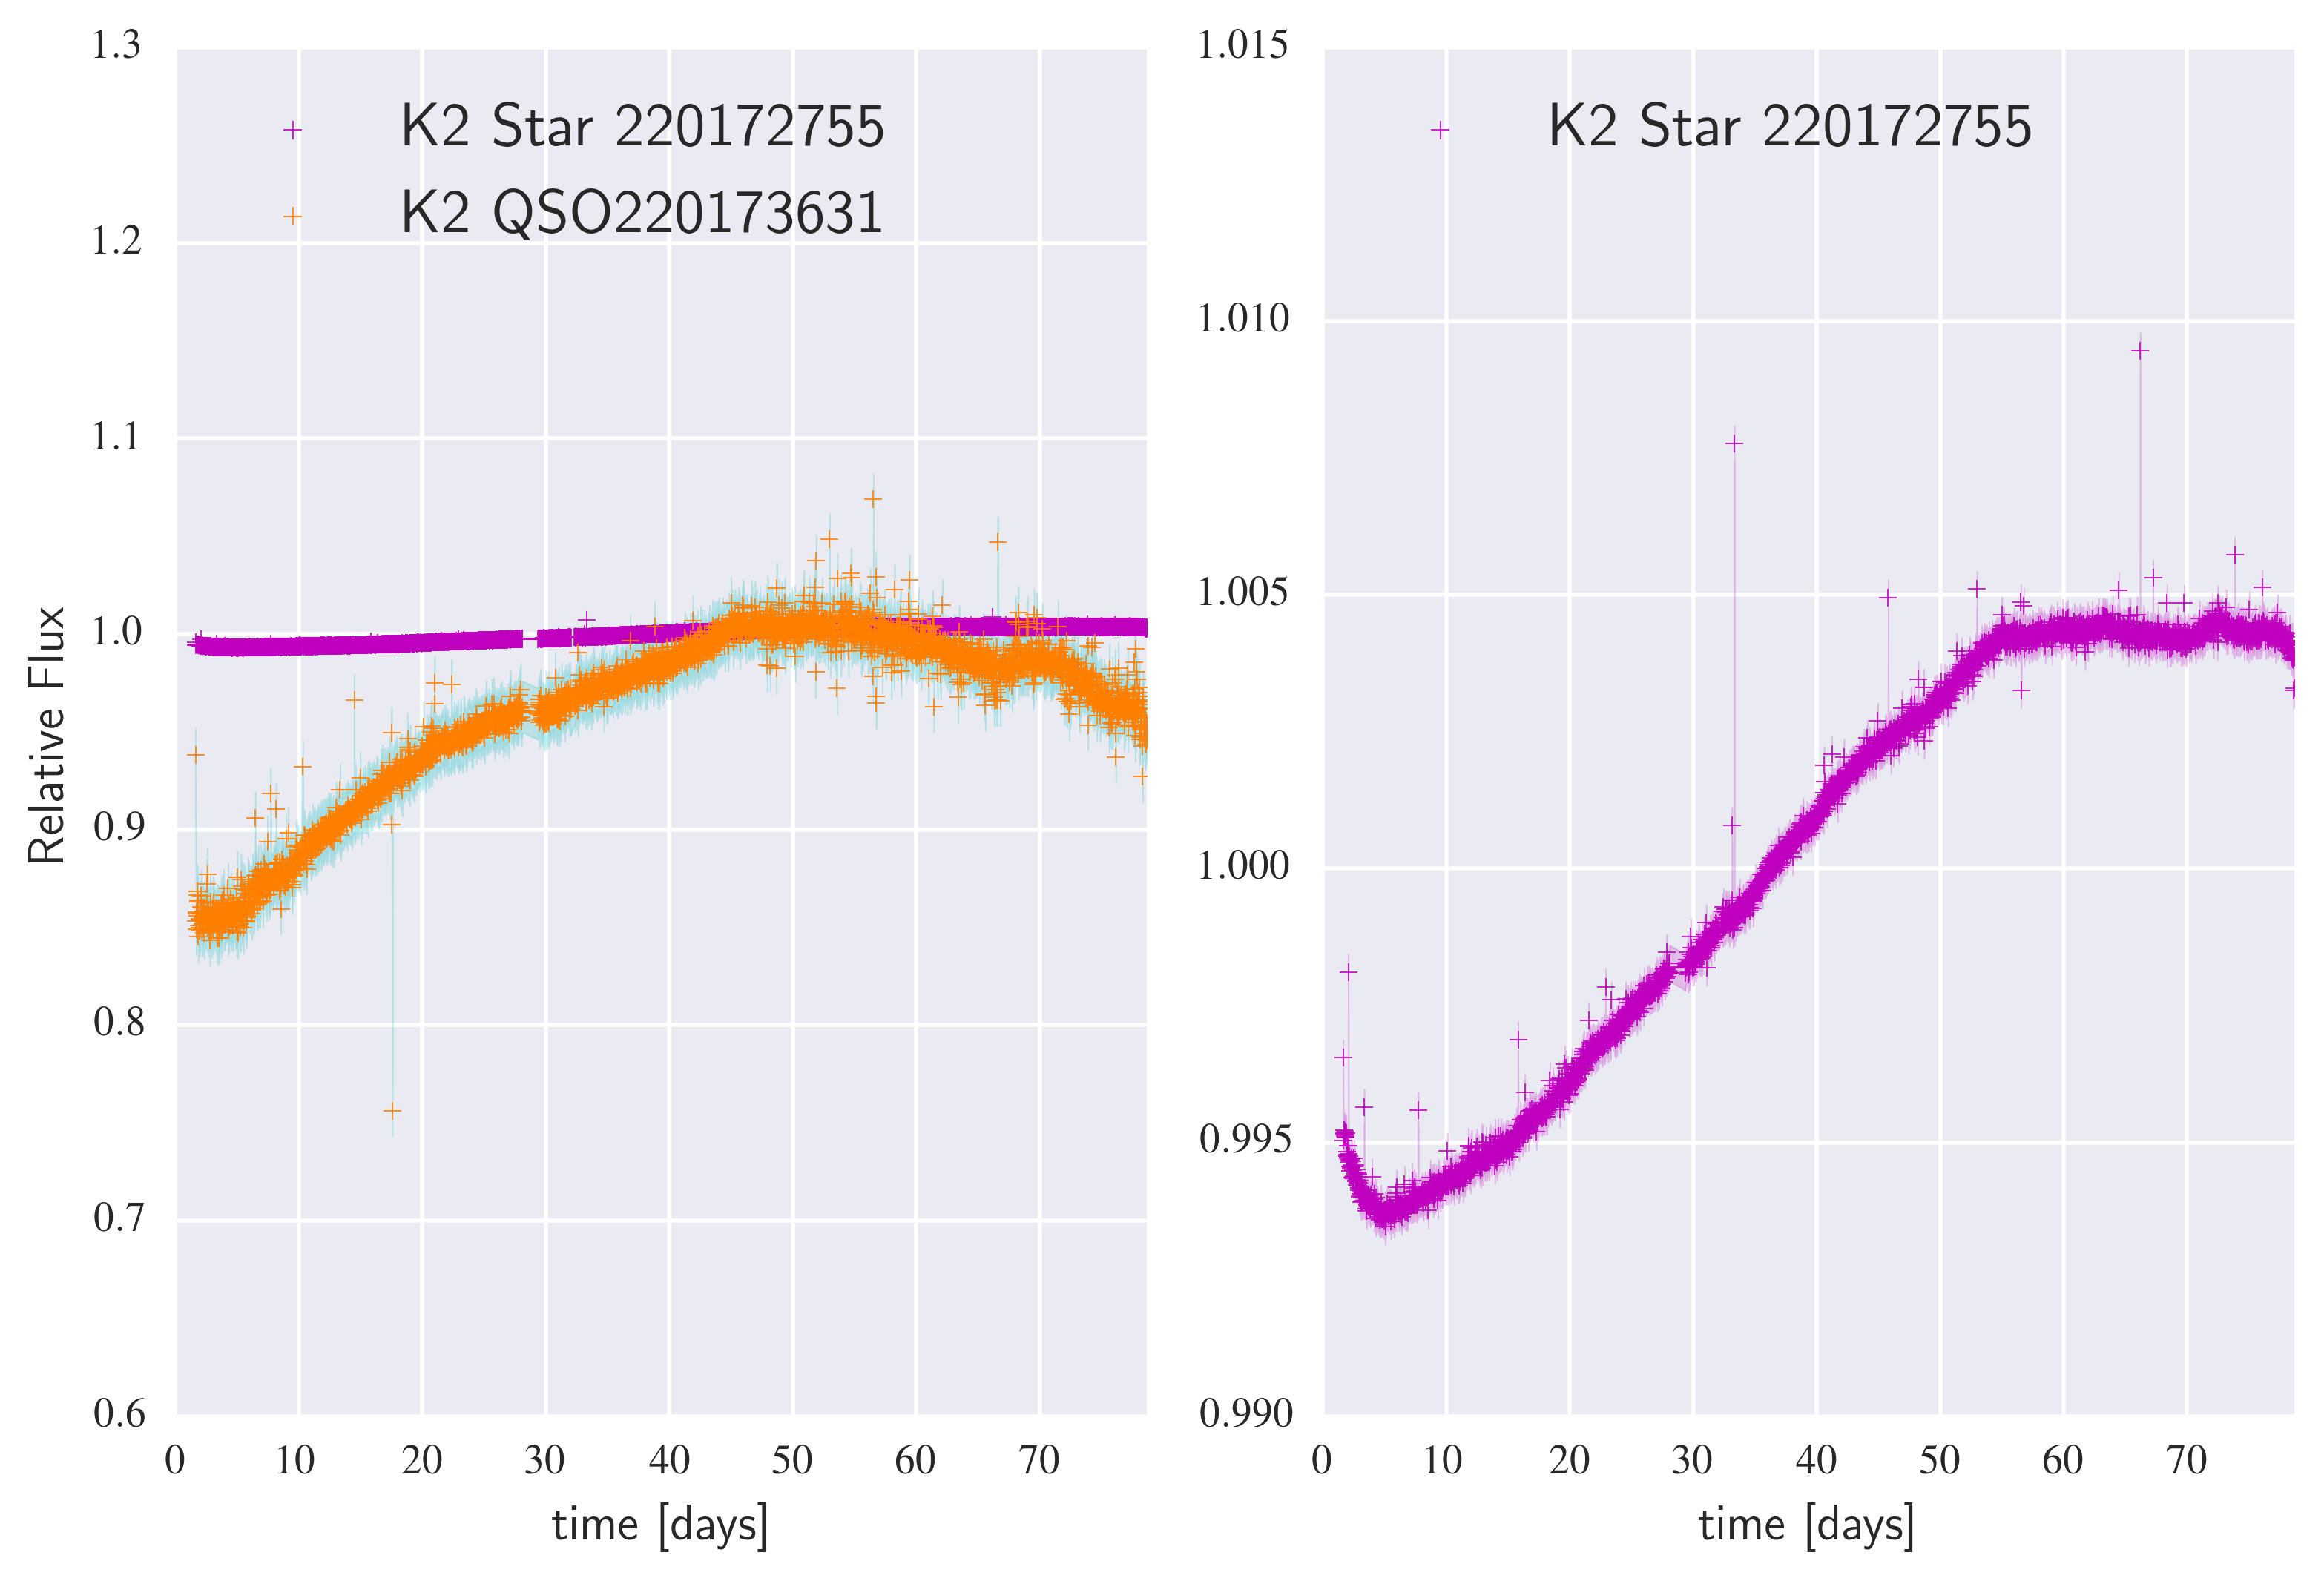
\includegraphics[width=\columnwidth]{220173631NearestNeighbor.png}
 	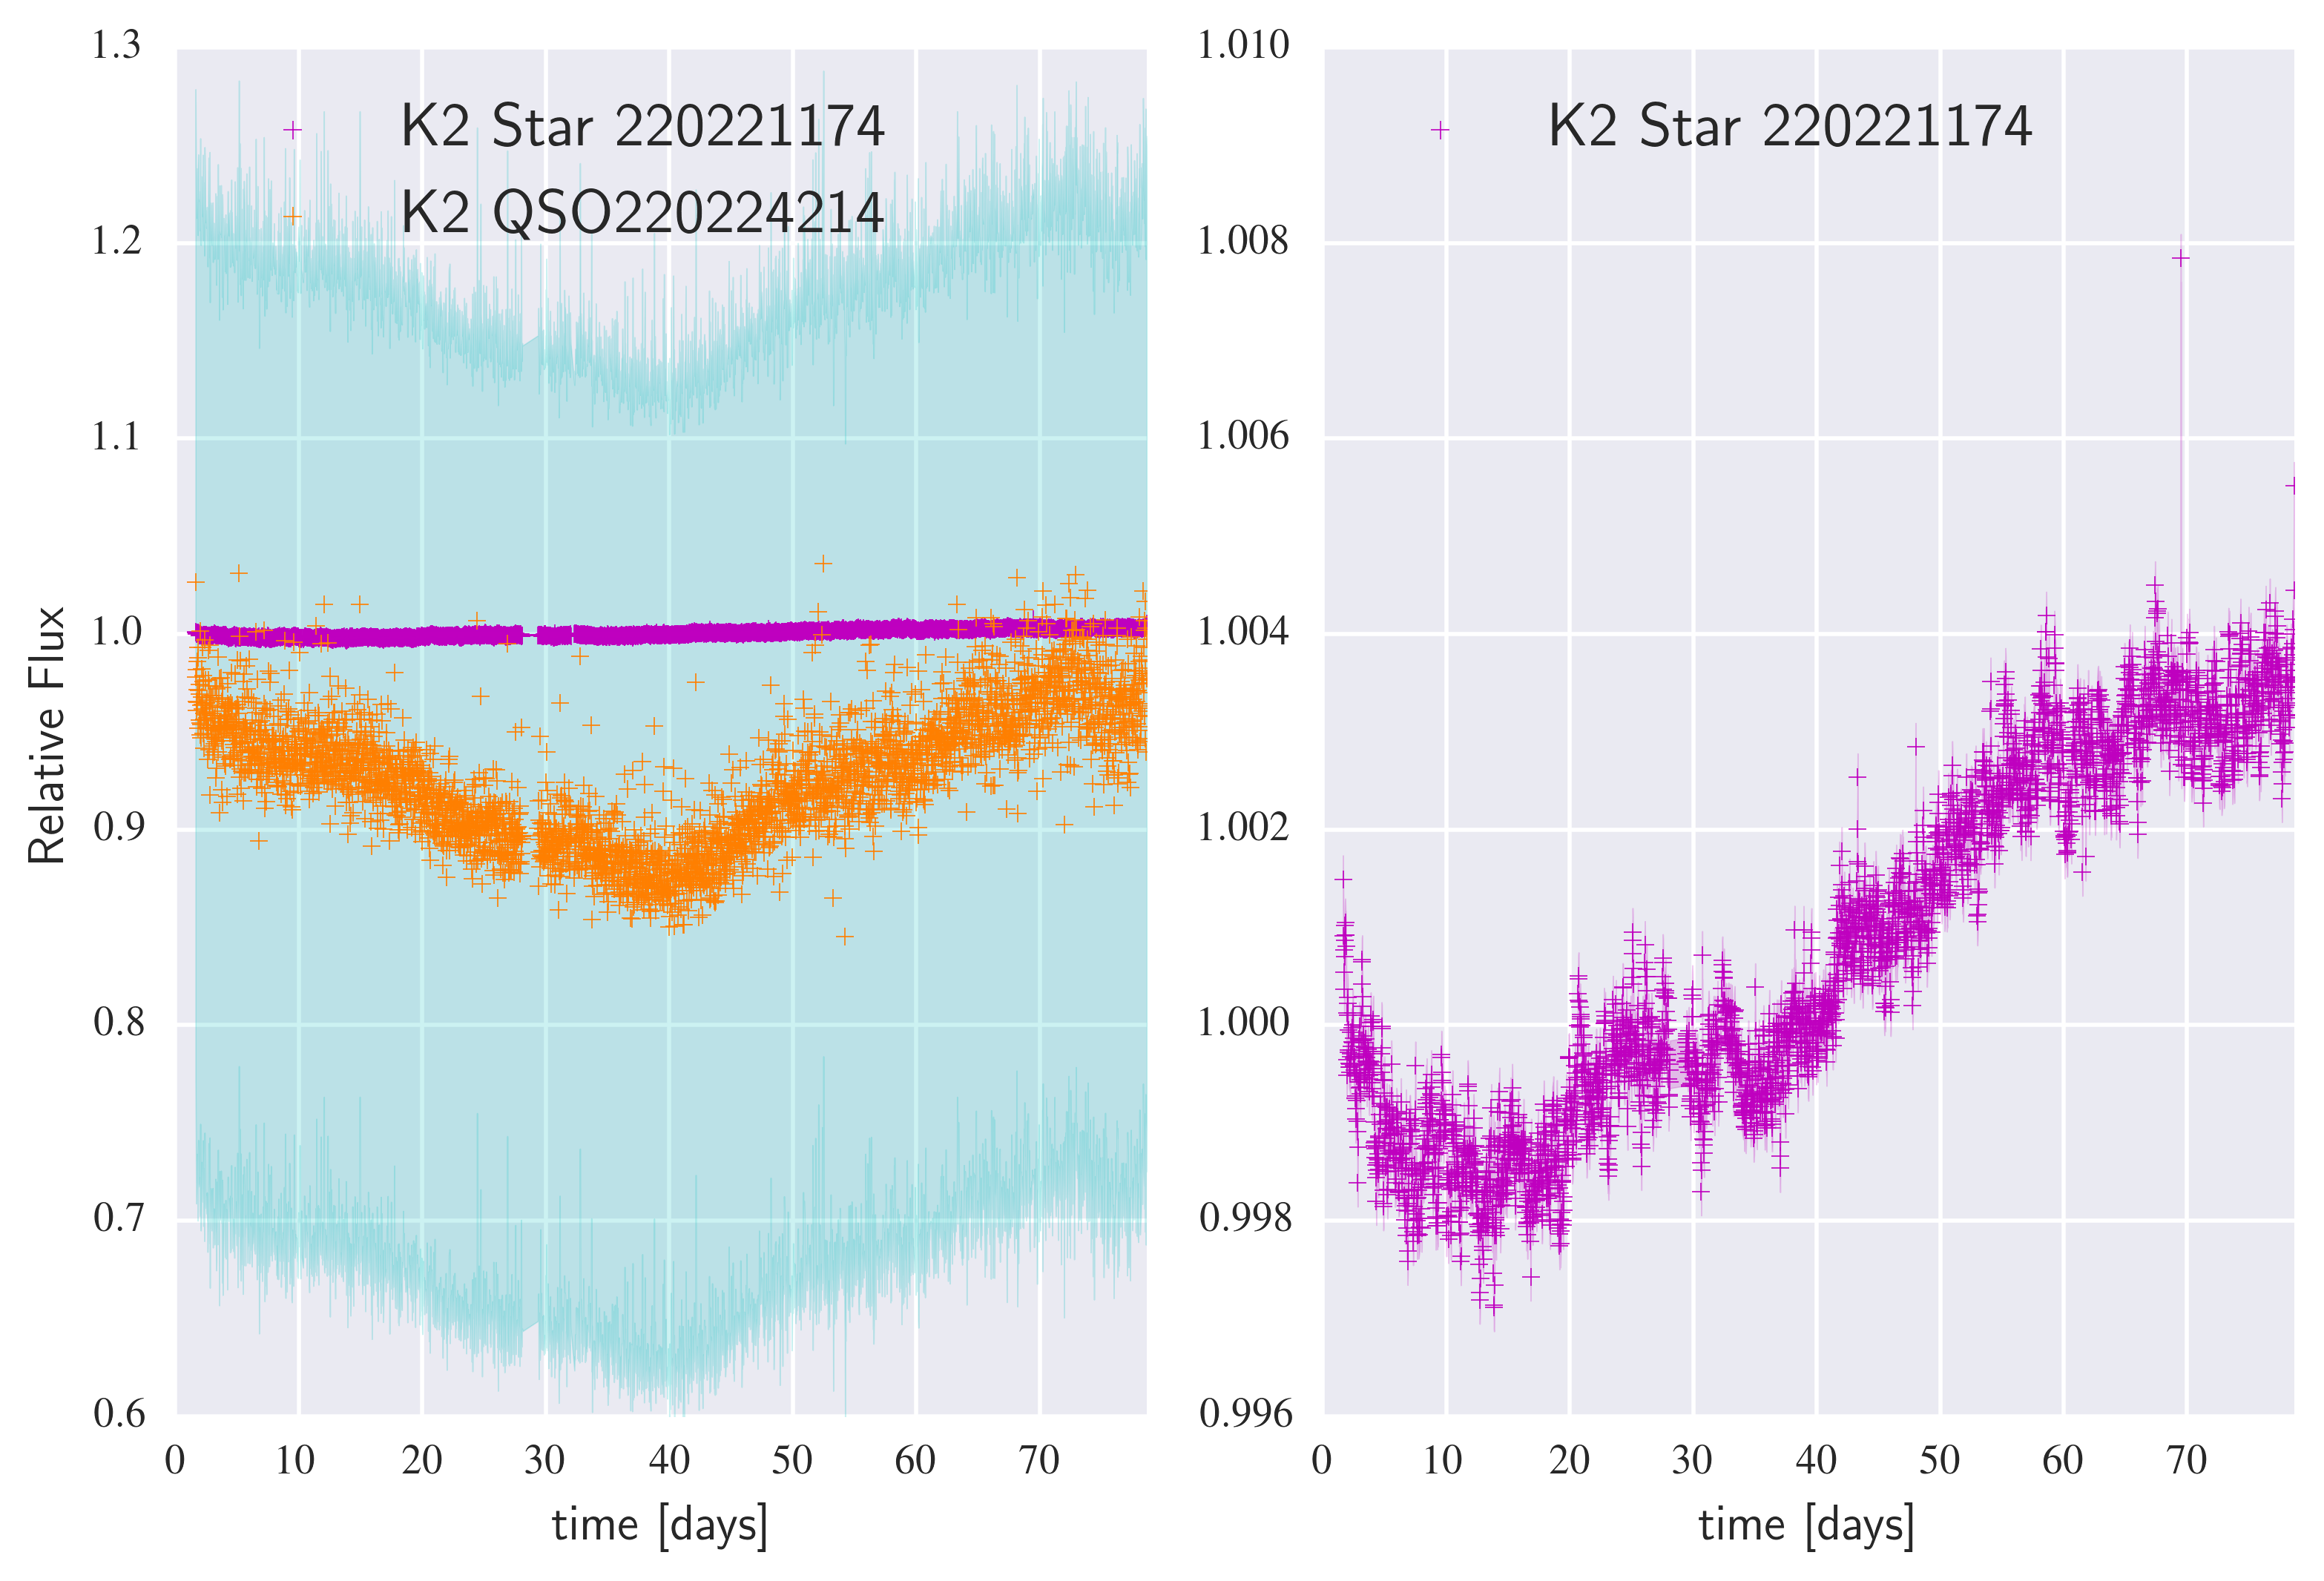
\includegraphics[width=\columnwidth]{220224214NearestNeighbor.png}
 	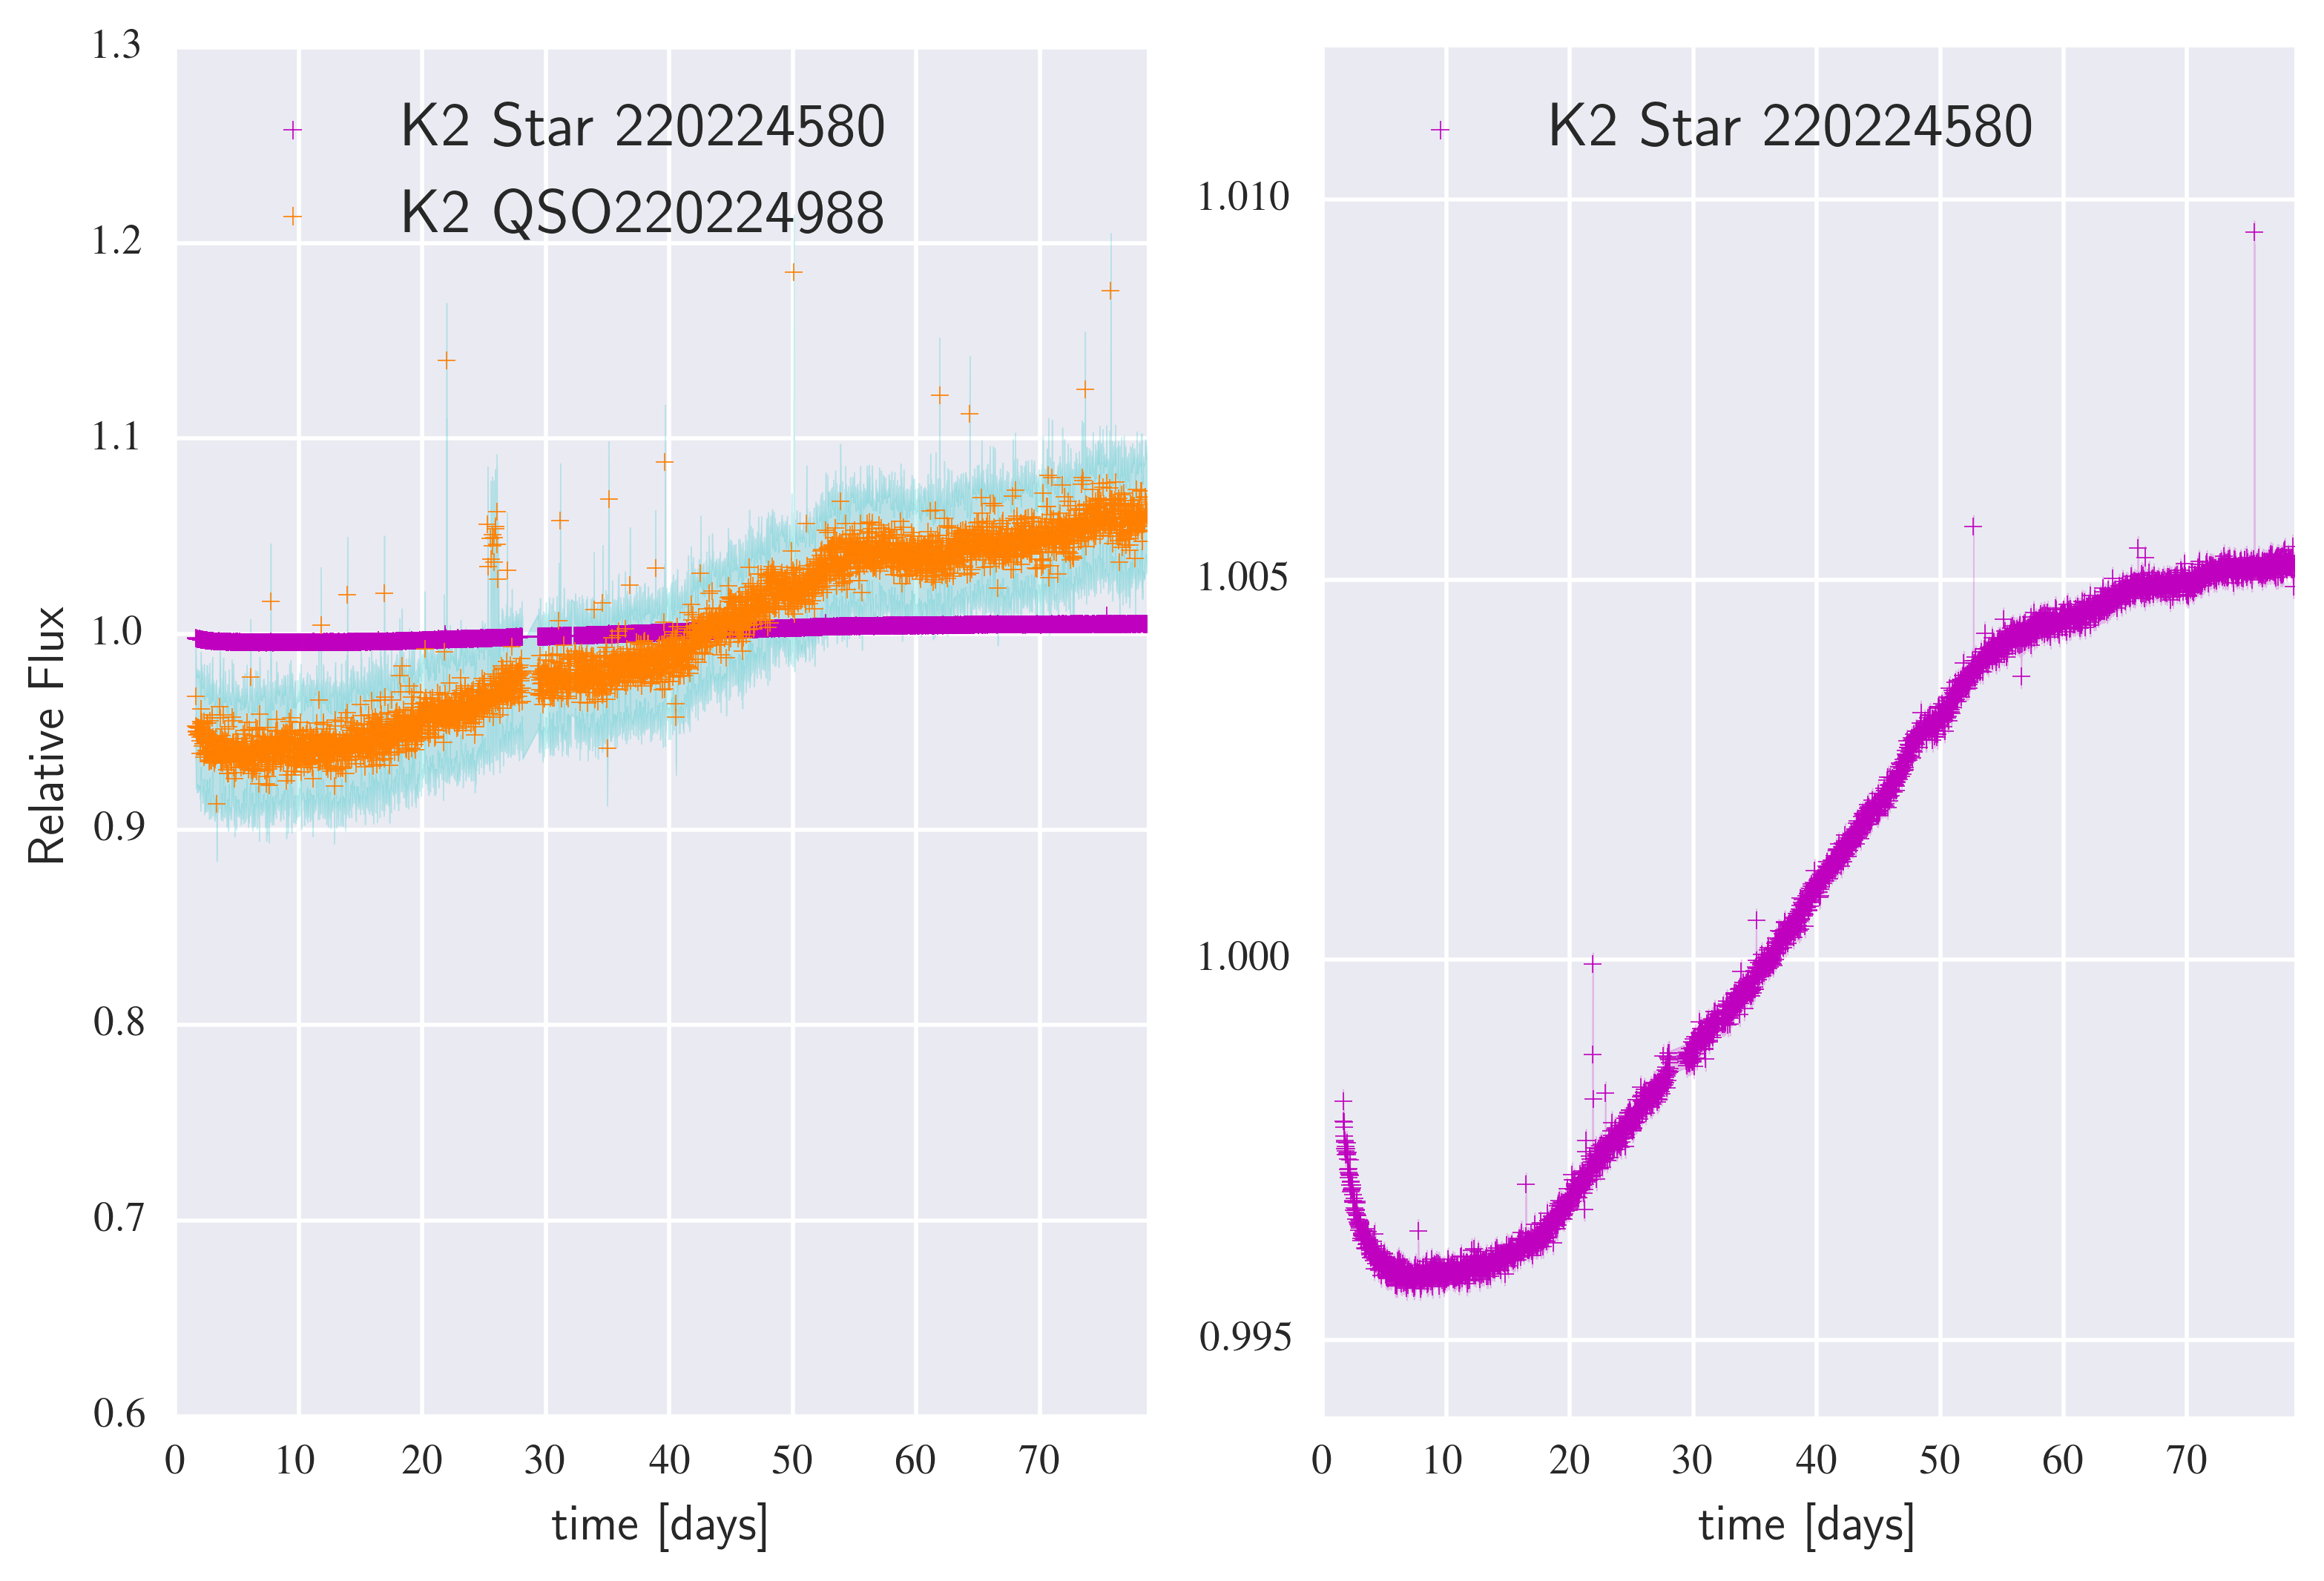
\includegraphics[width=\columnwidth]{220224988NearestNeighbor.png}
 	\caption{}
 	\label{fig:example_figure}
 \end{figure}
 
 
 
  \begin{figure}
  	% To include a figure from a file named example.*
  	% Allowable file formats are eps or ps if compiling using latex
  	% or pdf, png, jpg if compiling using pdflatex
 	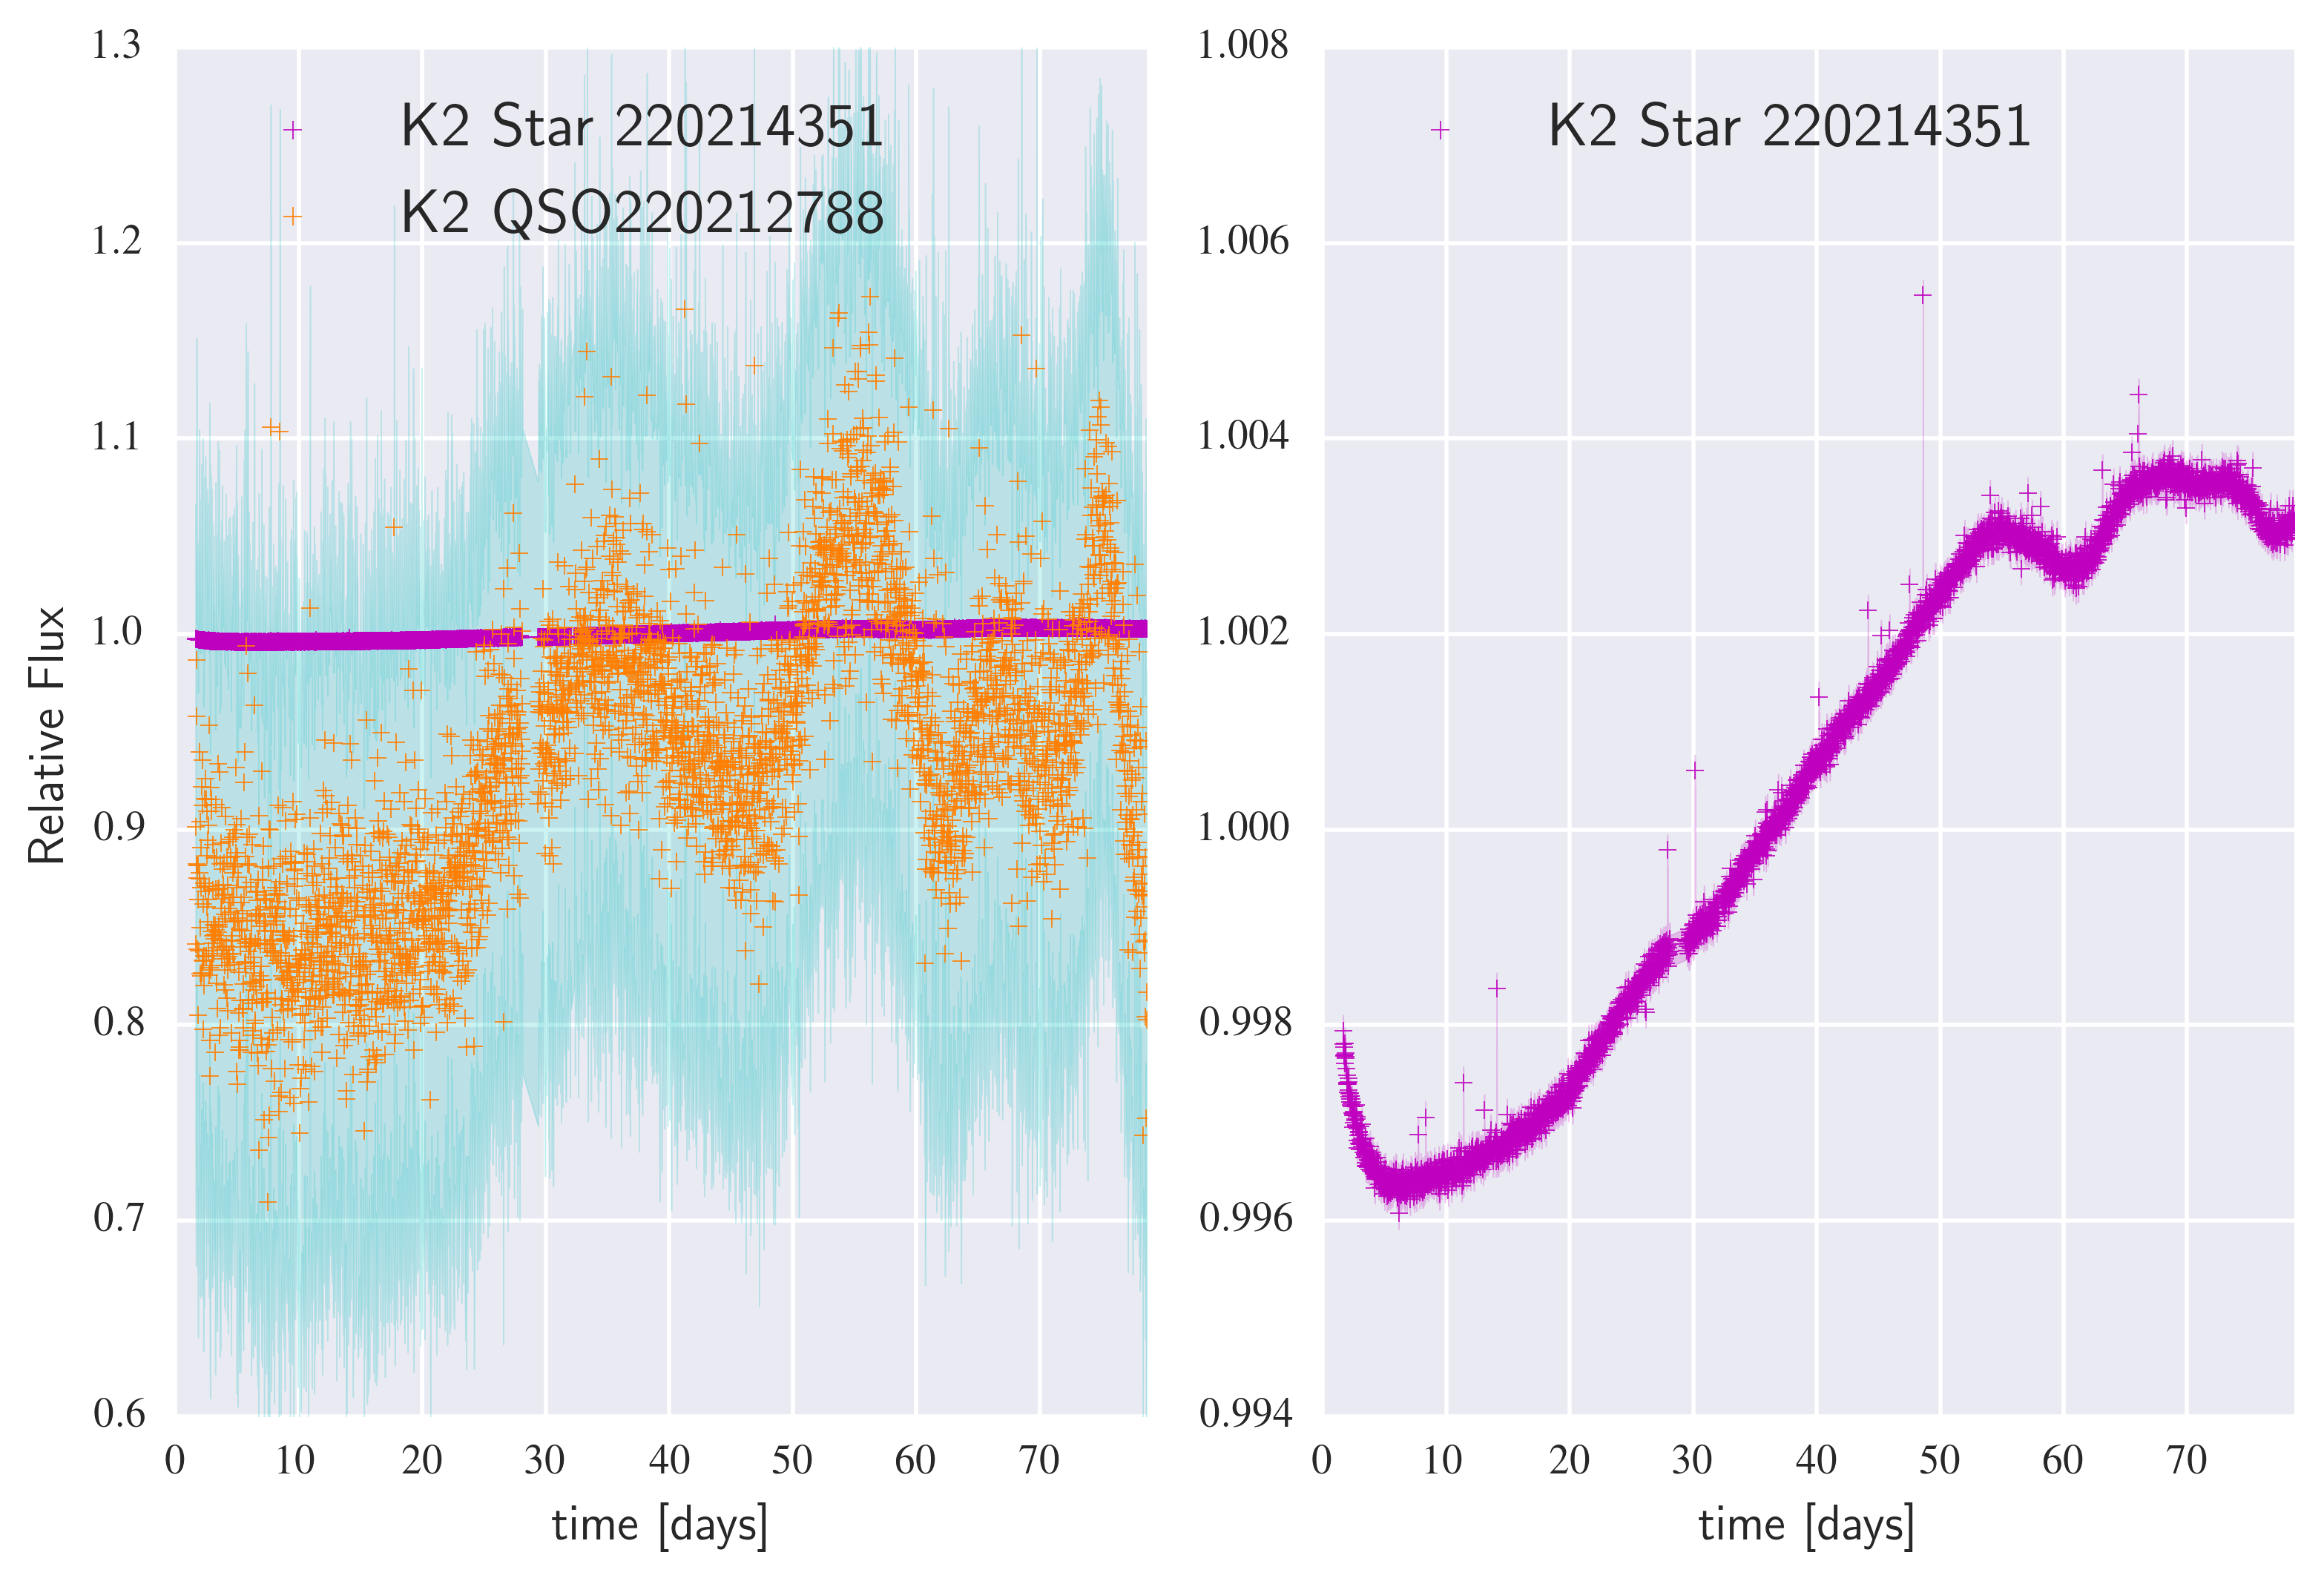
\includegraphics[width=\columnwidth]{220212788NearestNeighbor.png}
 	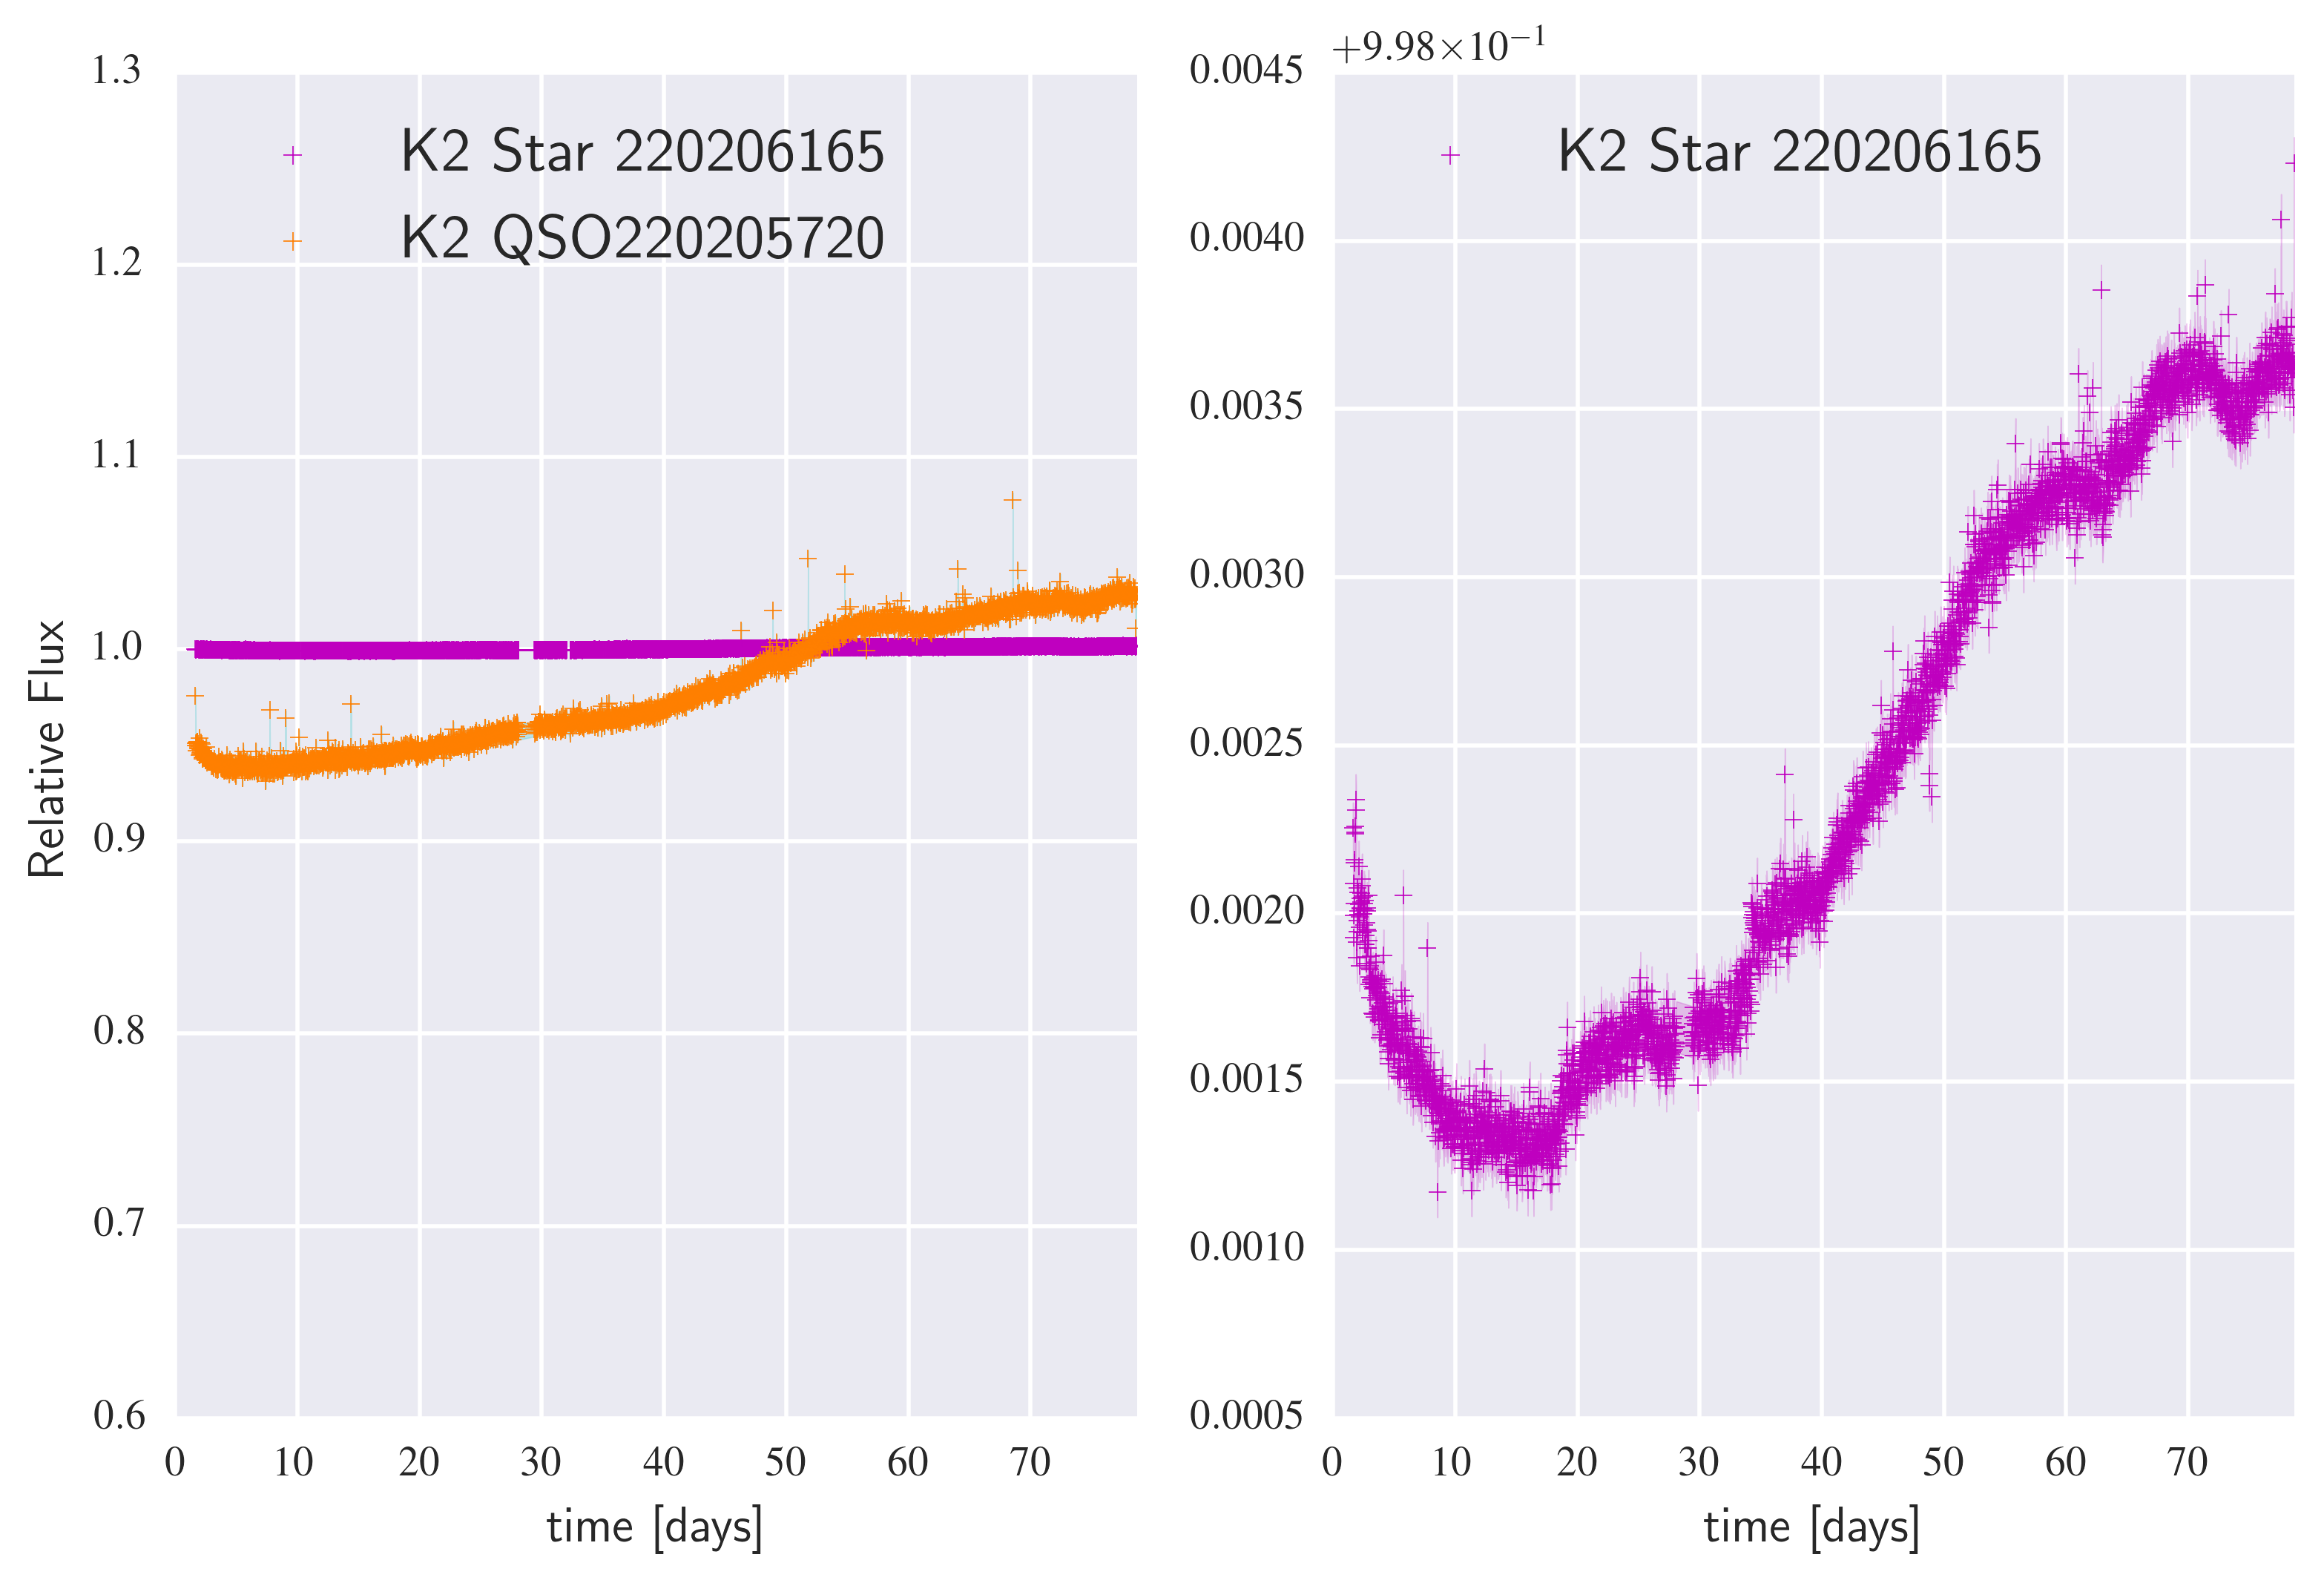
\includegraphics[width=\columnwidth]{220205720NearestNeighbor.png}
 	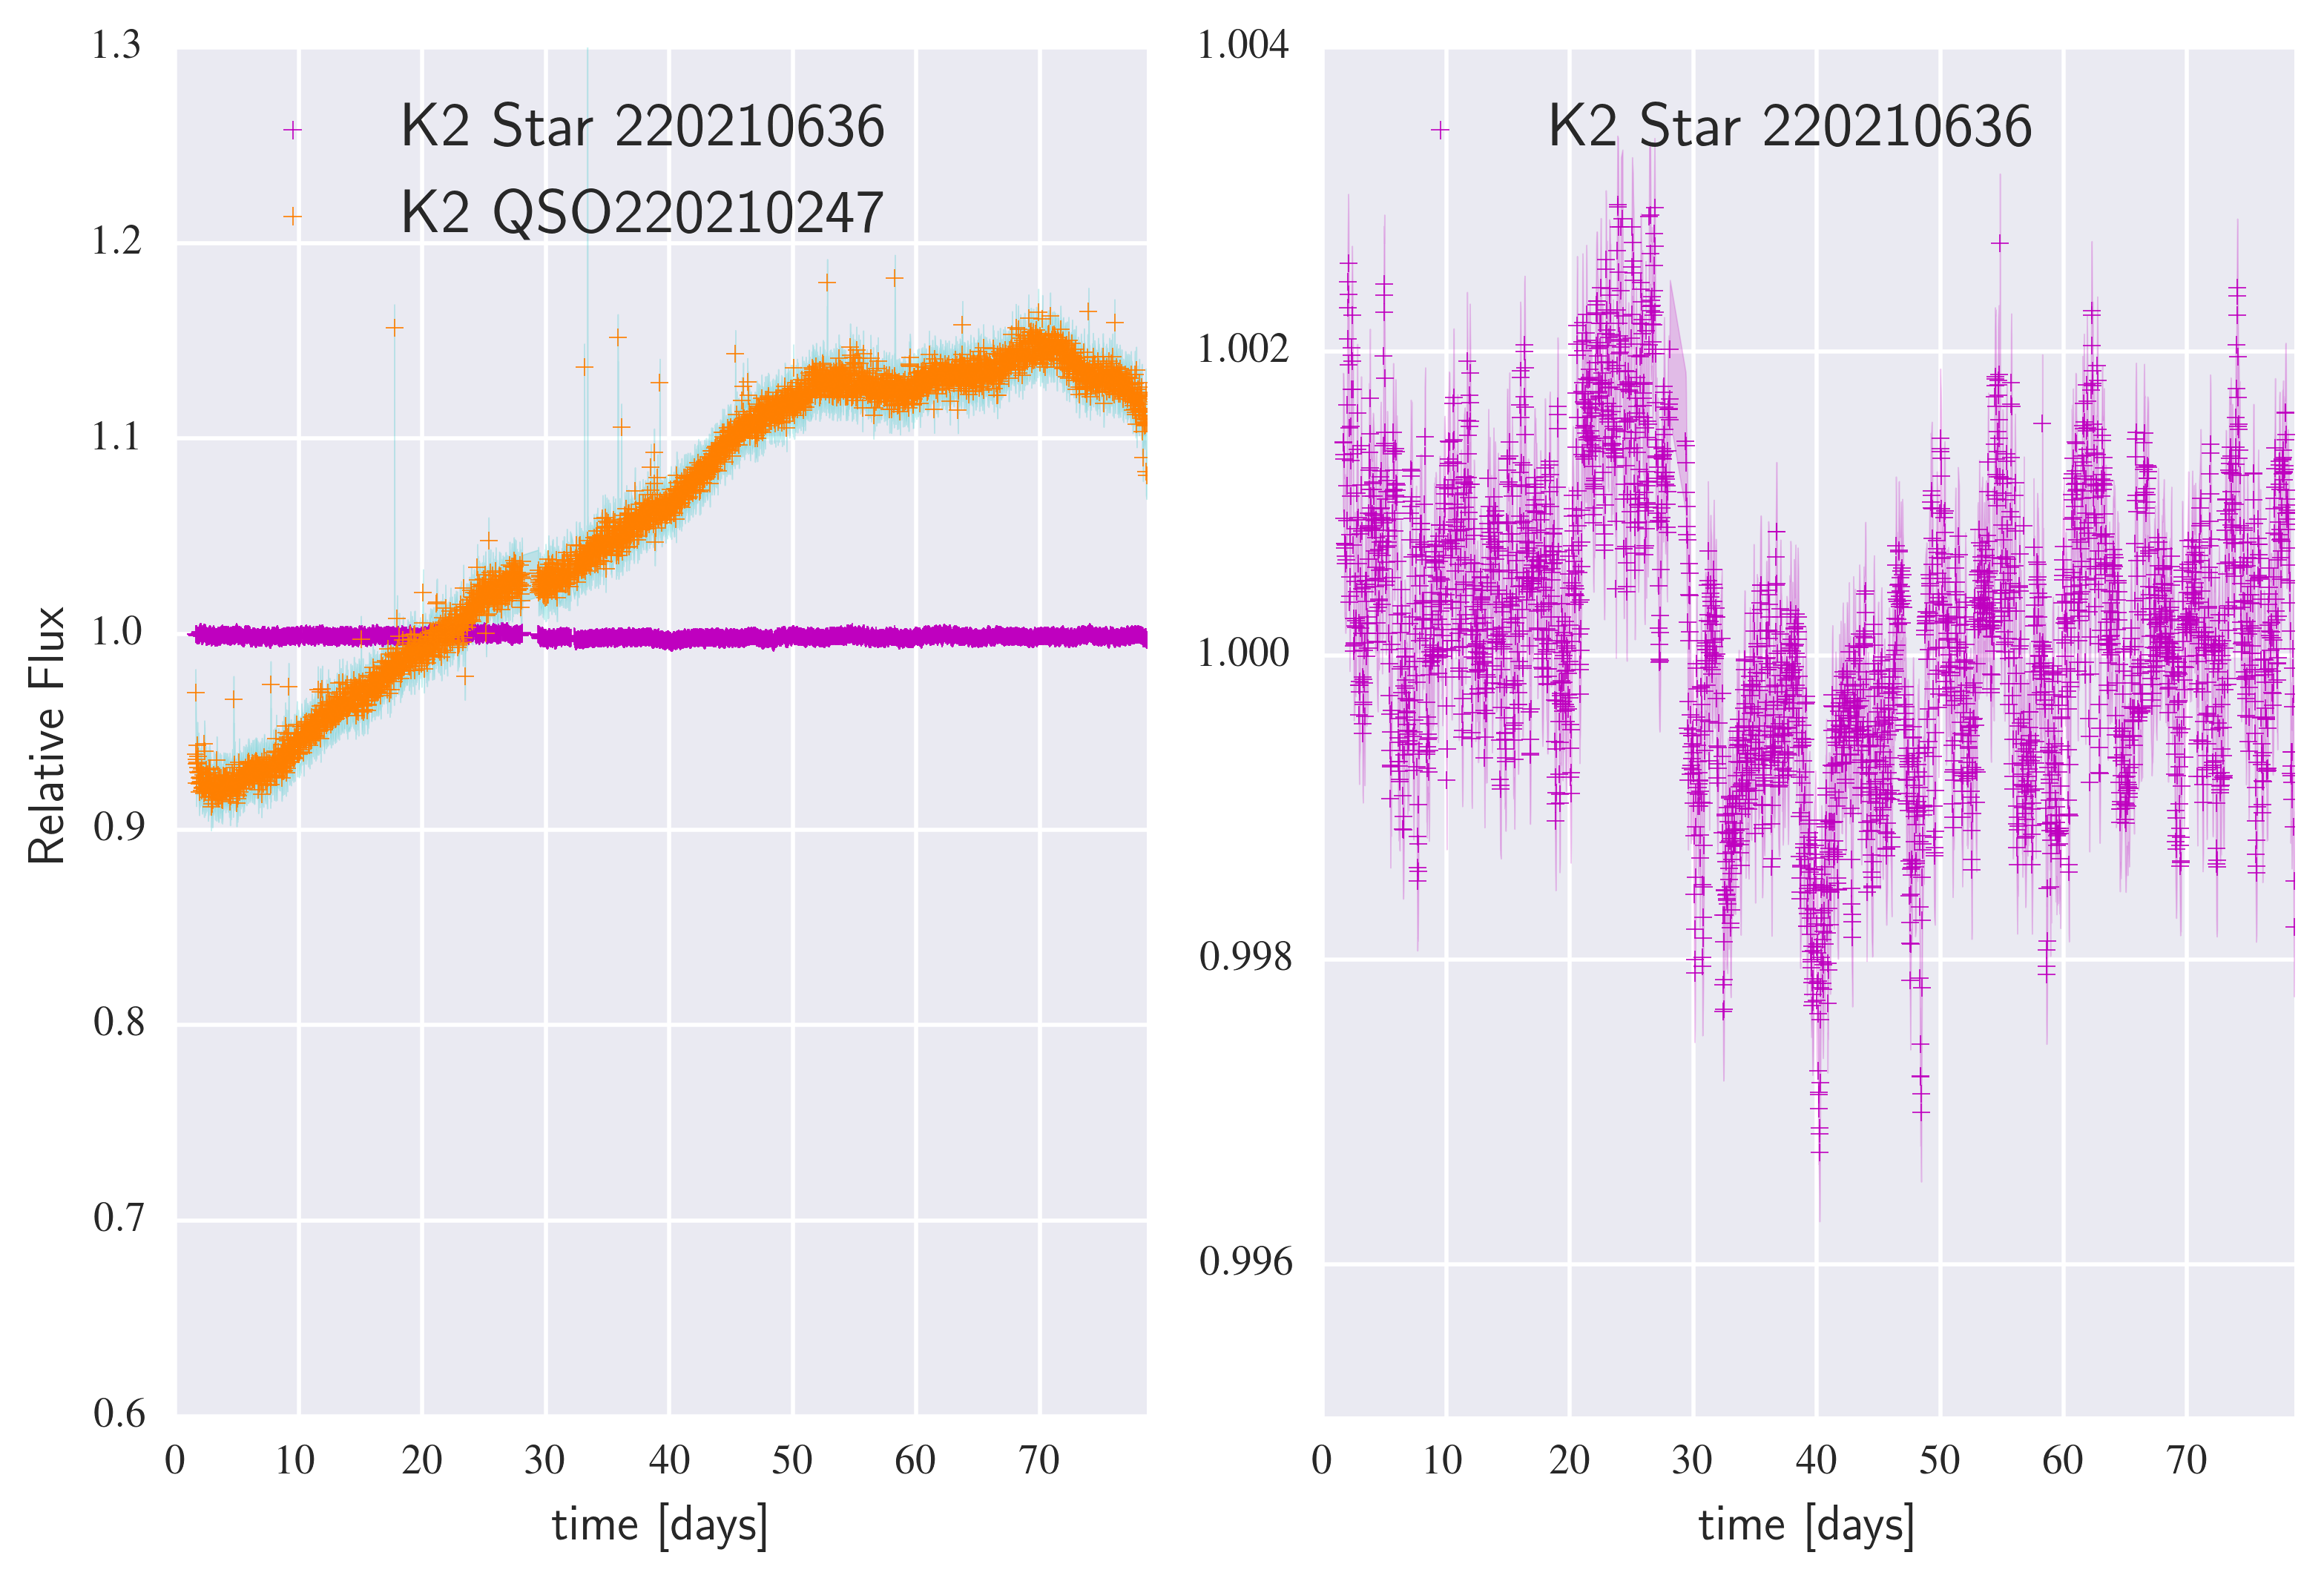
\includegraphics[width=\columnwidth]{220210247NearestNeighbor.png}
  	\caption{}
  	\label{fig:example_figure}
  \end{figure}
  
  
   \begin{figure}
   	% To include a figure from a file named example.*
   	% Allowable file formats are eps or ps if compiling using latex
   	% or pdf, png, jpg if compiling using pdflatex
 	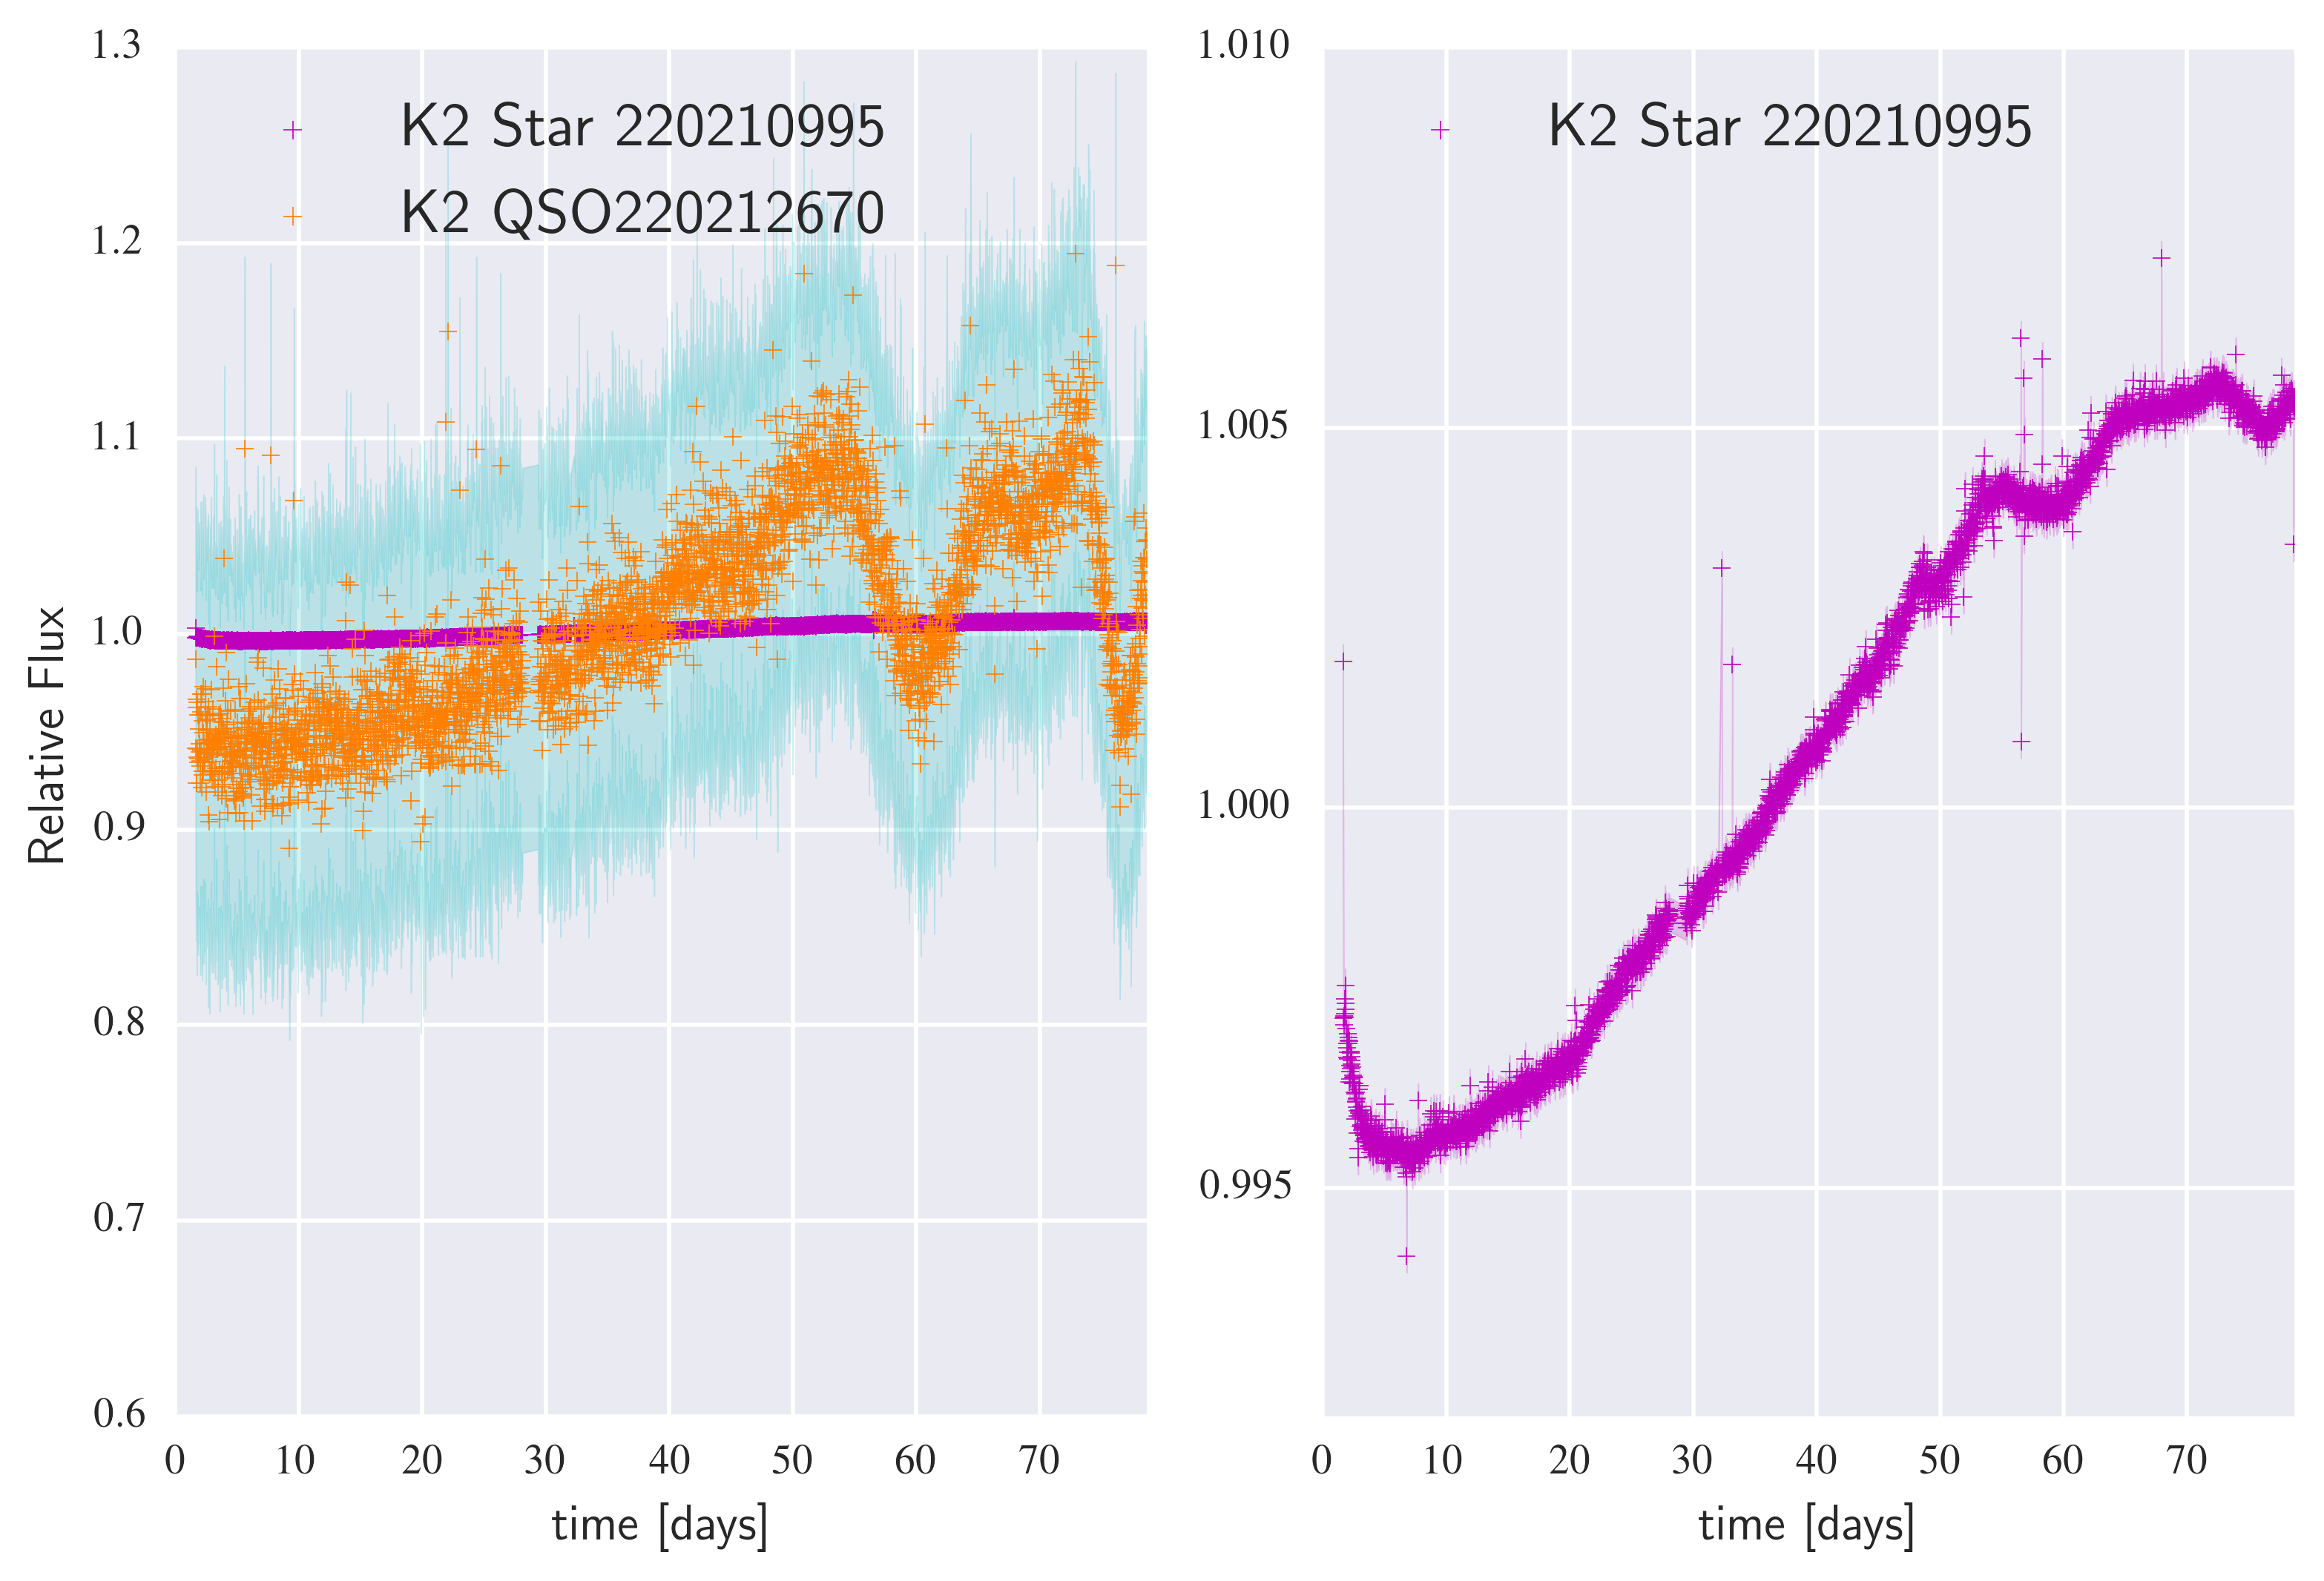
\includegraphics[width=\columnwidth]{220212670NearestNeighbor.png}
 	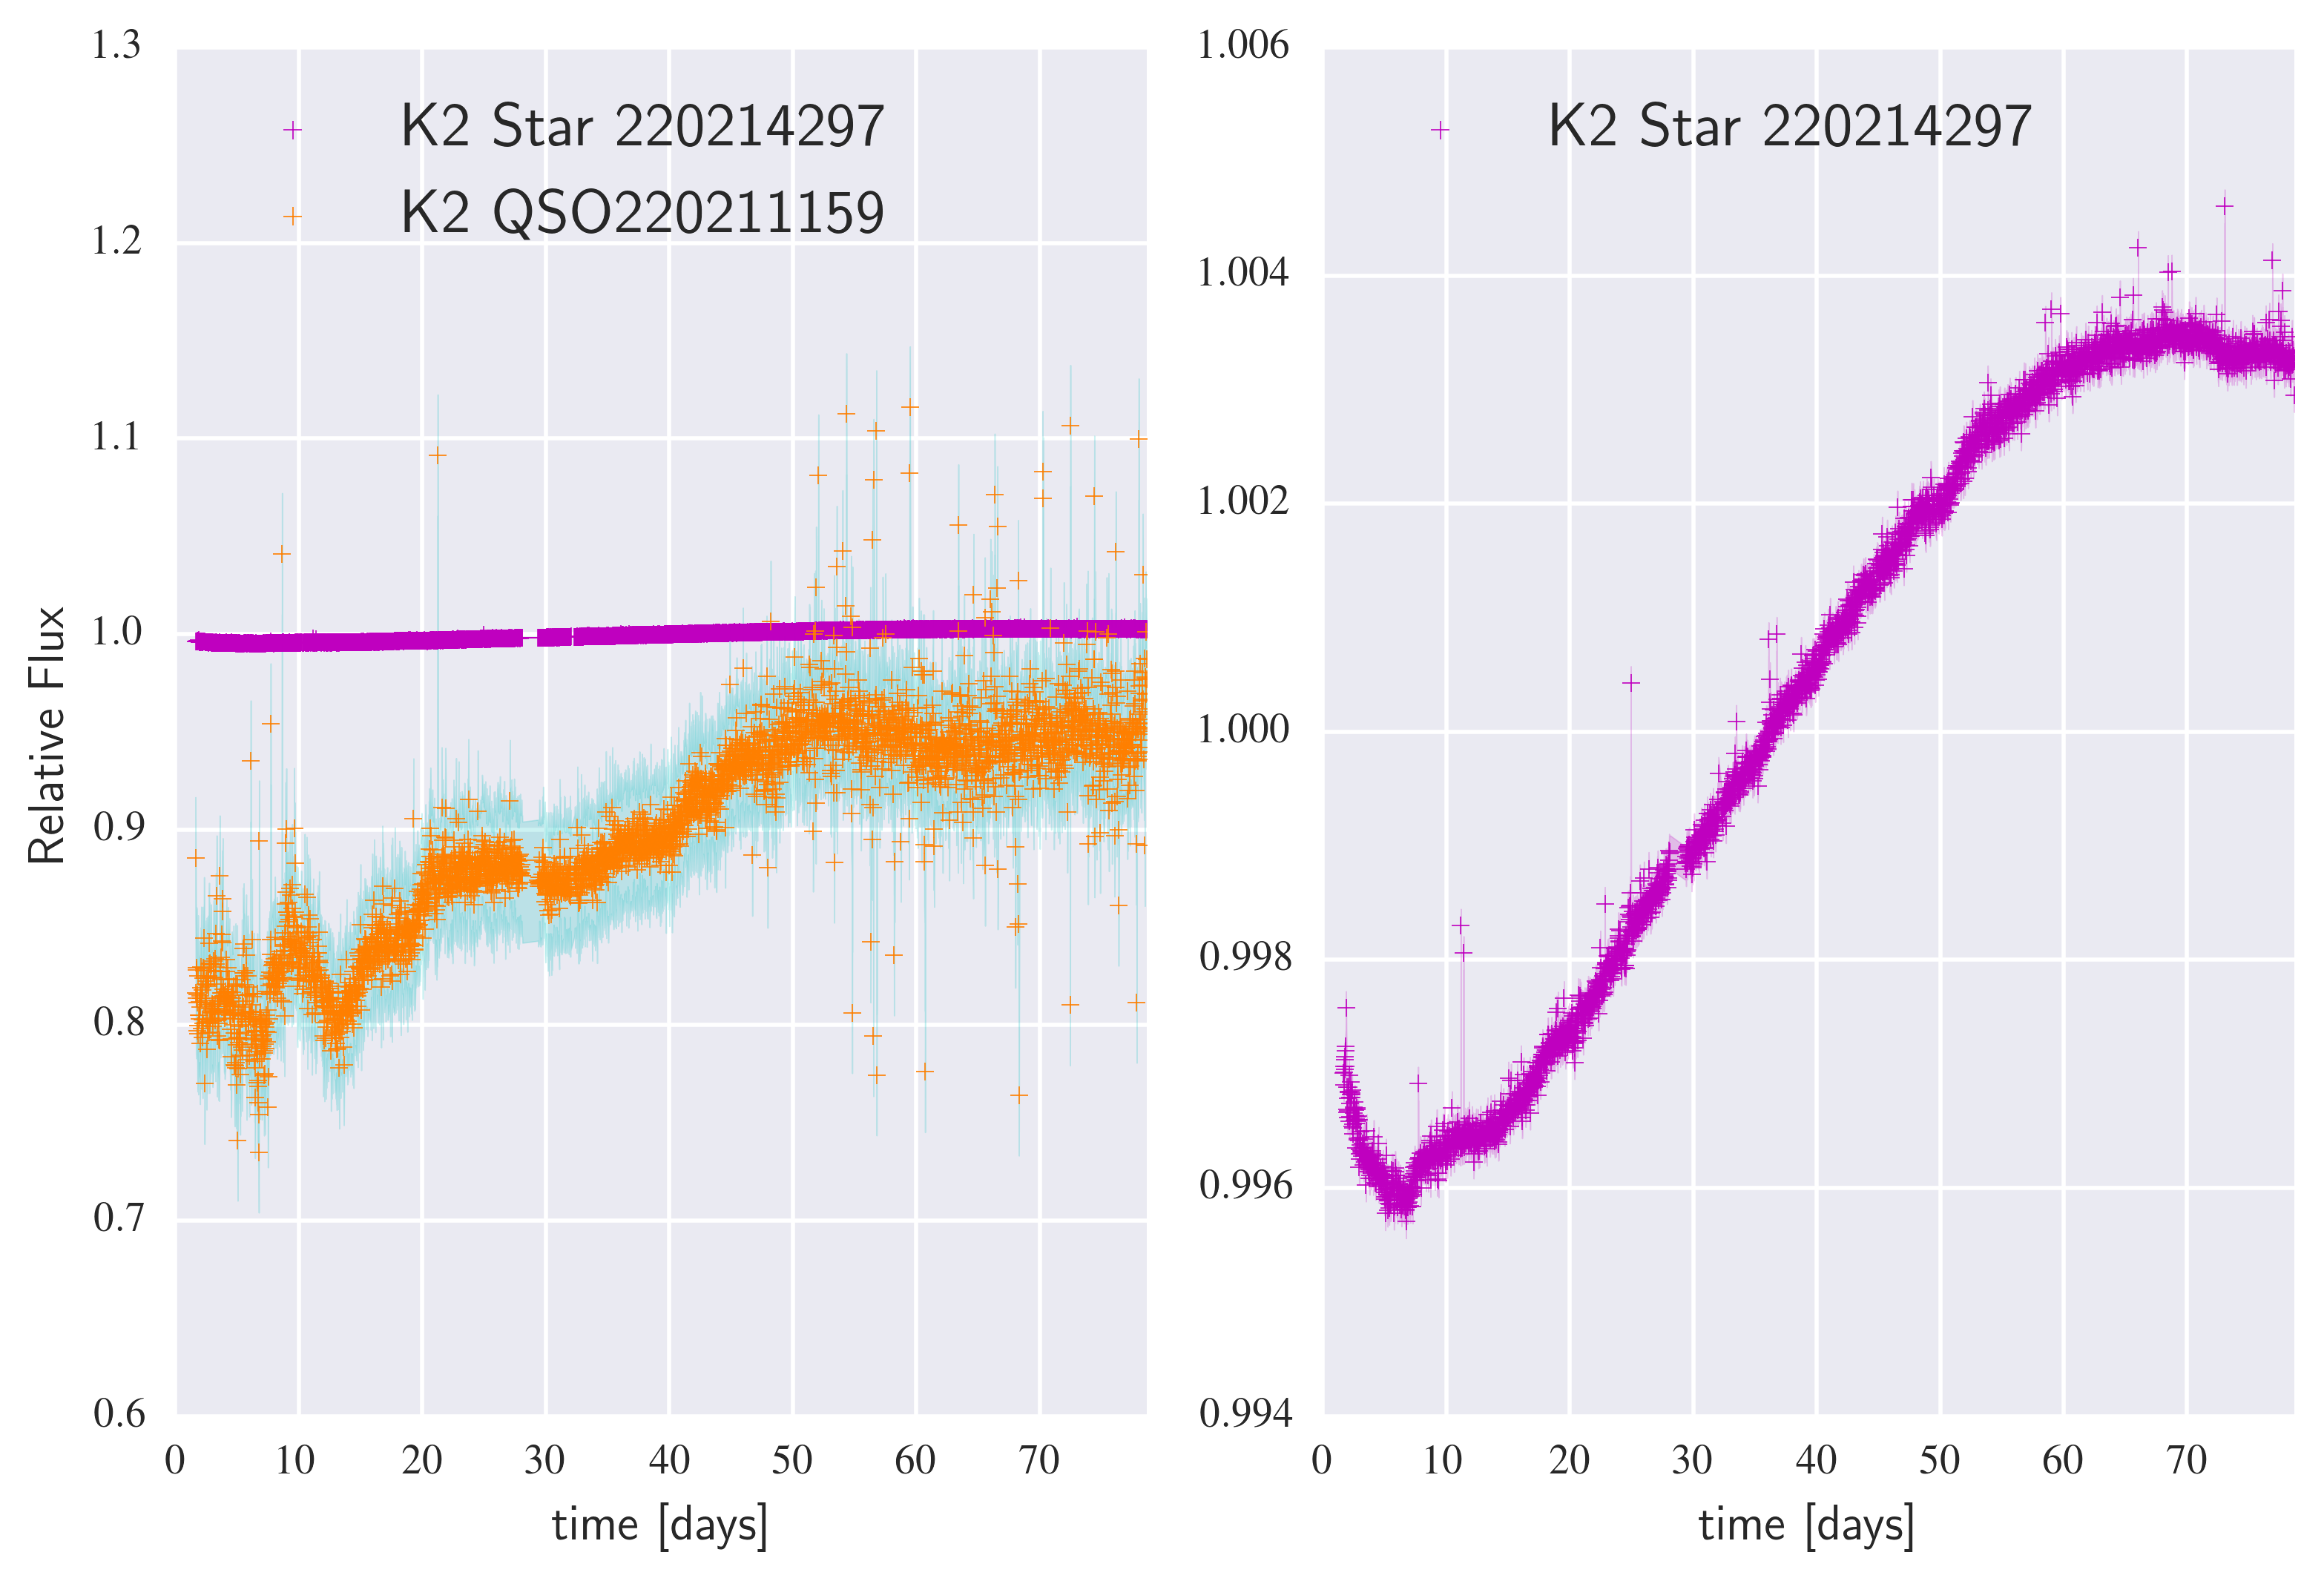
\includegraphics[width=\columnwidth]{220211159NearestNeighbor.png}
 	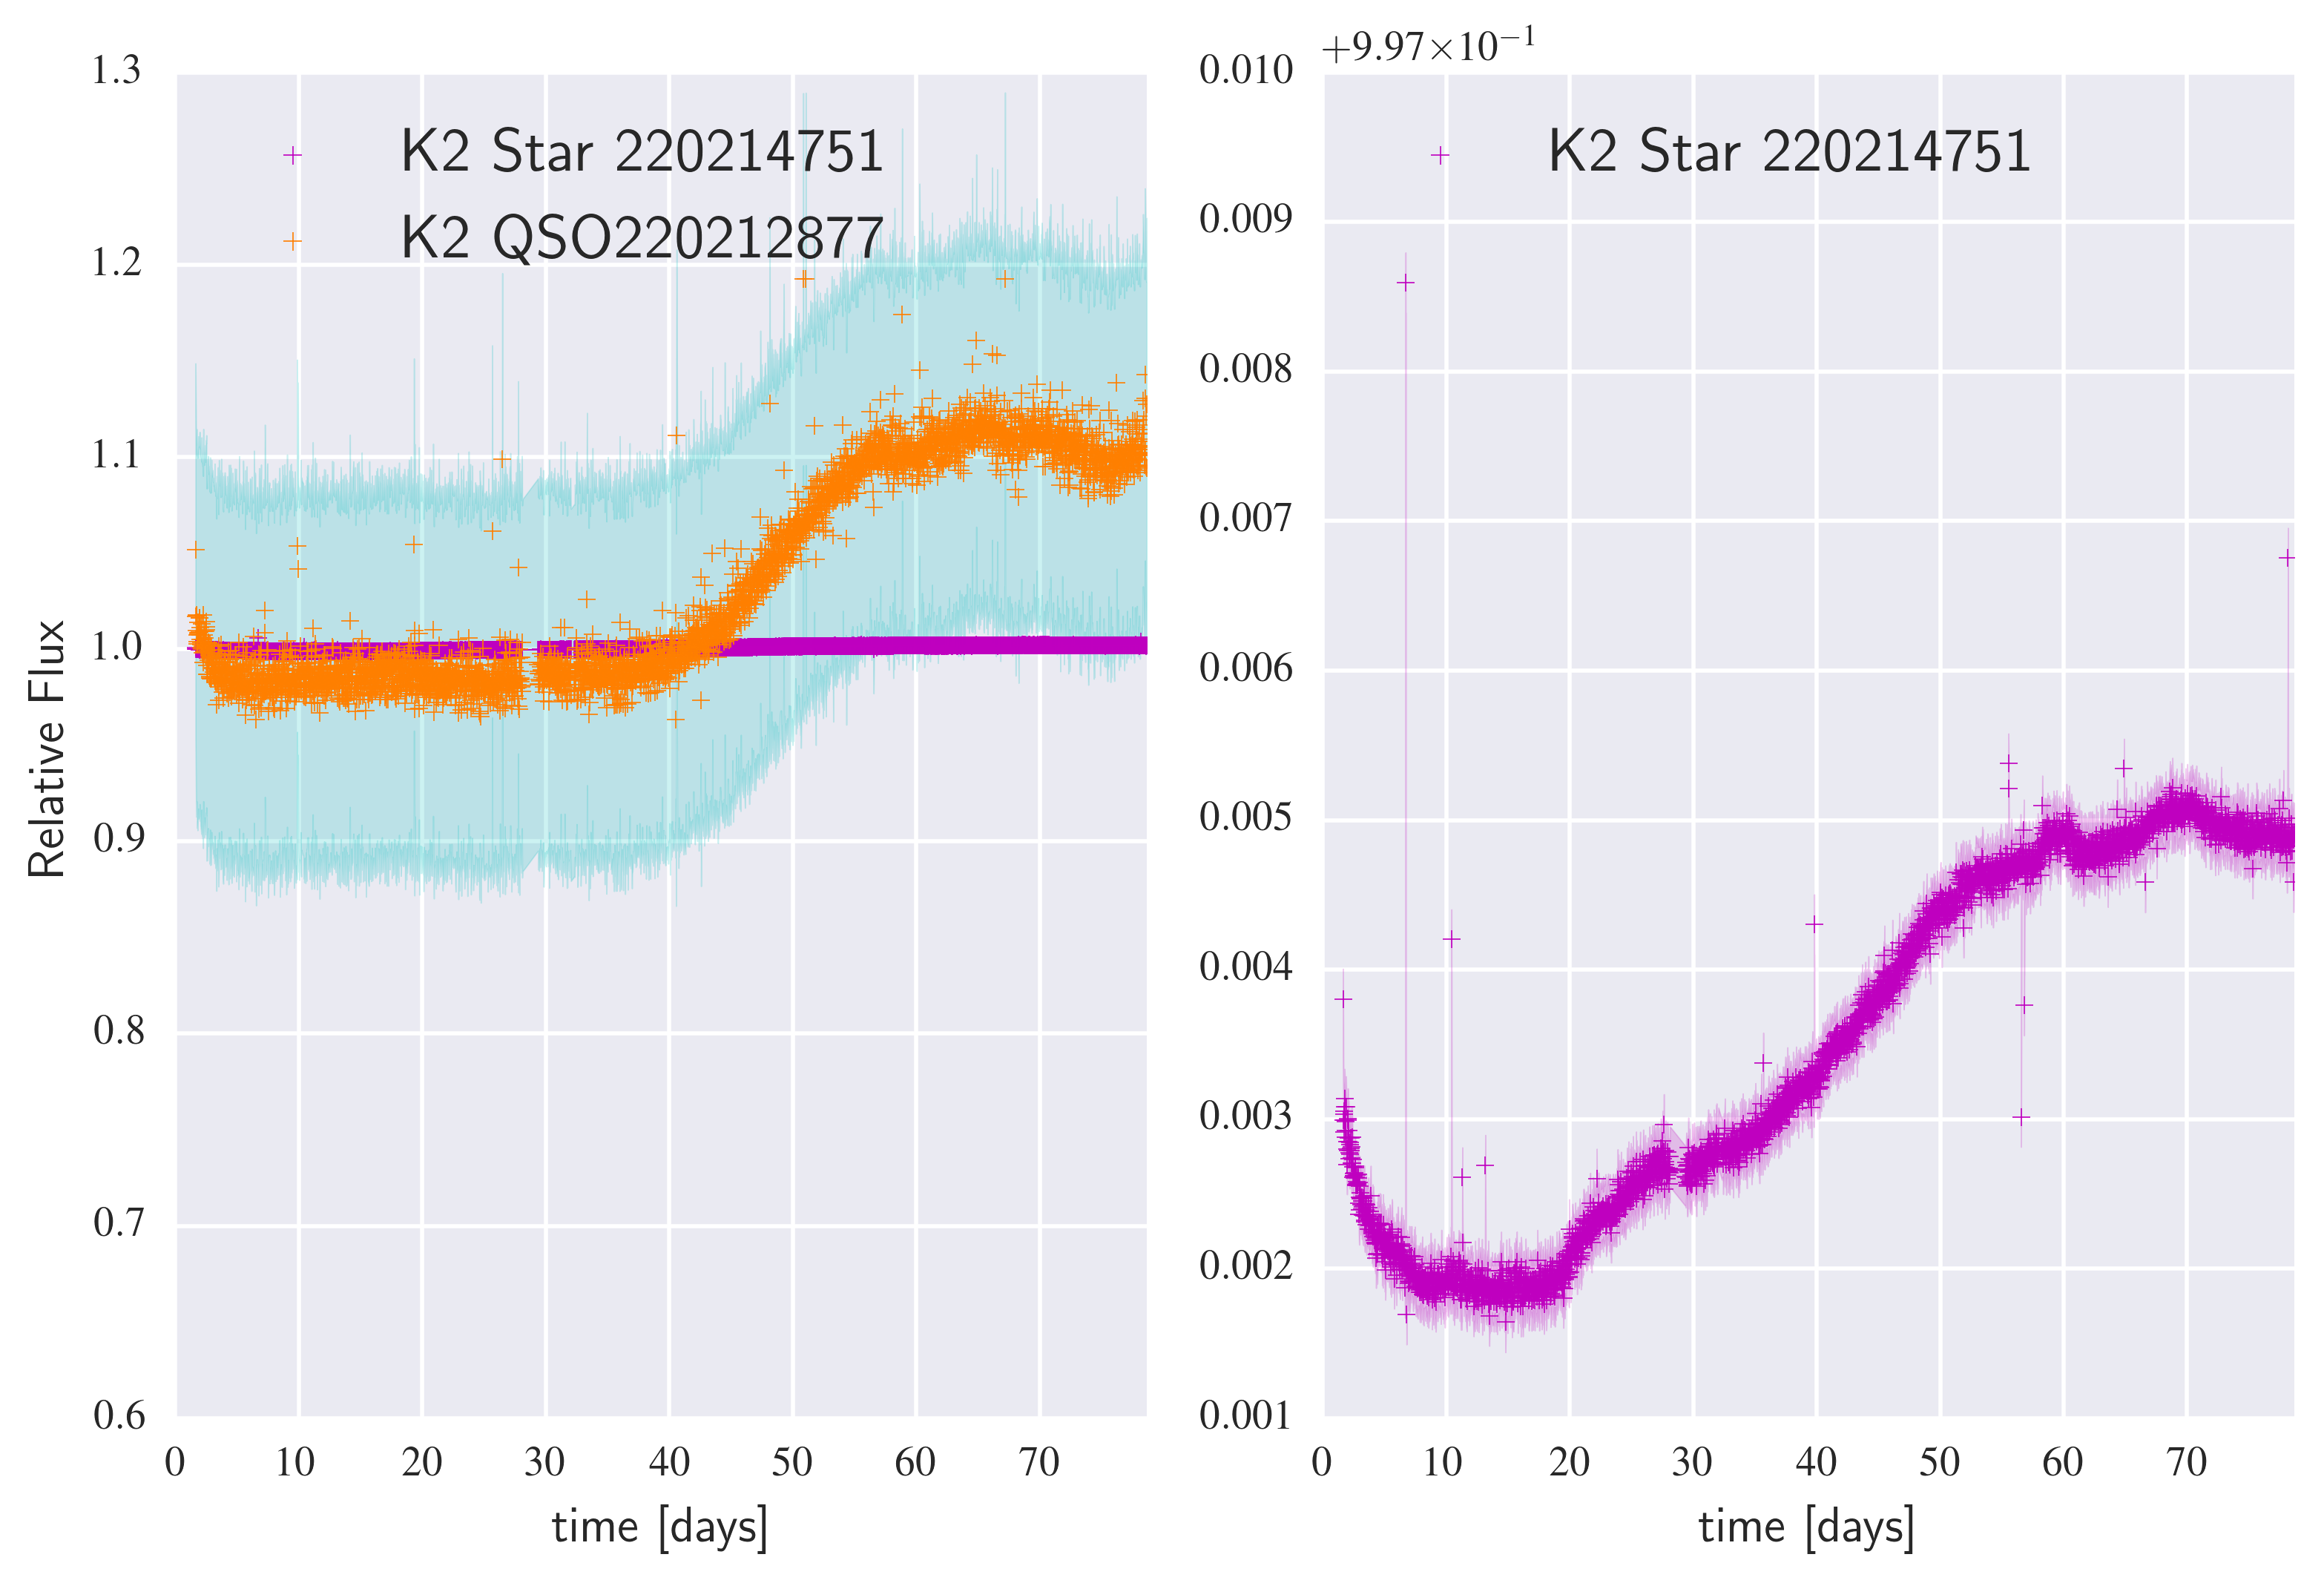
\includegraphics[width=\columnwidth]{220212877NearestNeighbor.png}
   	\caption{}
   	\label{fig:example_figure}
   \end{figure}
 
    \begin{figure}
    	% To include a figure from a file named example.*
    	% Allowable file formats are eps or ps if compiling using latex
    	% or pdf, png, jpg if compiling using pdflatex
 	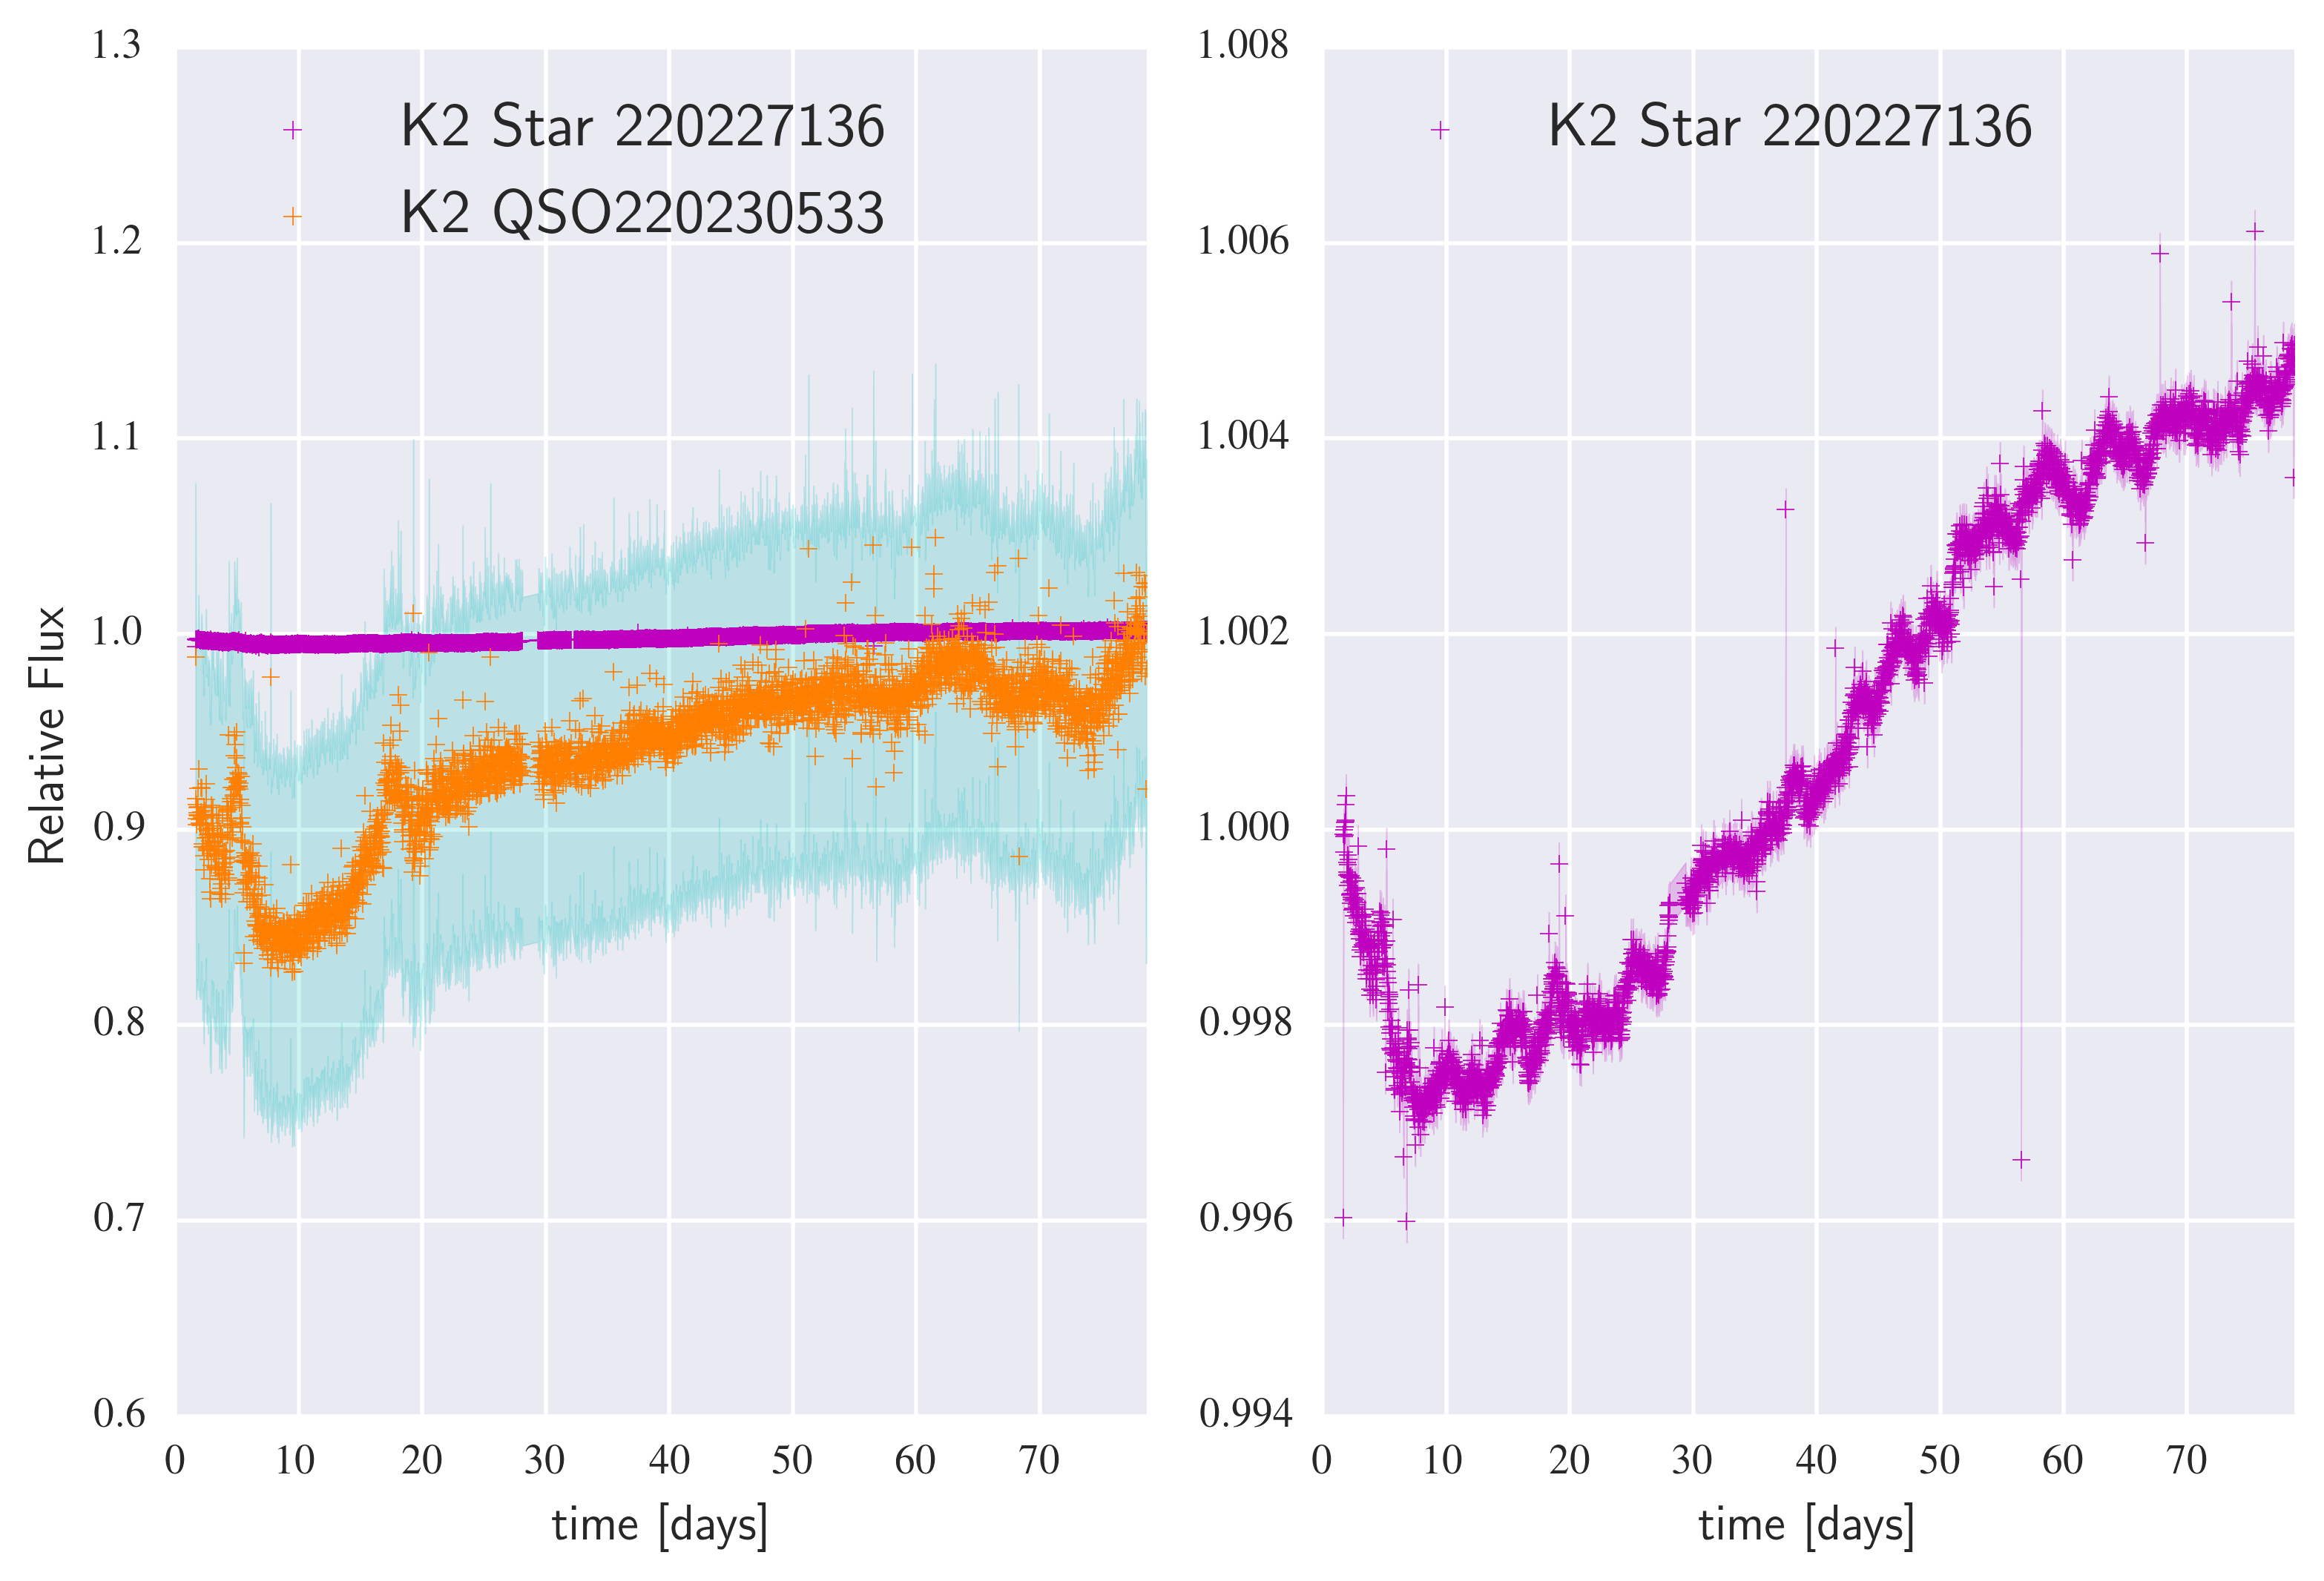
\includegraphics[width=\columnwidth]{220230533NearestNeighbor.png}
 	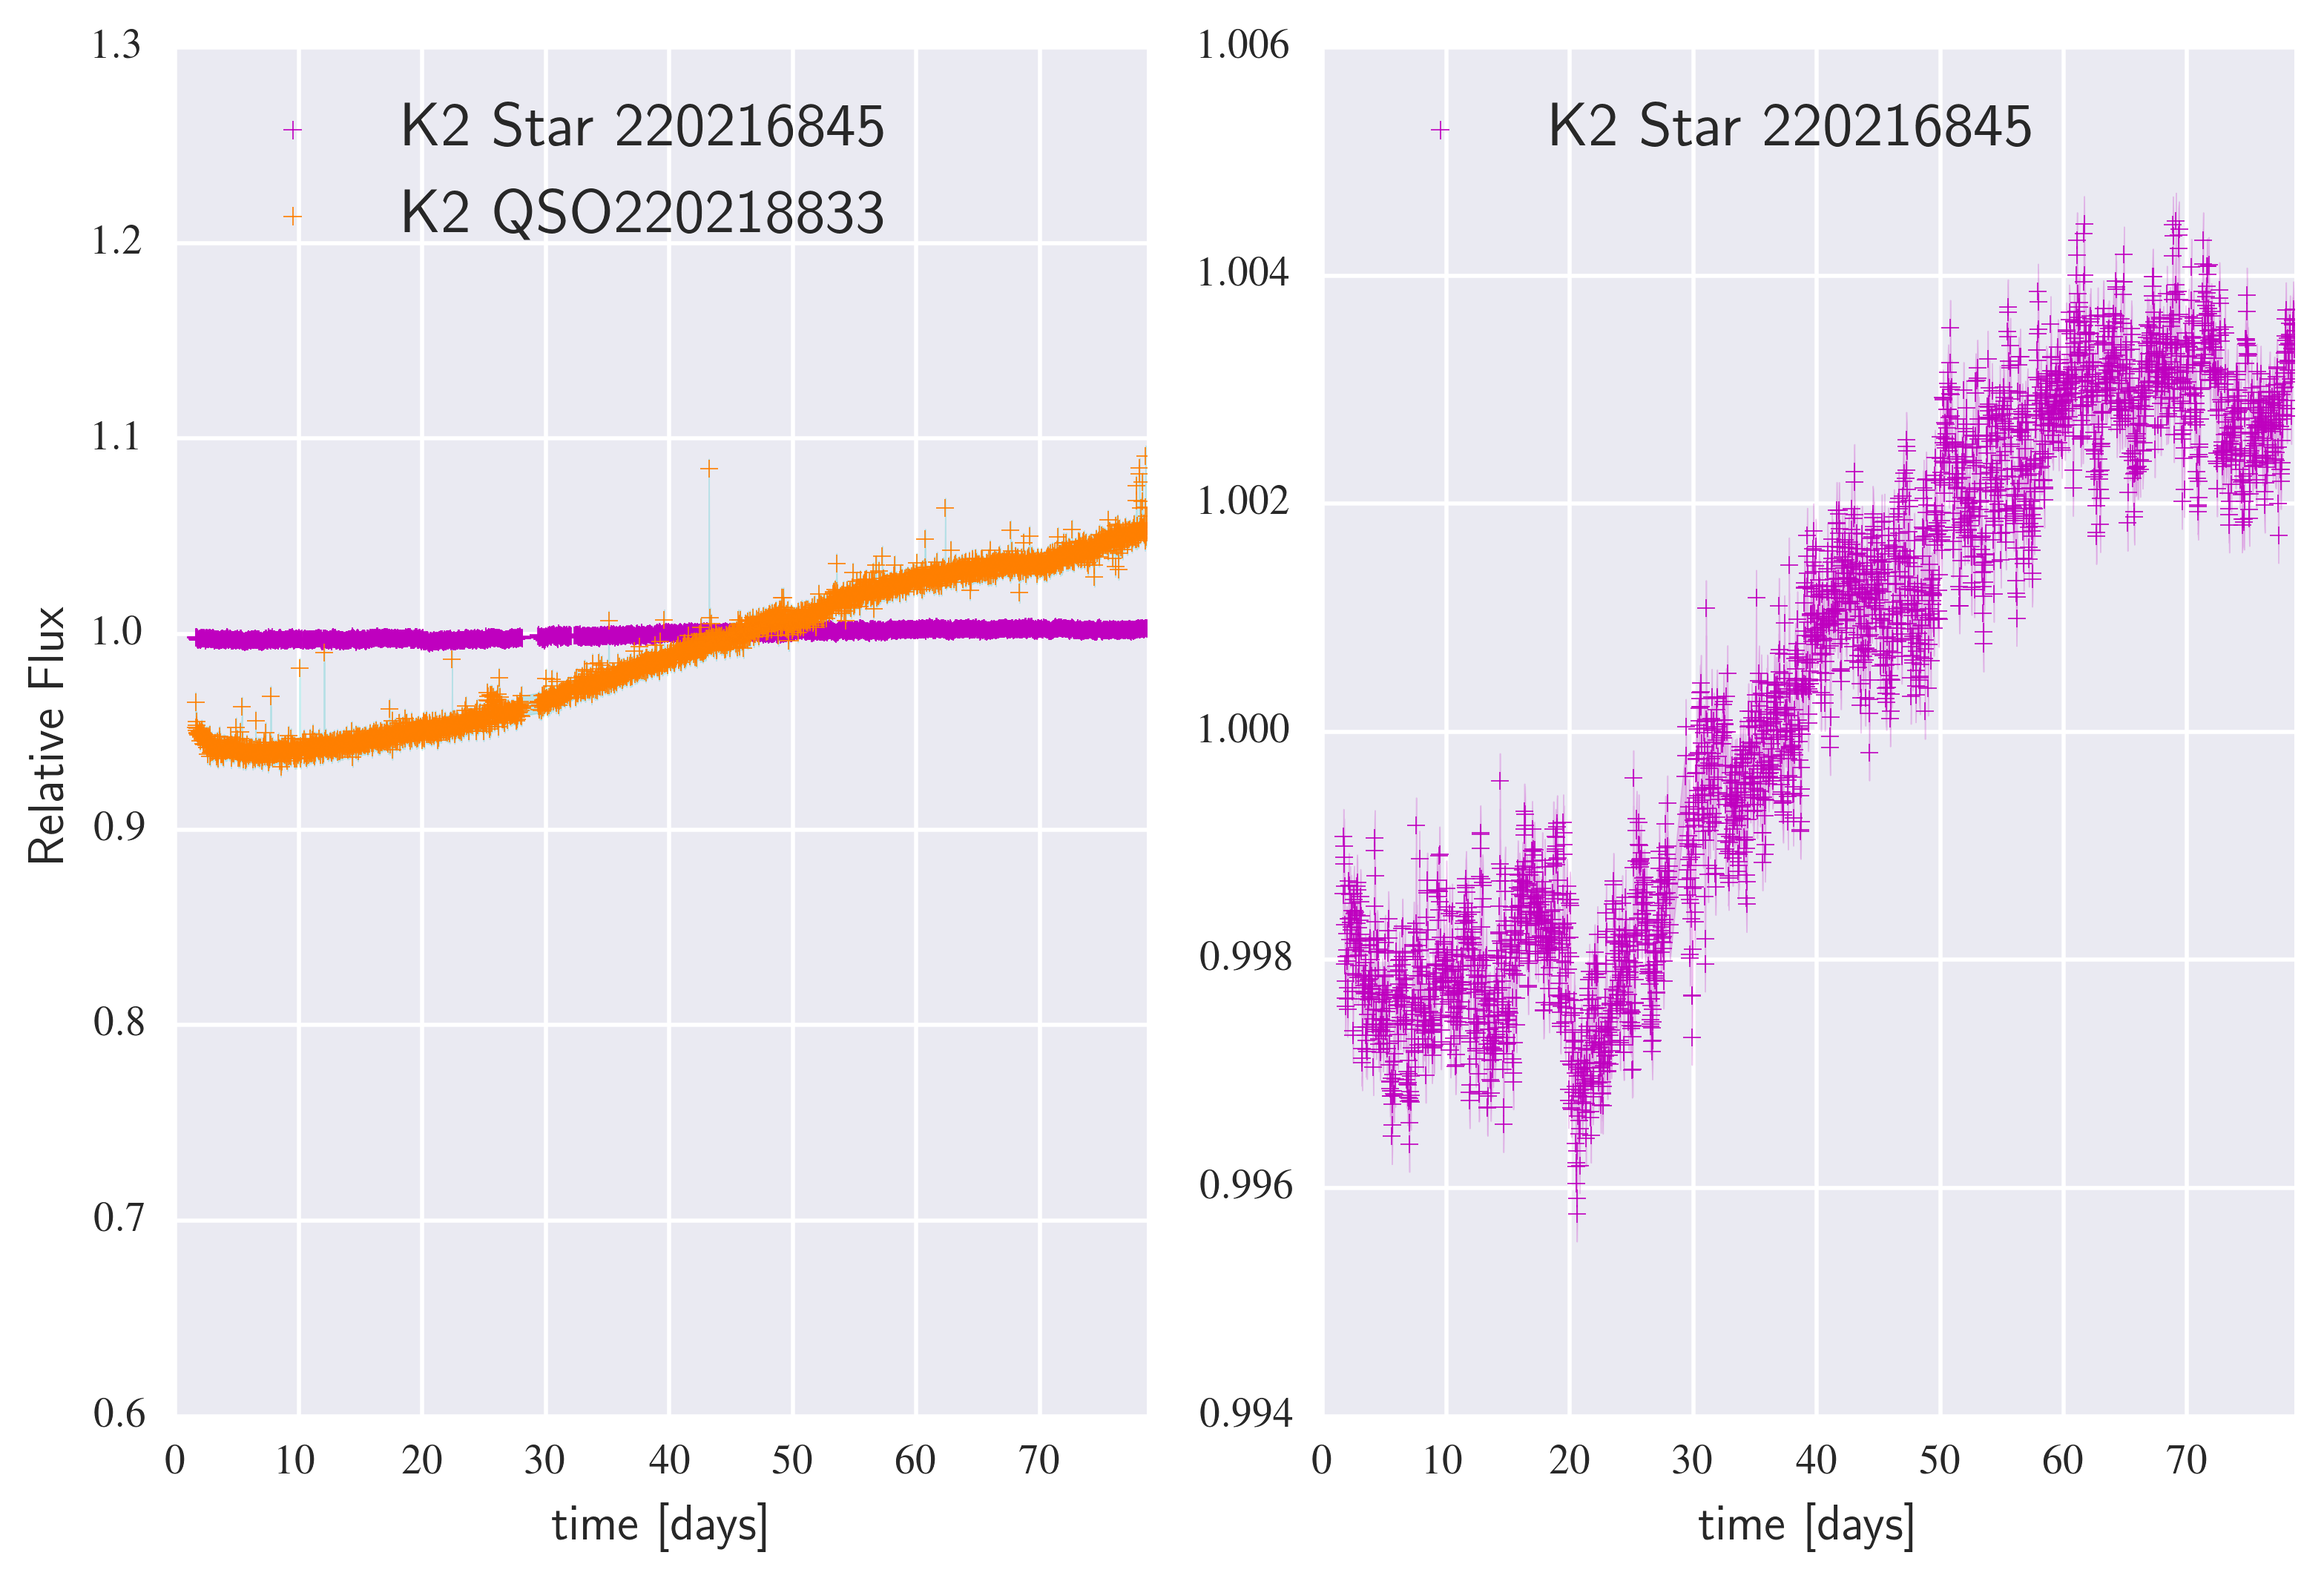
\includegraphics[width=\columnwidth]{220218833NearestNeighbor.png}
 	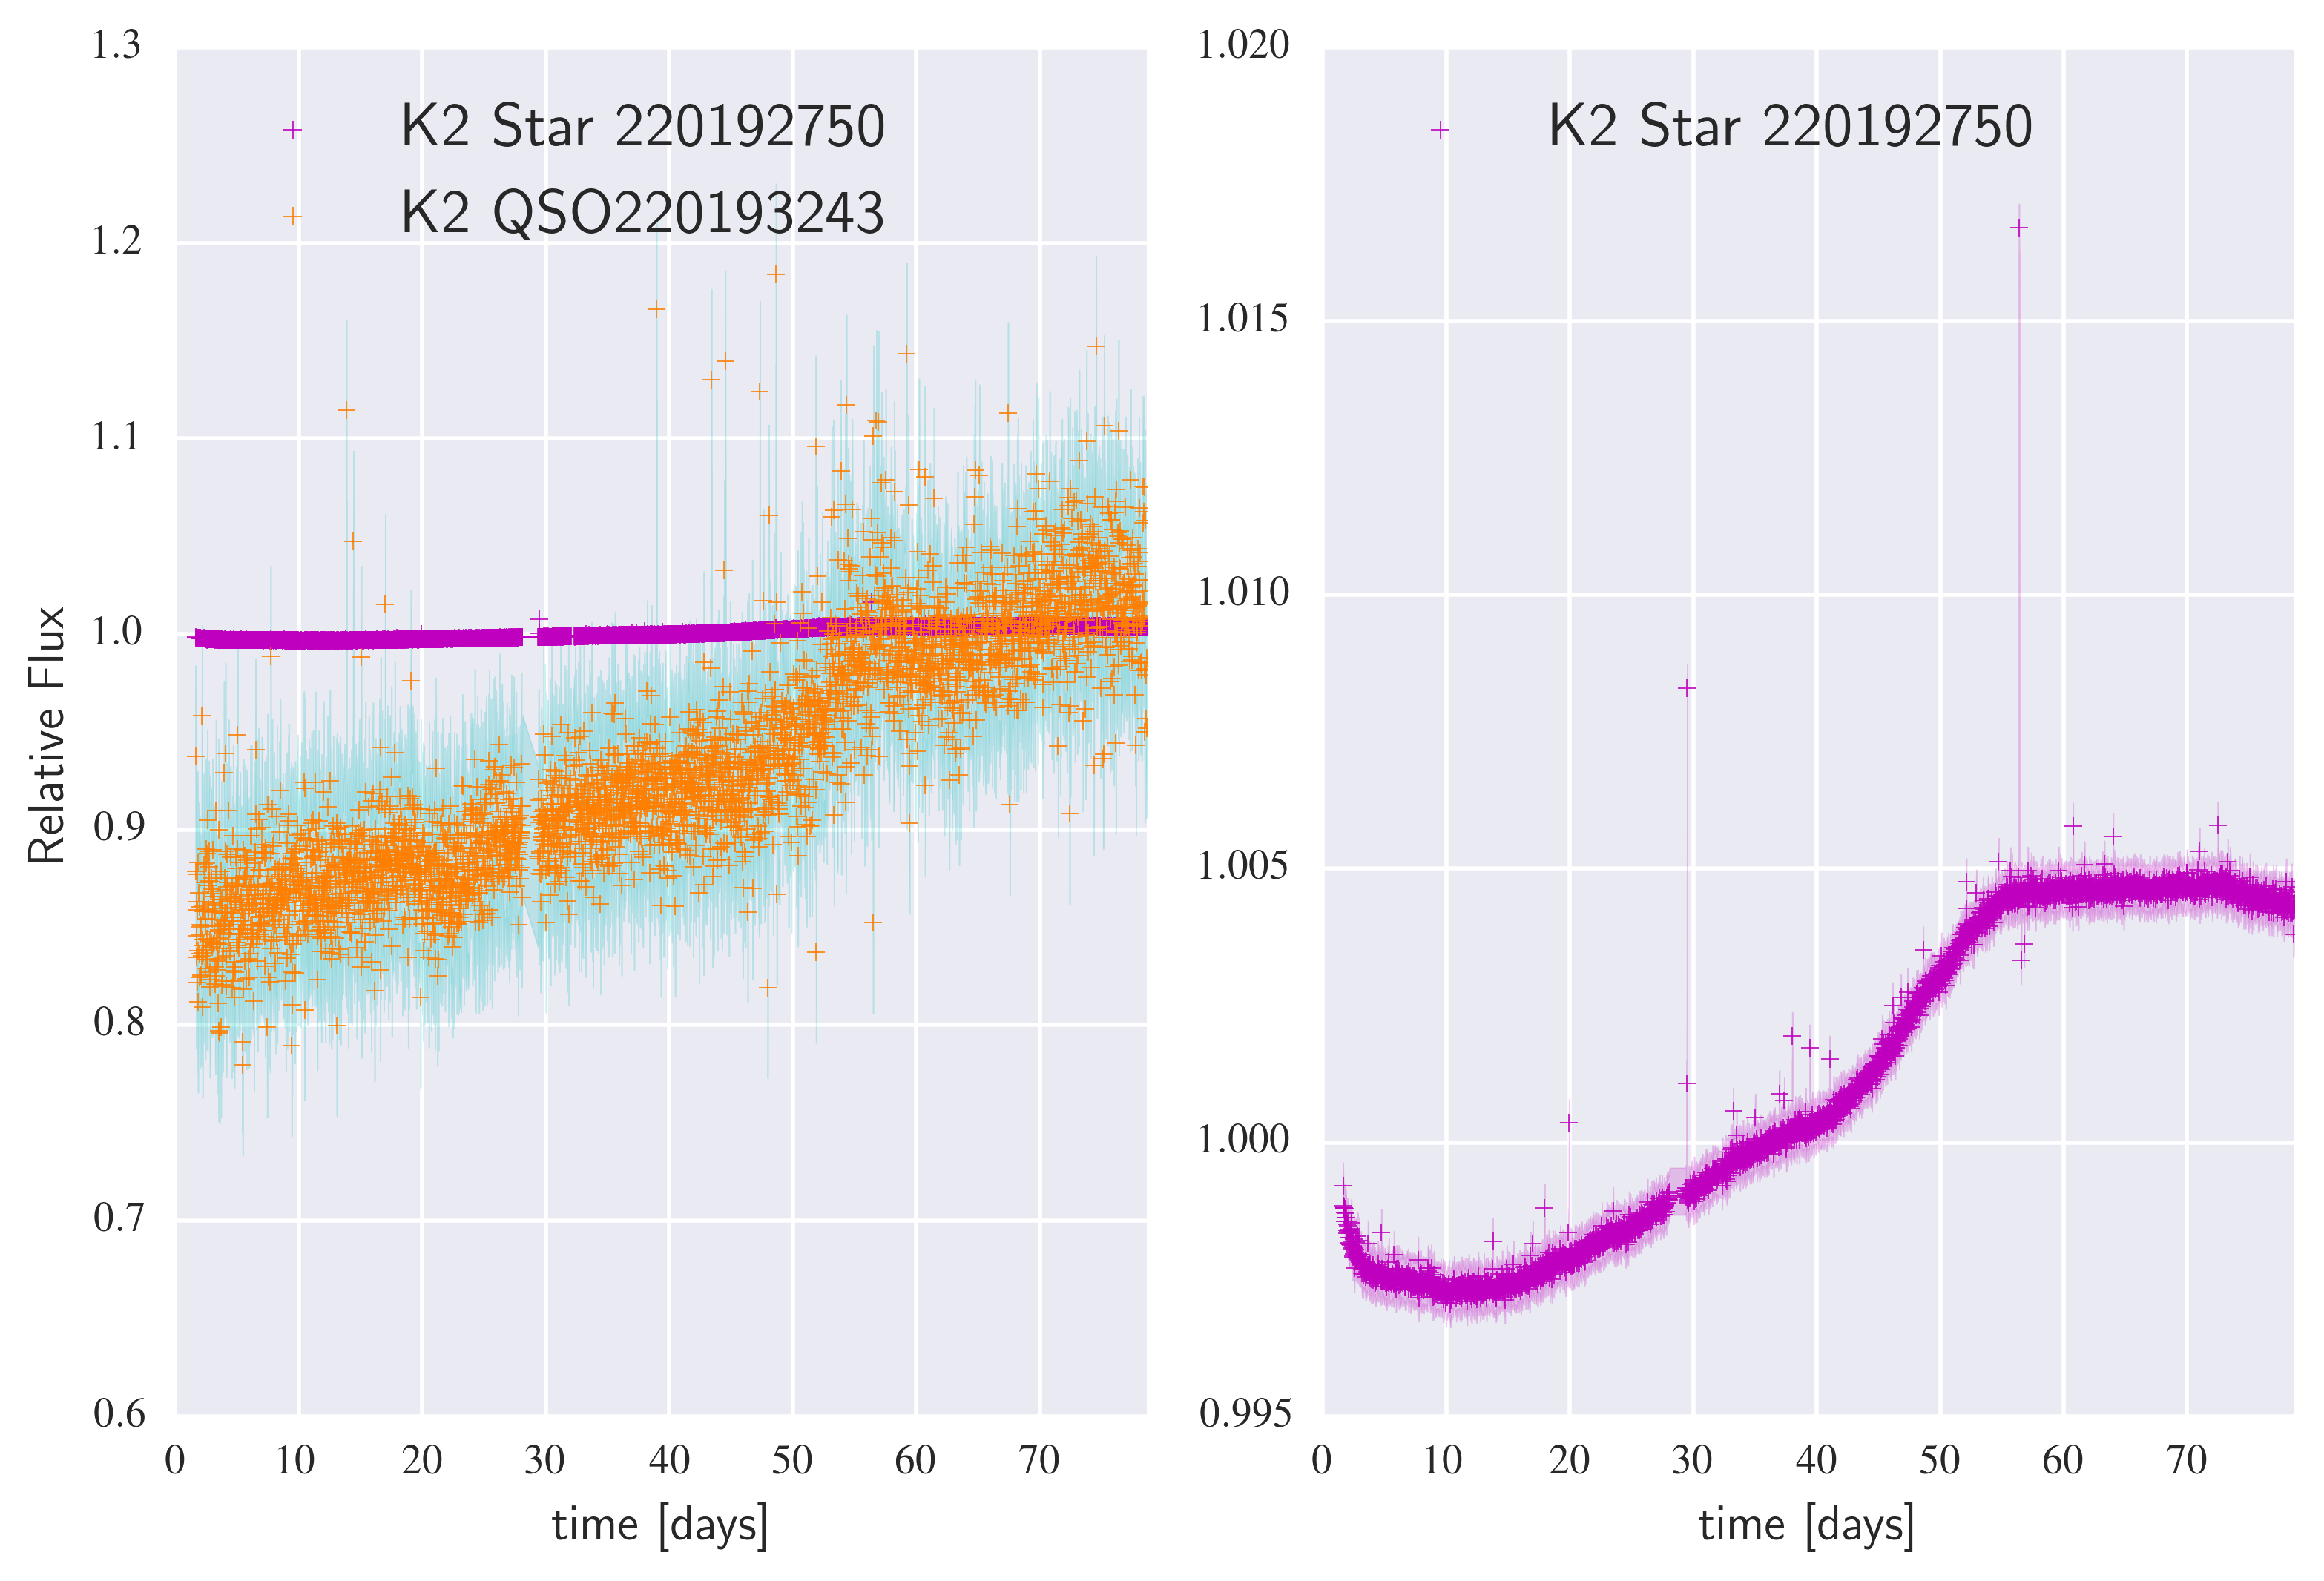
\includegraphics[width=\columnwidth]{220193243NearestNeighbor.png}
    	\label{fig:example_figure}
    \end{figure}
    
       \begin{figure}
       	% To include a figure from a file named example.*
       	% Allowable file formats are eps or ps if compiling using latex
       	% or pdf, png, jpg if compiling using pdflatex
 	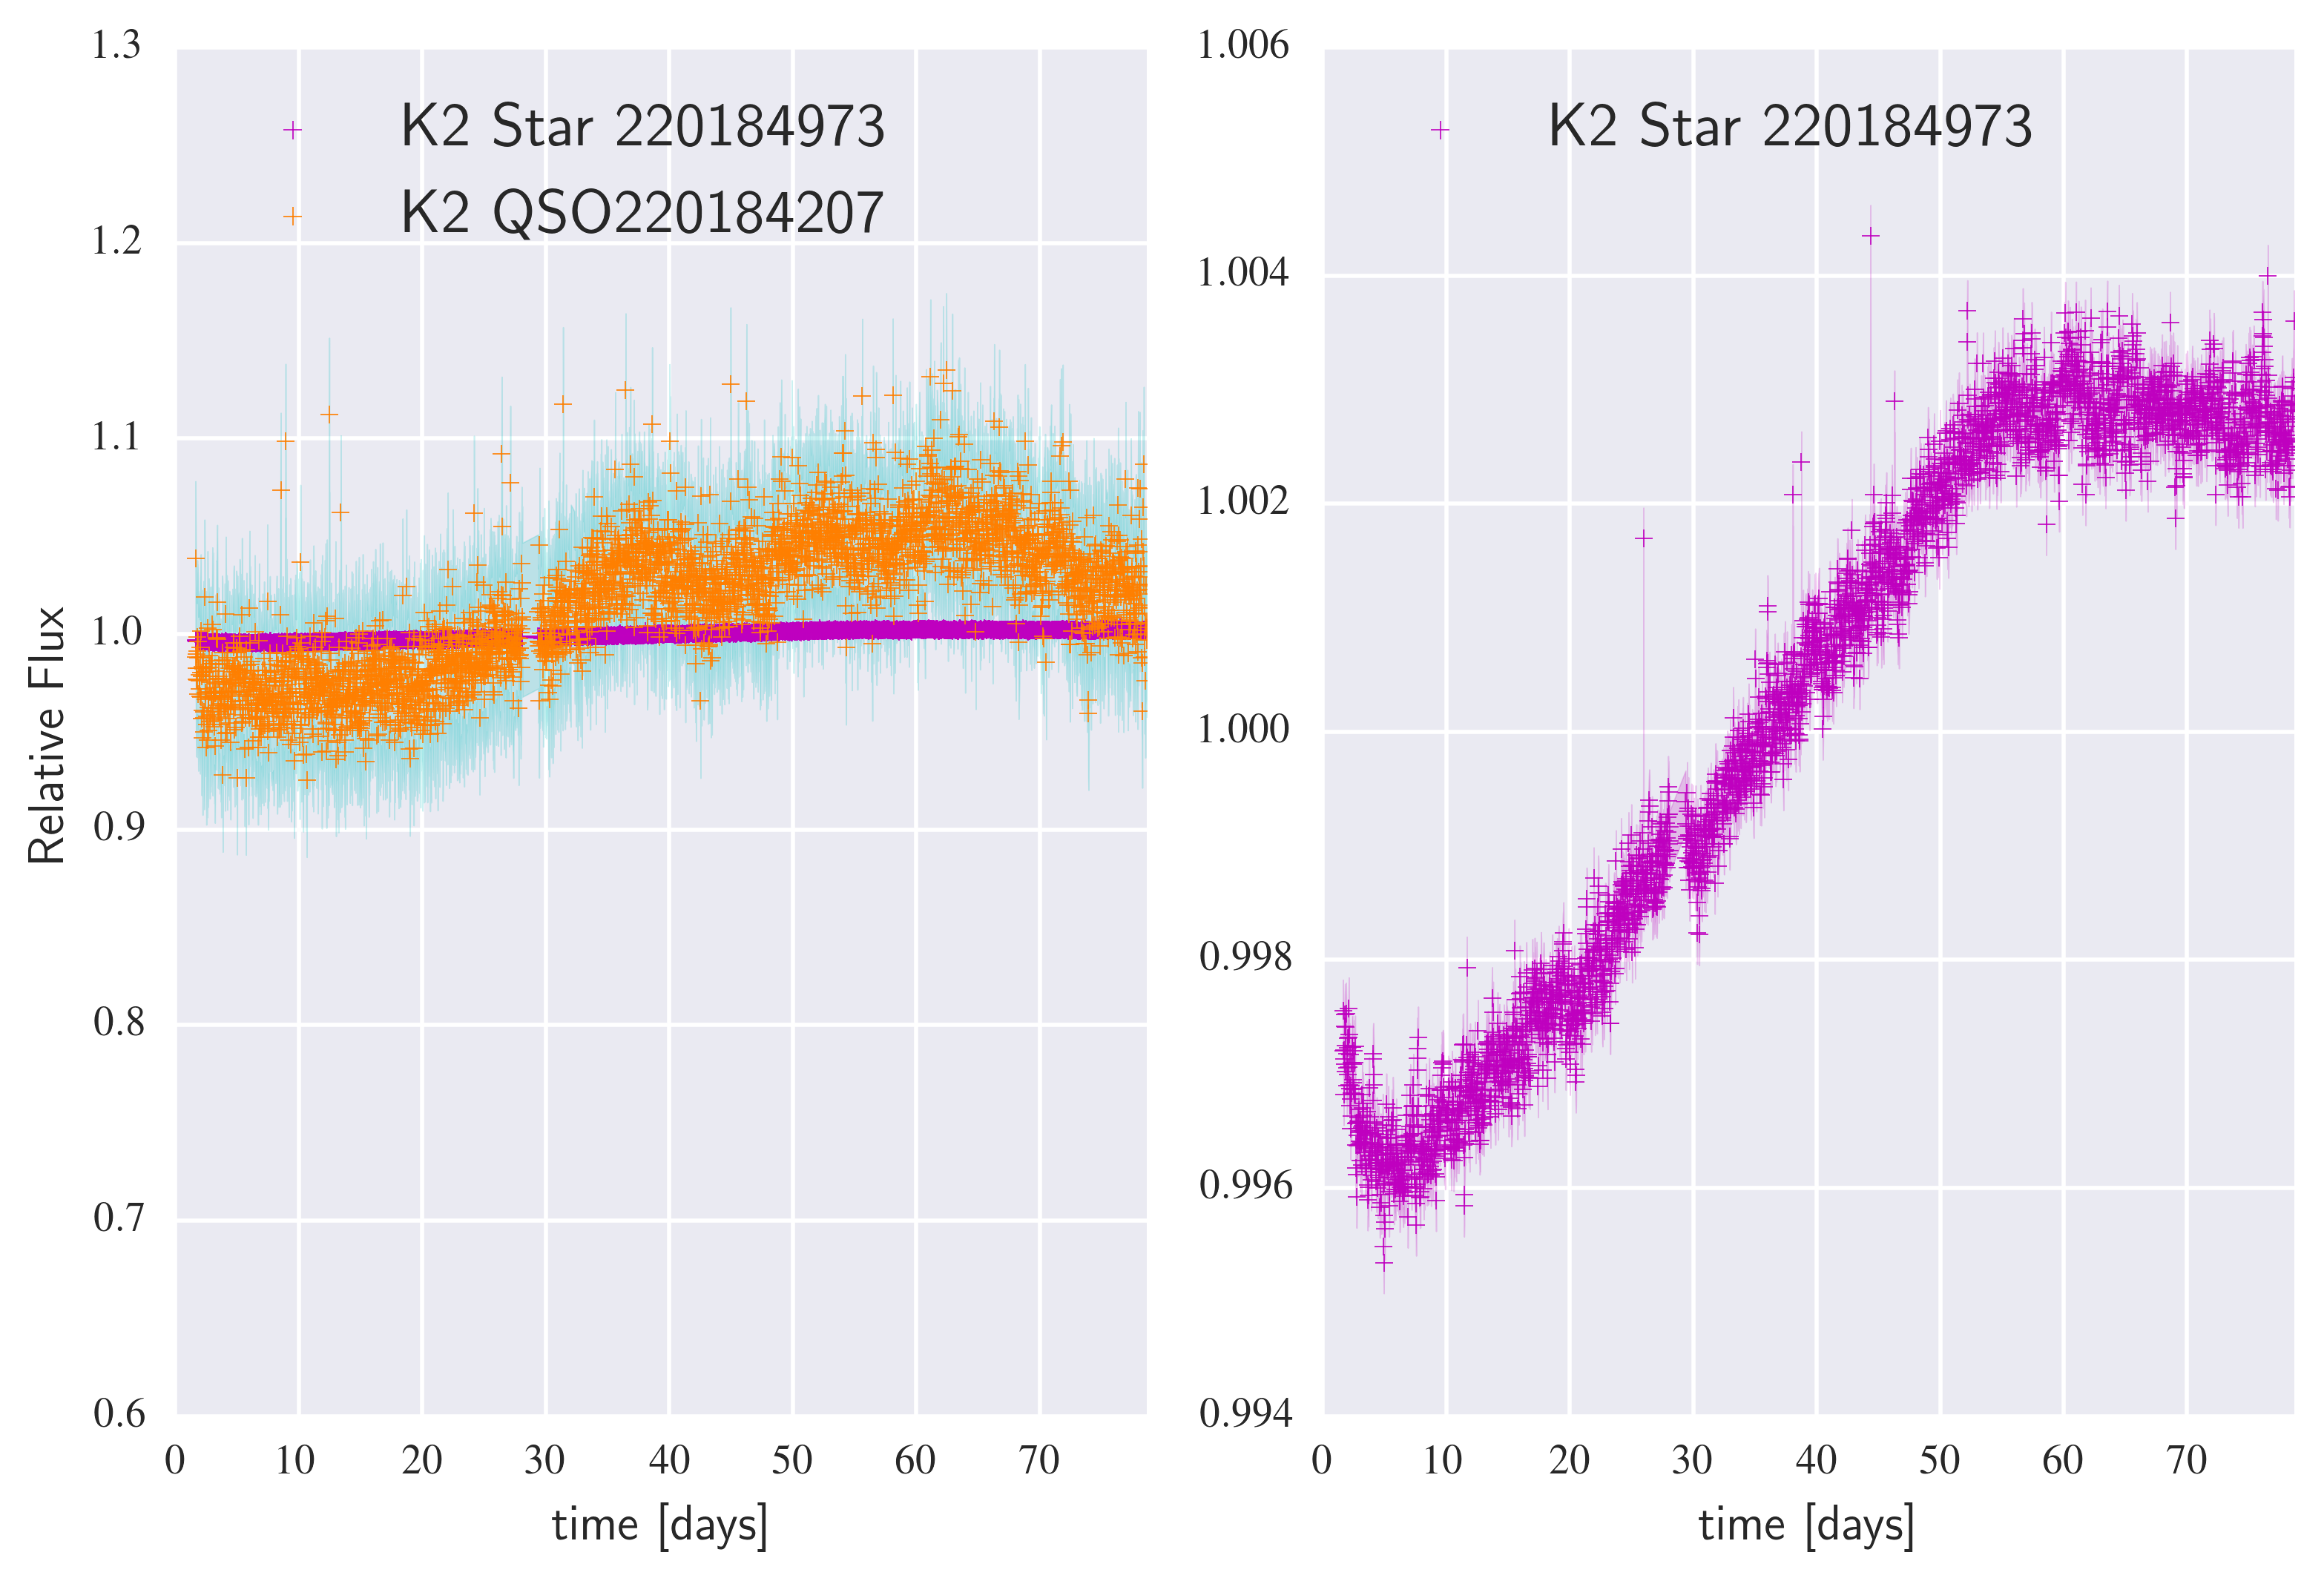
\includegraphics[width=\columnwidth]{220184207NearestNeighbor.png}
 	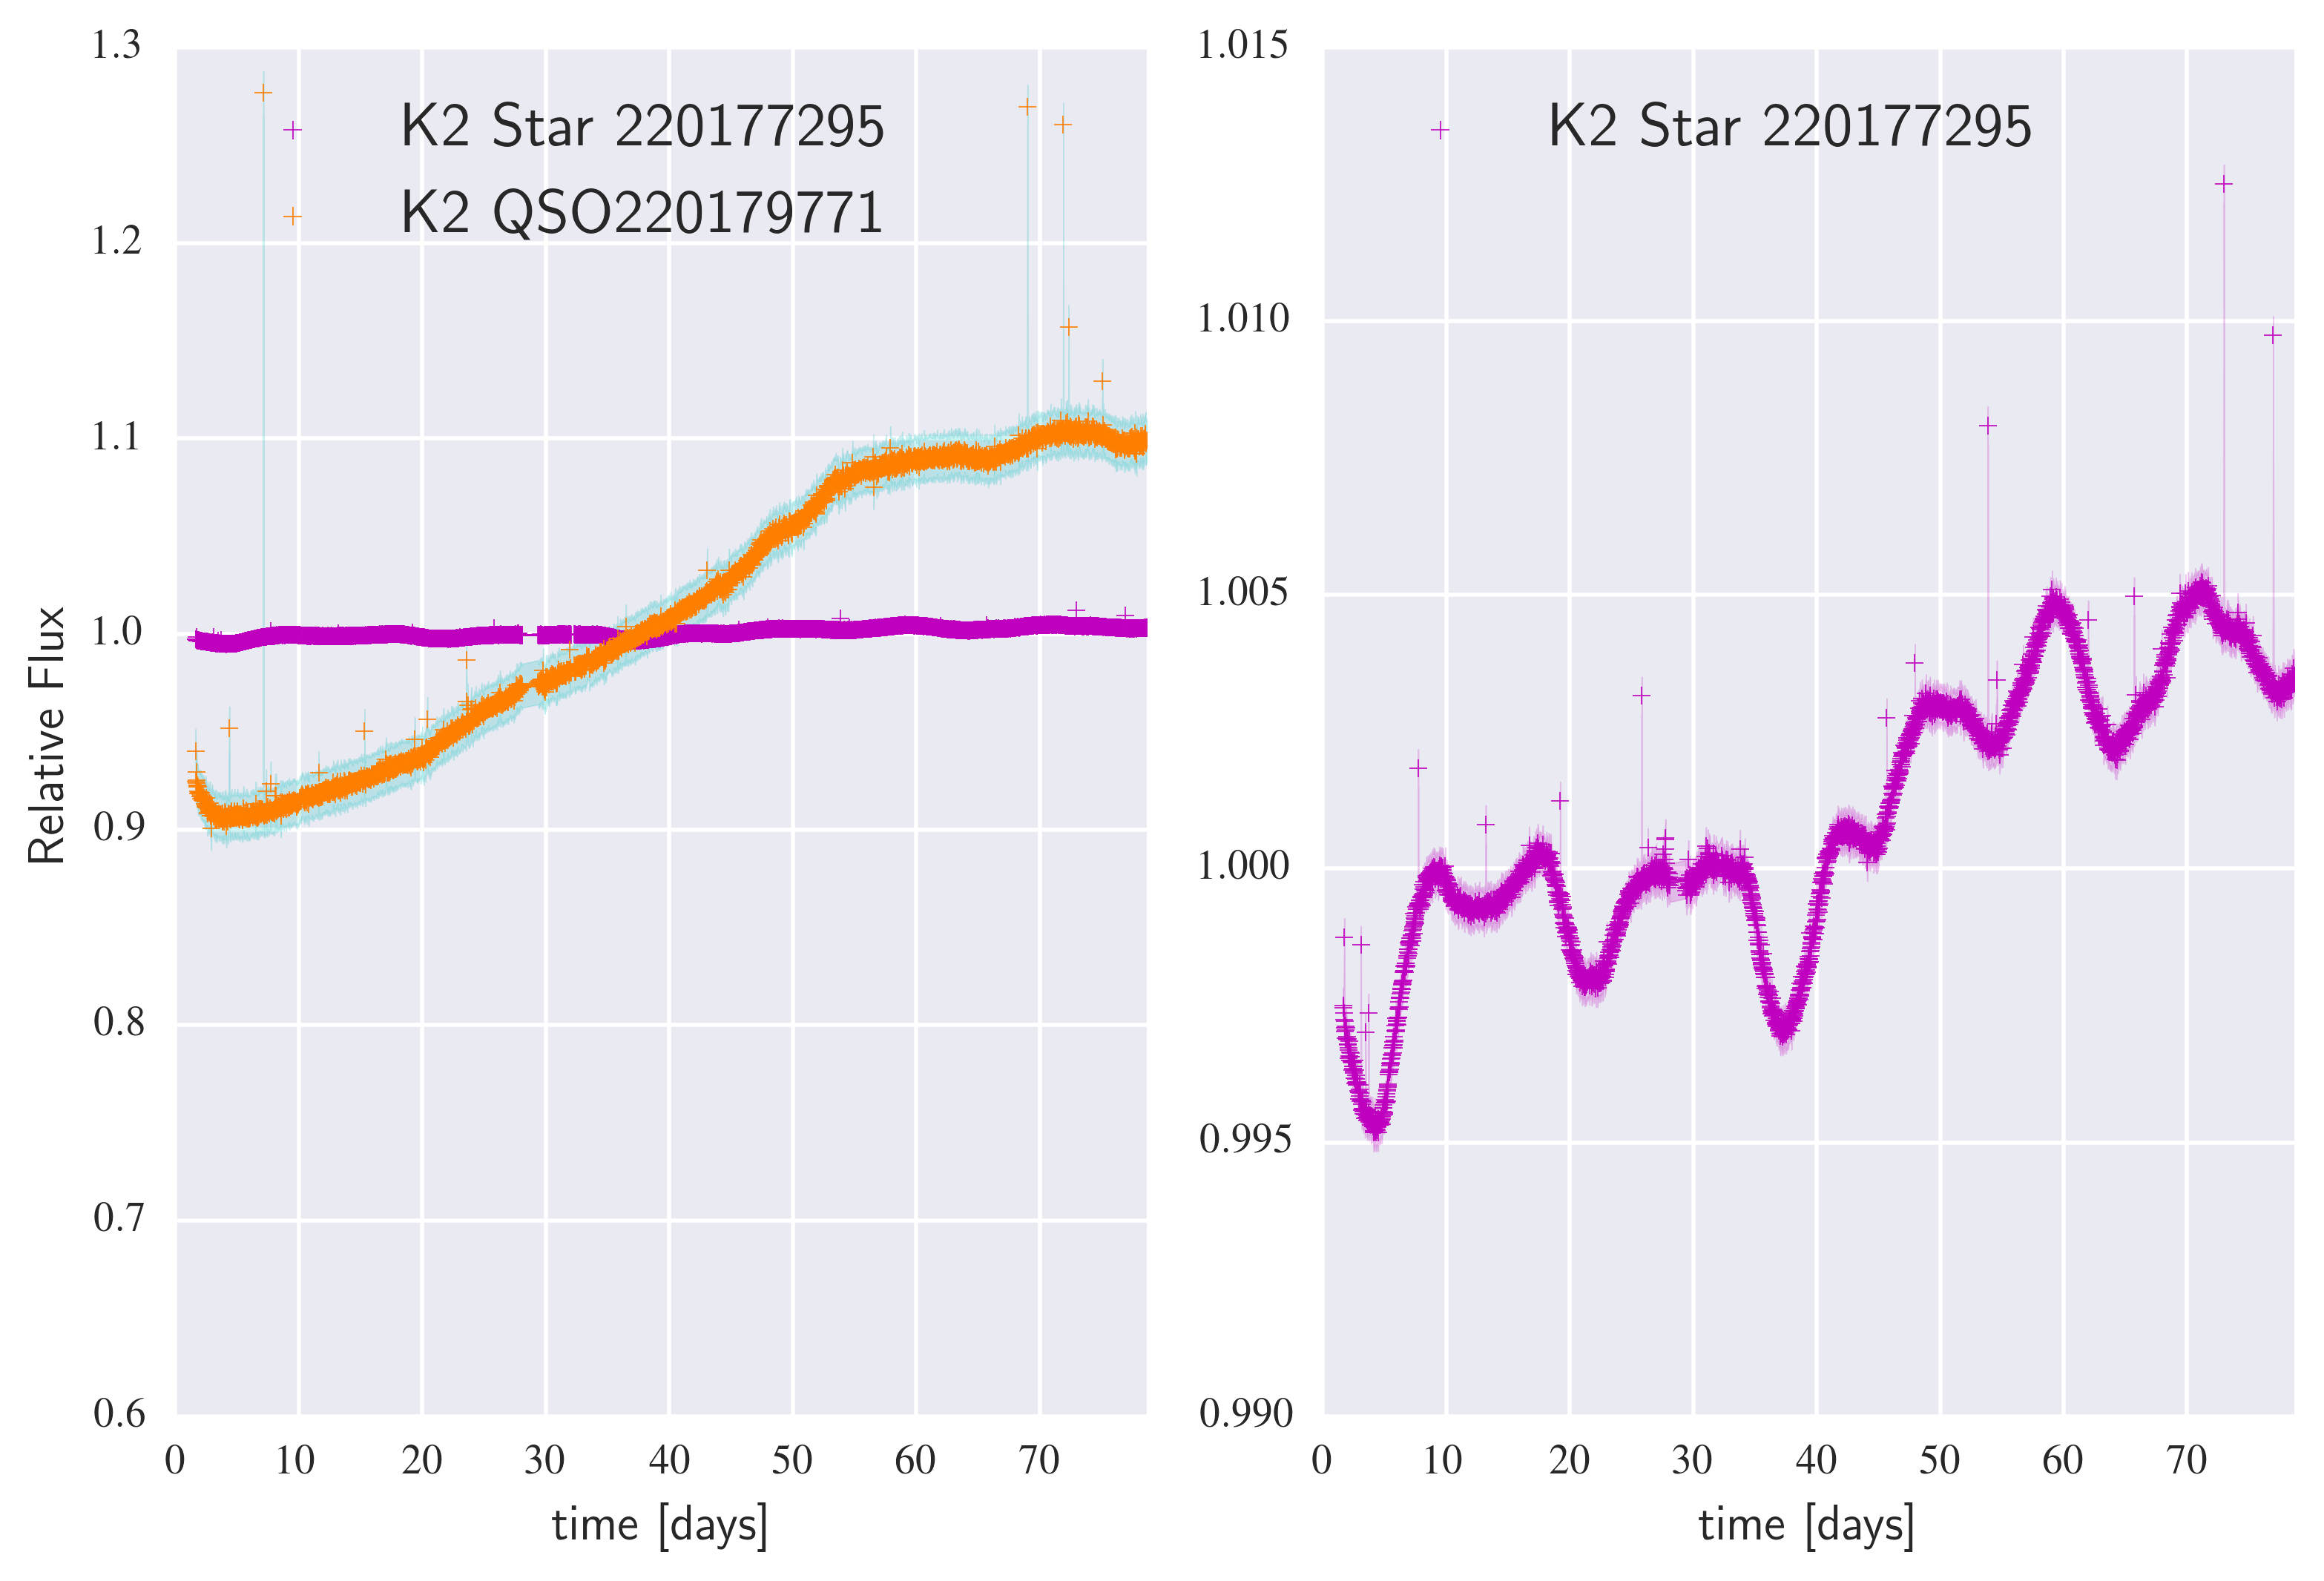
\includegraphics[width=\columnwidth]{220179771NearestNeighbor.png}
 	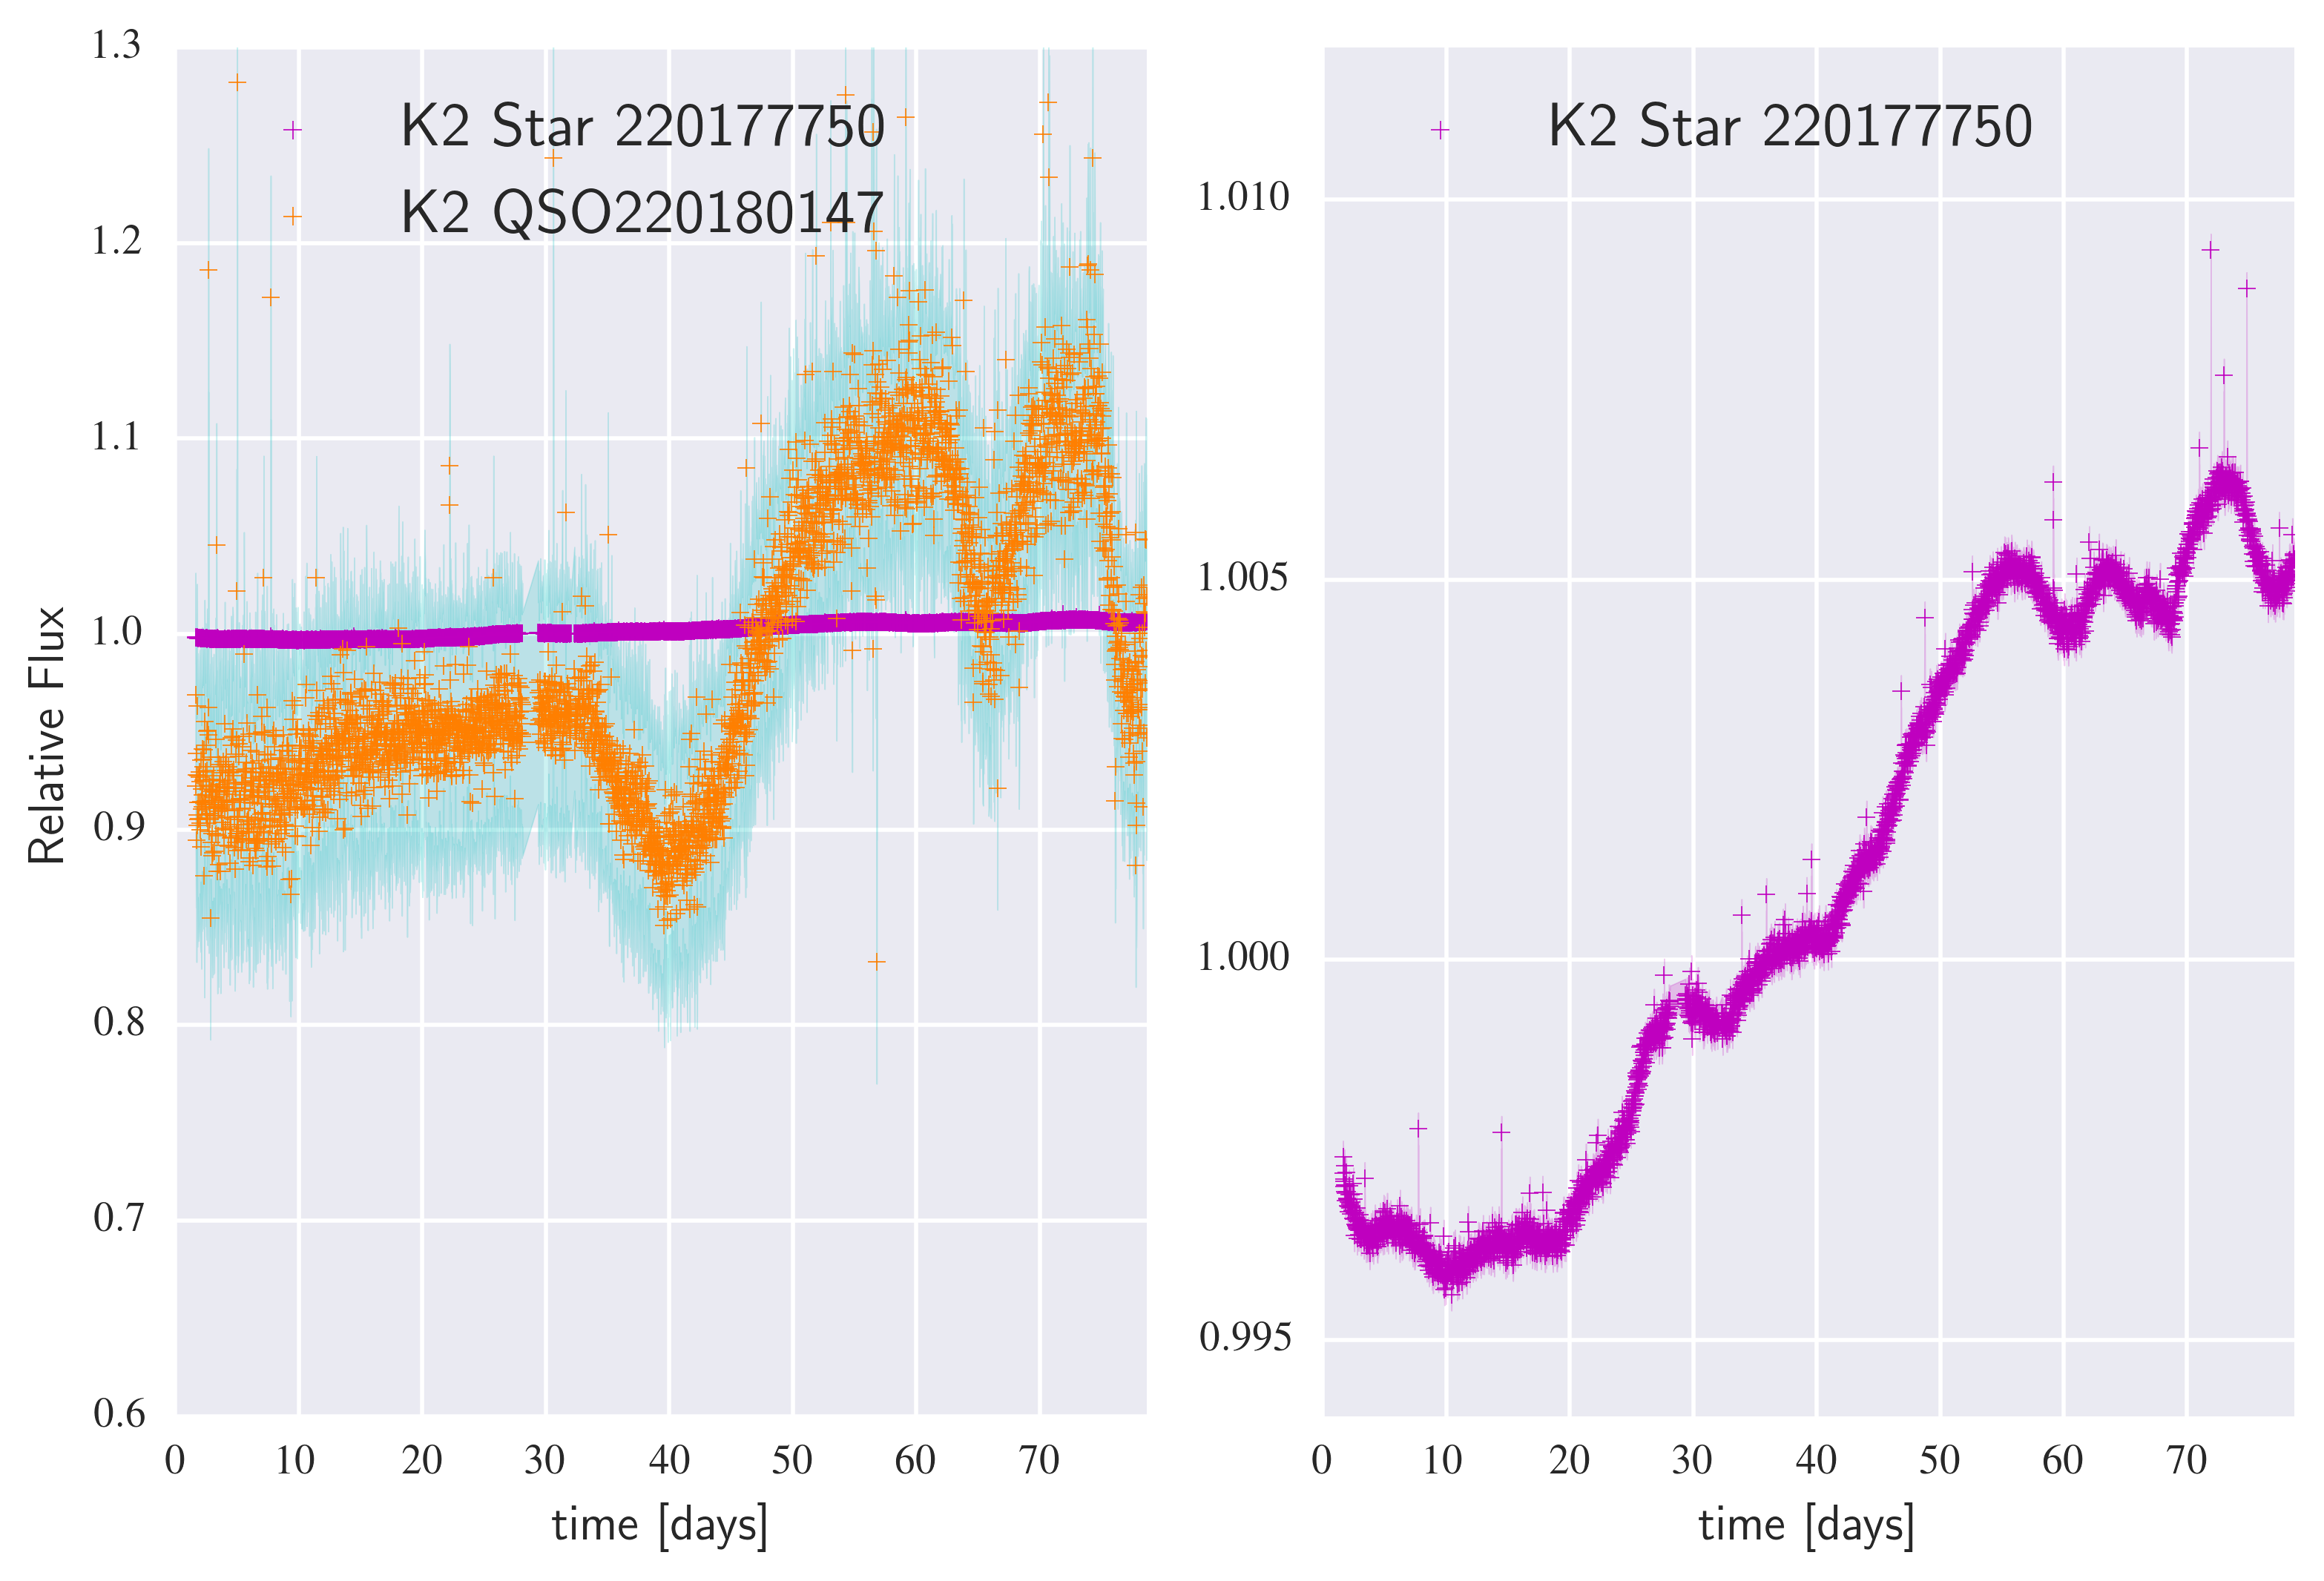
\includegraphics[width=\columnwidth]{220180147NearestNeighbor.png}
       	\caption{}
       	\label{fig:example_figure}
       \end{figure}

          
          
          
                    \begin{figure}
                    	% To include a figure from a file named example.*
                    	% Allowable file formats are eps or ps if compiling using latex
                    	% or pdf, png, jpg if compiling using pdflatex
 	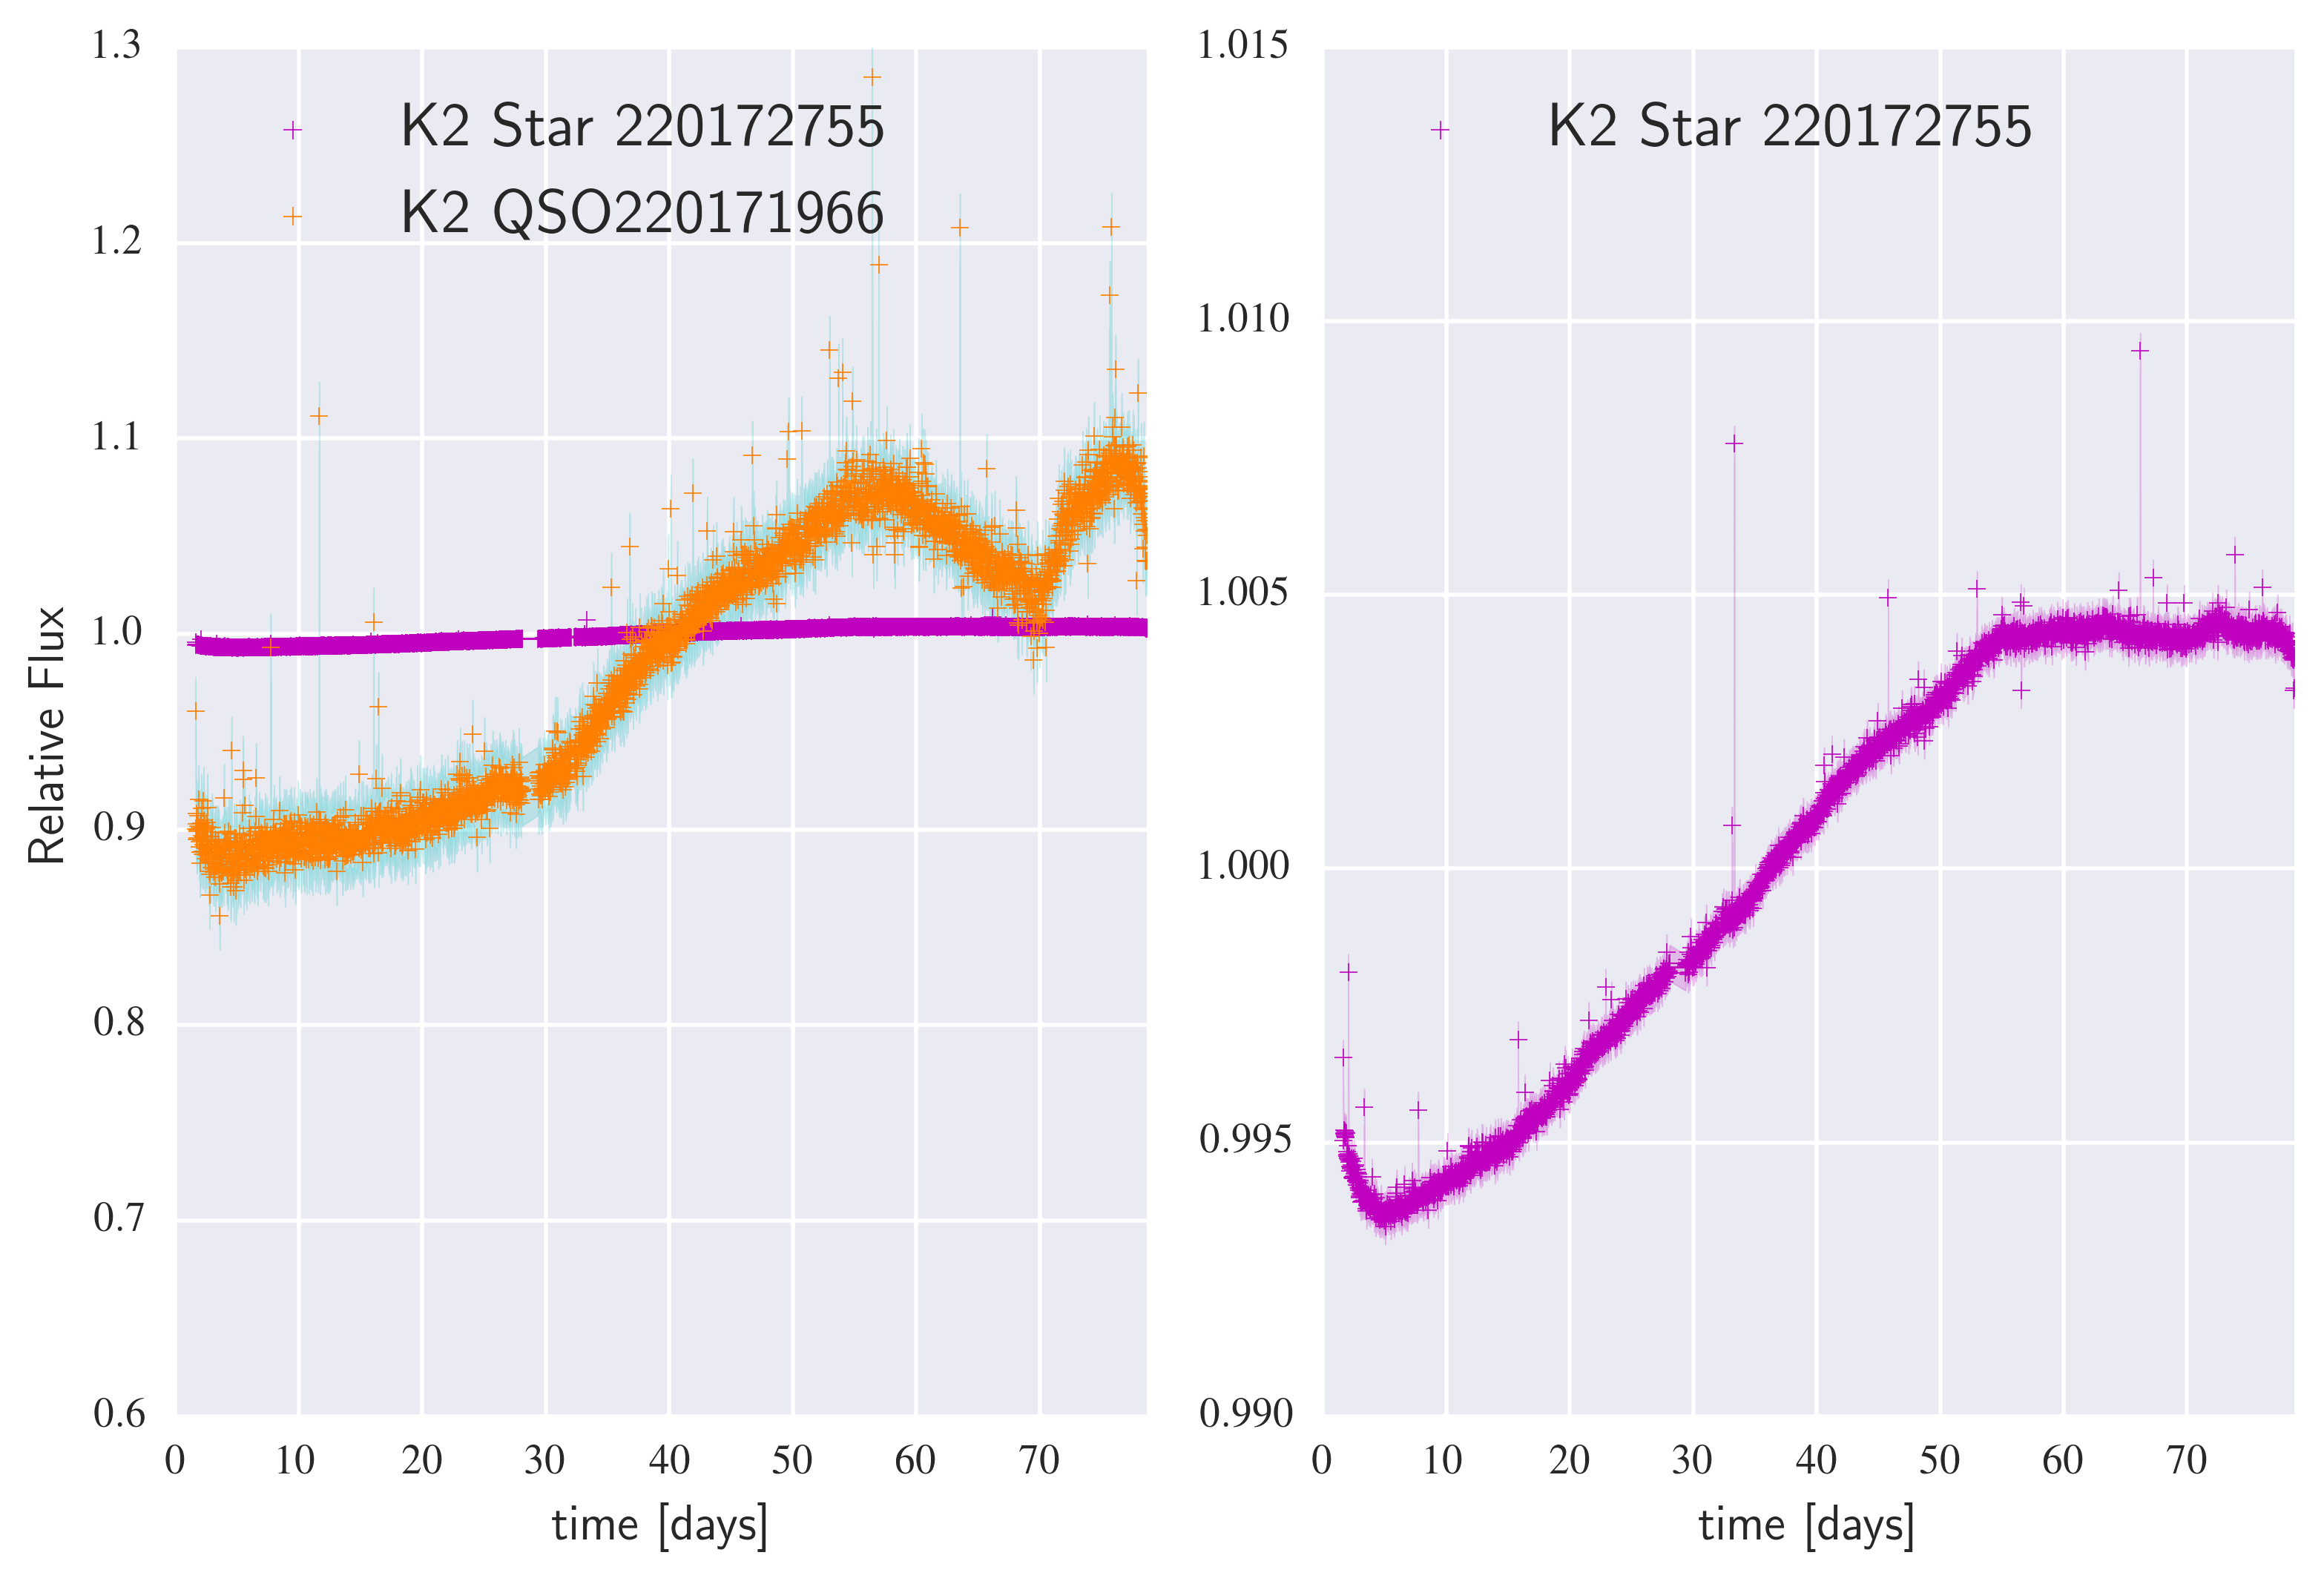
\includegraphics[width=\columnwidth]{220171966NearestNeighbor.png}
 	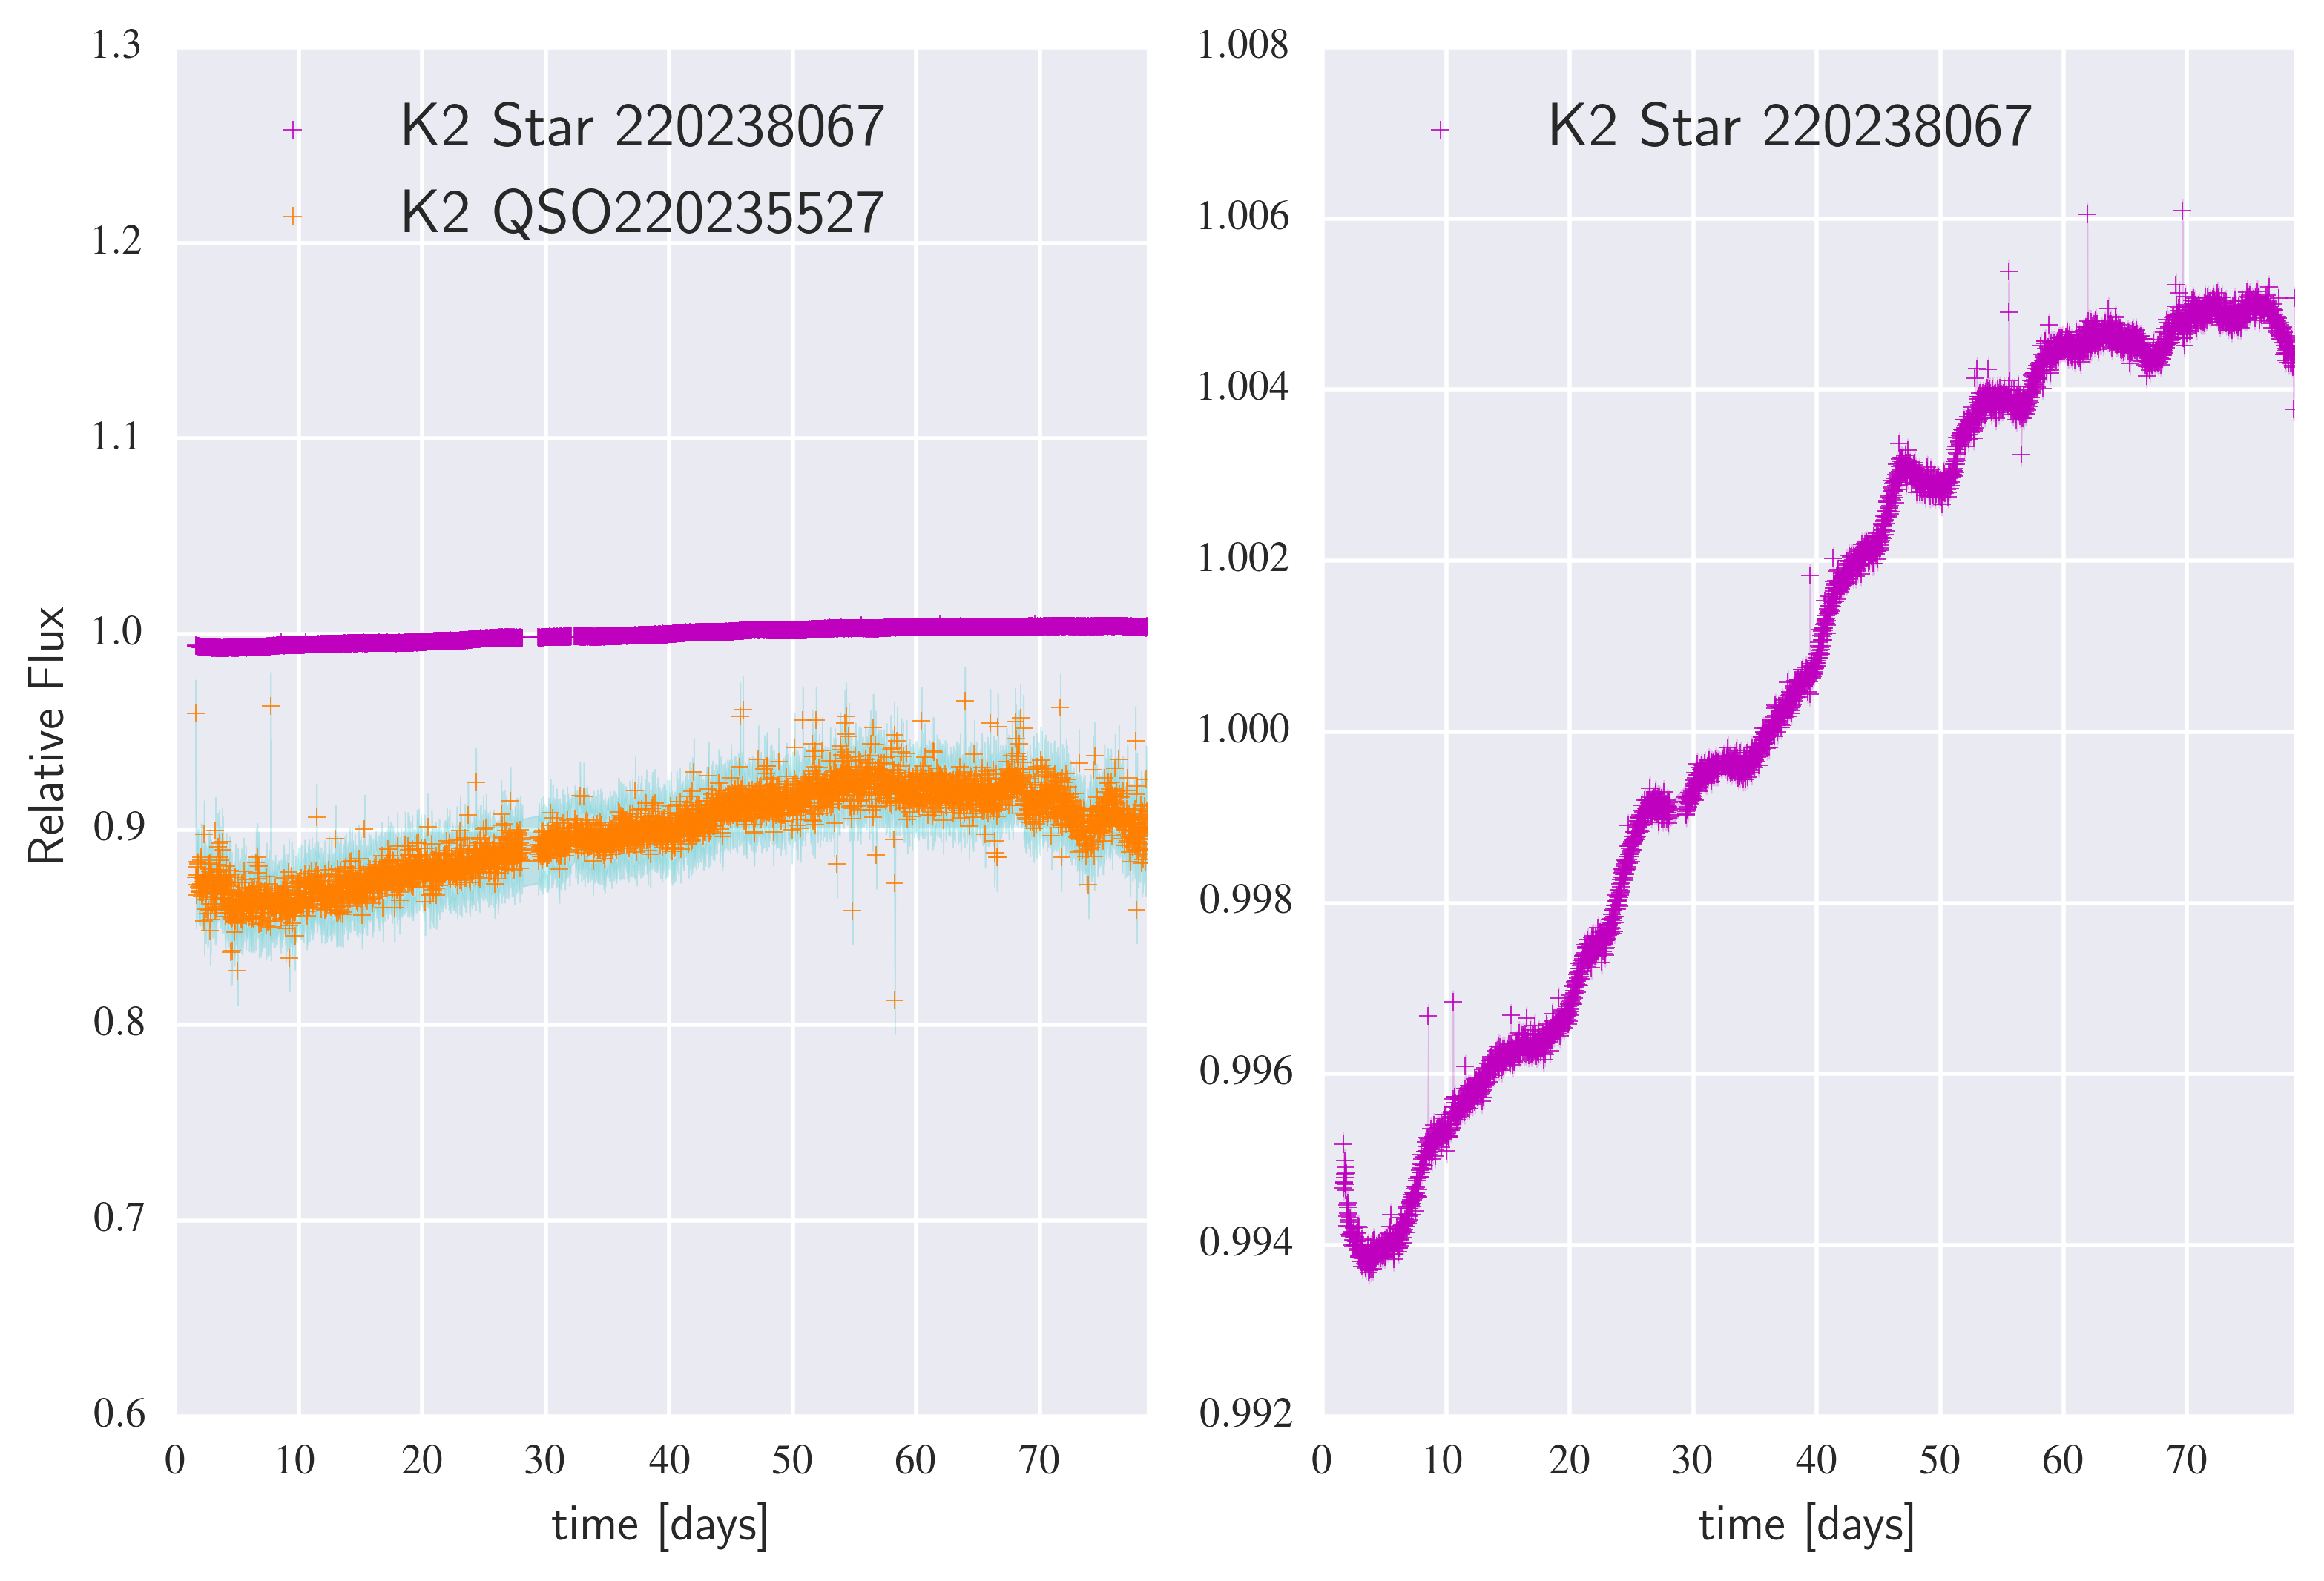
\includegraphics[width=\columnwidth]{220235527NearestNeighbor.png}
 	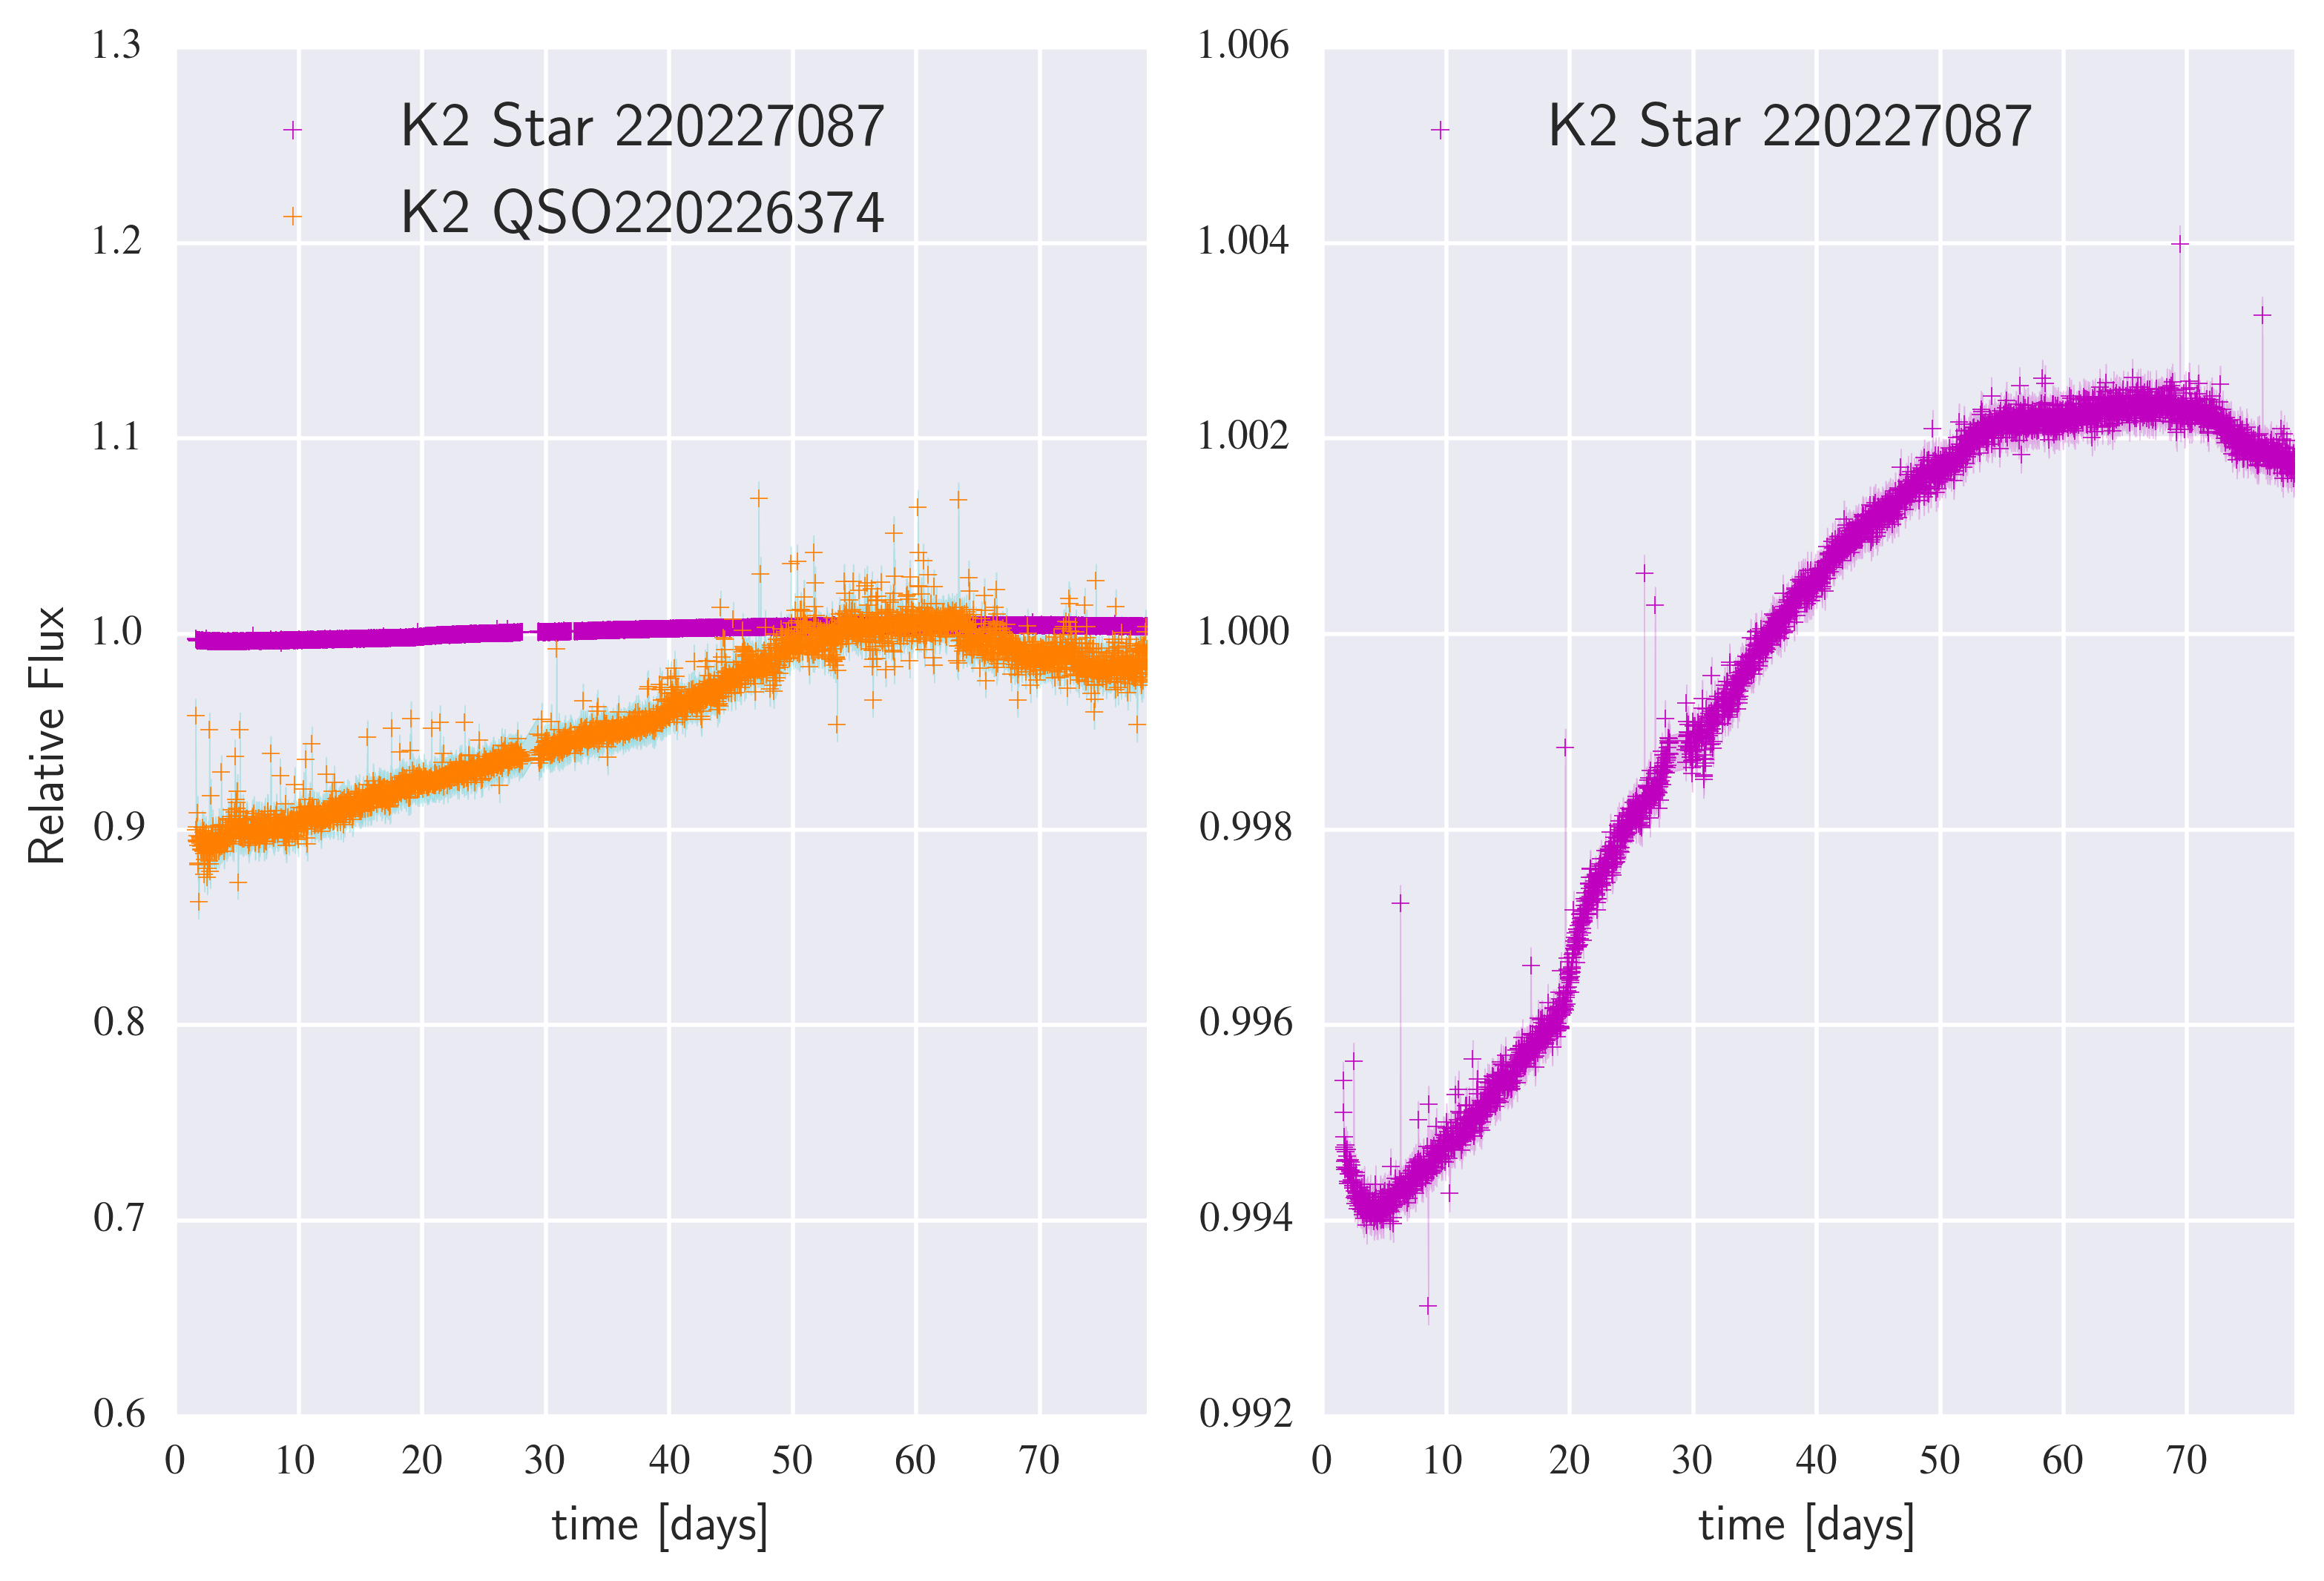
\includegraphics[width=\columnwidth]{220226374NearestNeighbor.png}
                    	\caption{}
                    	\label{fig:example_figure}
                    \end{figure}
                    
          \begin{figure}
          	% To include a figure from a file named example.*
          	% Allowable file formats are eps or ps if compiling using latex
          	% or pdf, png, jpg if compiling using pdflatex
  	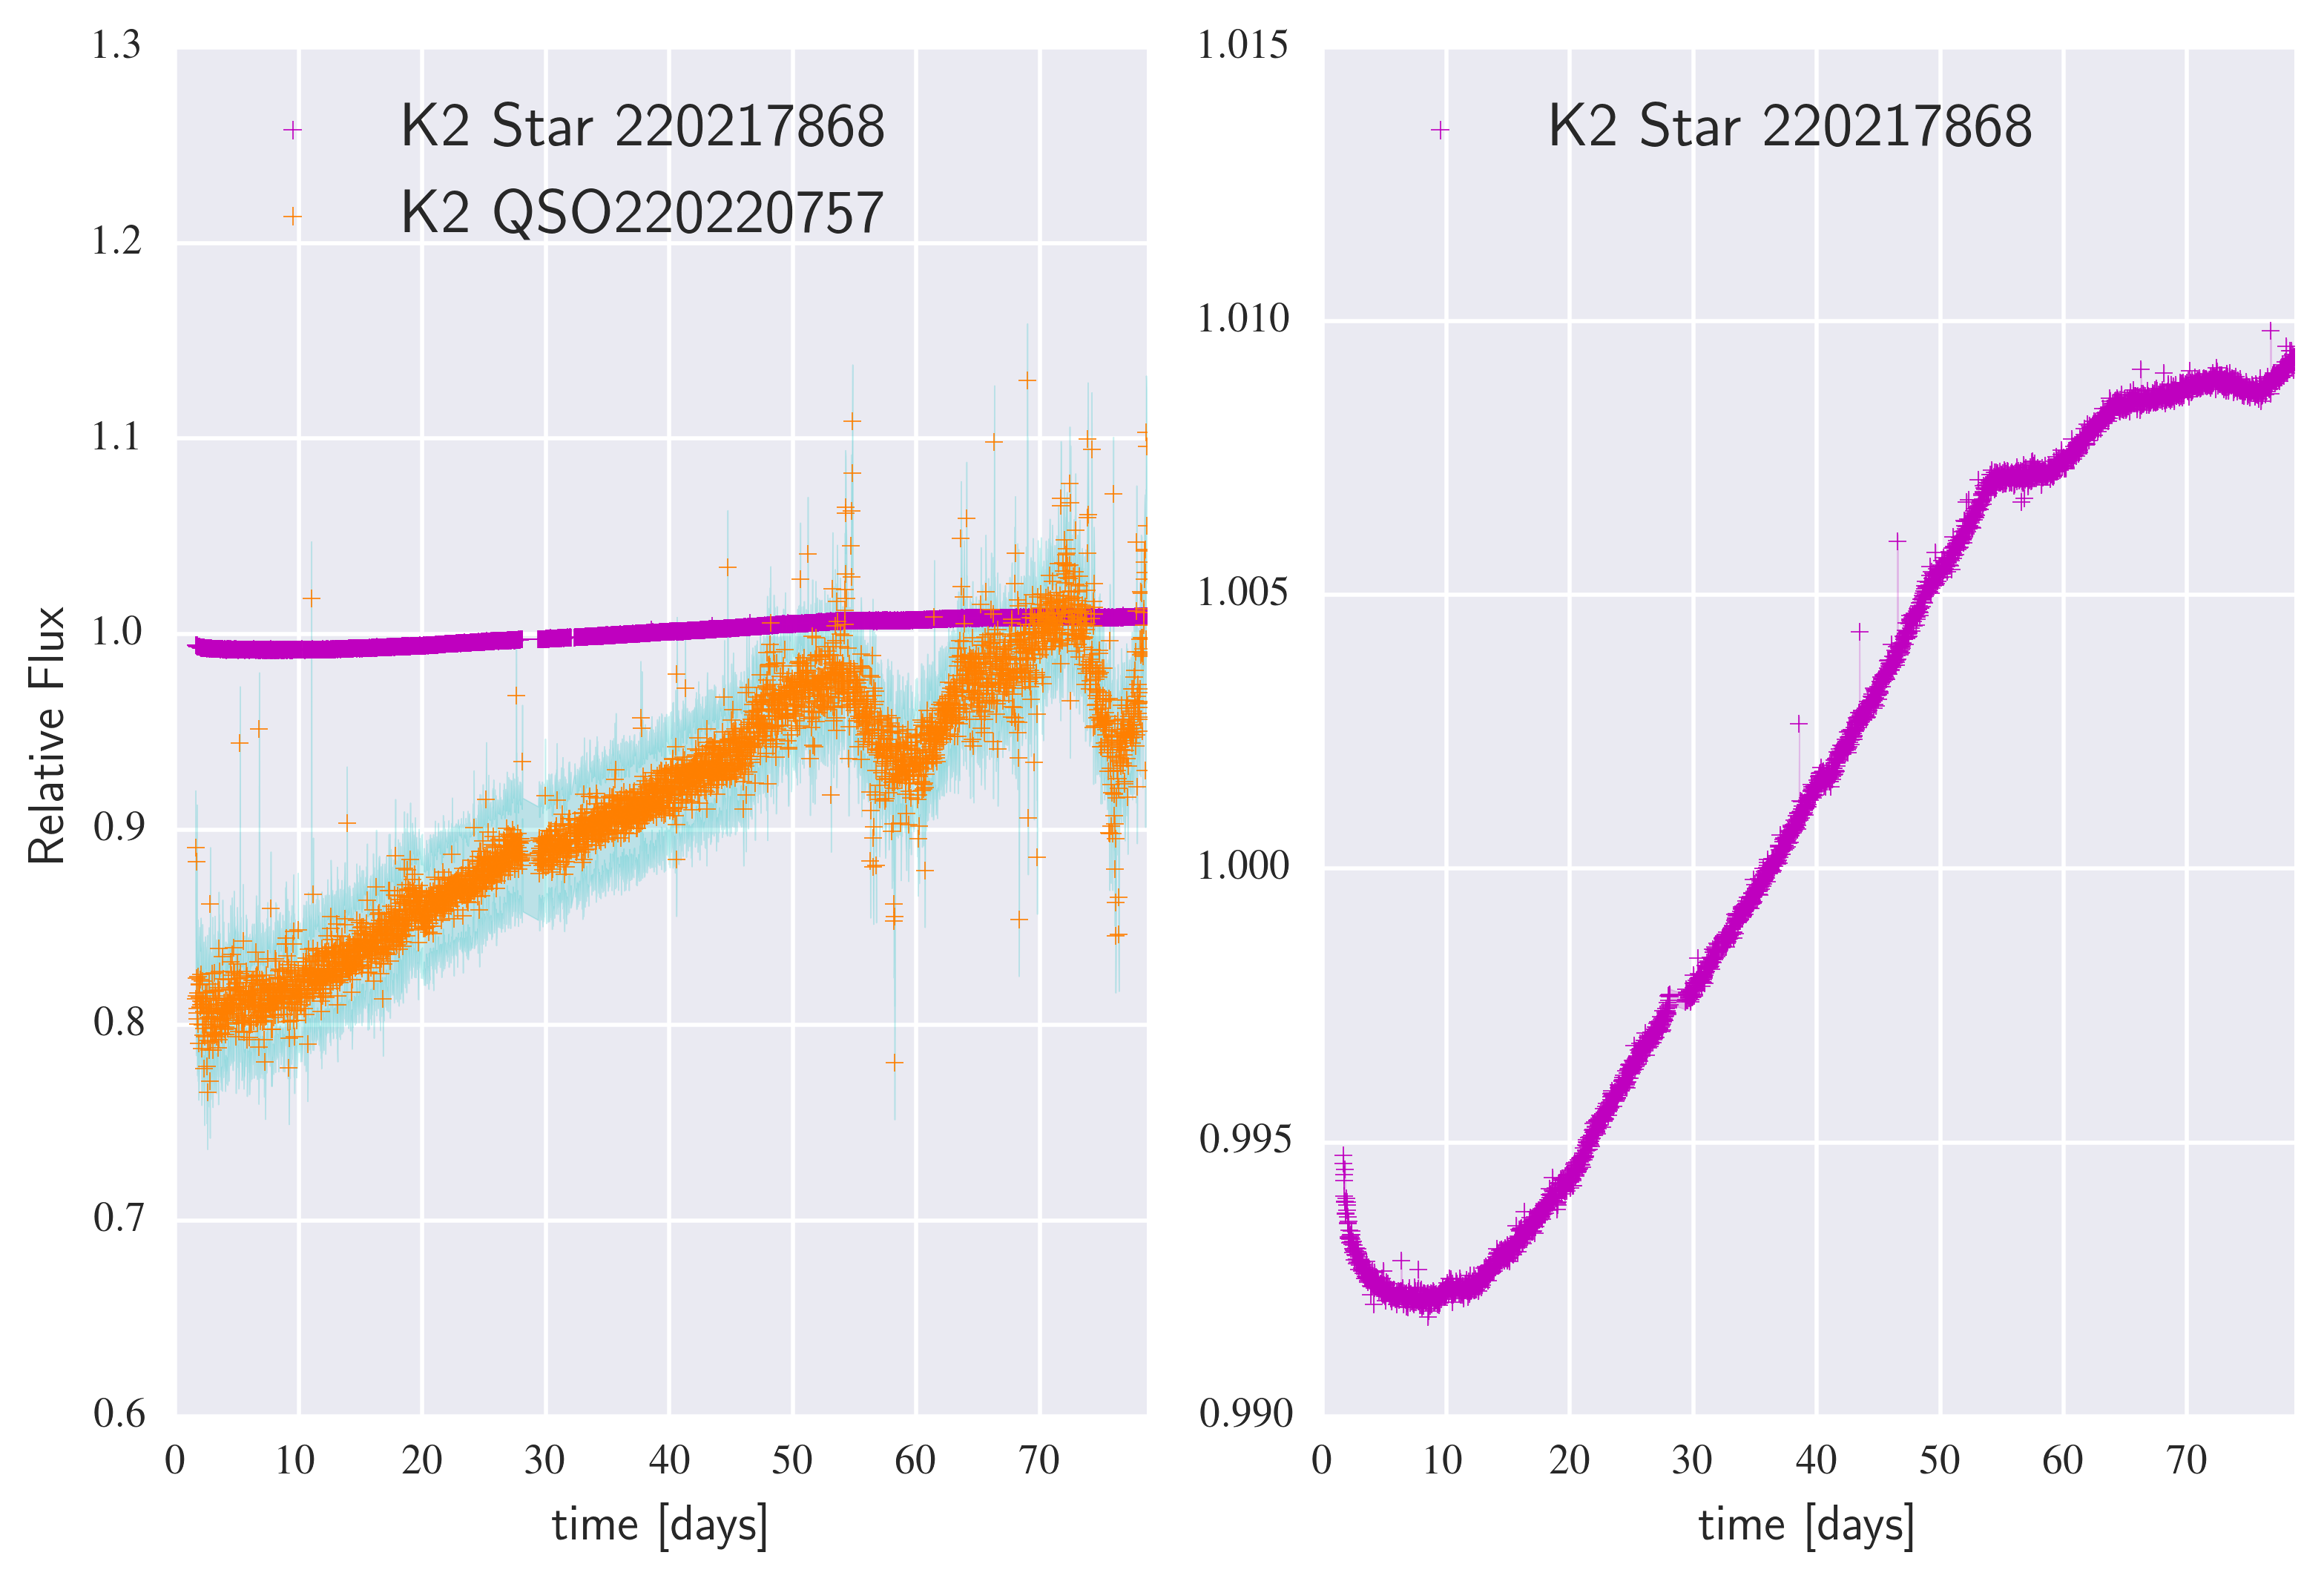
\includegraphics[width=\columnwidth]{220220757NearestNeighbor.png}
  	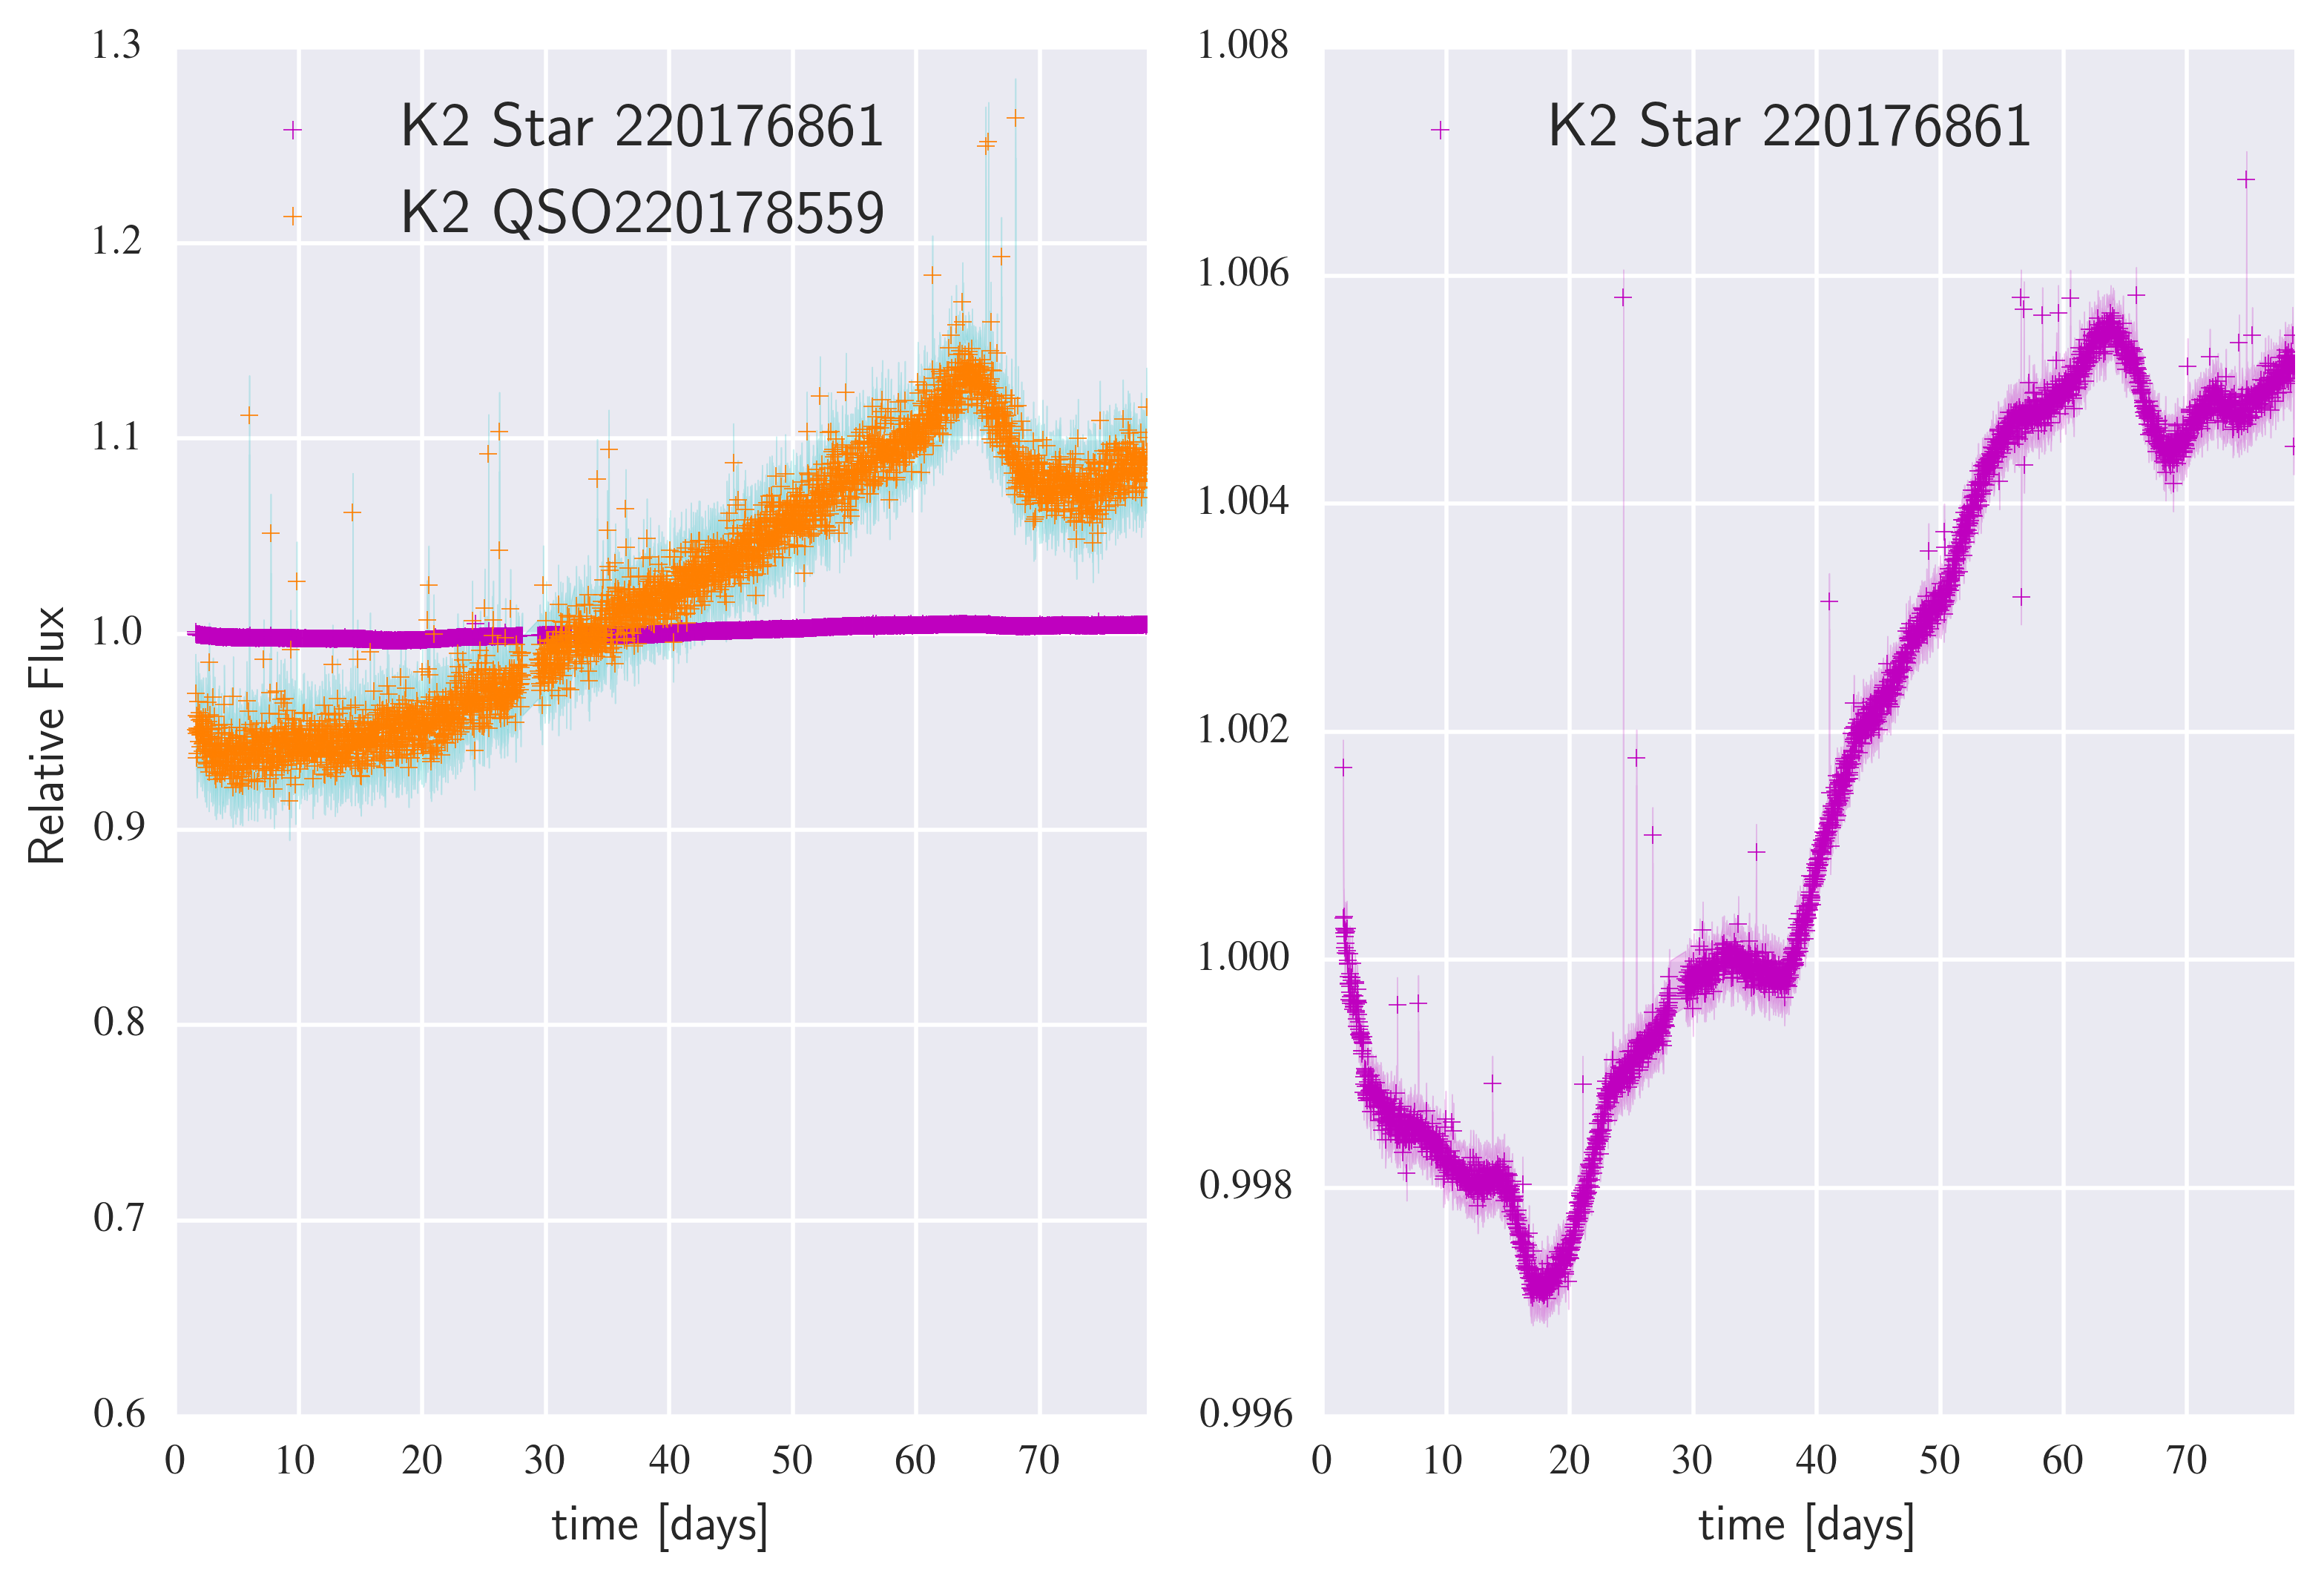
\includegraphics[width=\columnwidth]{220178559NearestNeighbor.png}
  	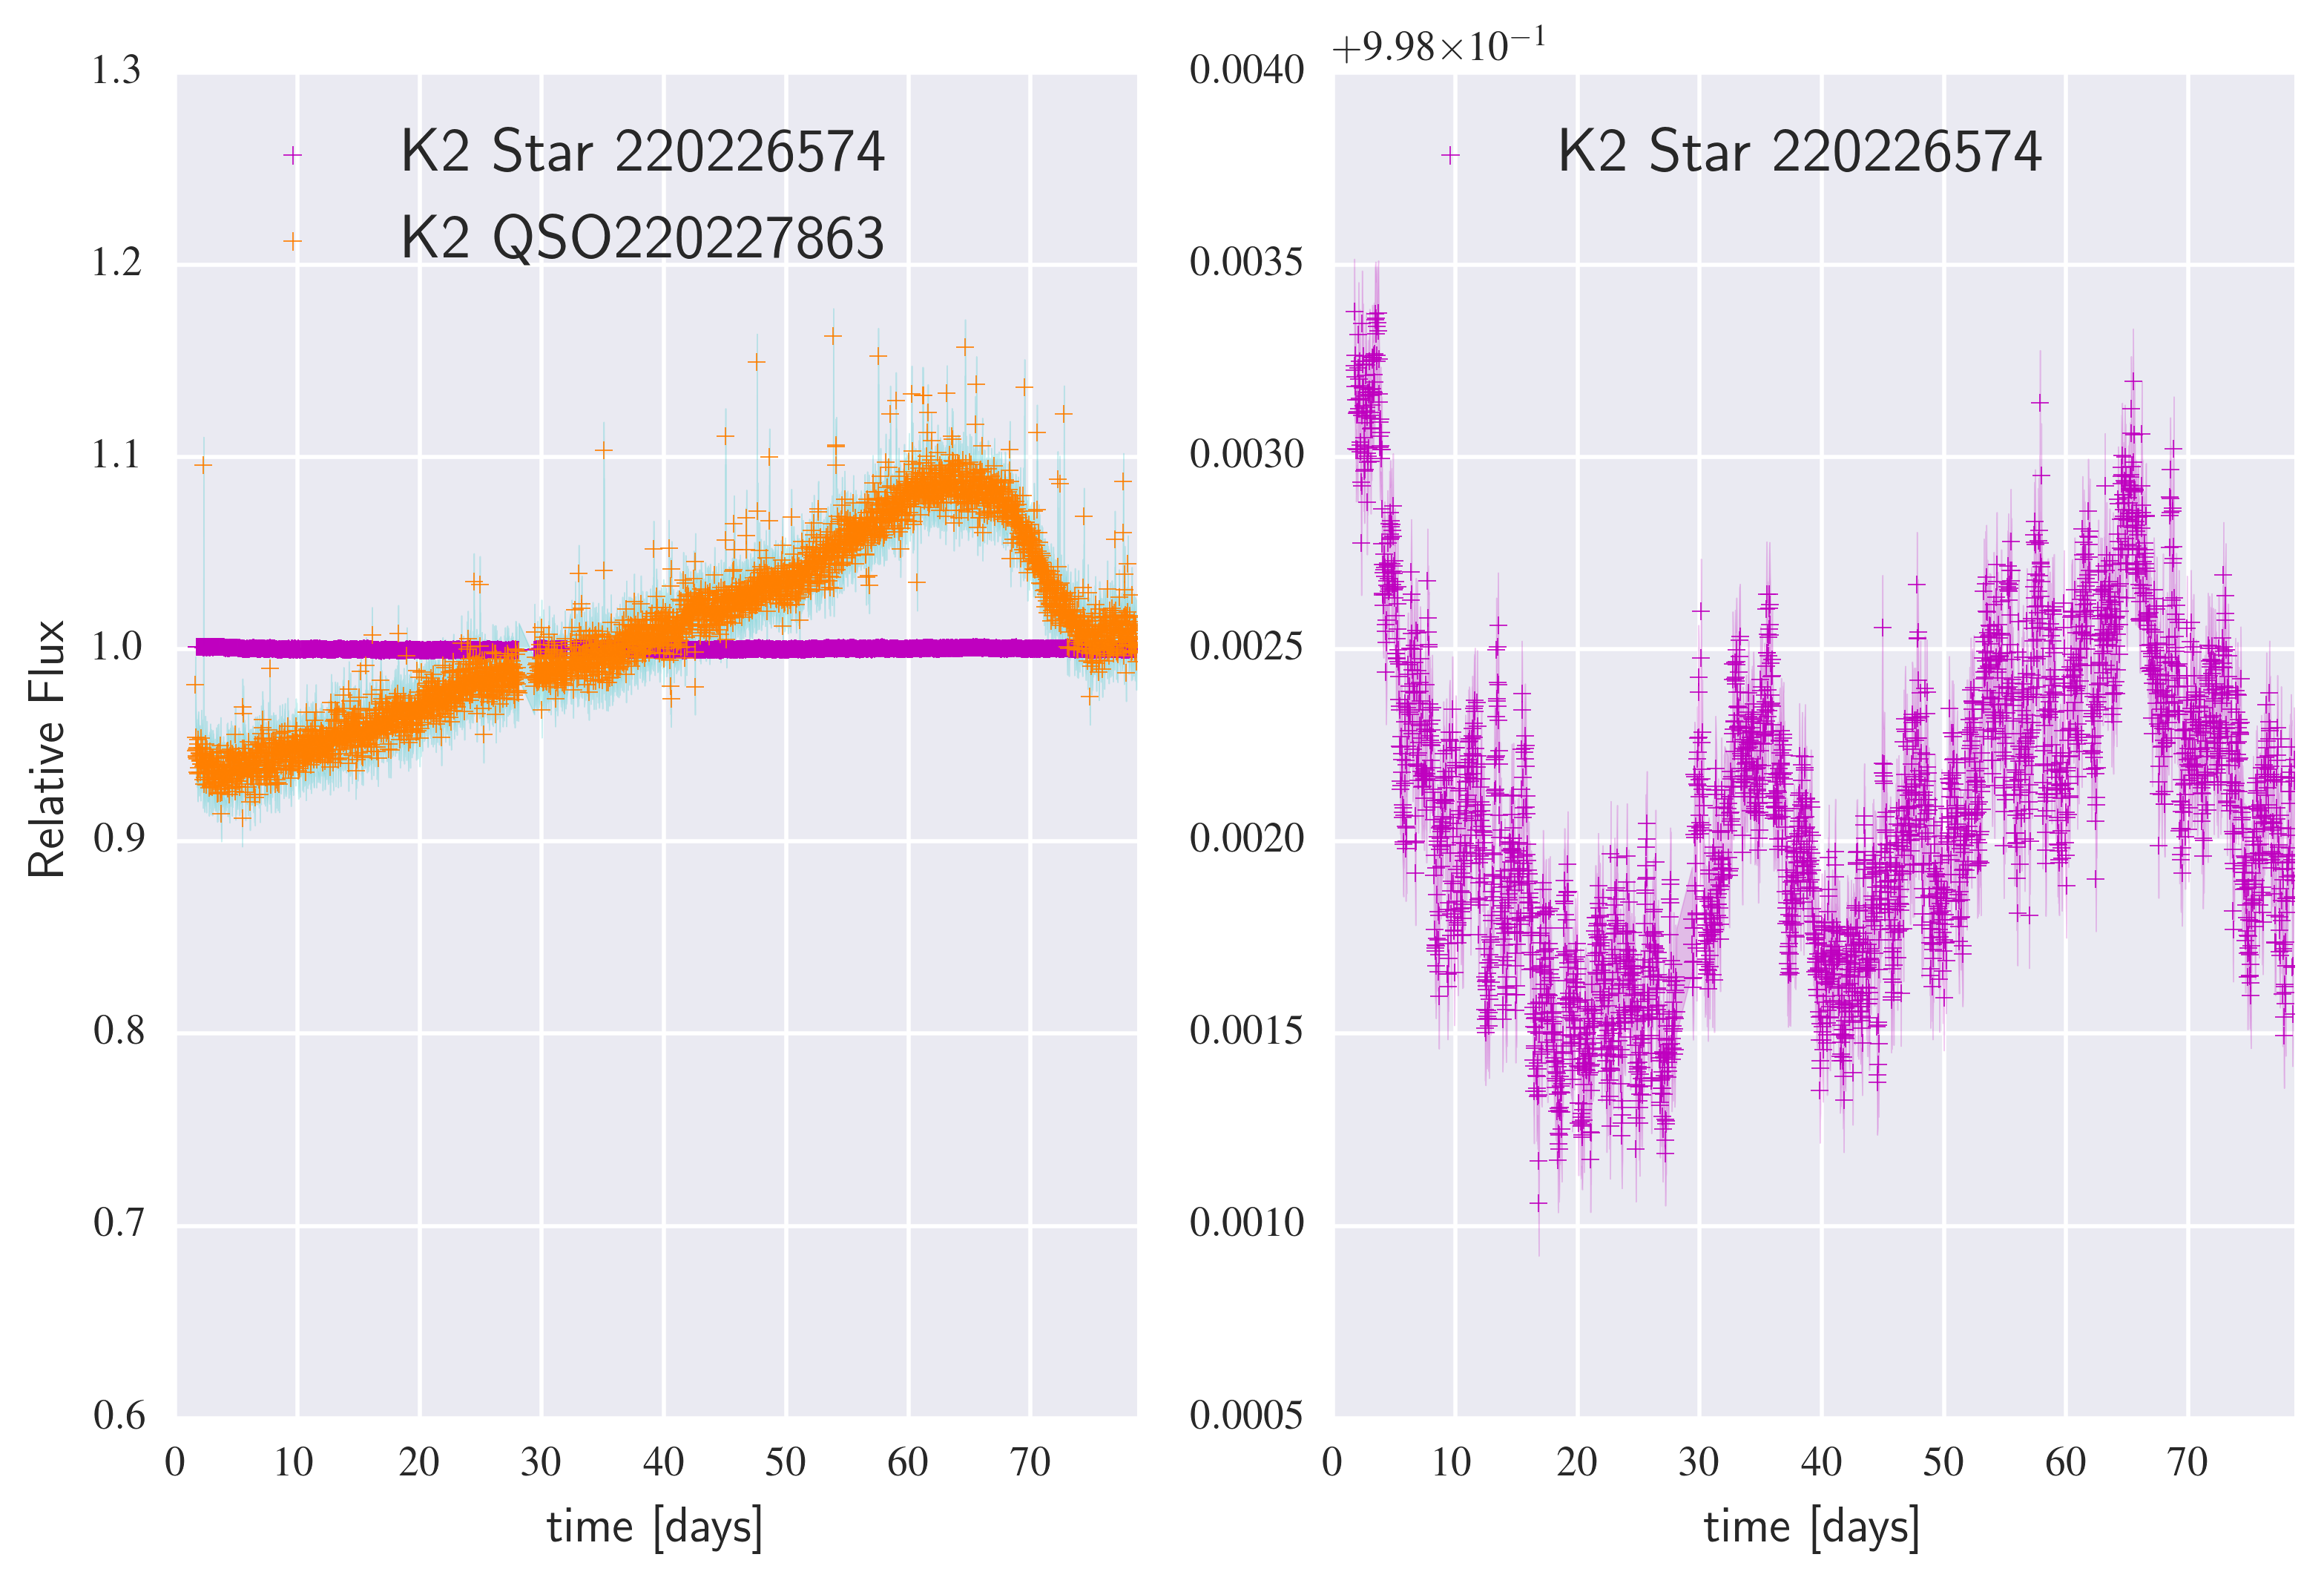
\includegraphics[width=\columnwidth]{220227863NearestNeighbor.png}
          	\caption{}
          	\label{fig:example_figure}
          \end{figure}

          \begin{figure}
          	% To include a figure from a file named example.*
          	% Allowable file formats are eps or ps if compiling using latex
          	% or pdf, png, jpg if compiling using pdflatex
 	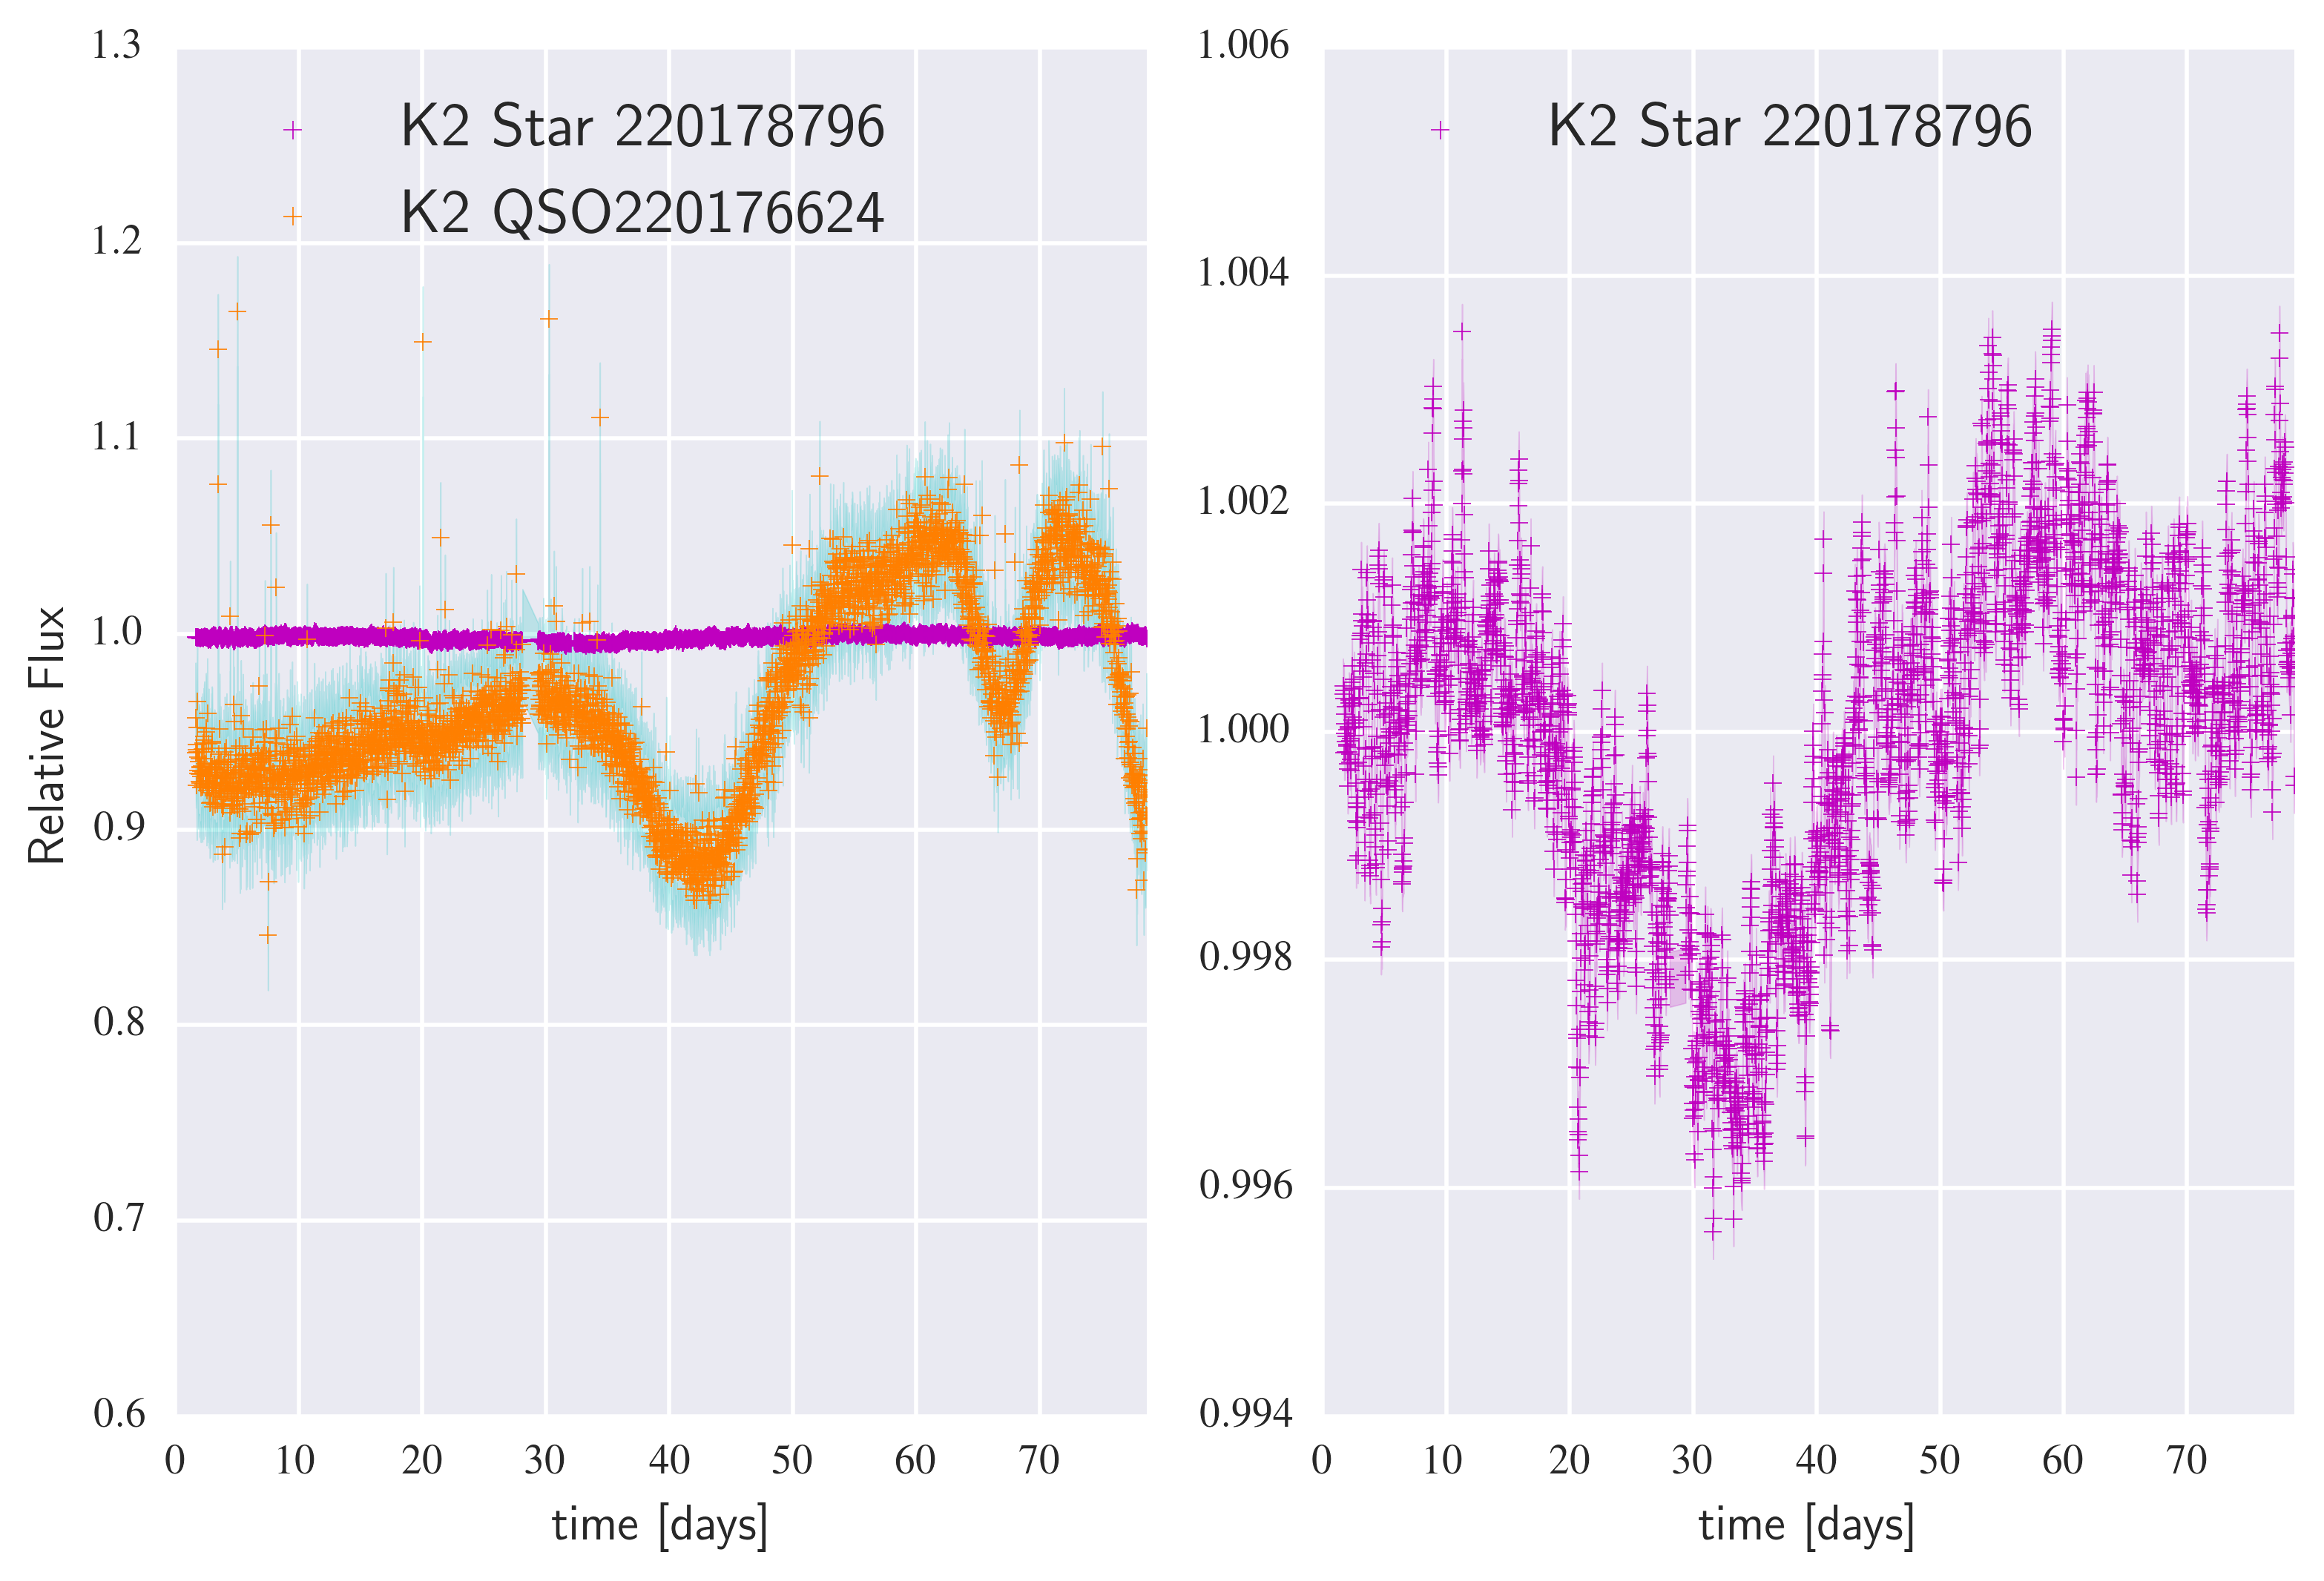
\includegraphics[width=\columnwidth]{220176624NearestNeighbor.png}
 	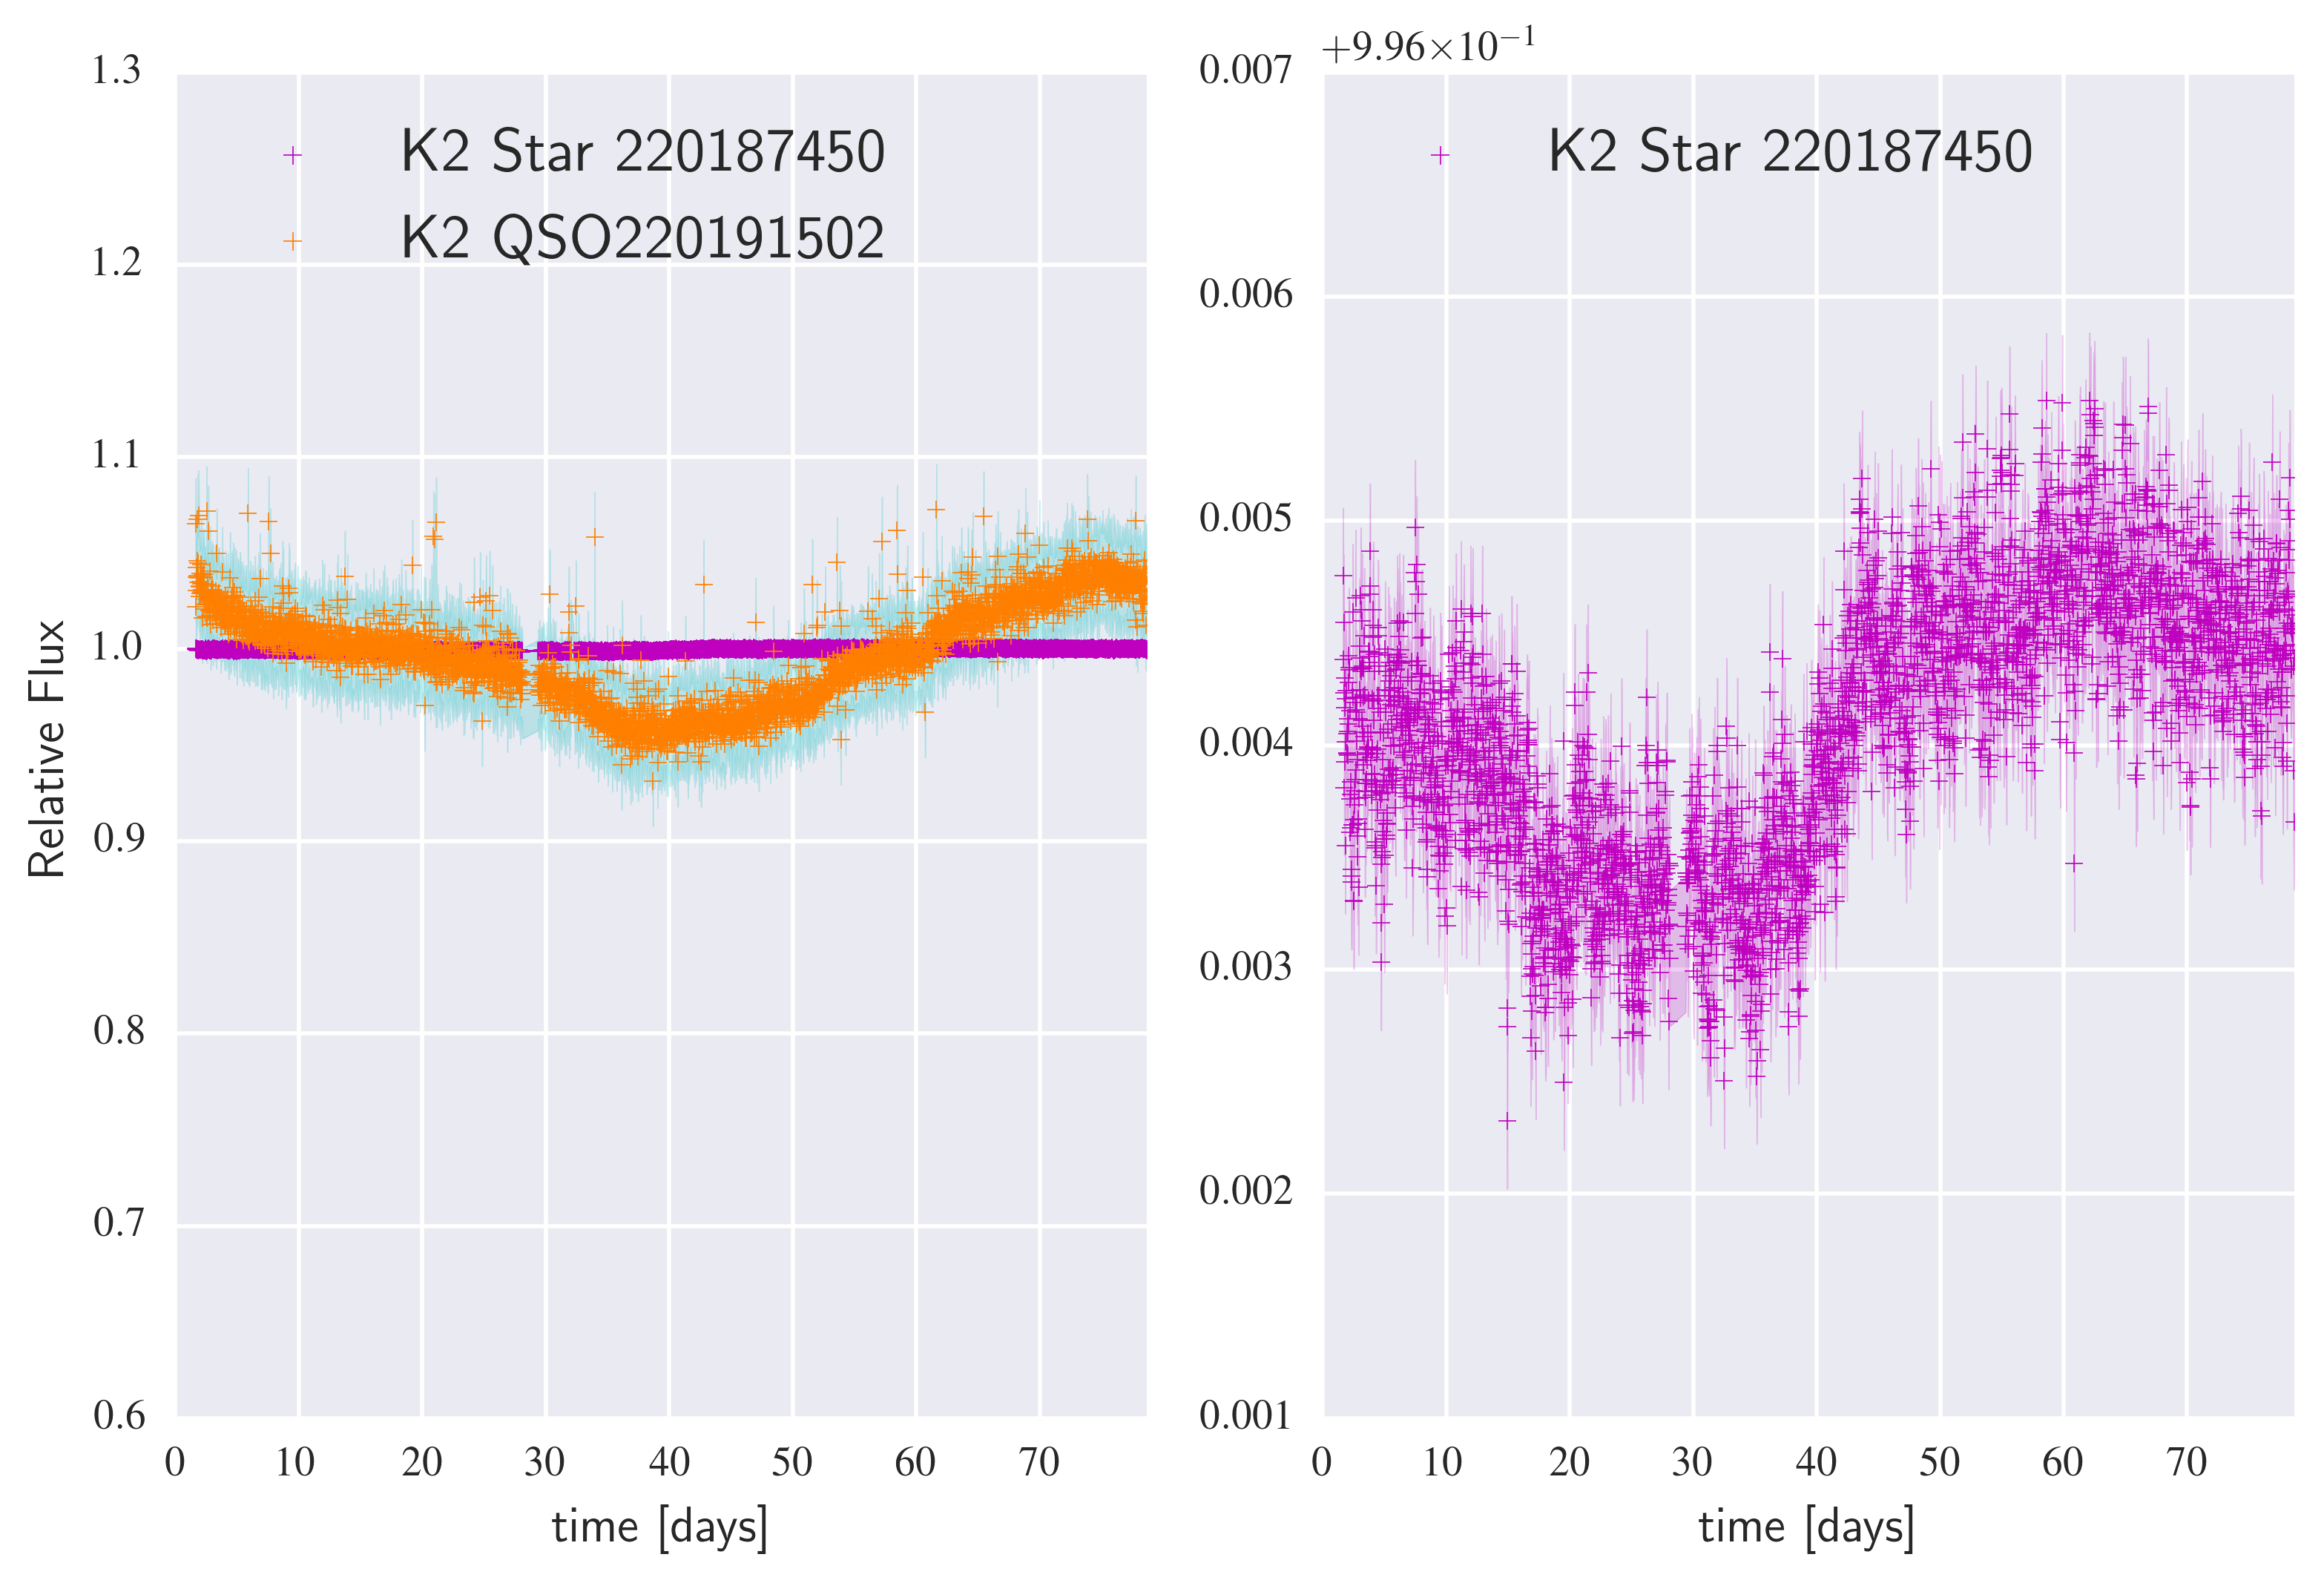
\includegraphics[width=\columnwidth]{220191502NearestNeighbor.png}
 	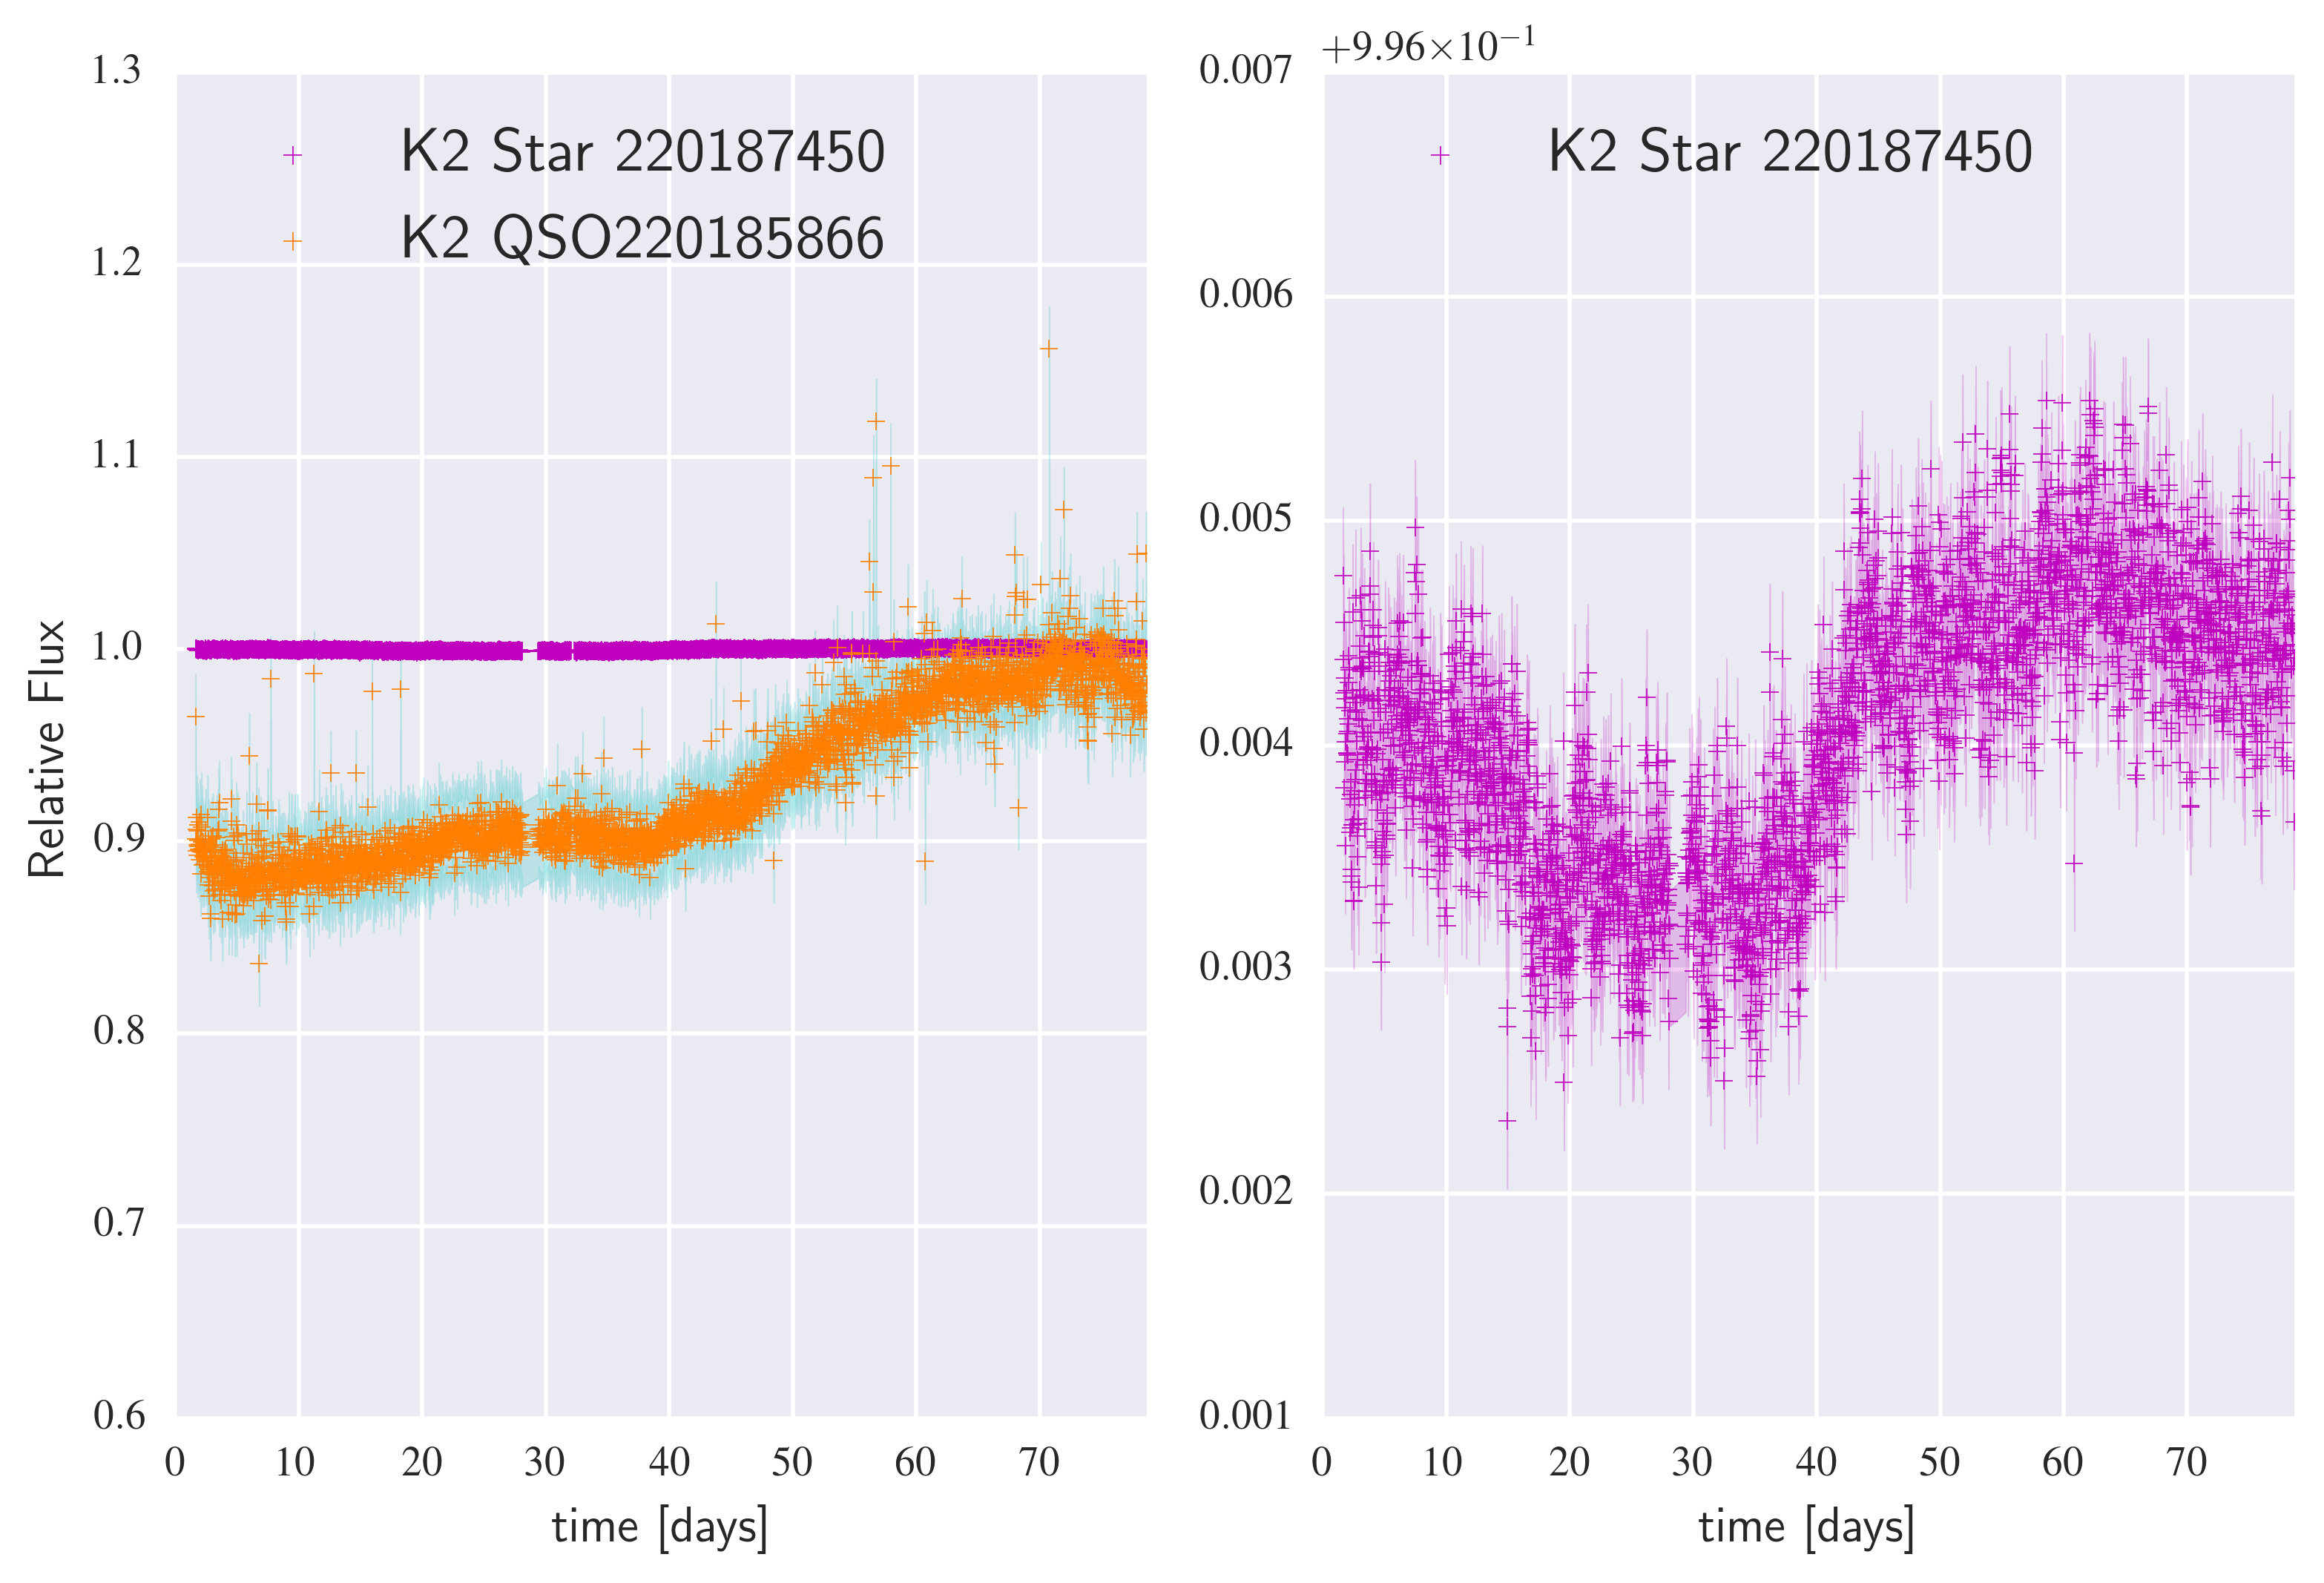
\includegraphics[width=\columnwidth]{220185866NearestNeighbor.png}
          	\caption{}
          	\label{fig:example_figure}
          \end{figure}          
          
          
       \begin{figure}
       	% To include a figure from a file named example.*
       	% Allowable file formats are eps or ps if compiling using latex
       	% or pdf, png, jpg if compiling using pdflatex
  	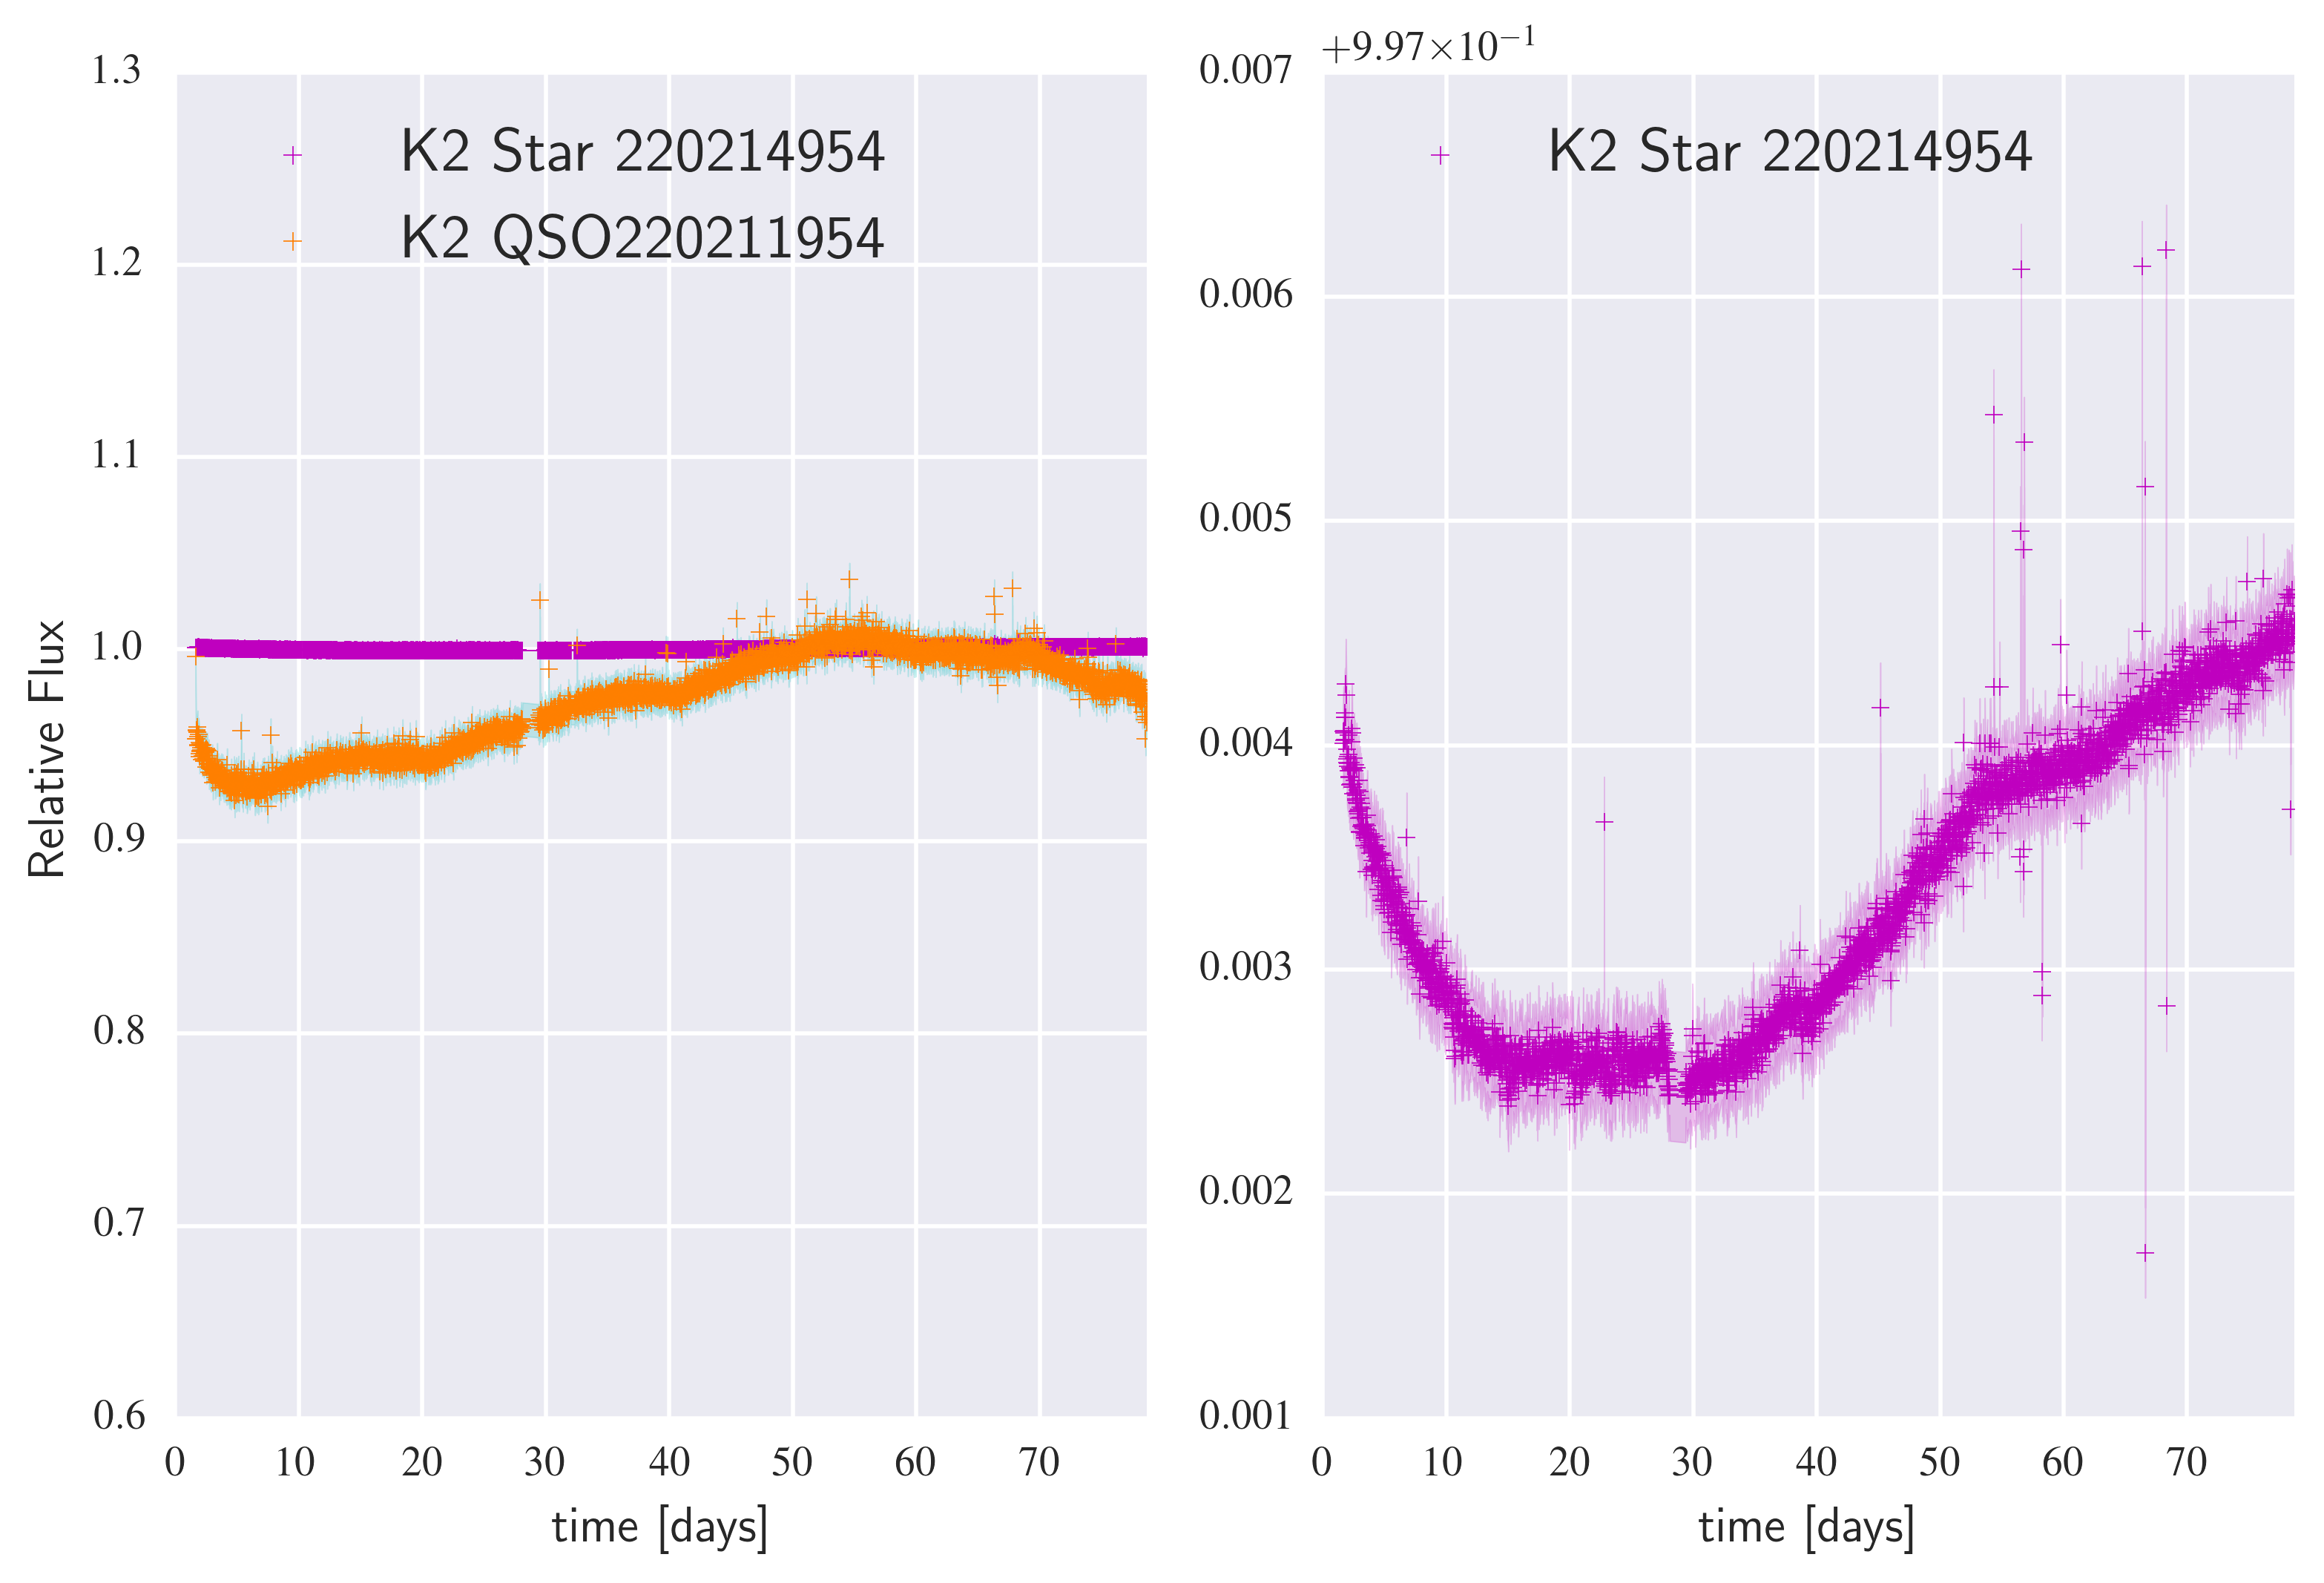
\includegraphics[width=\columnwidth]{220211954NearestNeighbor.png}
  	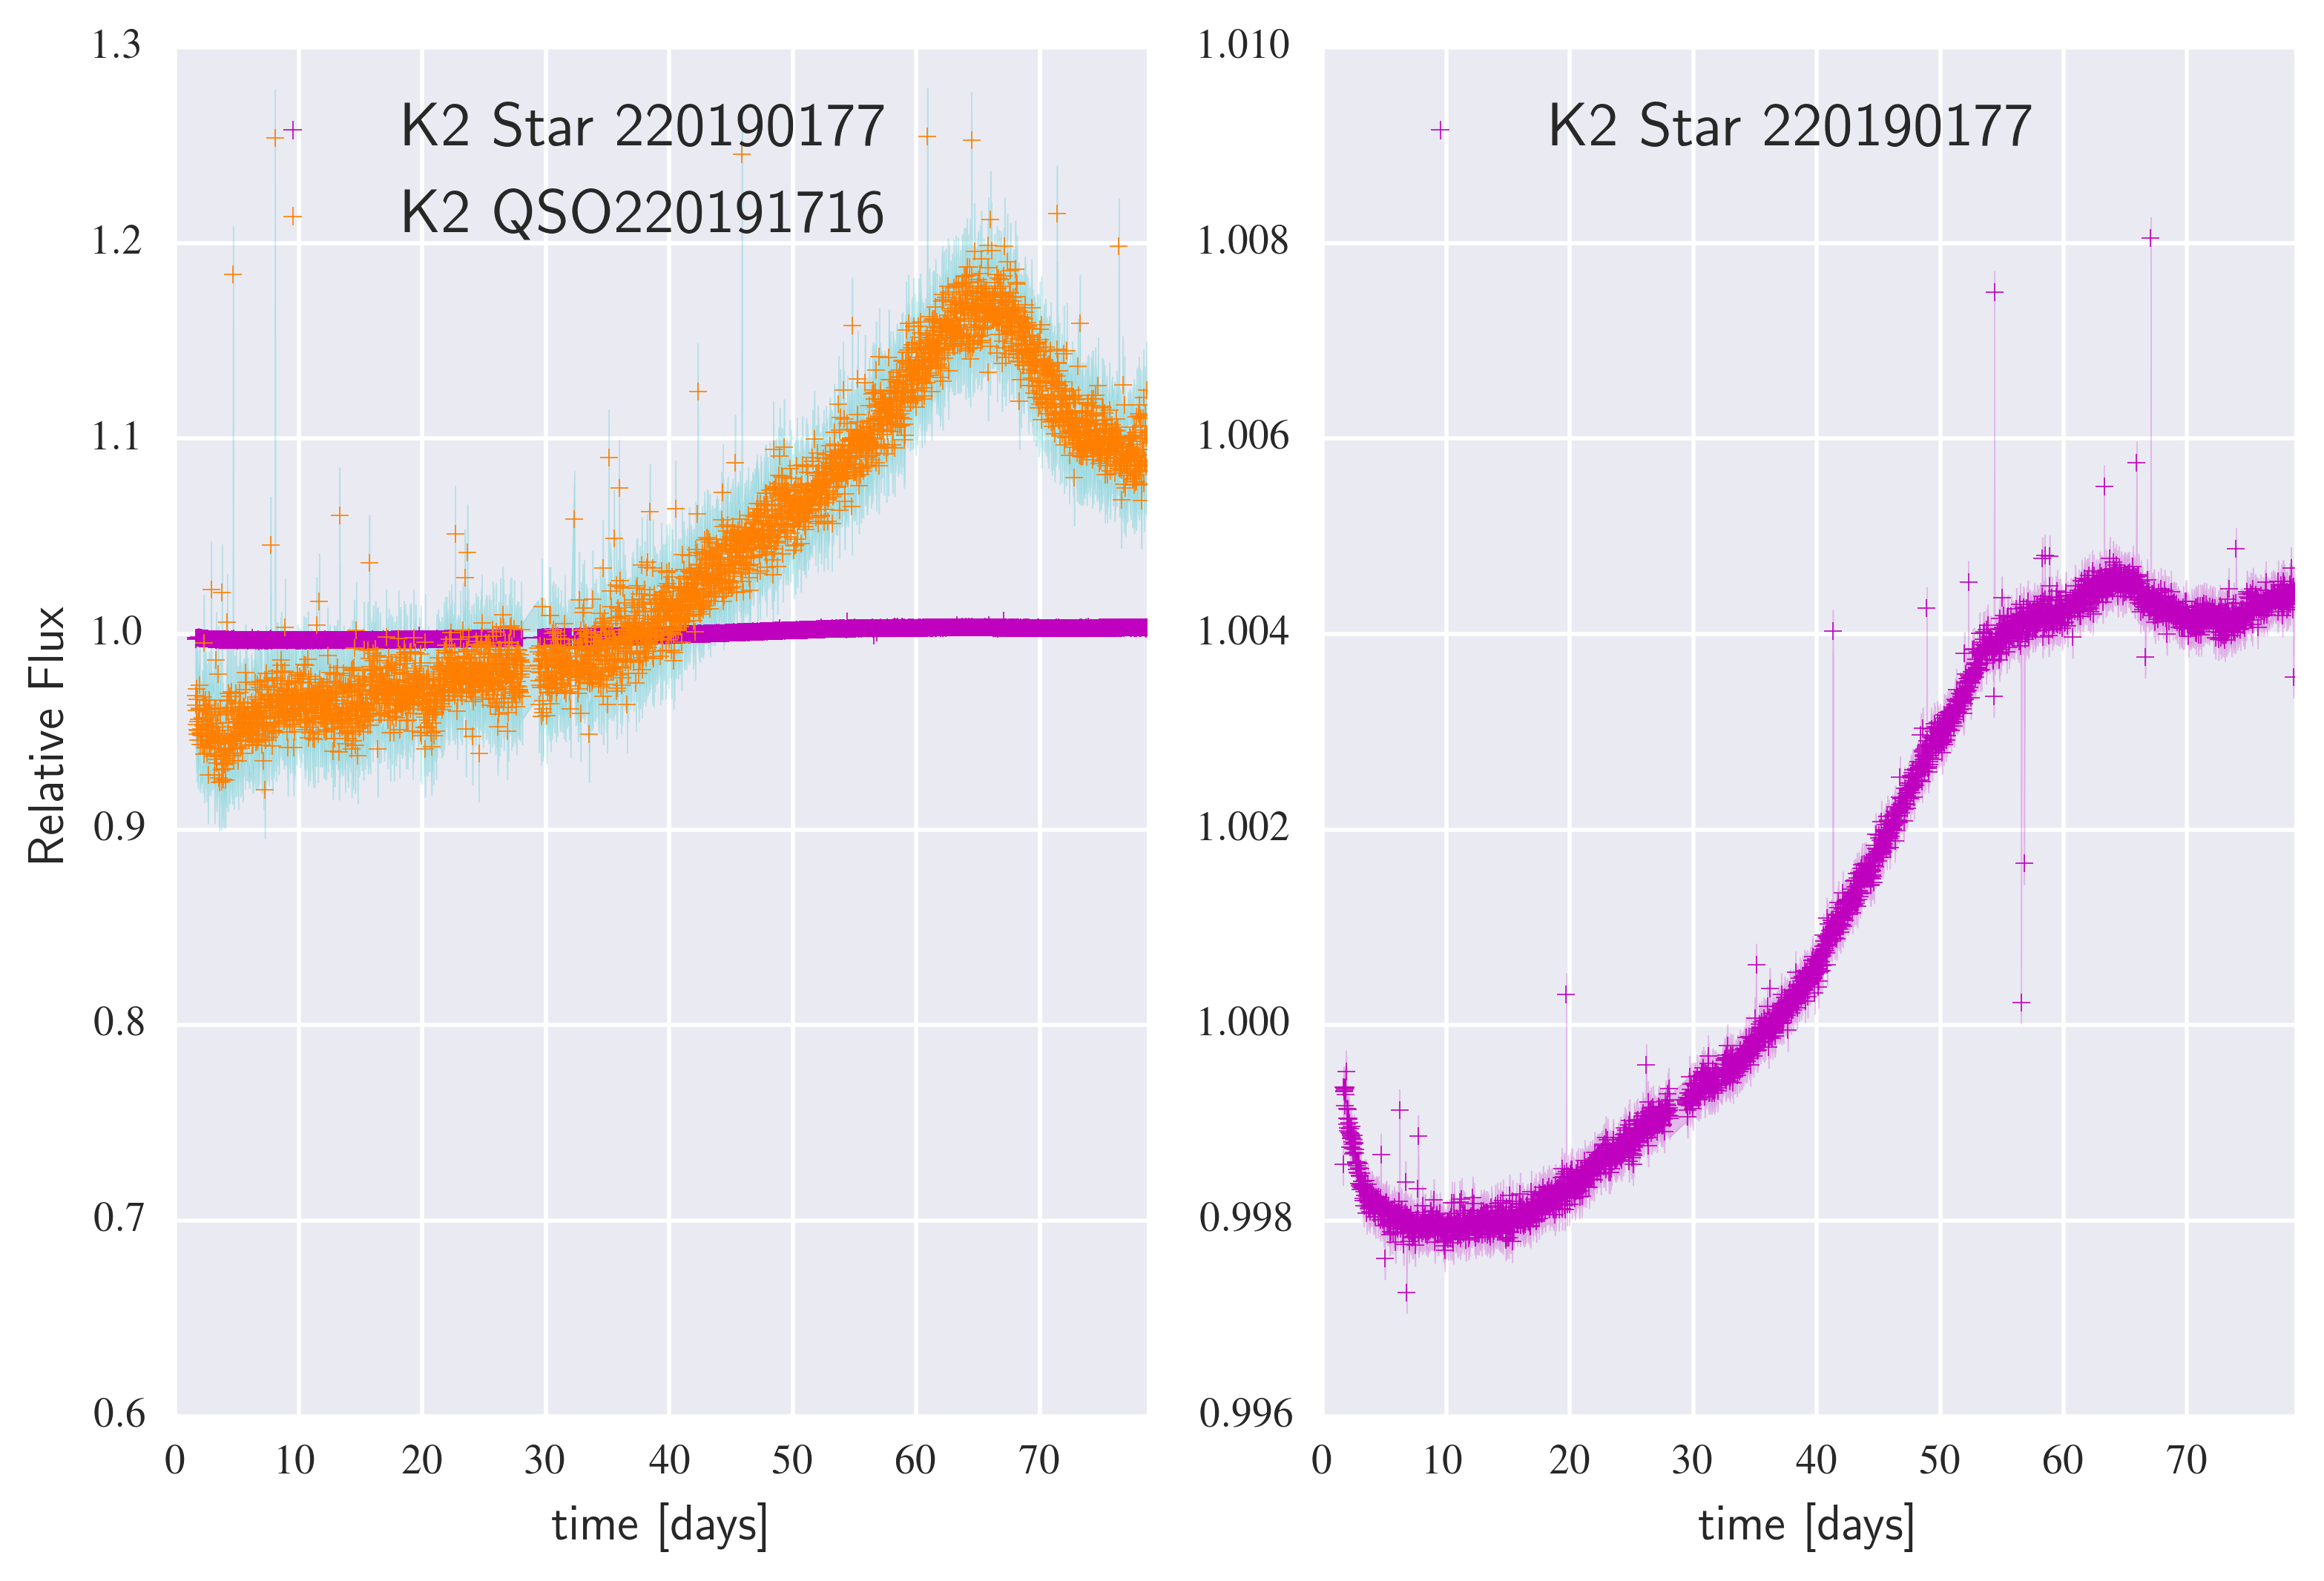
\includegraphics[width=\columnwidth]{220191716NearestNeighbor.png}
  	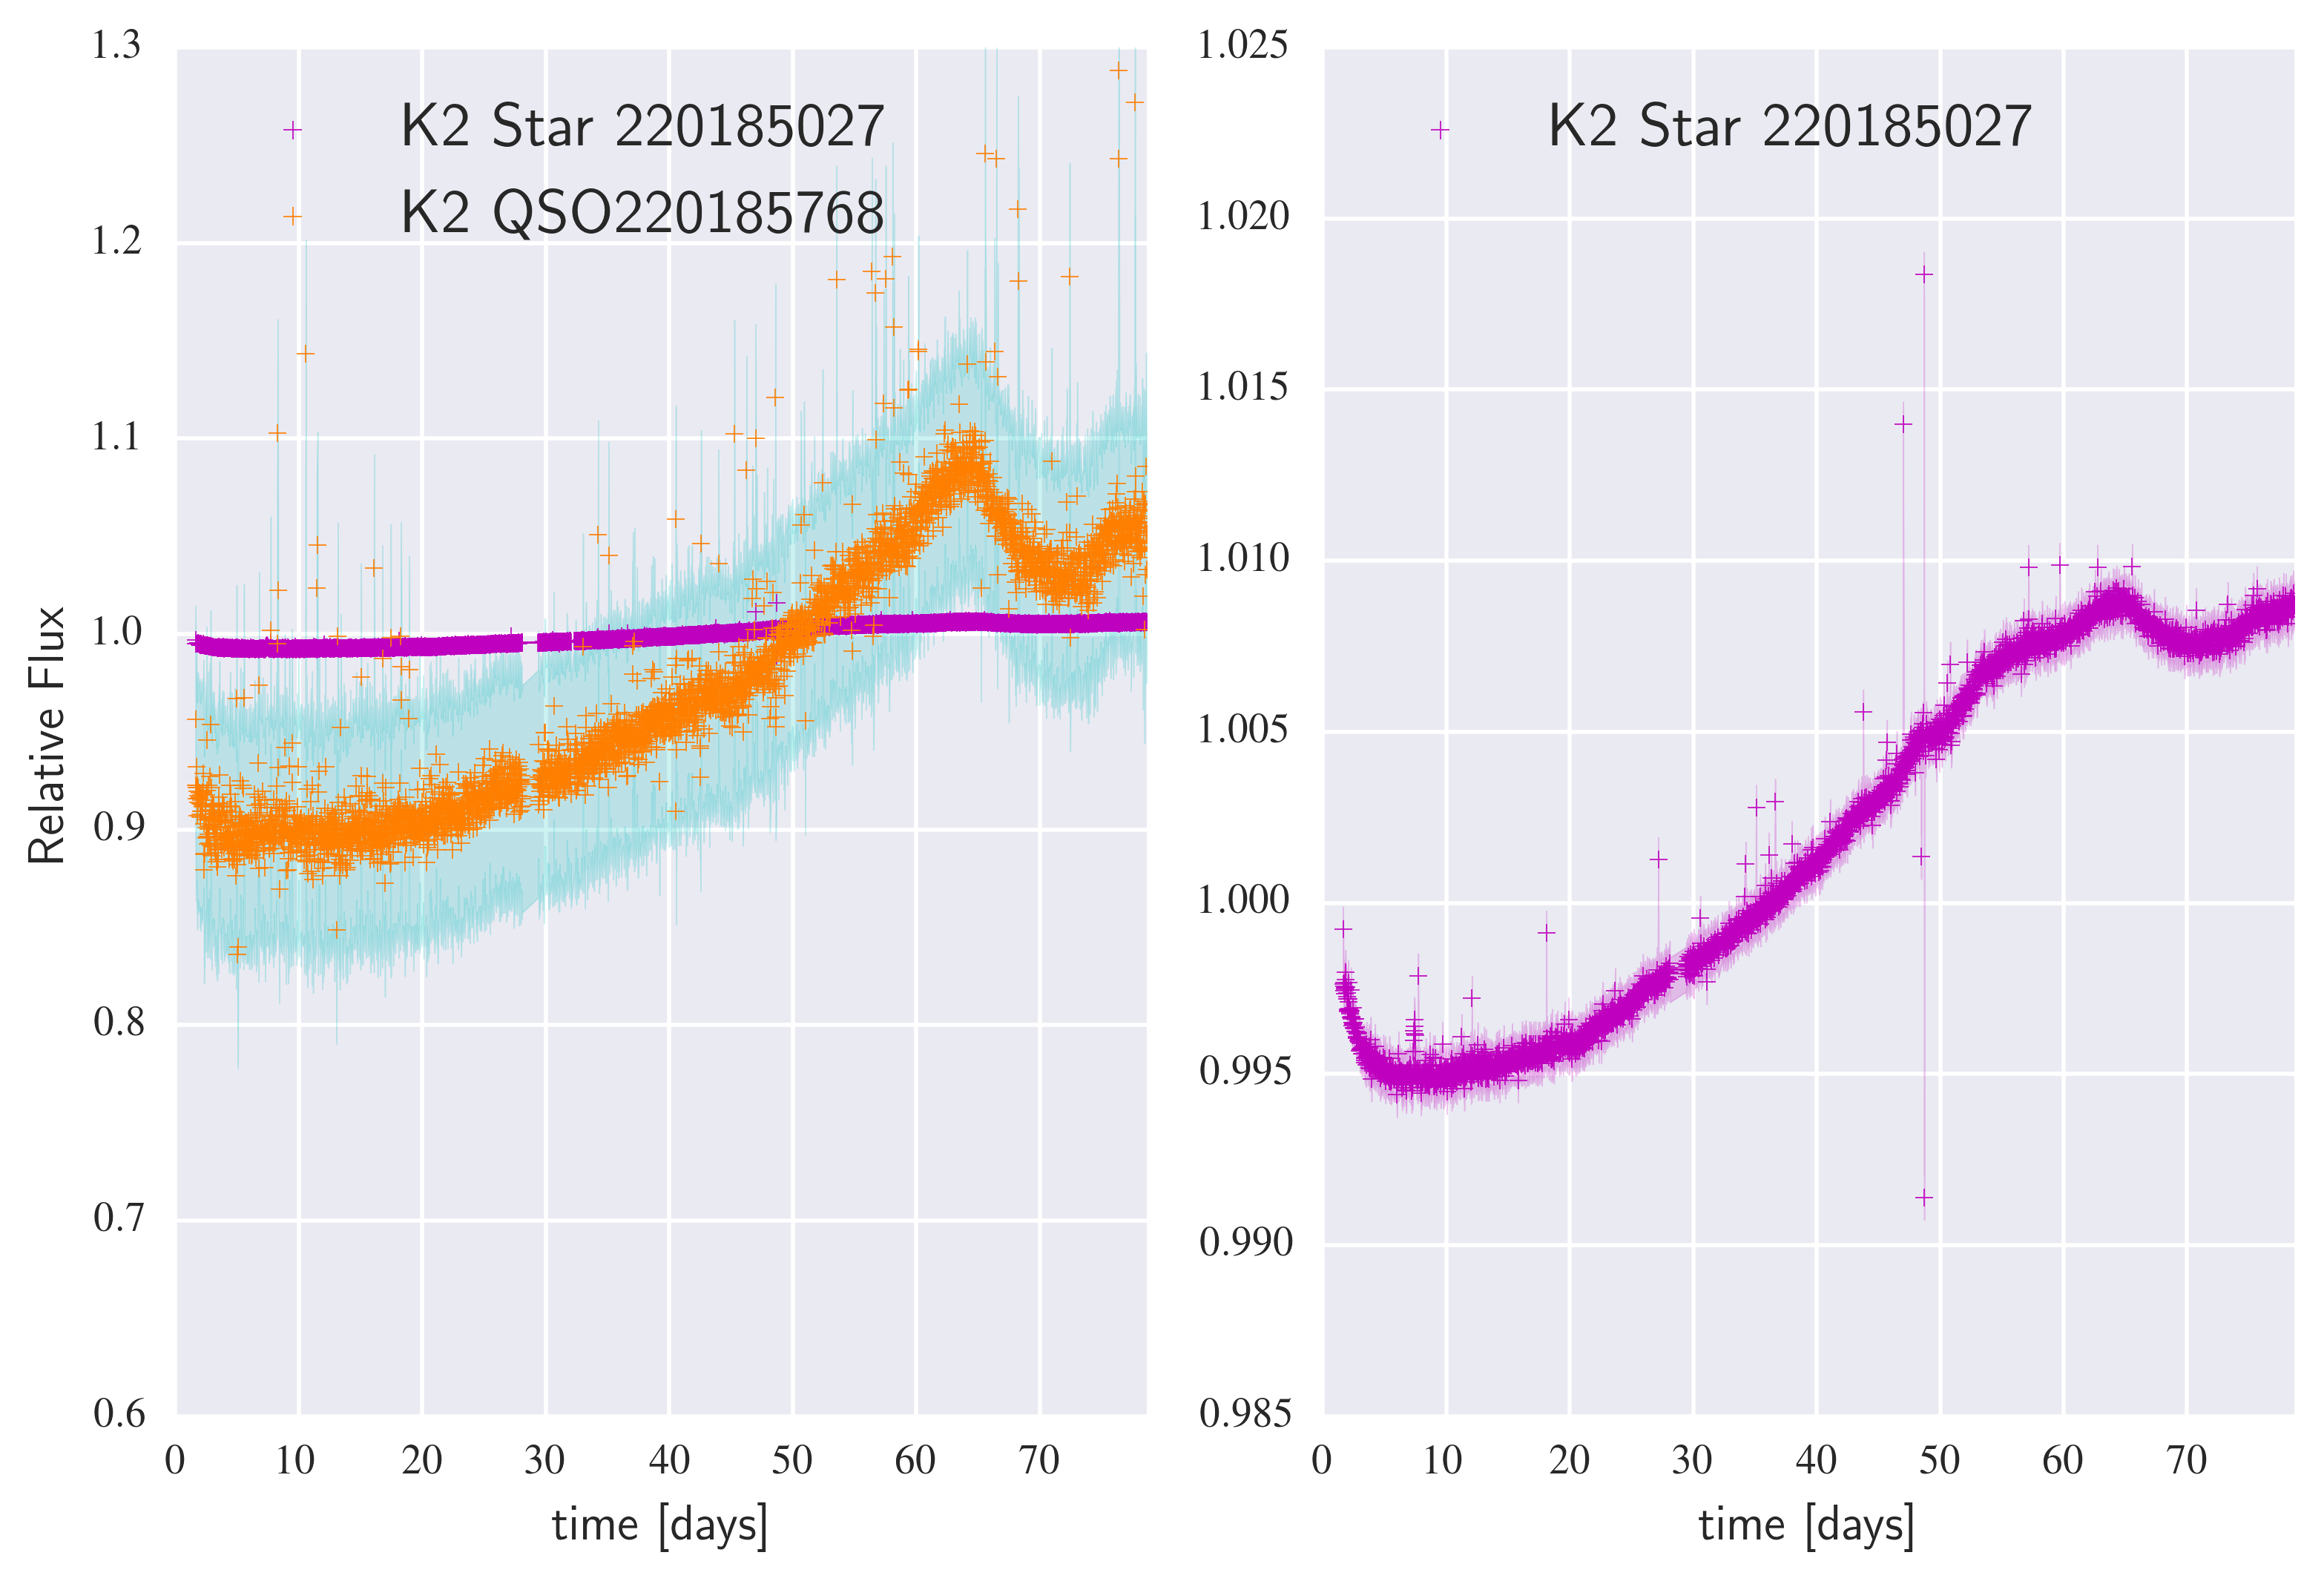
\includegraphics[width=\columnwidth]{220185768NearestNeighbor.png}
       	\caption{}
       	\label{fig:example_figure}
       \end{figure}                
          
          
       \begin{figure}
       	% To include a figure from a file named example.*
       	% Allowable file formats are eps or ps if compiling using latex
       	% or pdf, png, jpg if compiling using pdflatex
 	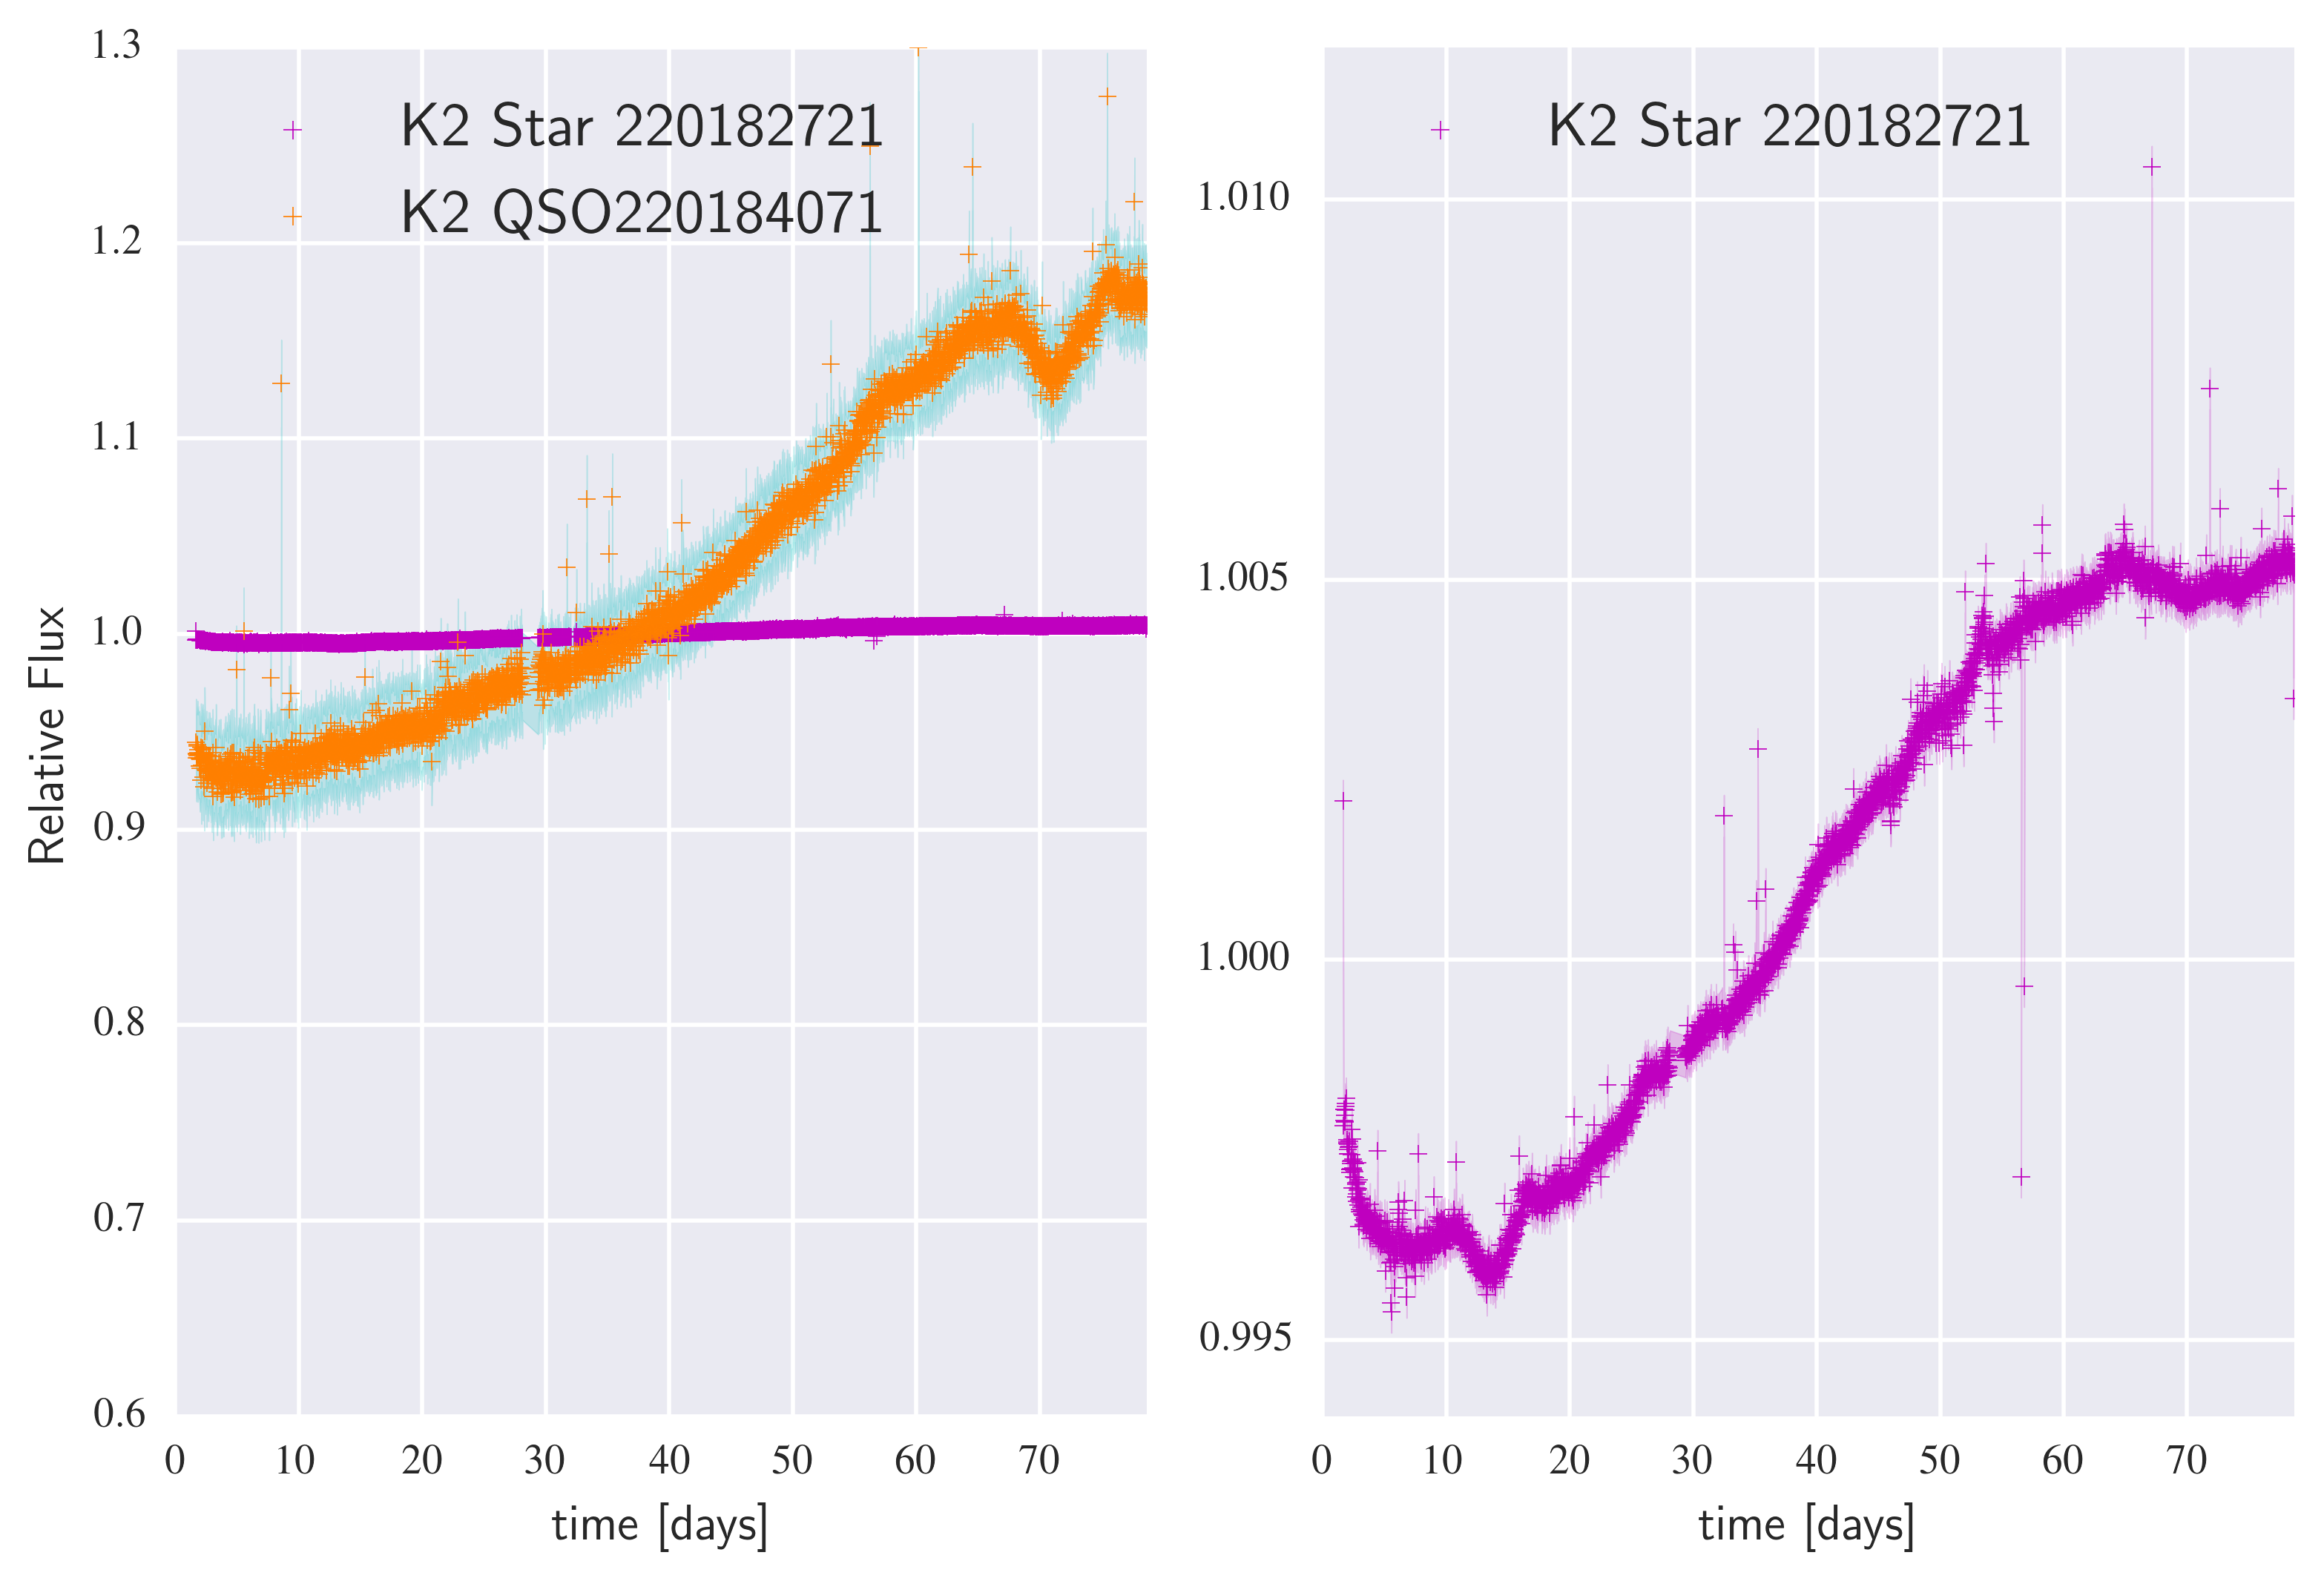
\includegraphics[width=\columnwidth]{220184071NearestNeighbor.png}
 	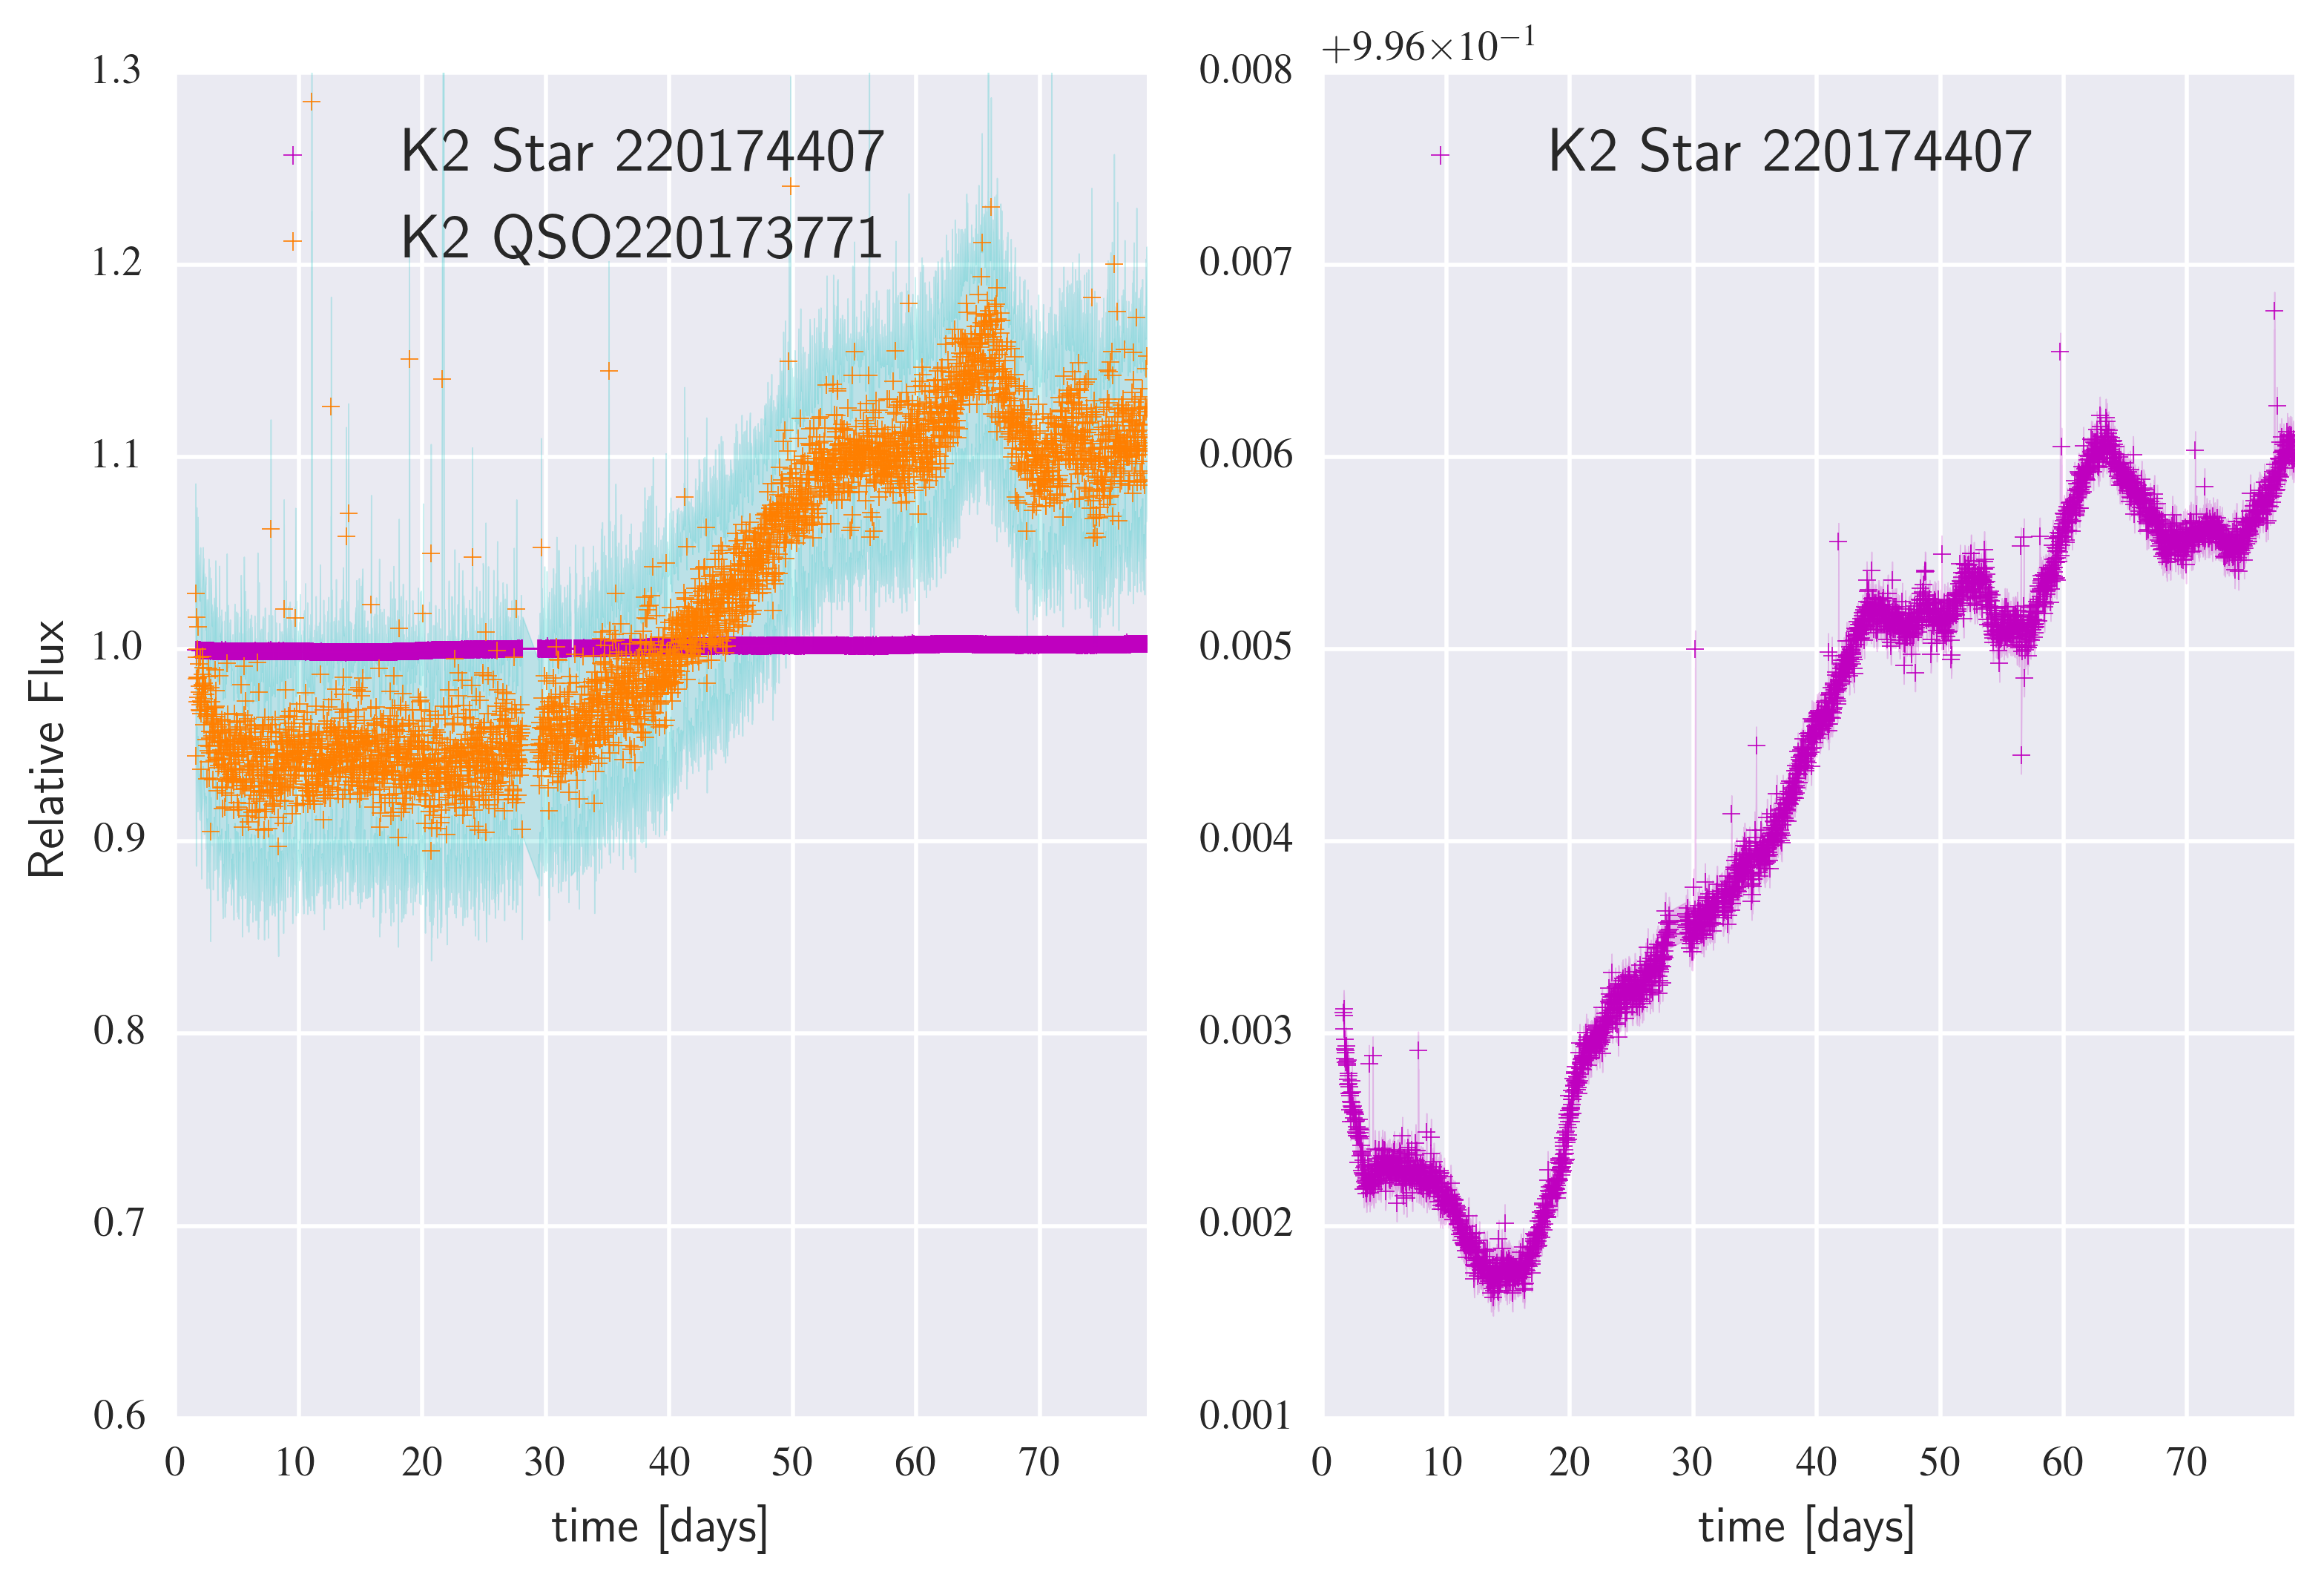
\includegraphics[width=\columnwidth]{220173771NearestNeighbor.png}
 	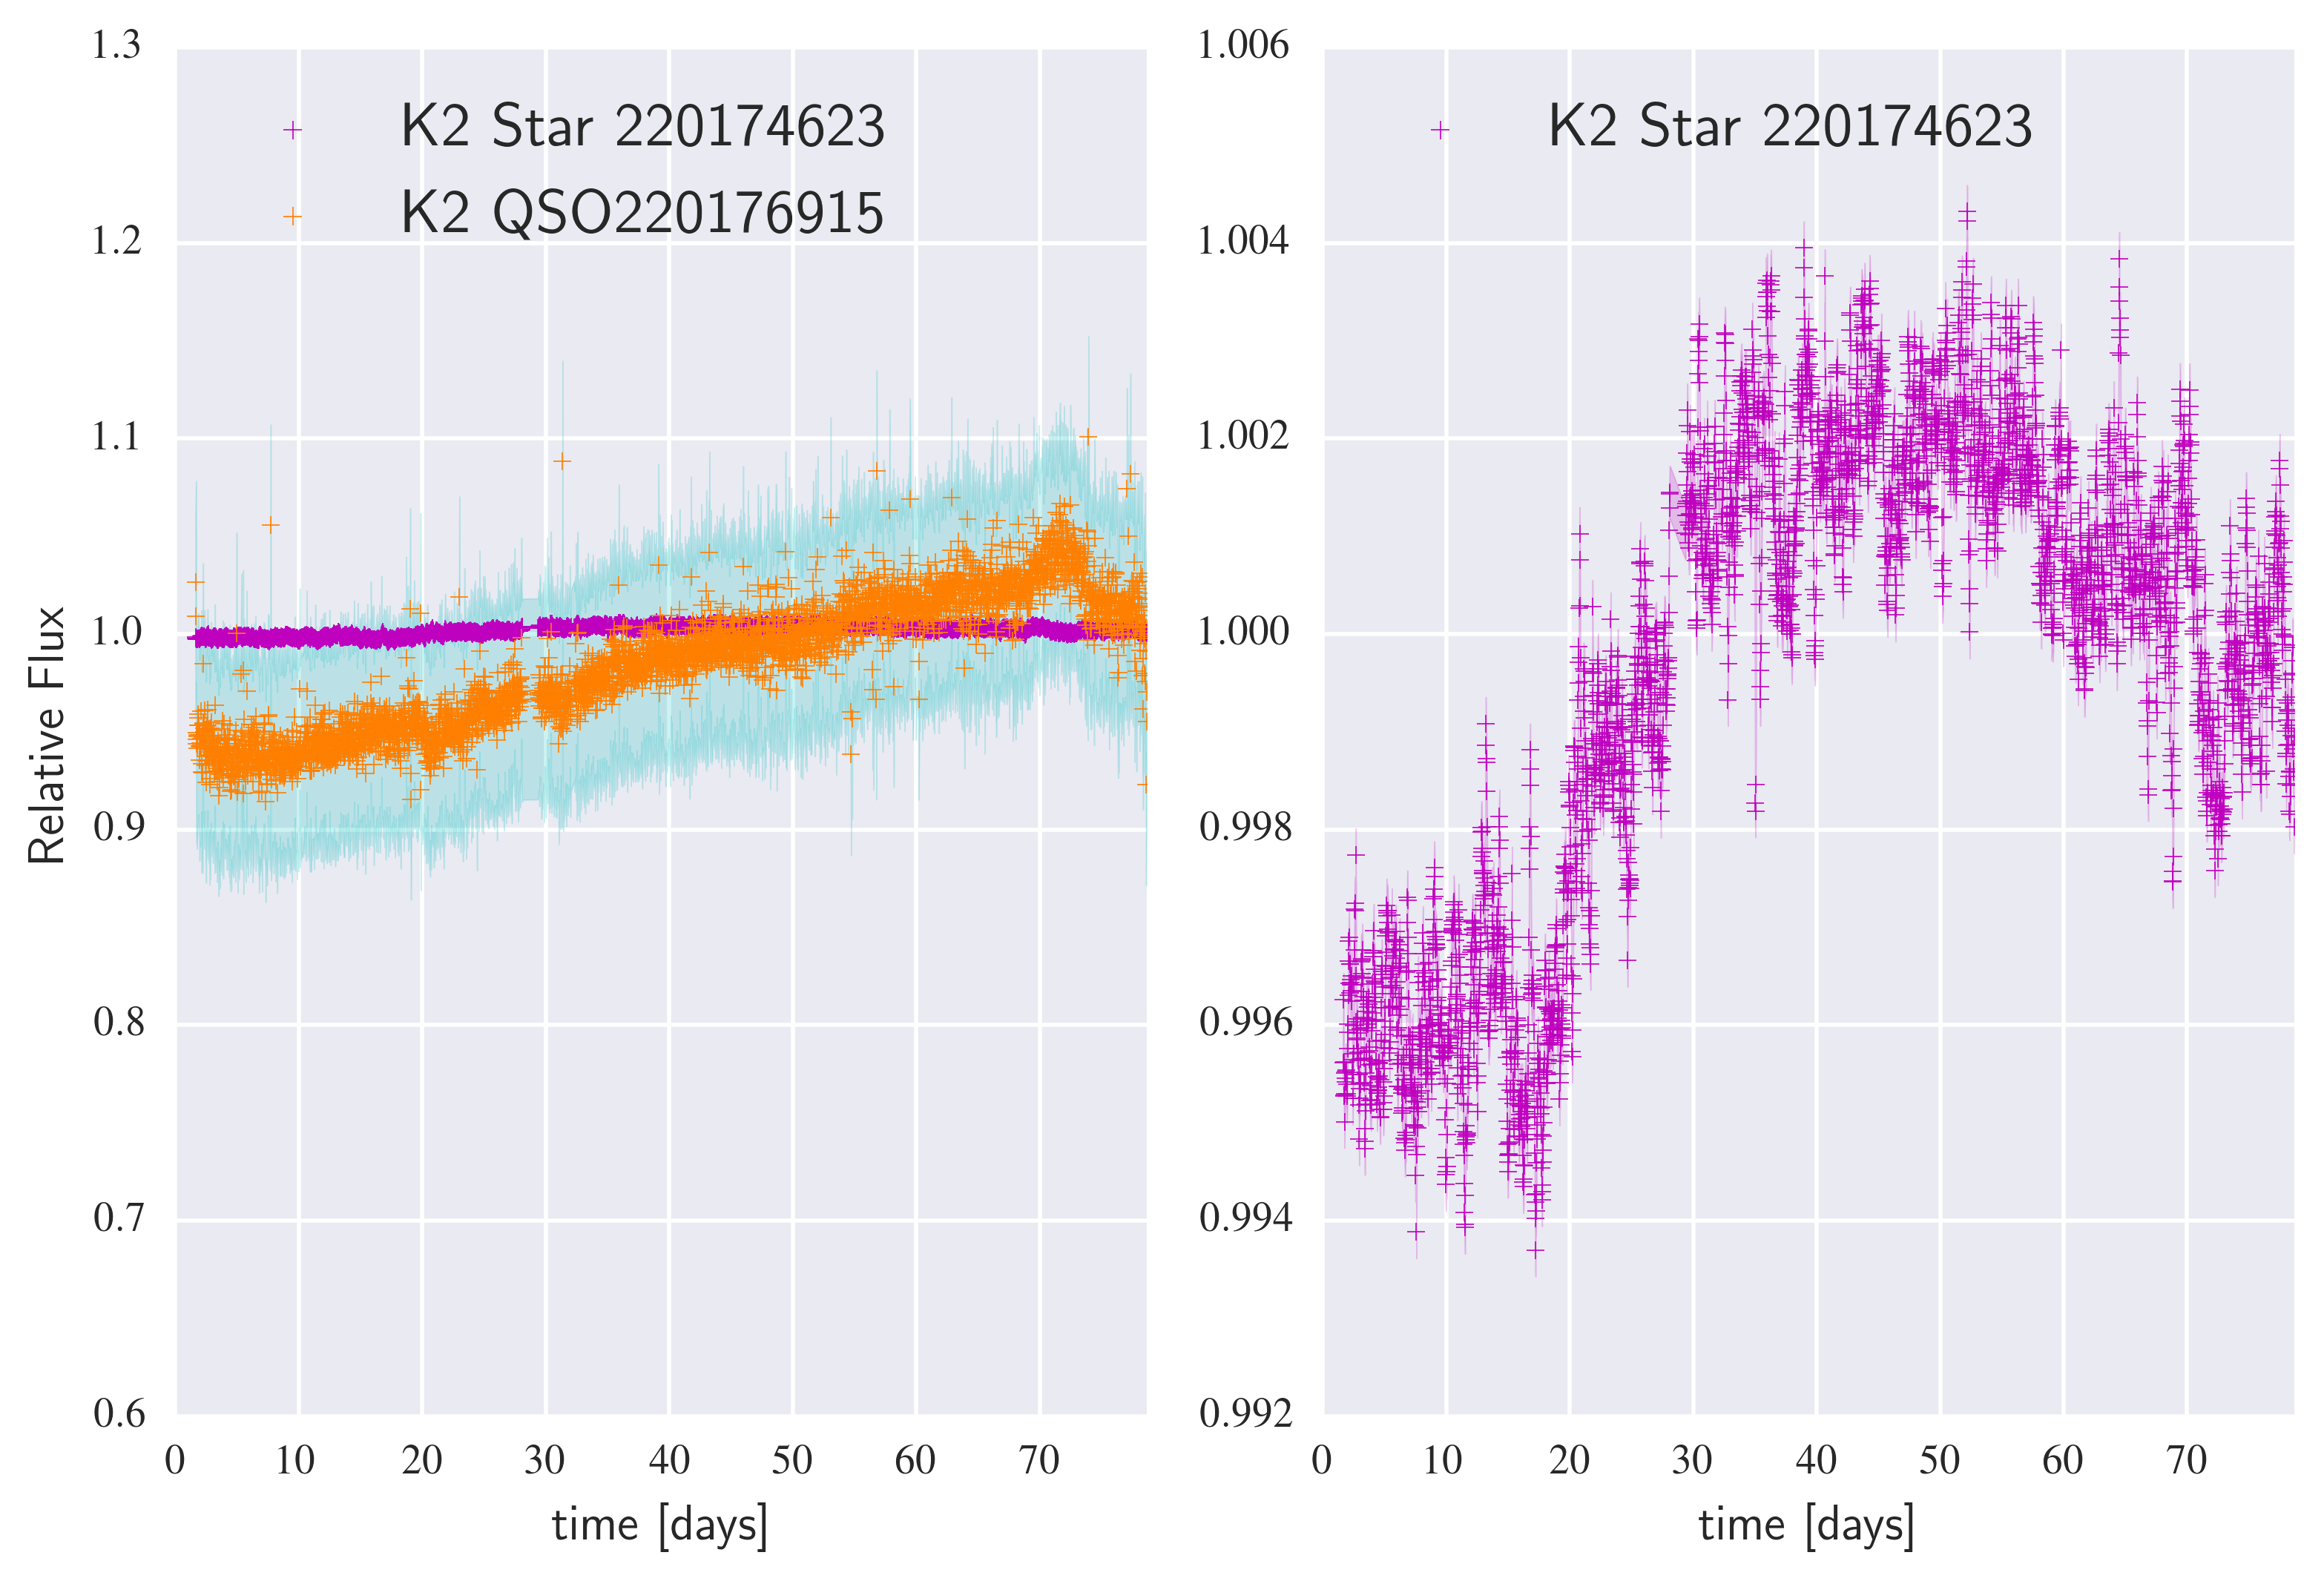
\includegraphics[width=\columnwidth]{220176915NearestNeighbor.png}
       	\caption{}
       	\label{fig:example_figure}
       \end{figure}      

        \begin{figure}
        	% To include a figure from a file named example.*
        	% Allowable file formats are eps or ps if compiling using latex
        	% or pdf, png, jpg if compiling using pdflatex
 	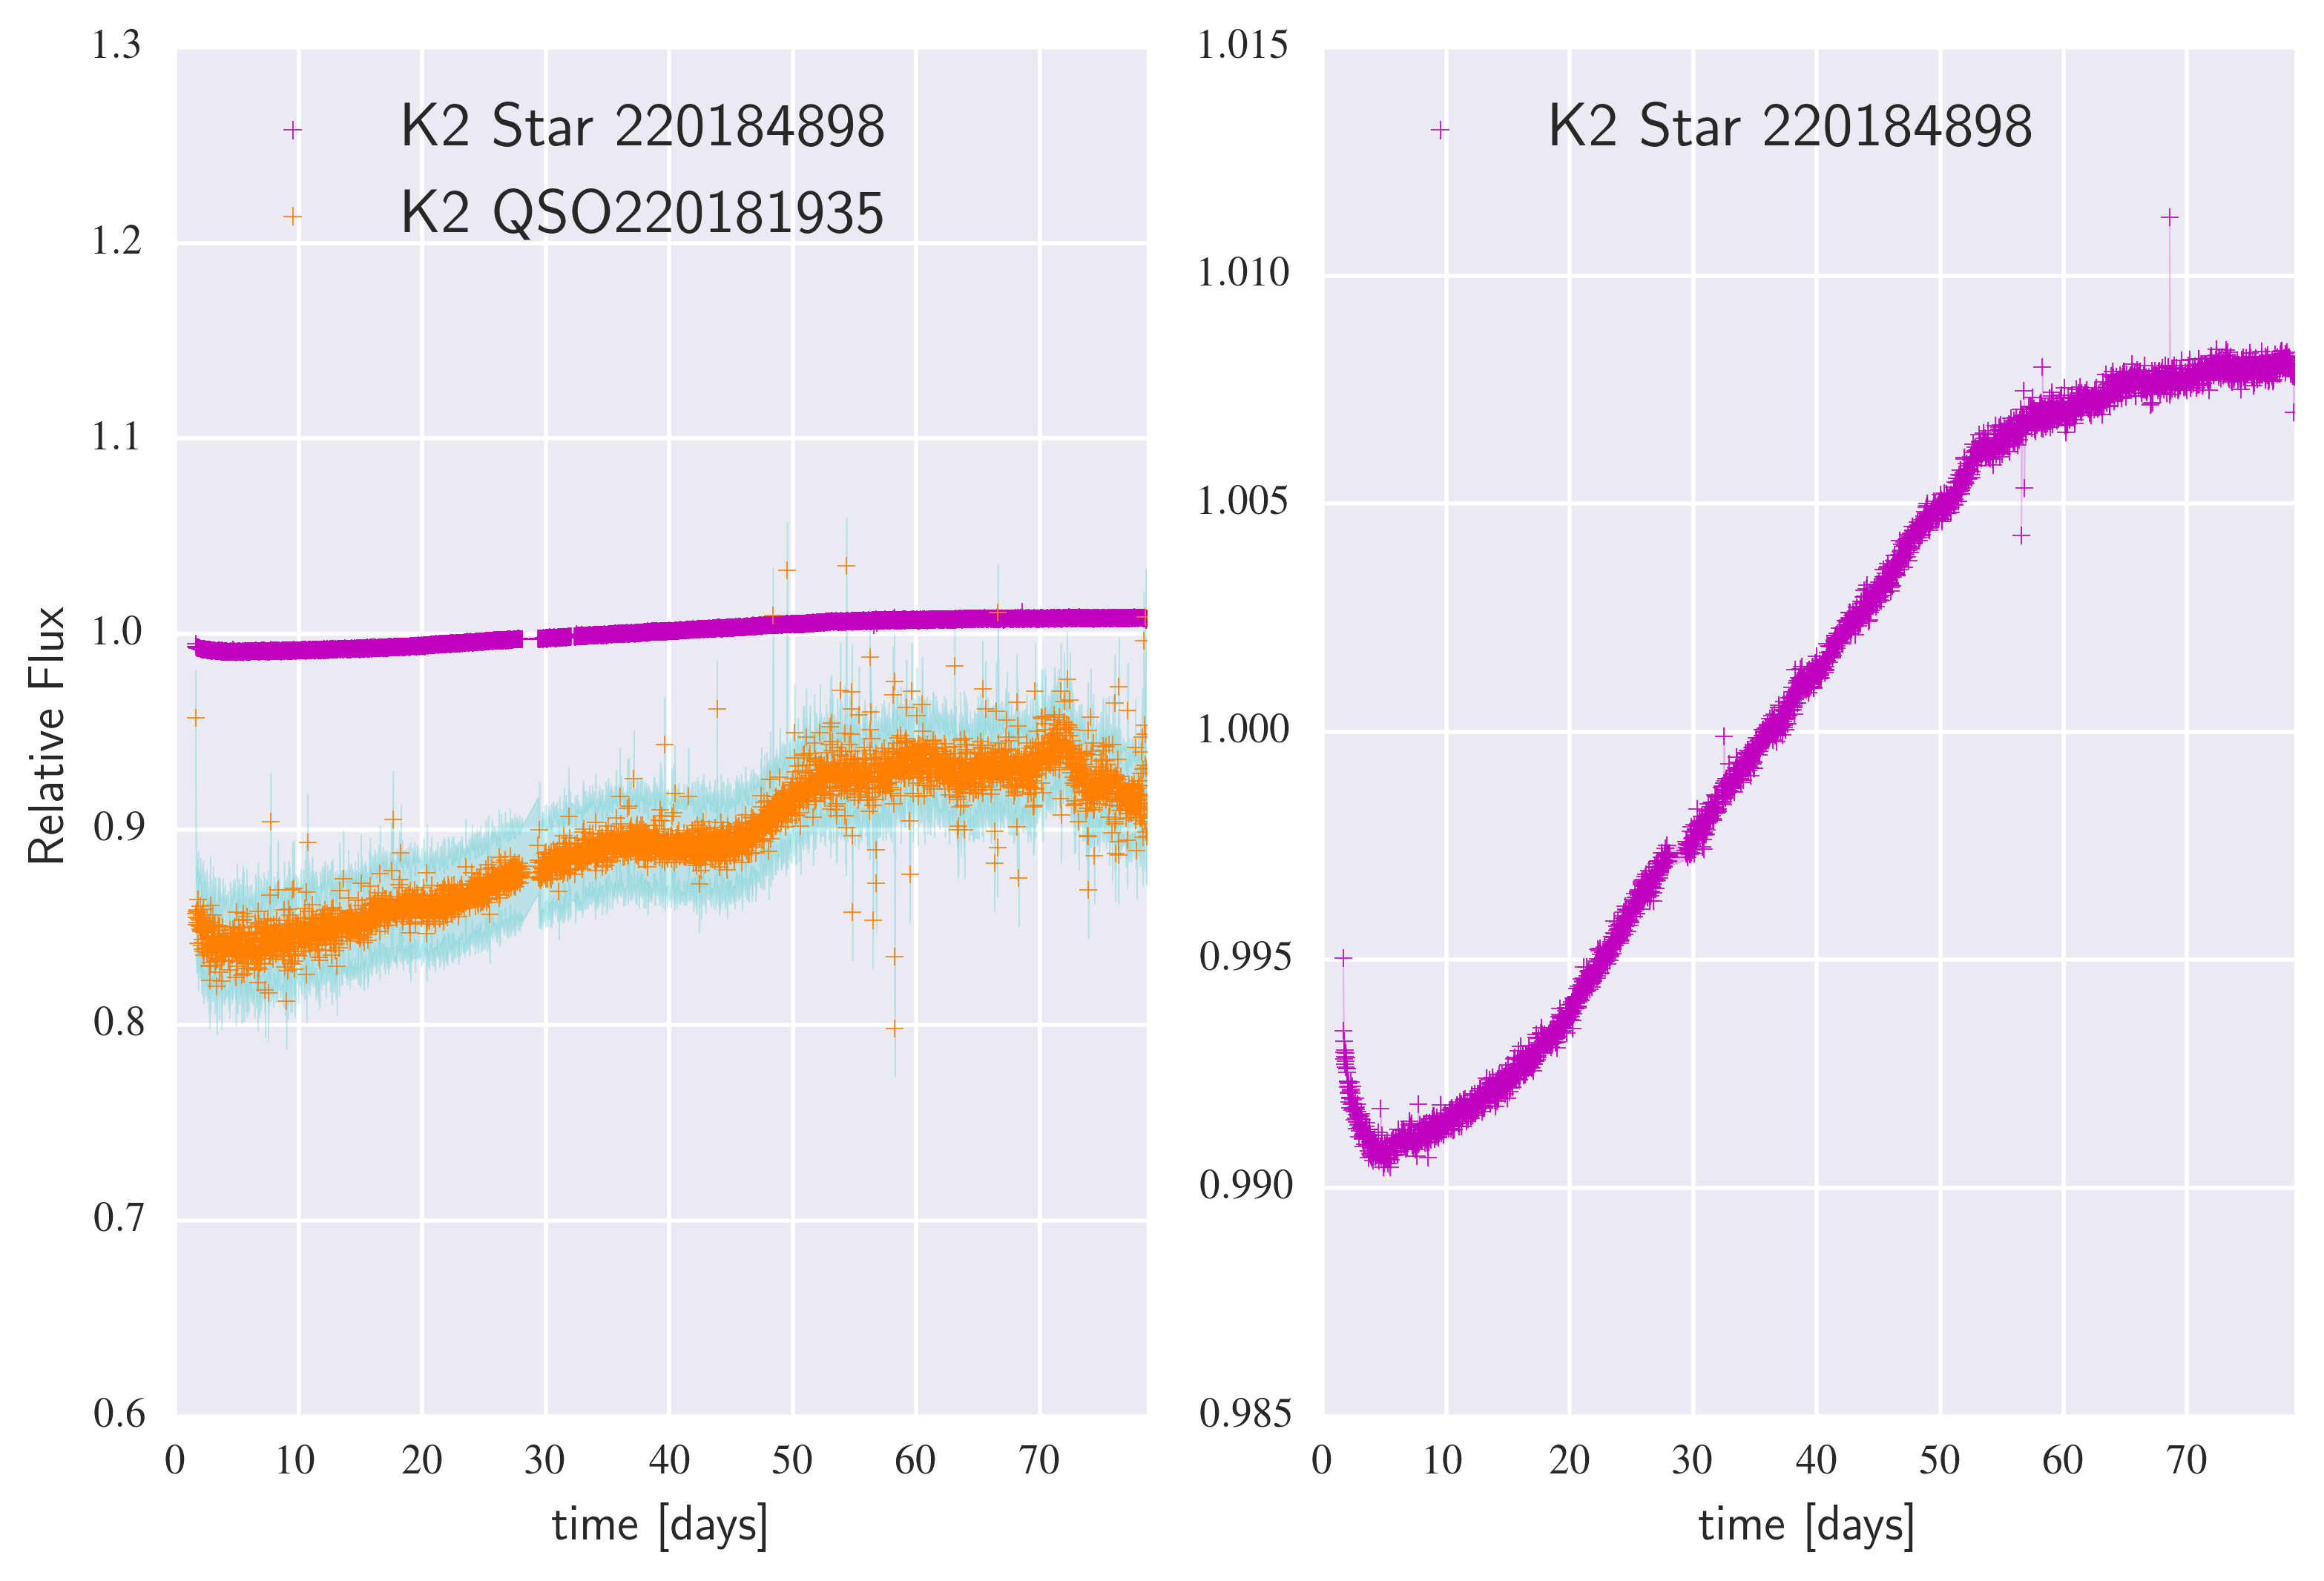
\includegraphics[width=\columnwidth]{220181935NearestNeighbor.png}
 	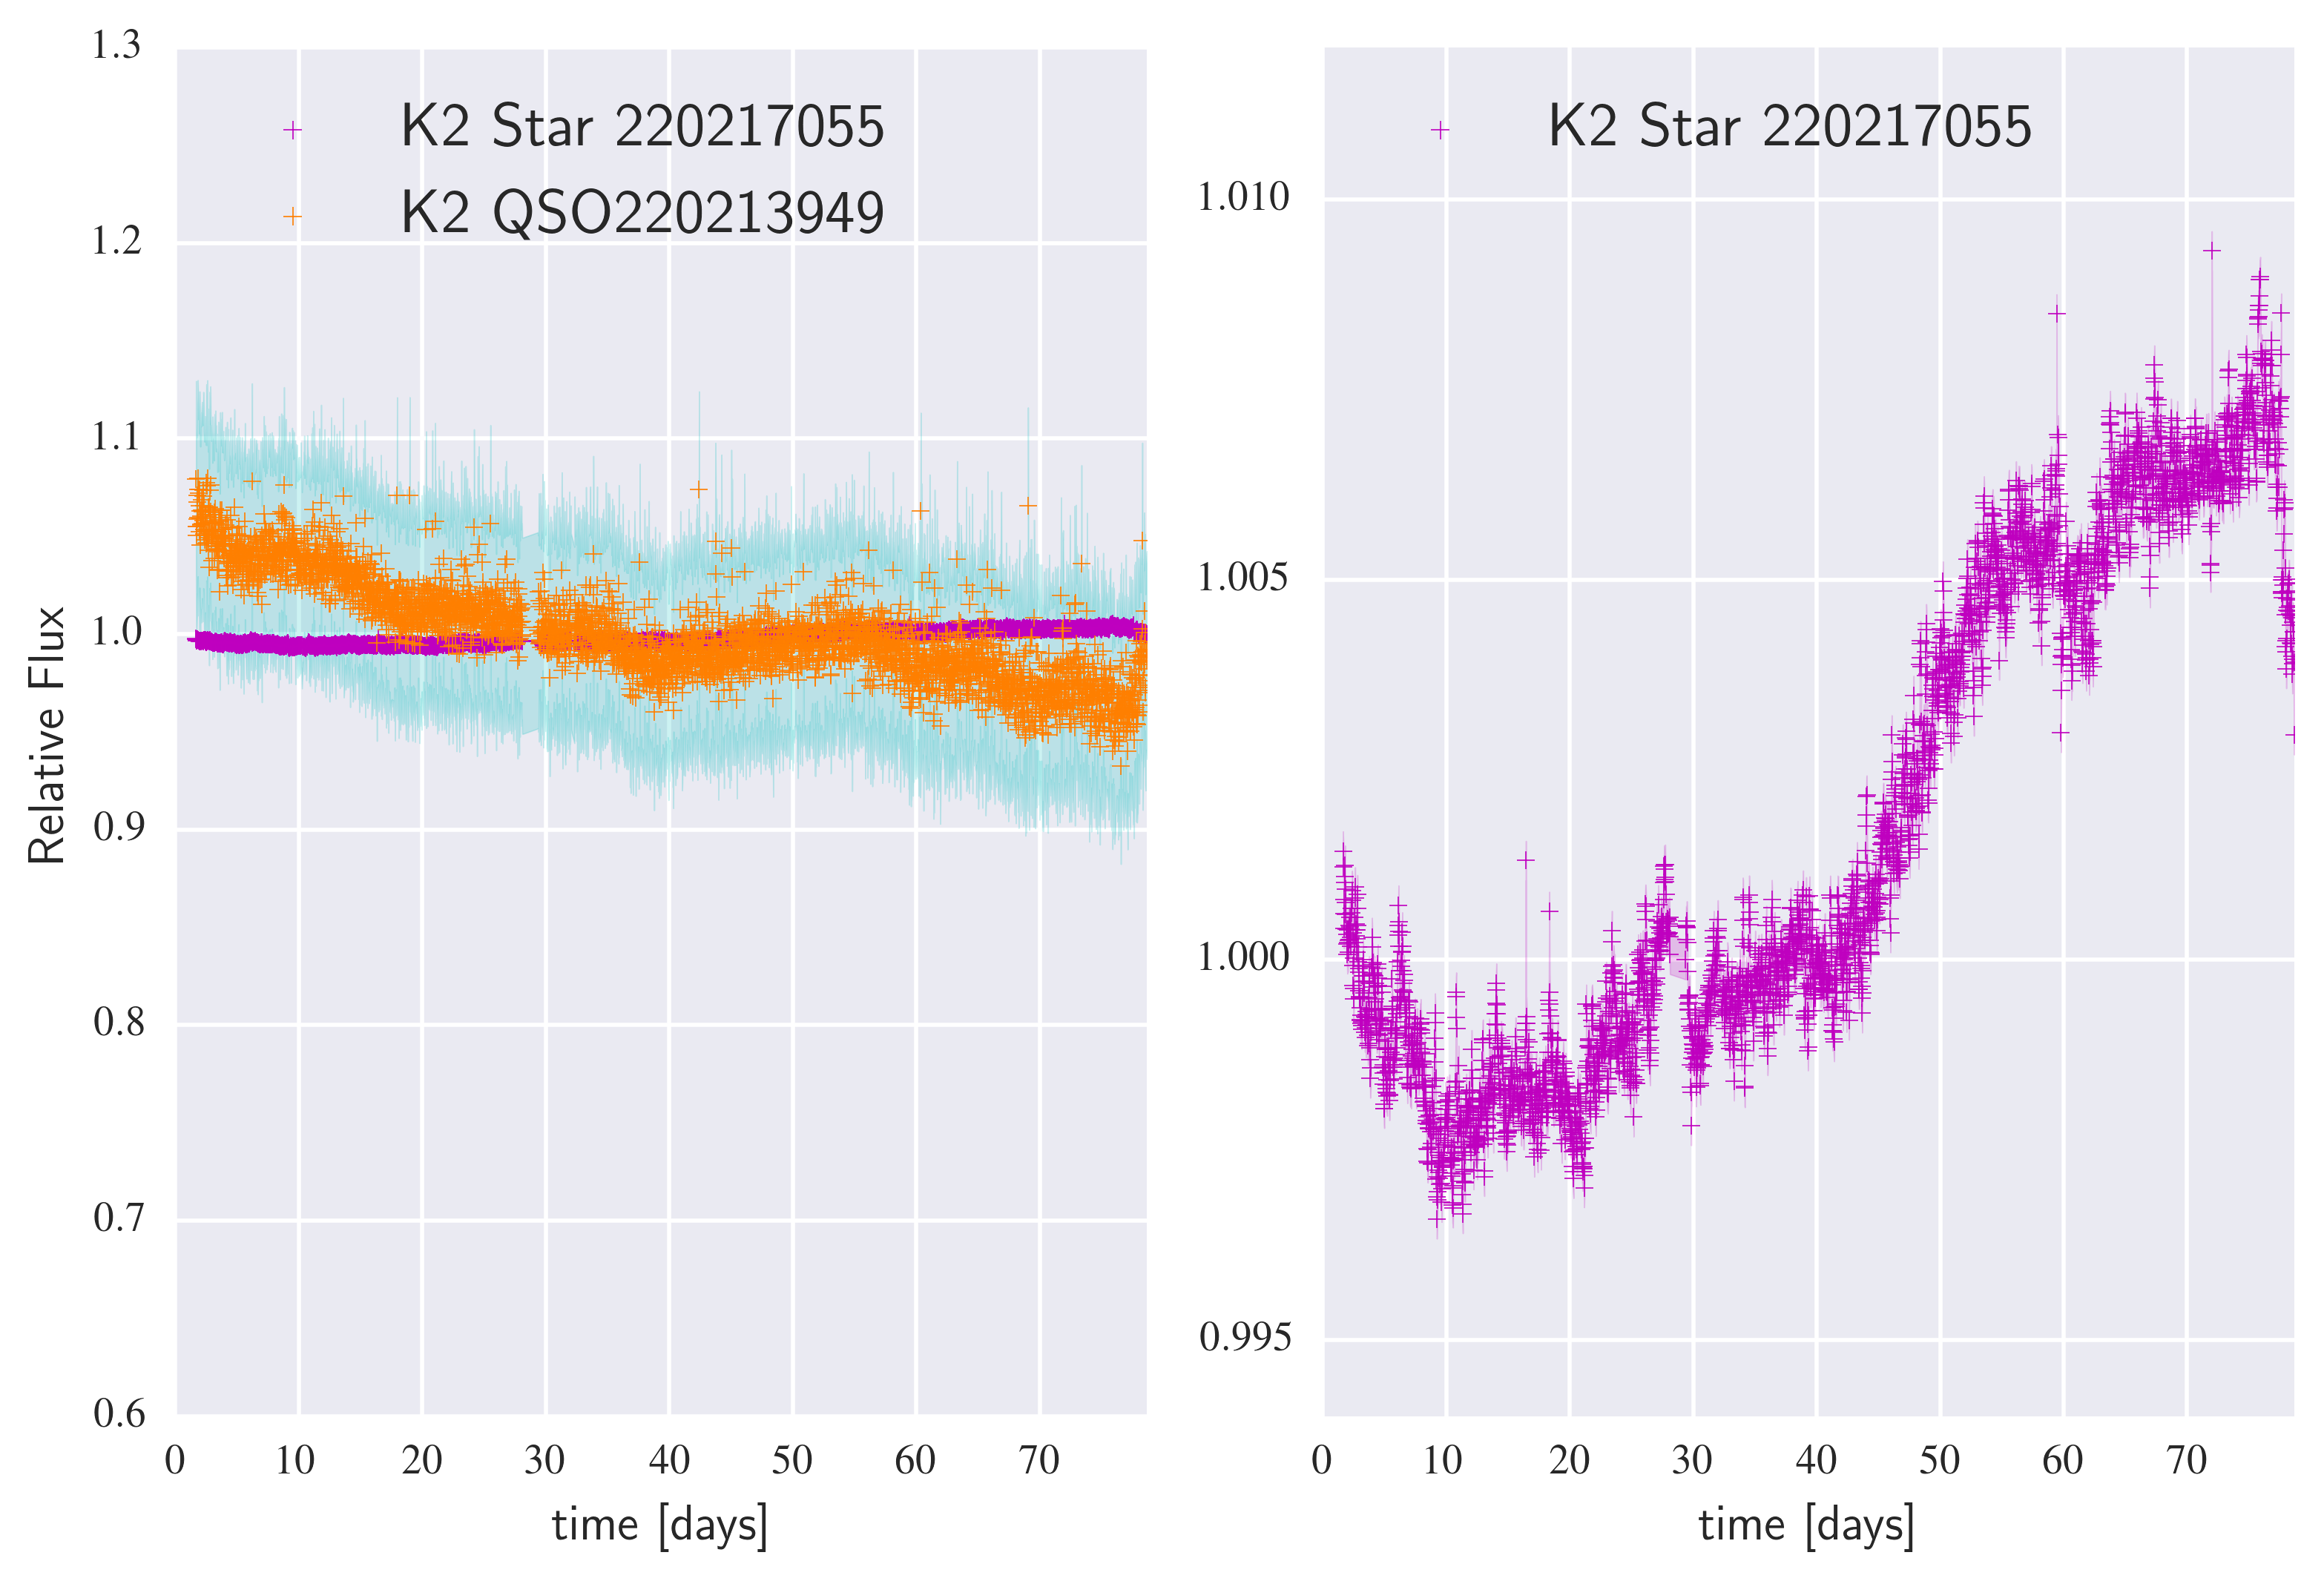
\includegraphics[width=\columnwidth]{220213949NearestNeighbor.png}
 	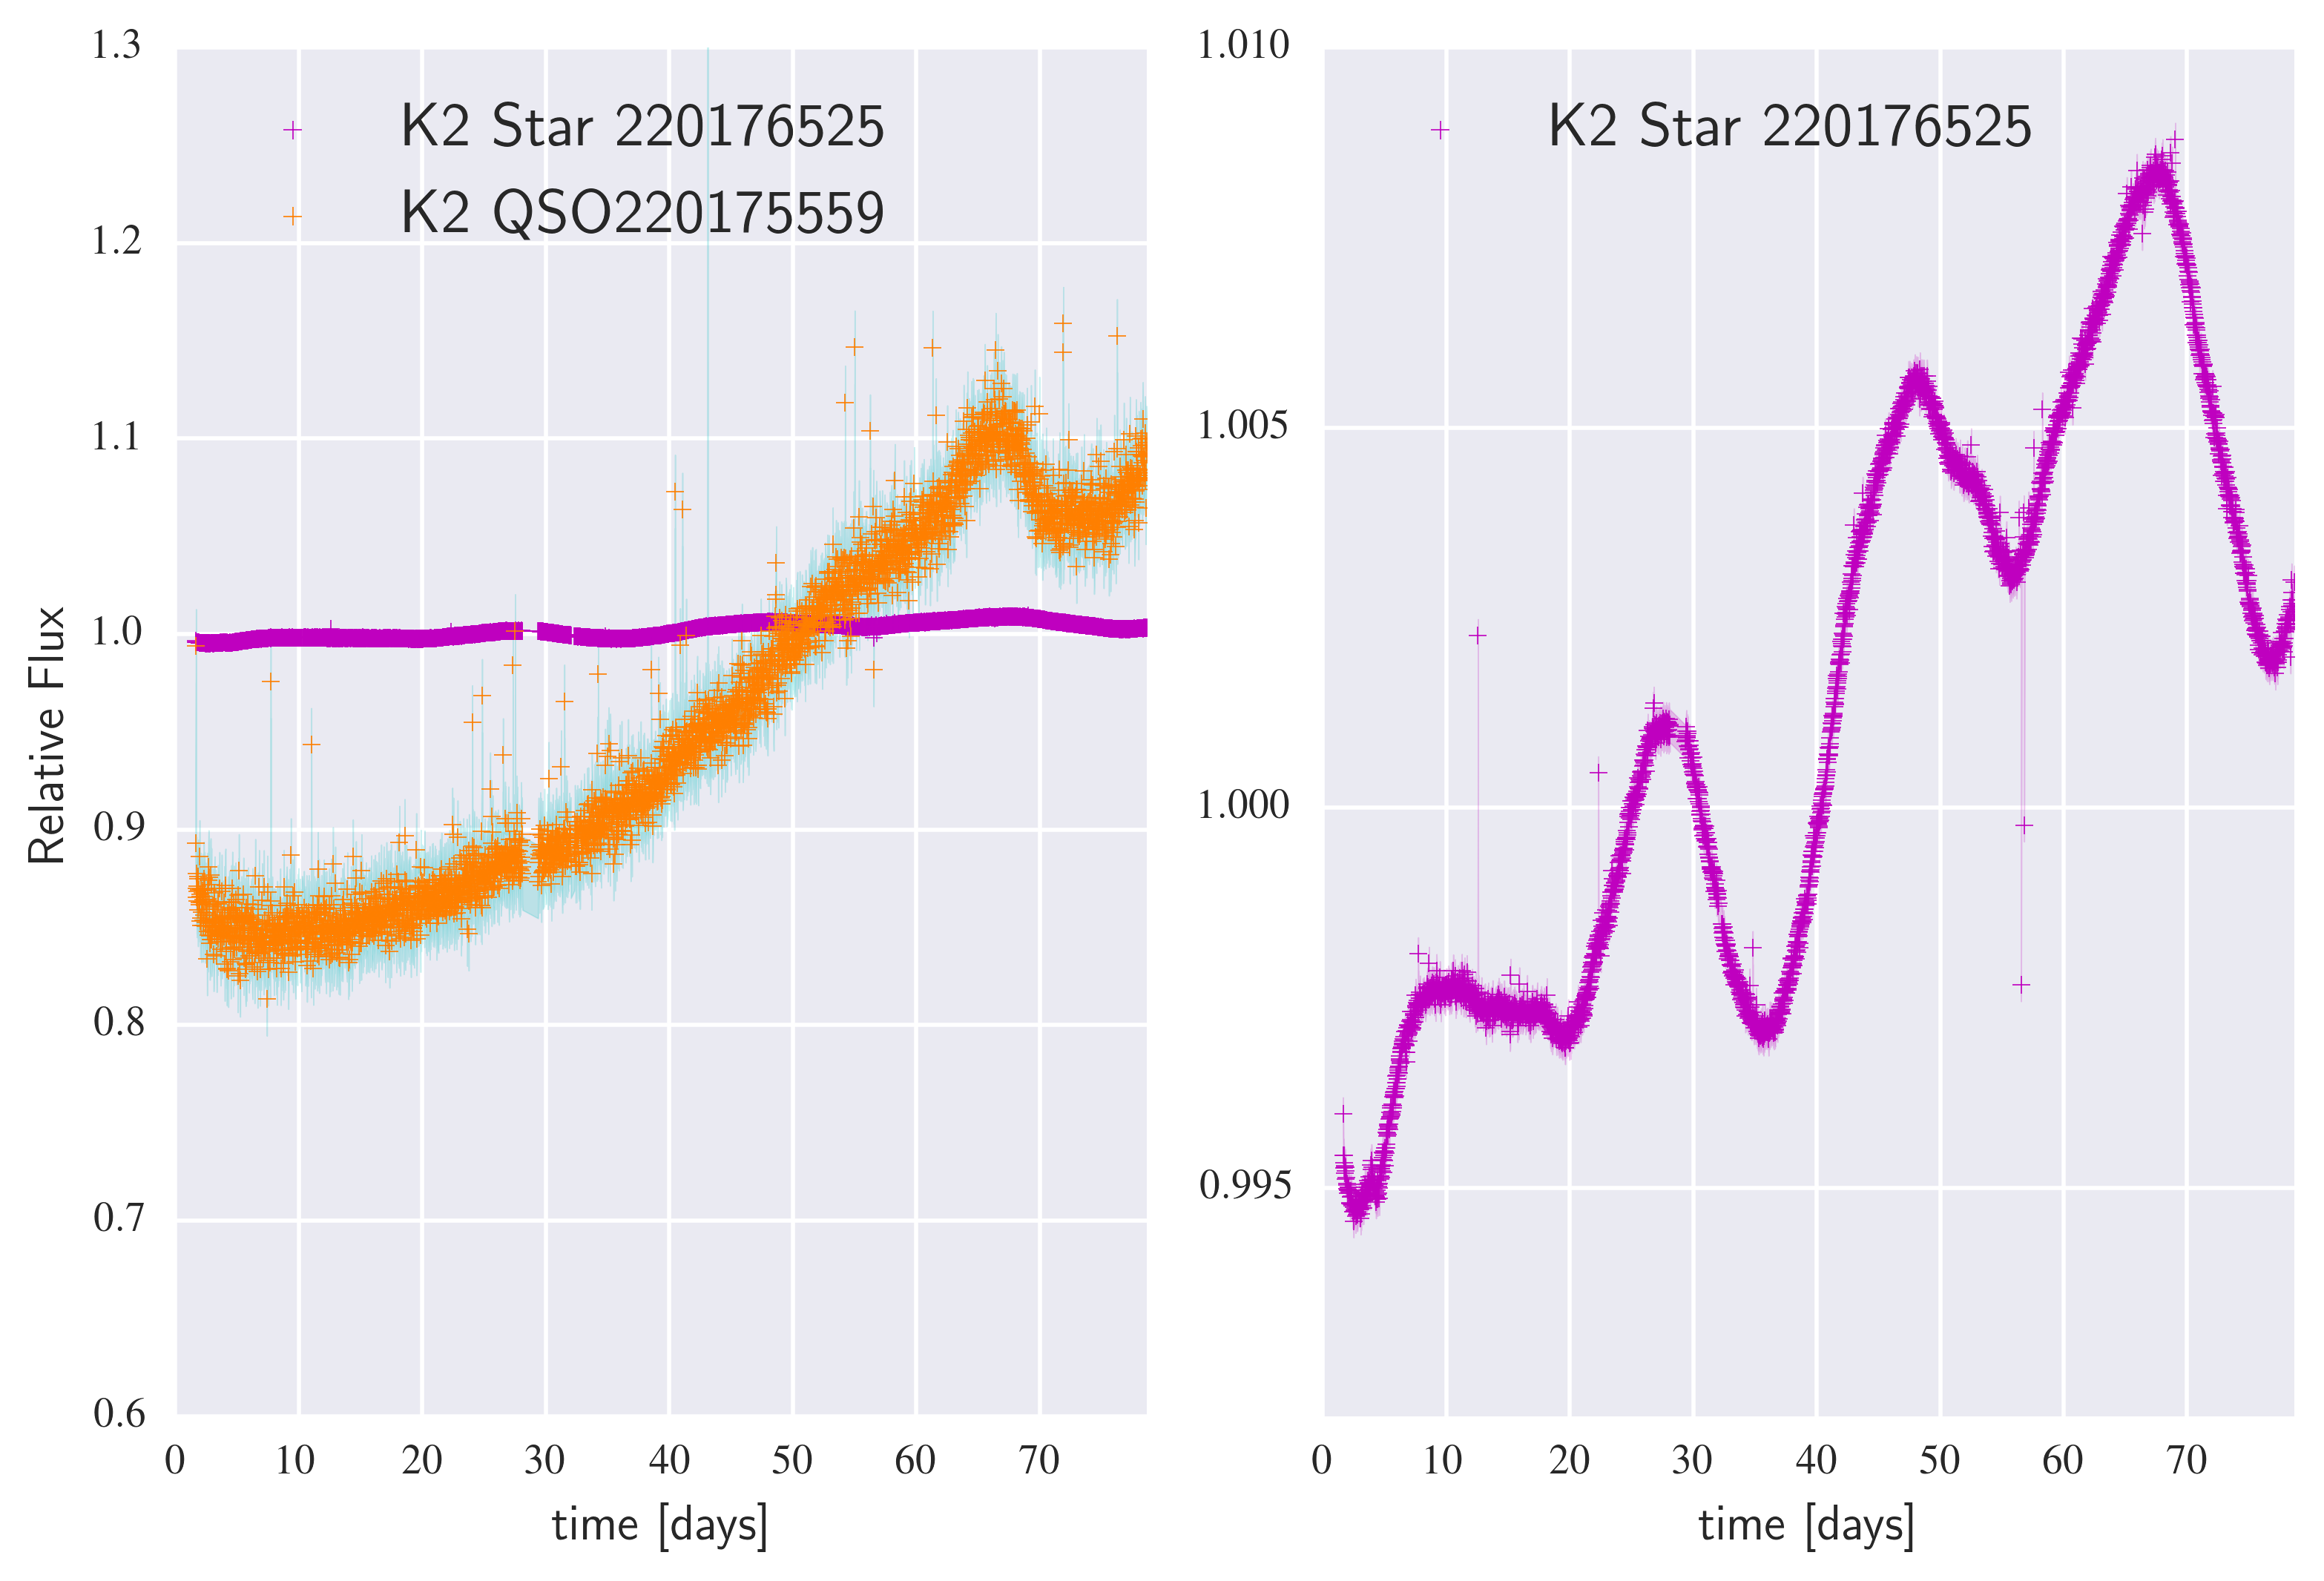
\includegraphics[width=\columnwidth]{220175559NearestNeighbor.png}
        	\caption{}
        	\label{fig:example_figure}
        \end{figure}      
        
        \begin{figure}
        	% To include a figure from a file named example.*
        	% Allowable file formats are eps or ps if compiling using latex
        	% or pdf, png, jpg if compiling using pdflatex
 	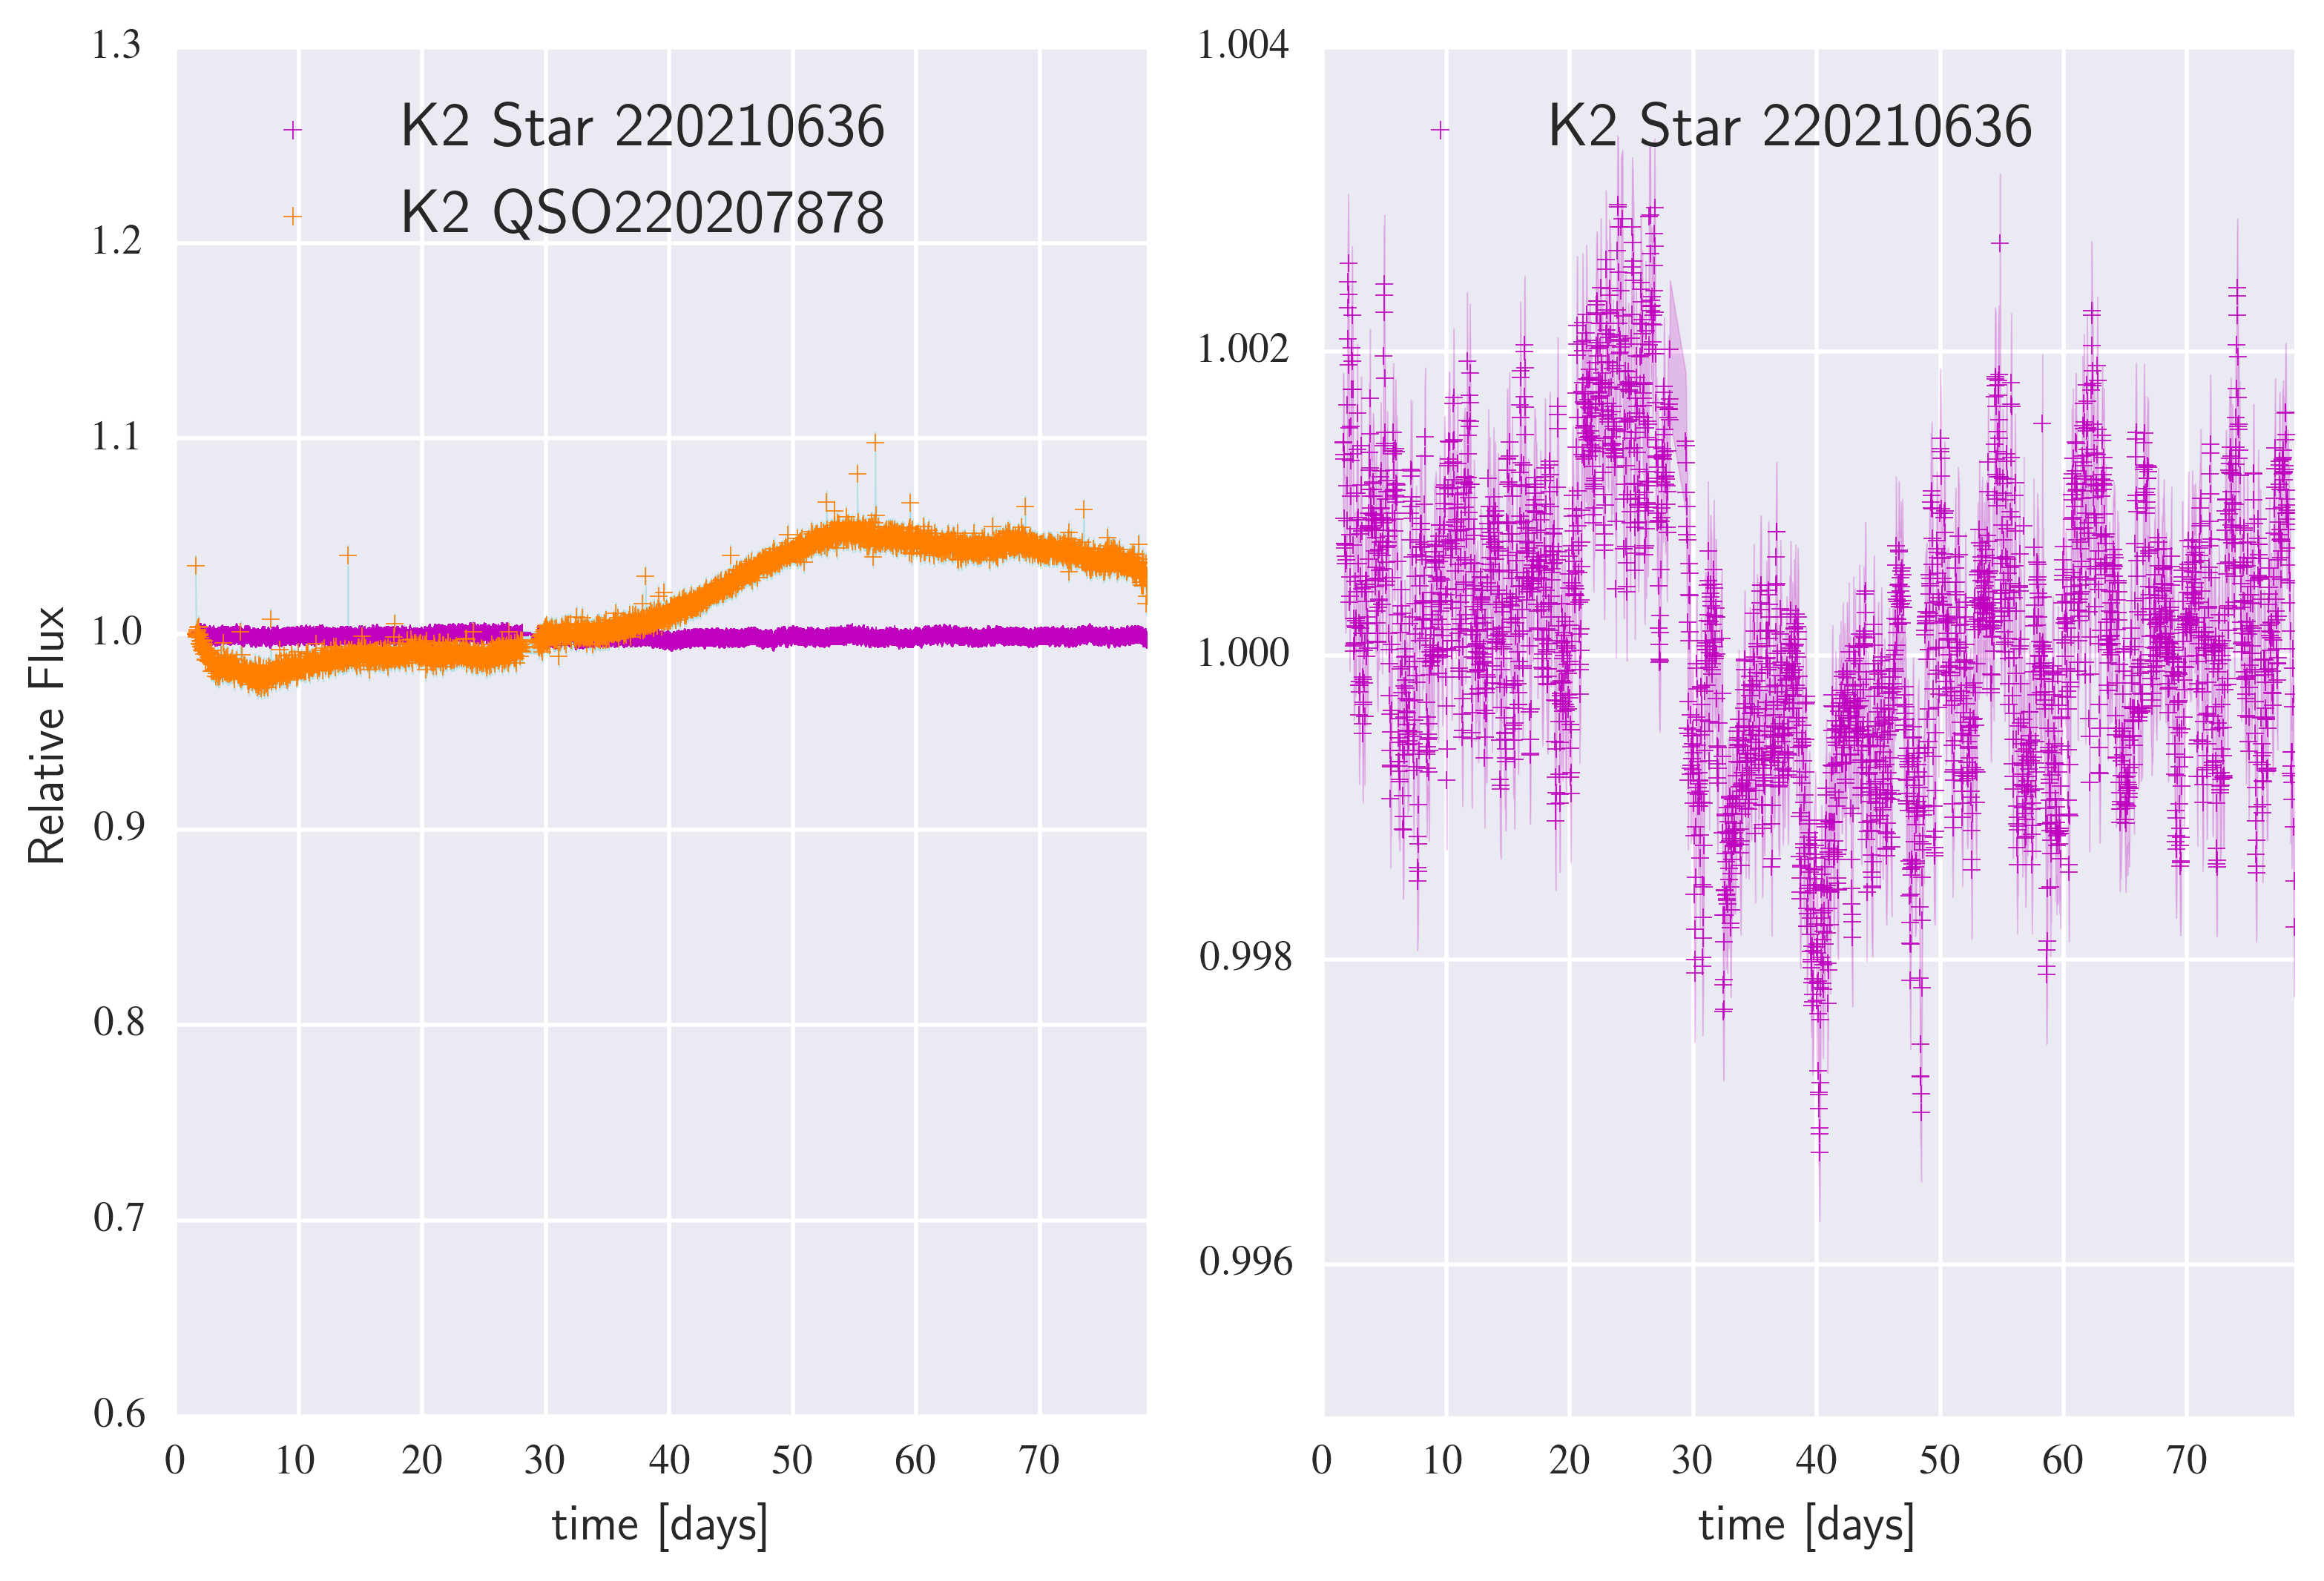
\includegraphics[width=\columnwidth]{220207878NearestNeighbor.png}
 	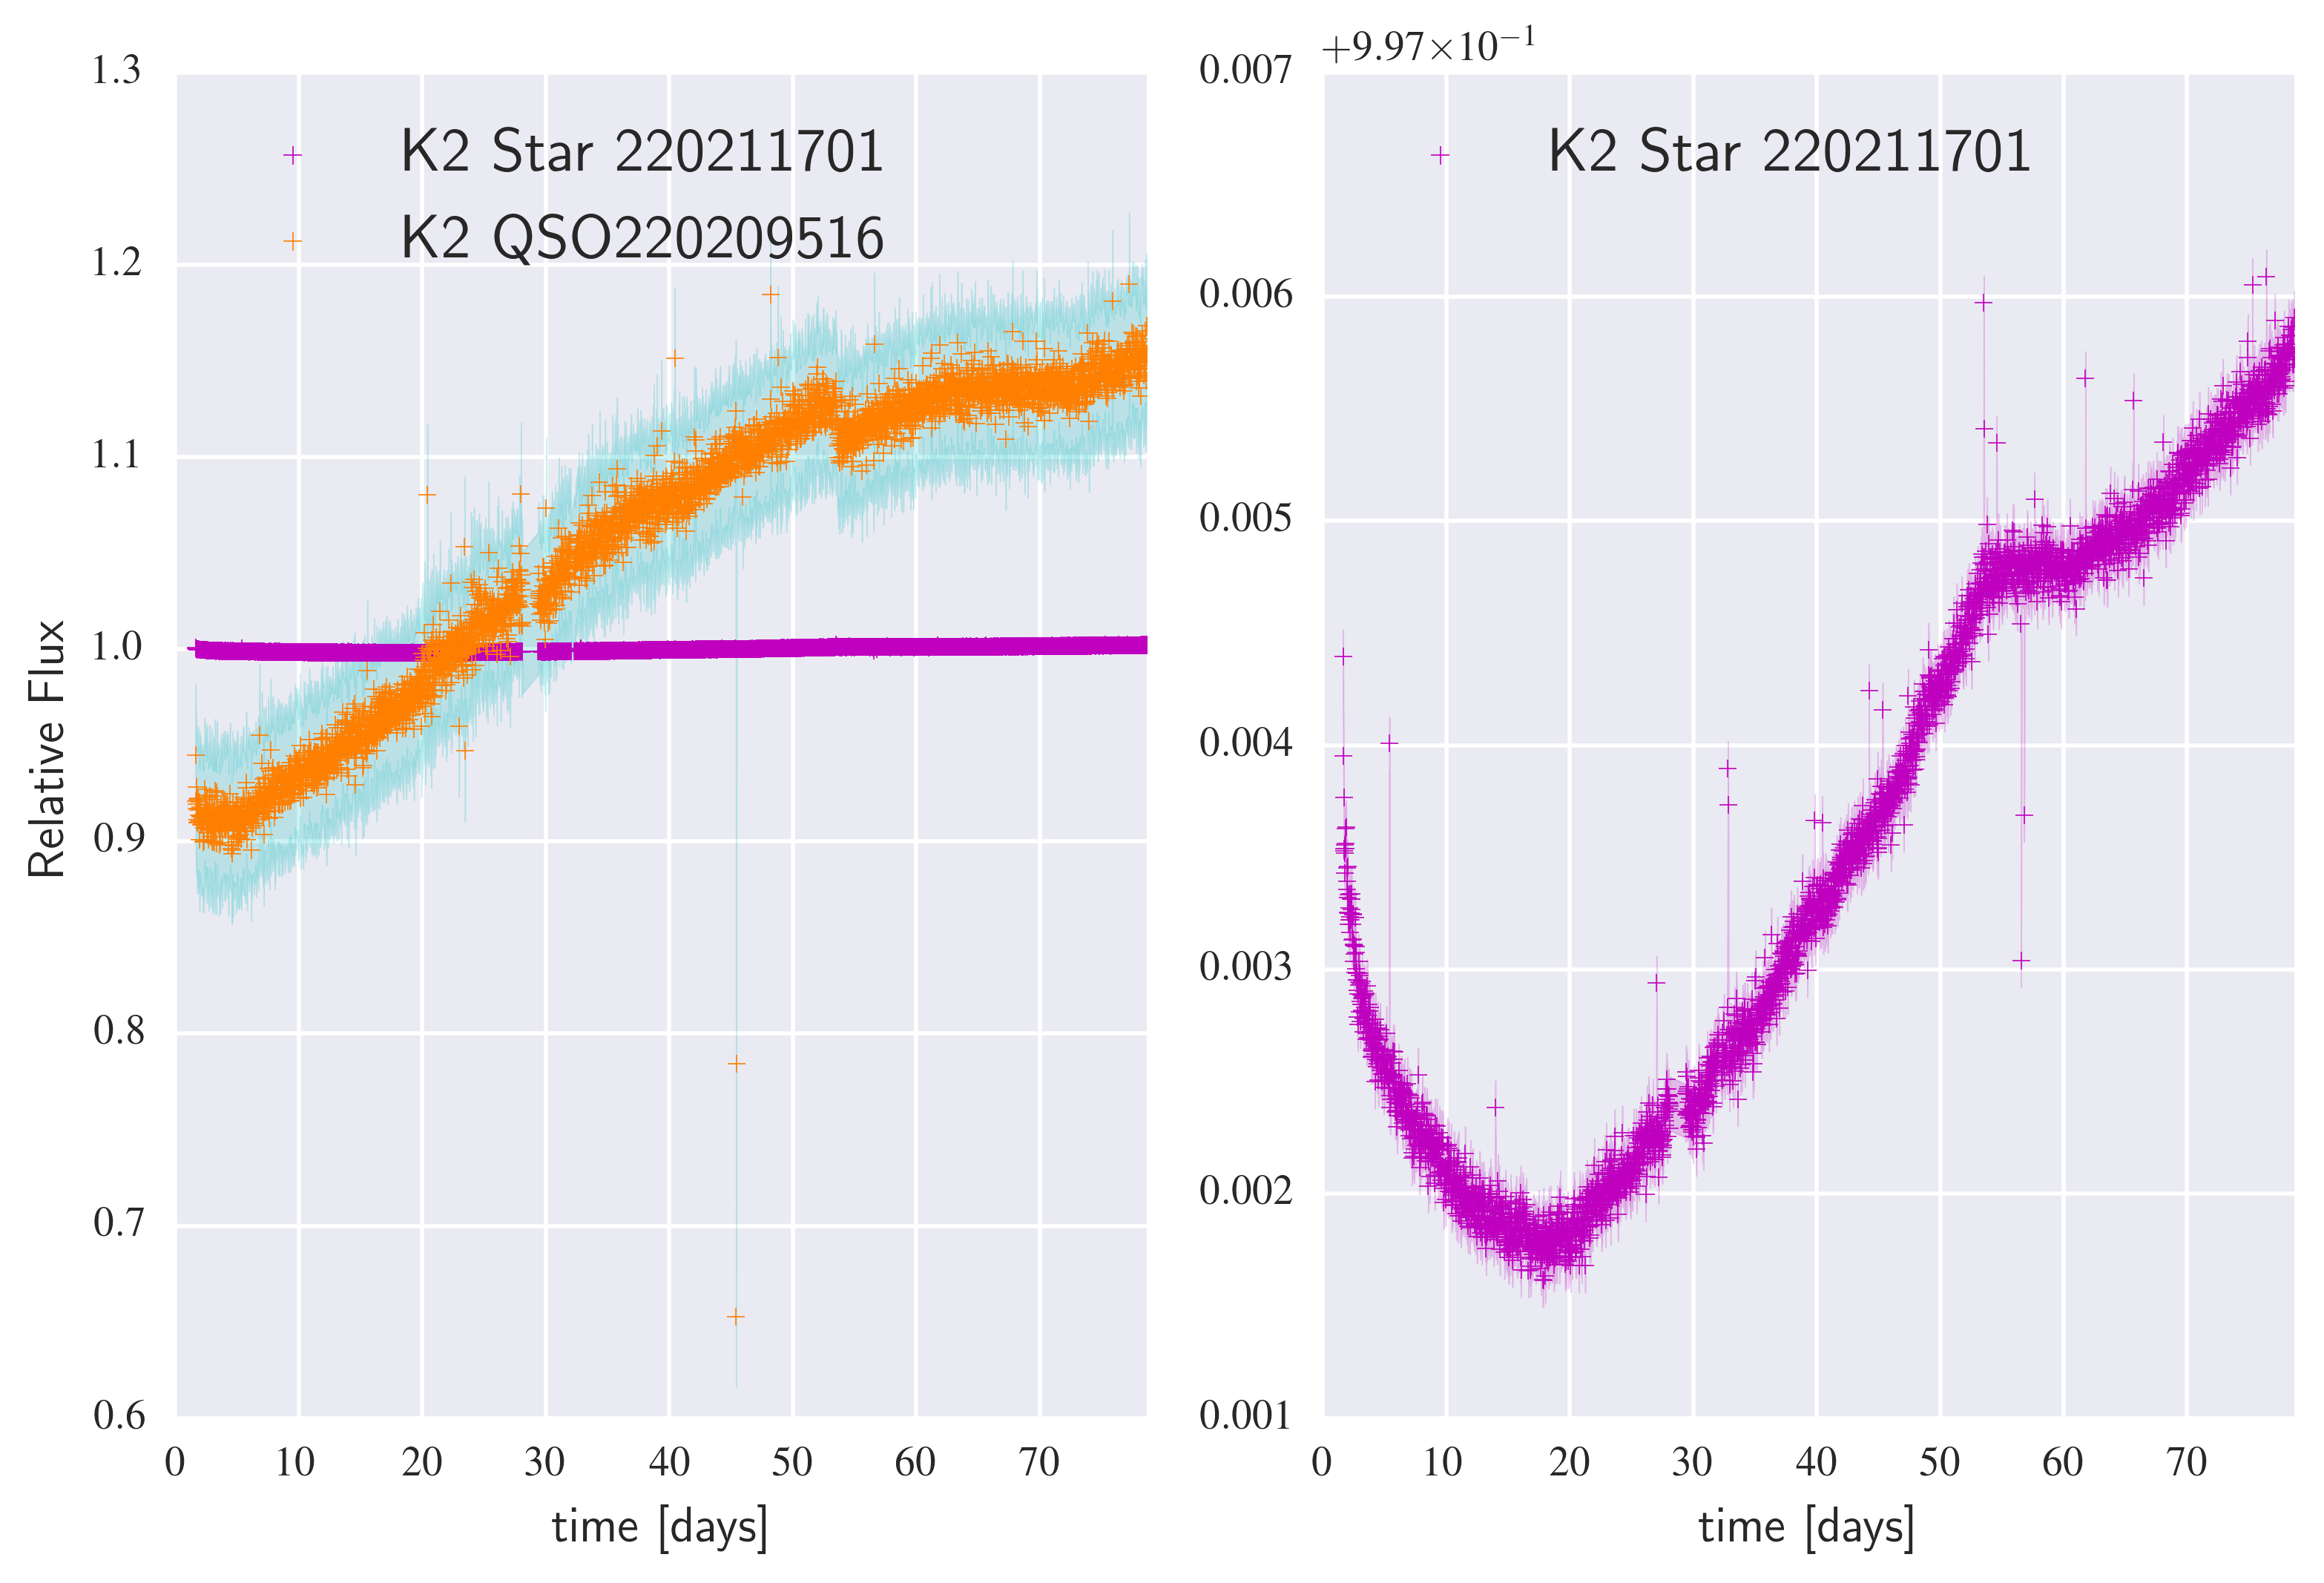
\includegraphics[width=\columnwidth]{220209516NearestNeighbor.png}
 	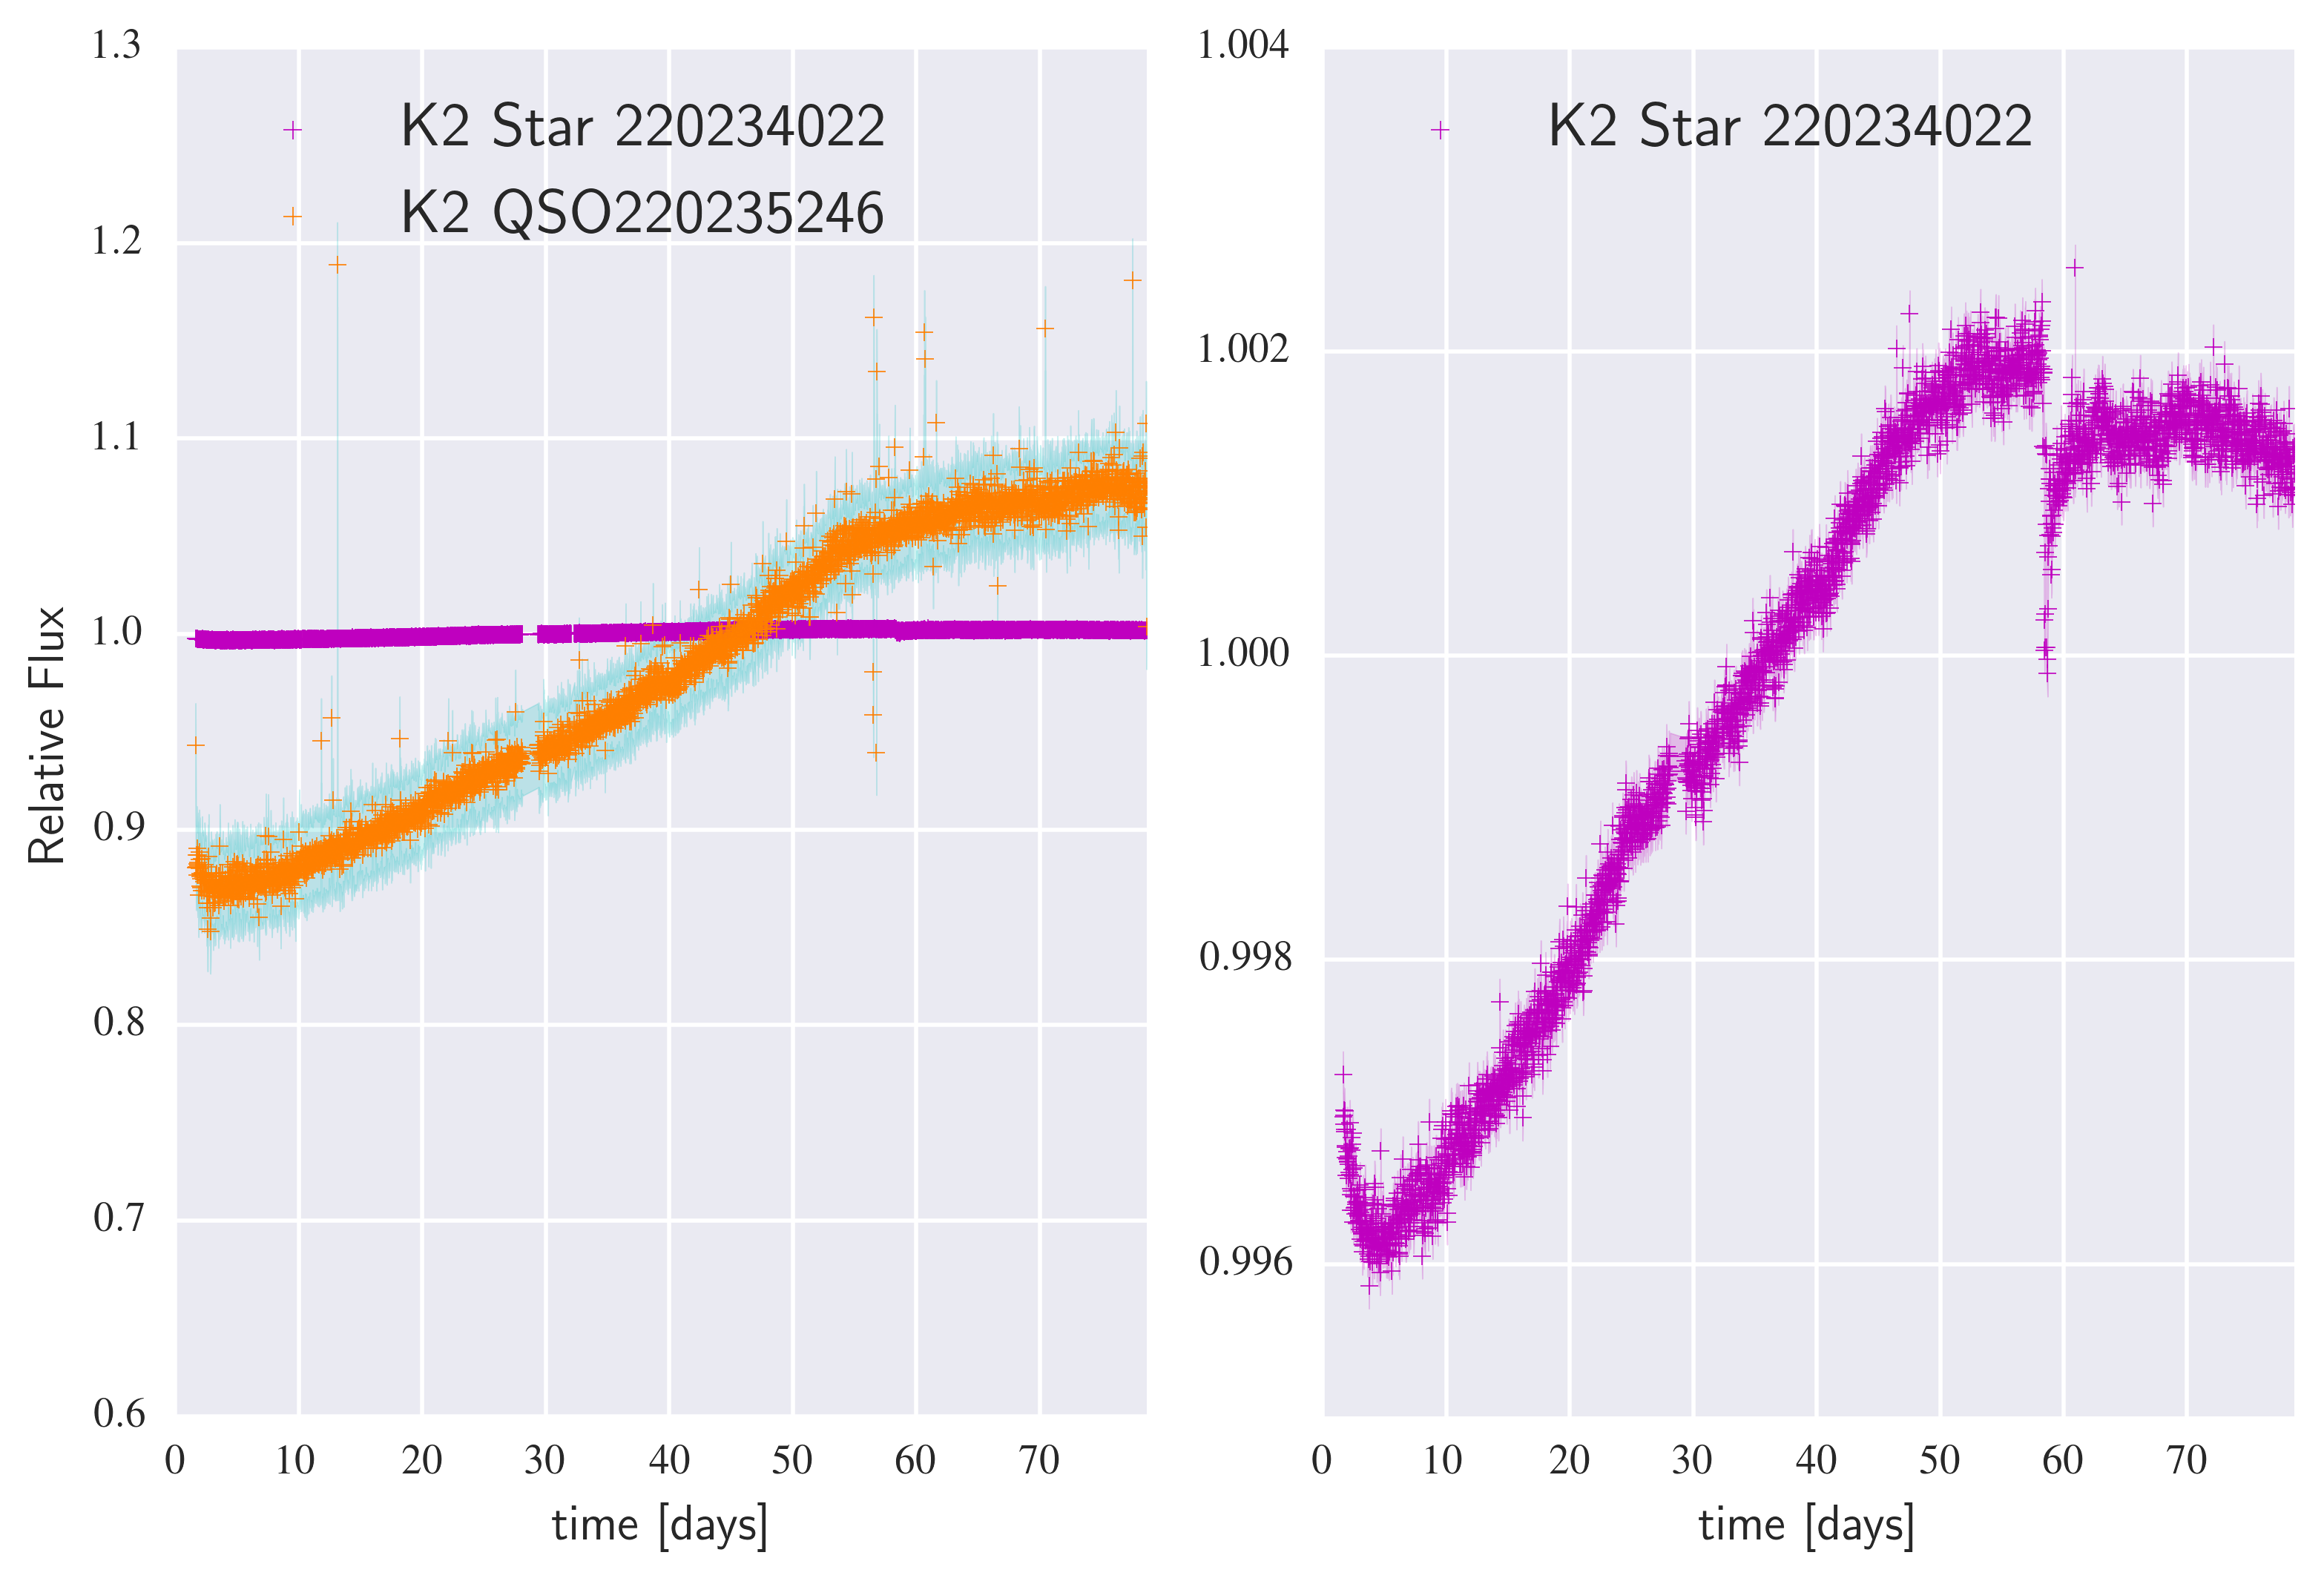
\includegraphics[width=\columnwidth]{220235246NearestNeighbor.png}
        	\caption{}
        	\label{fig:example_figure}
        \end{figure}      
        
        
        \begin{figure}
        	% To include a figure from a file named example.*
        	% Allowable file formats are eps or ps if compiling using latex
        	% or pdf, png, jpg if compiling using pdflatex
 	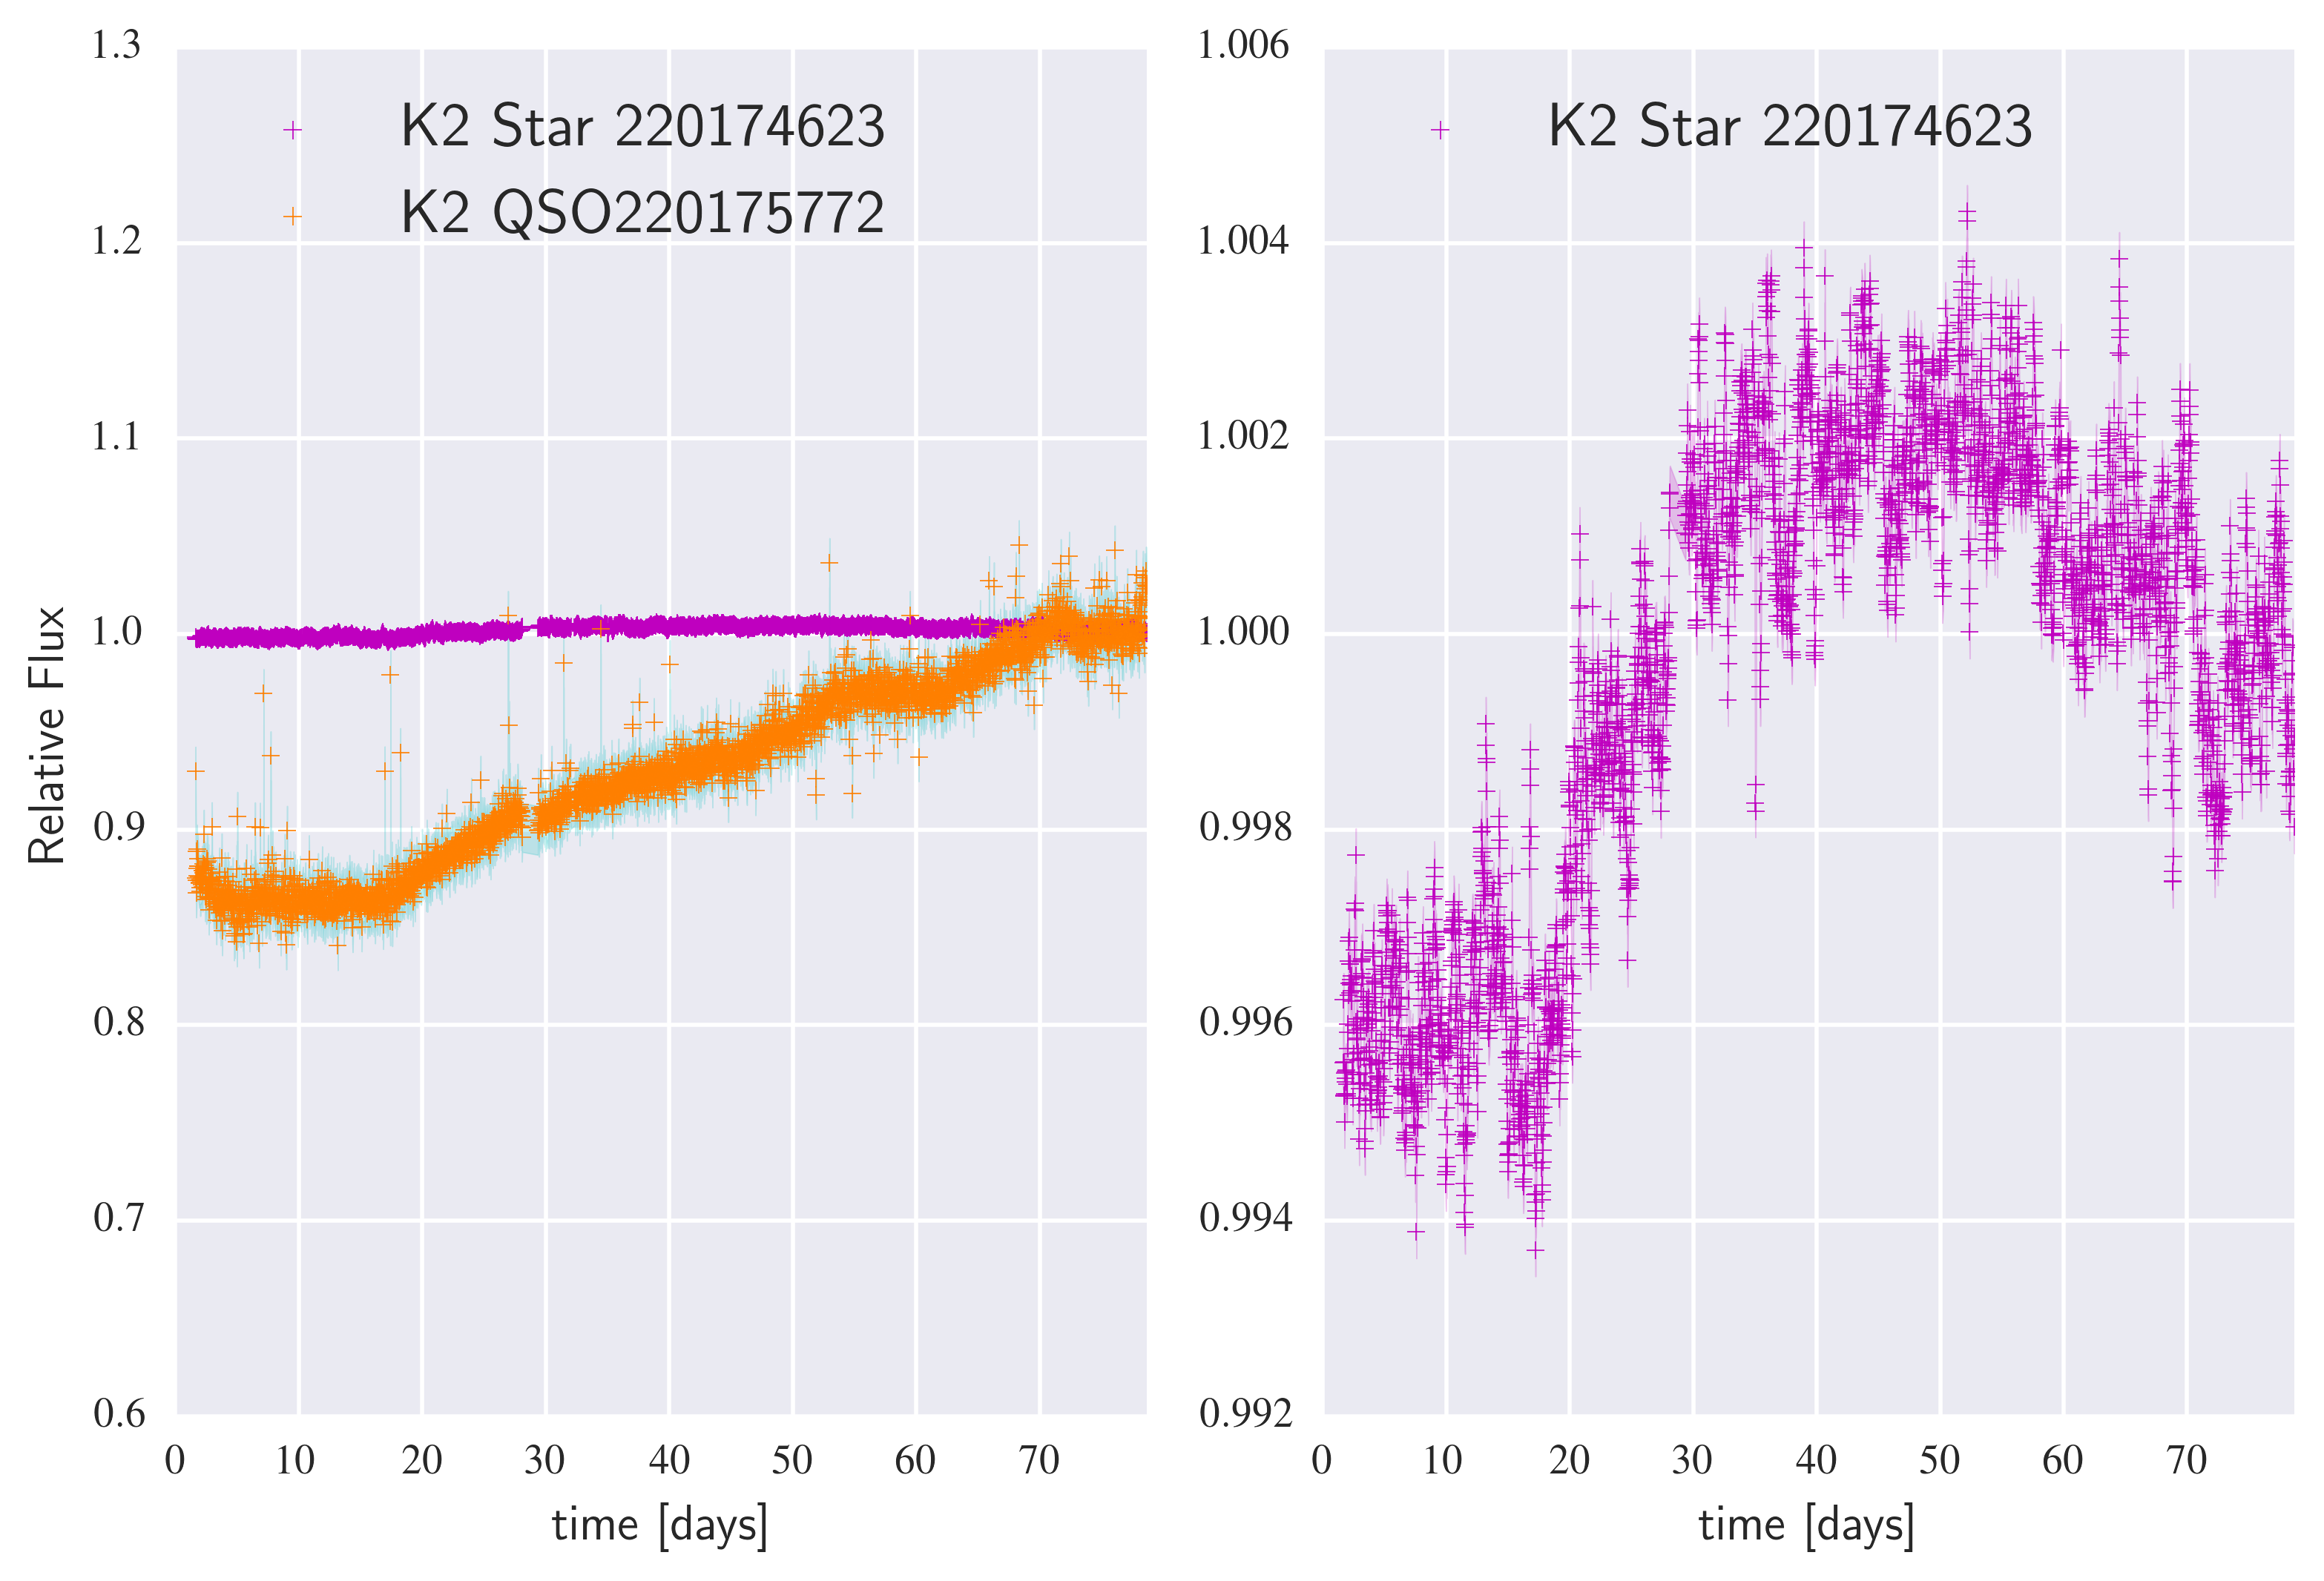
\includegraphics[width=\columnwidth]{220175772NearestNeighbor.png}
 	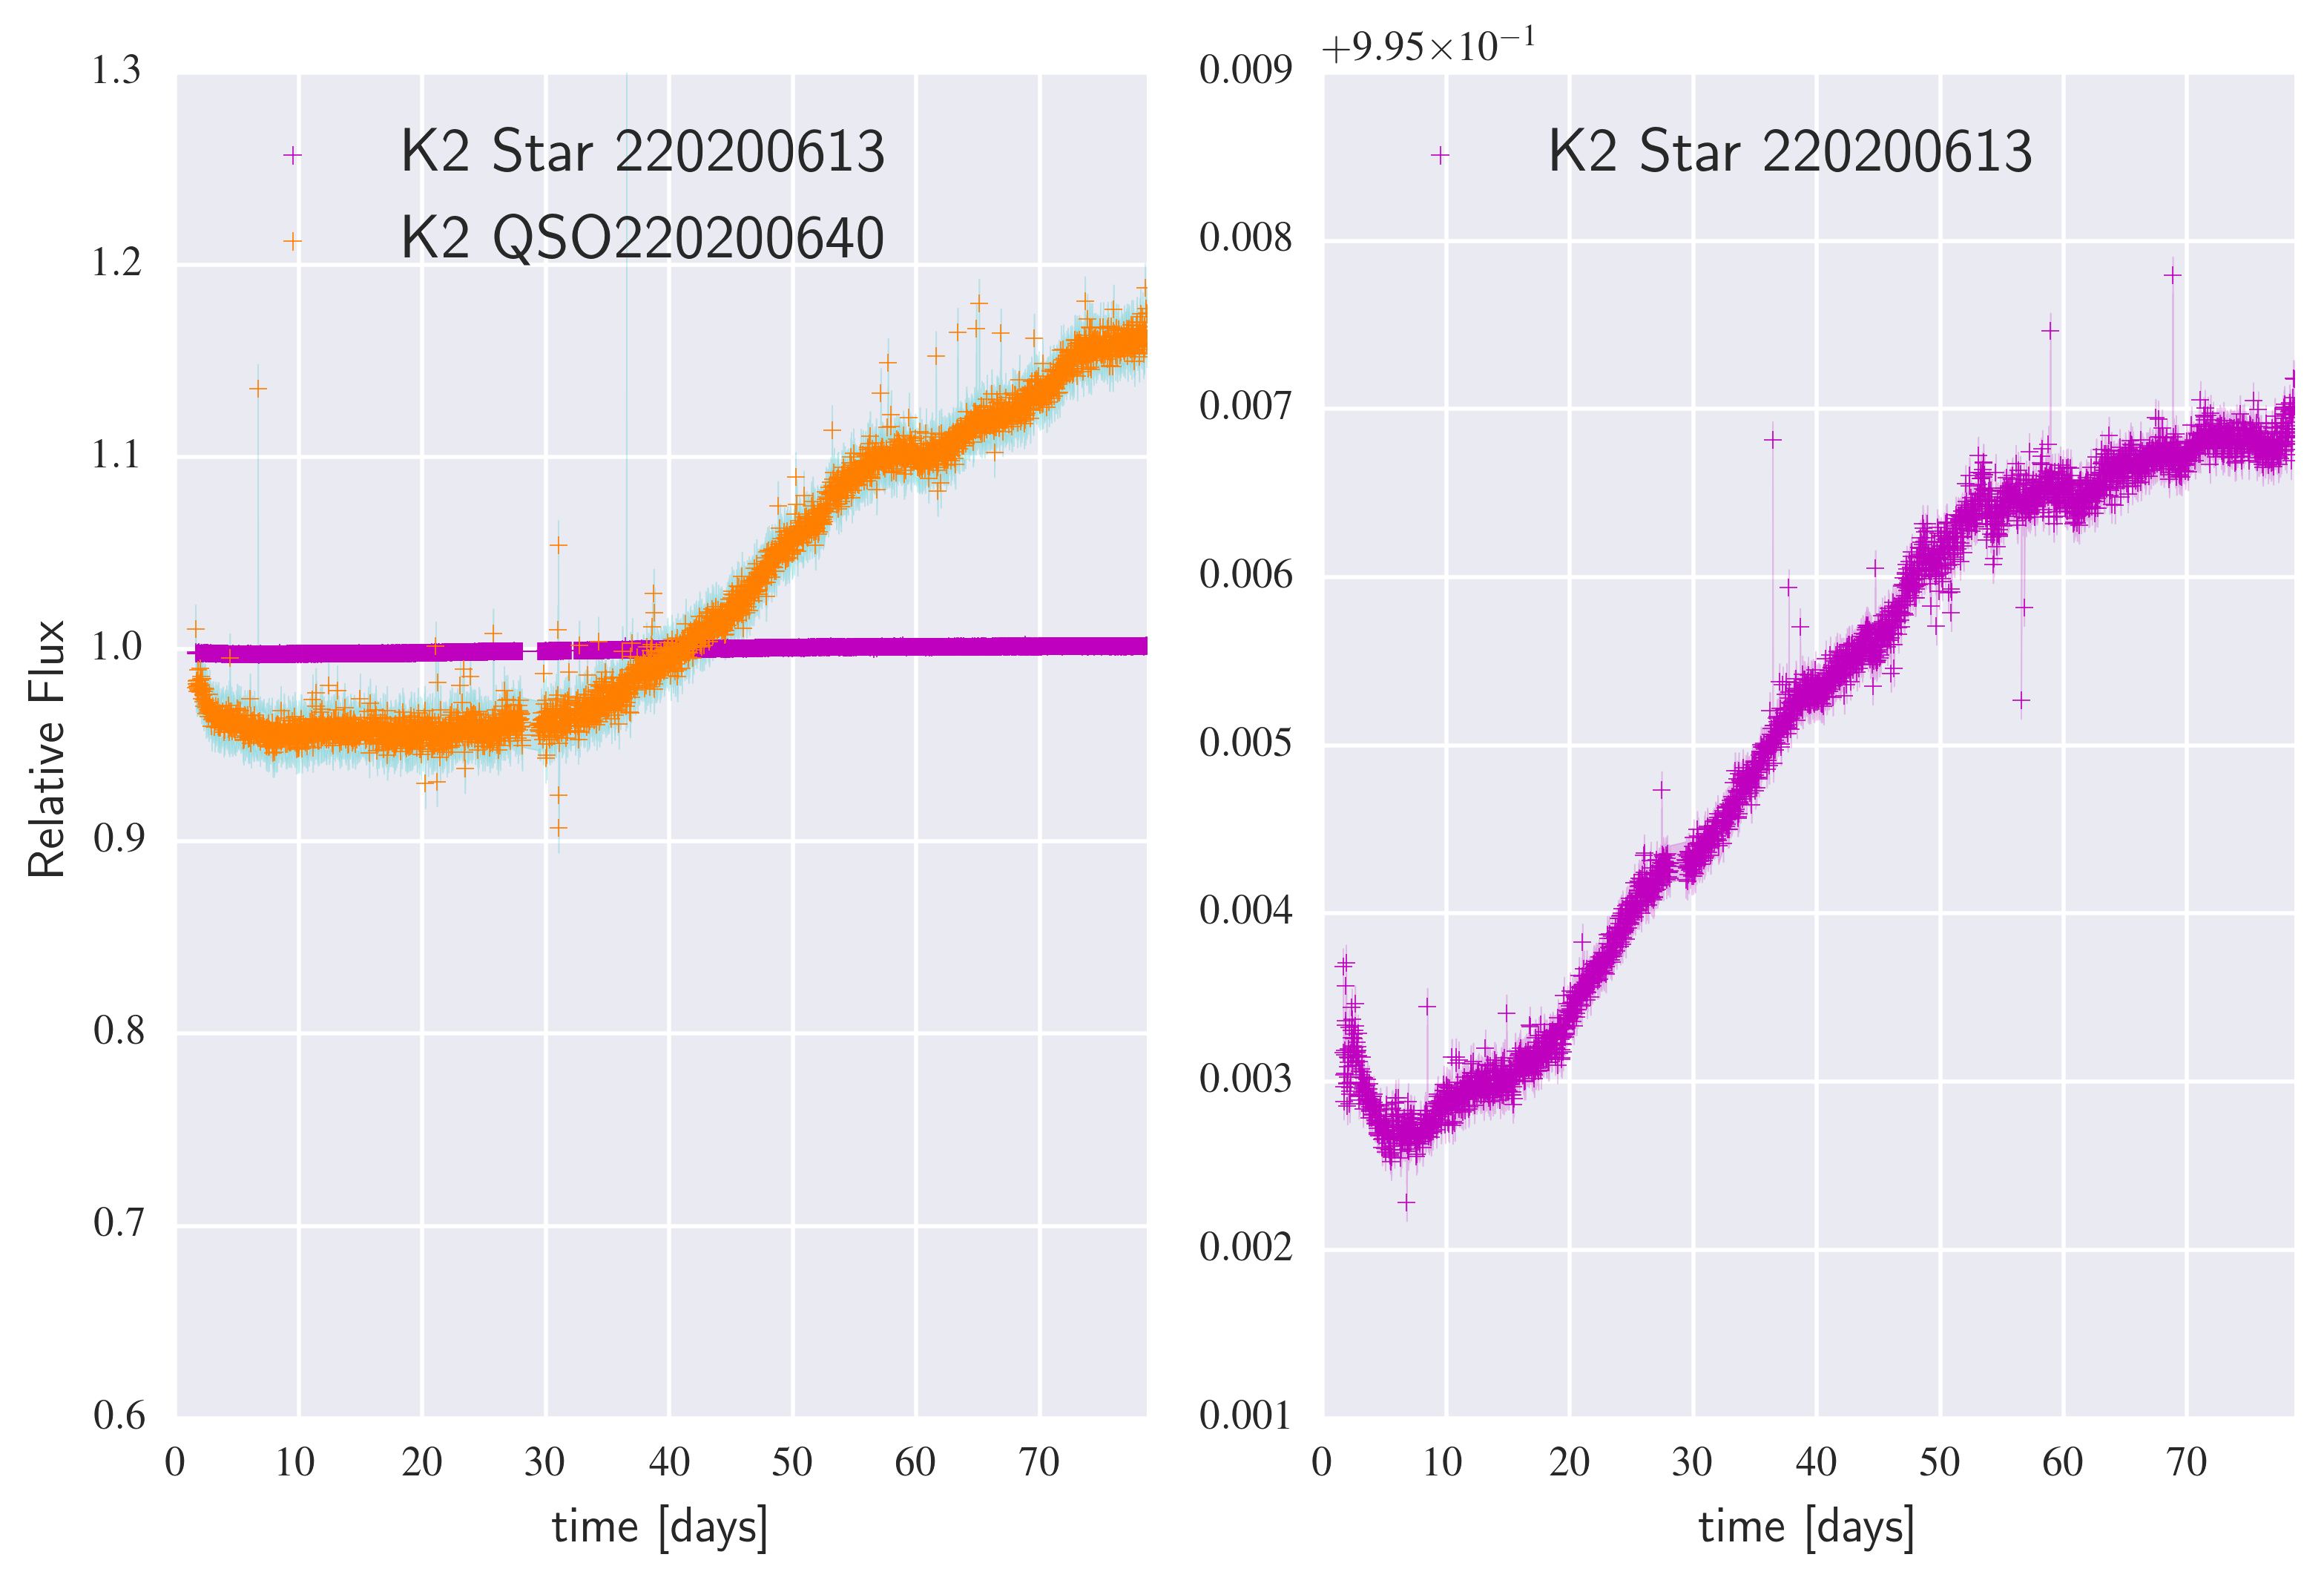
\includegraphics[width=\columnwidth]{220200640NearestNeighbor.png}
 	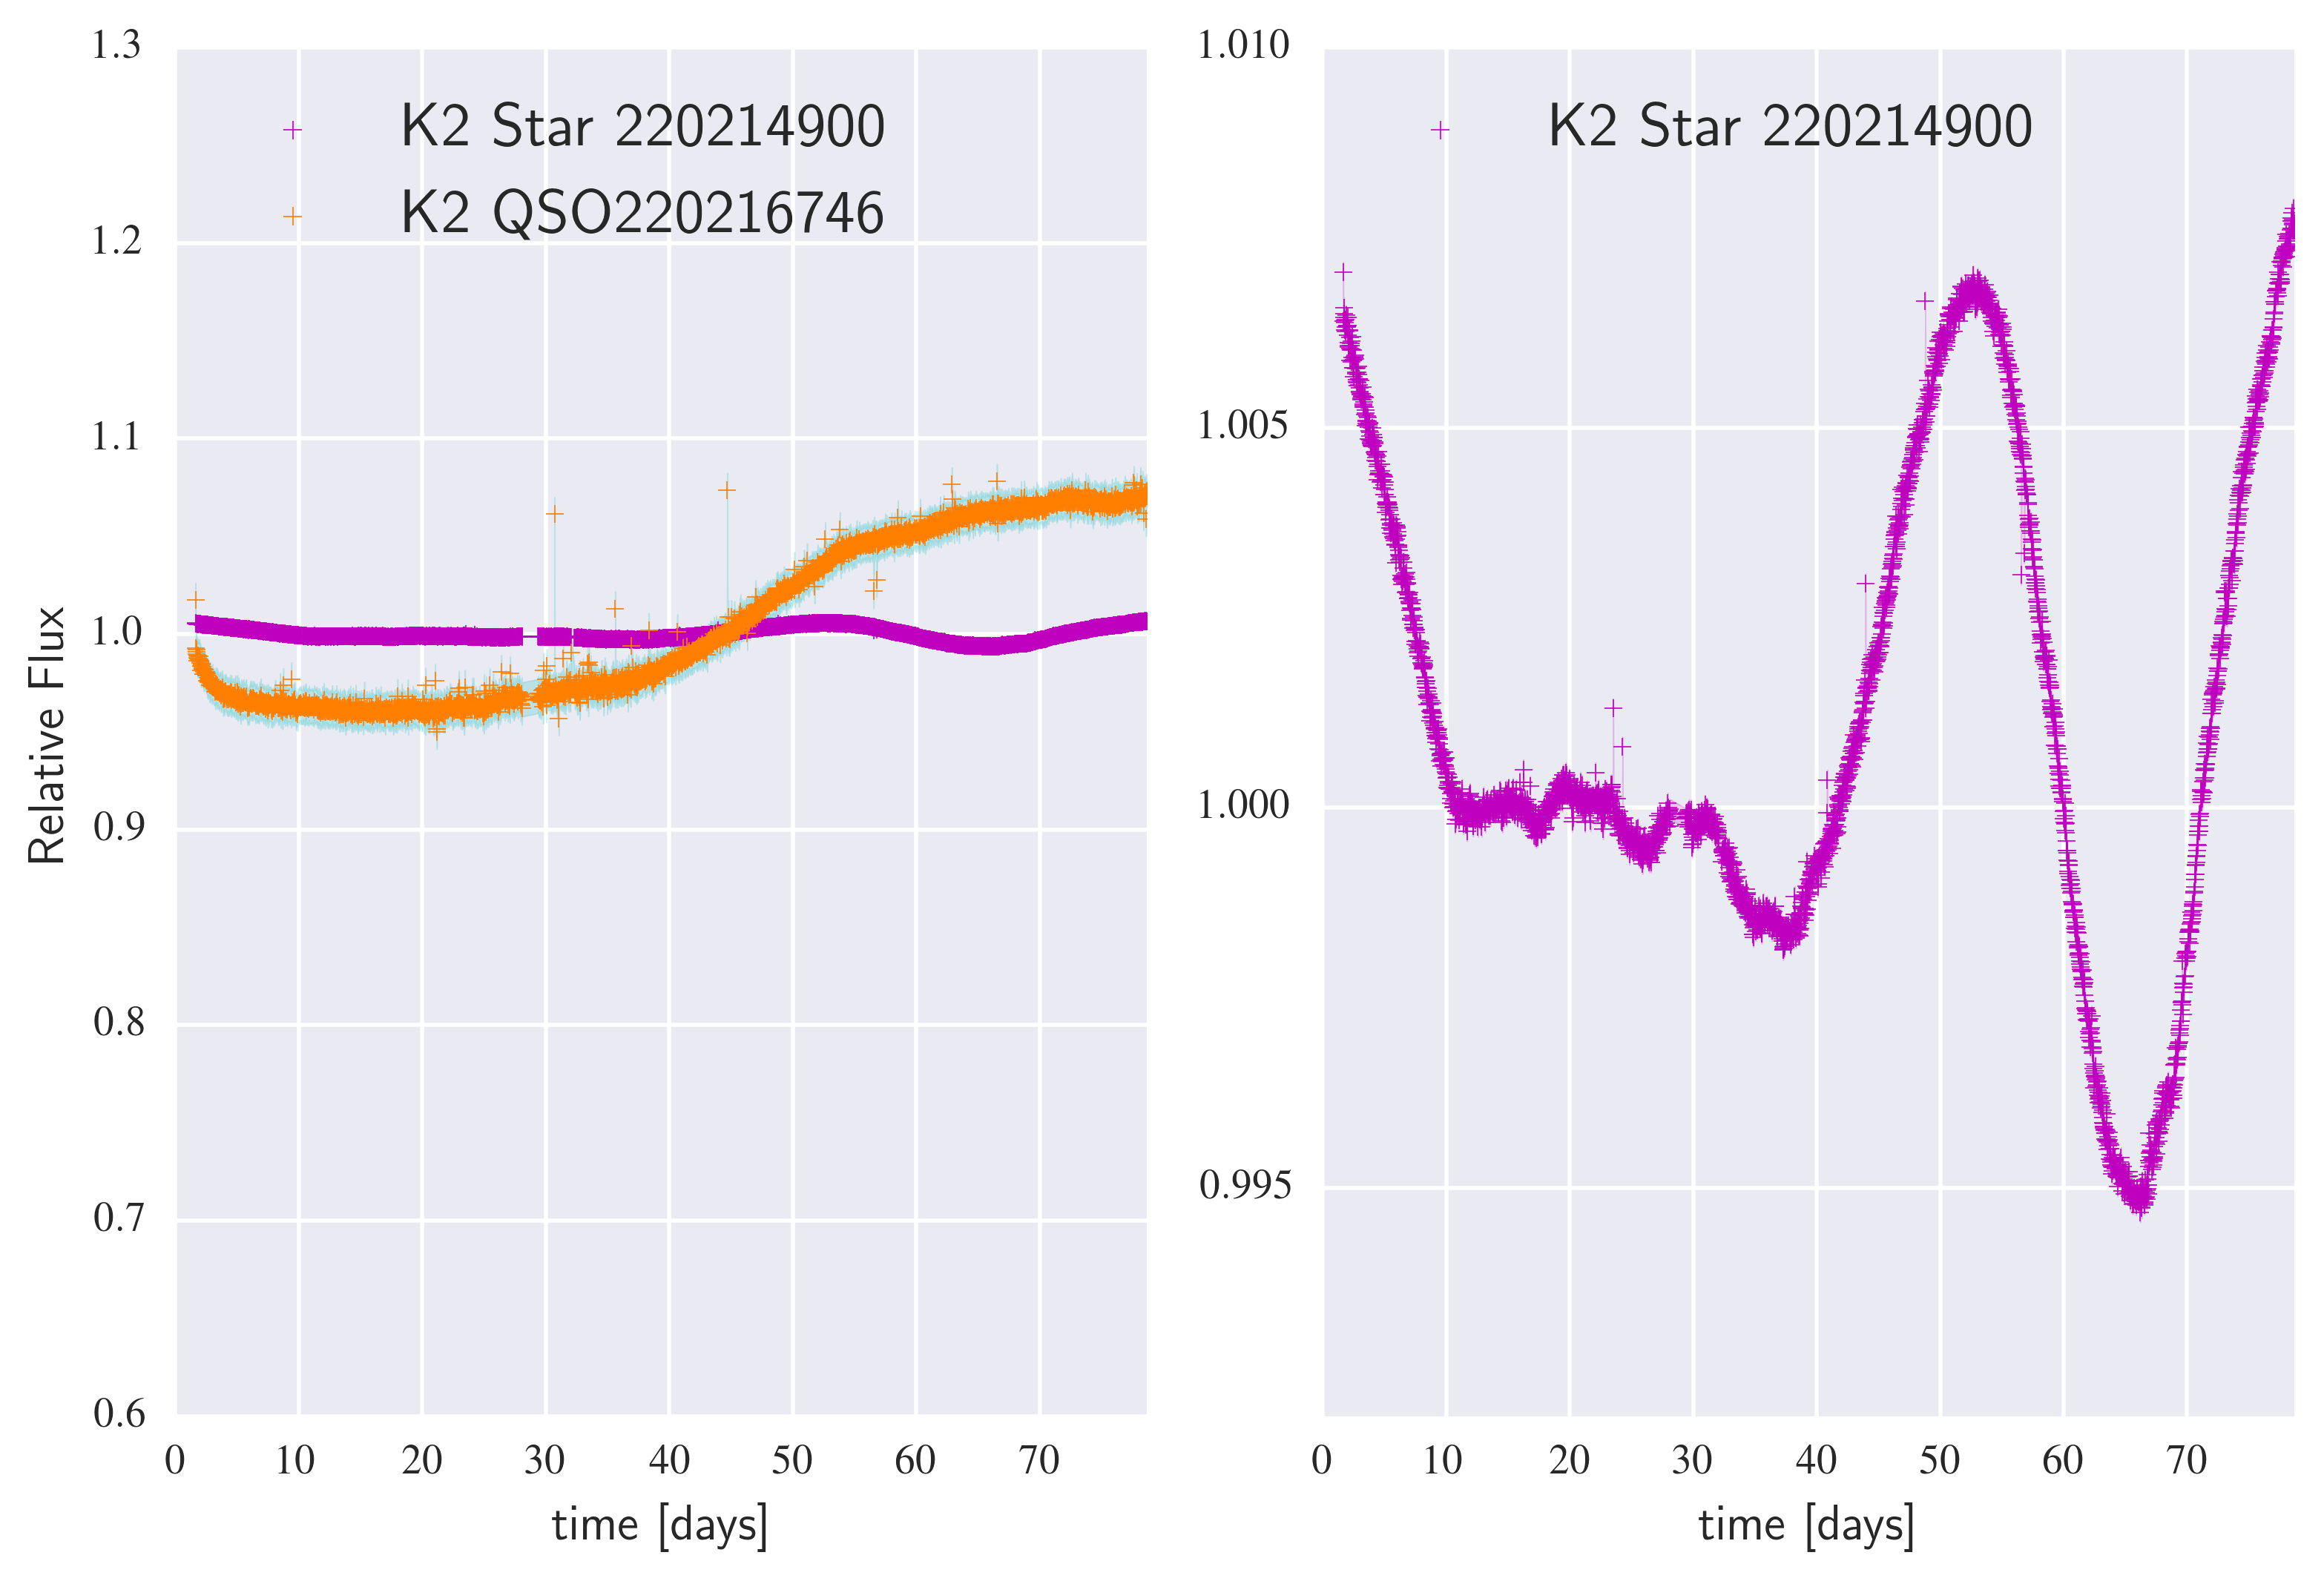
\includegraphics[width=\columnwidth]{220216746NearestNeighbor.png}
        		\caption{}
        		\label{fig:example_figure}
        	\end{figure}   
        	
        	\begin{figure}
        		% To include a figure from a file named example.*
        		% Allowable file formats are eps or ps if compiling using latex
        		% or pdf, png, jpg if compiling using pdflatex
 	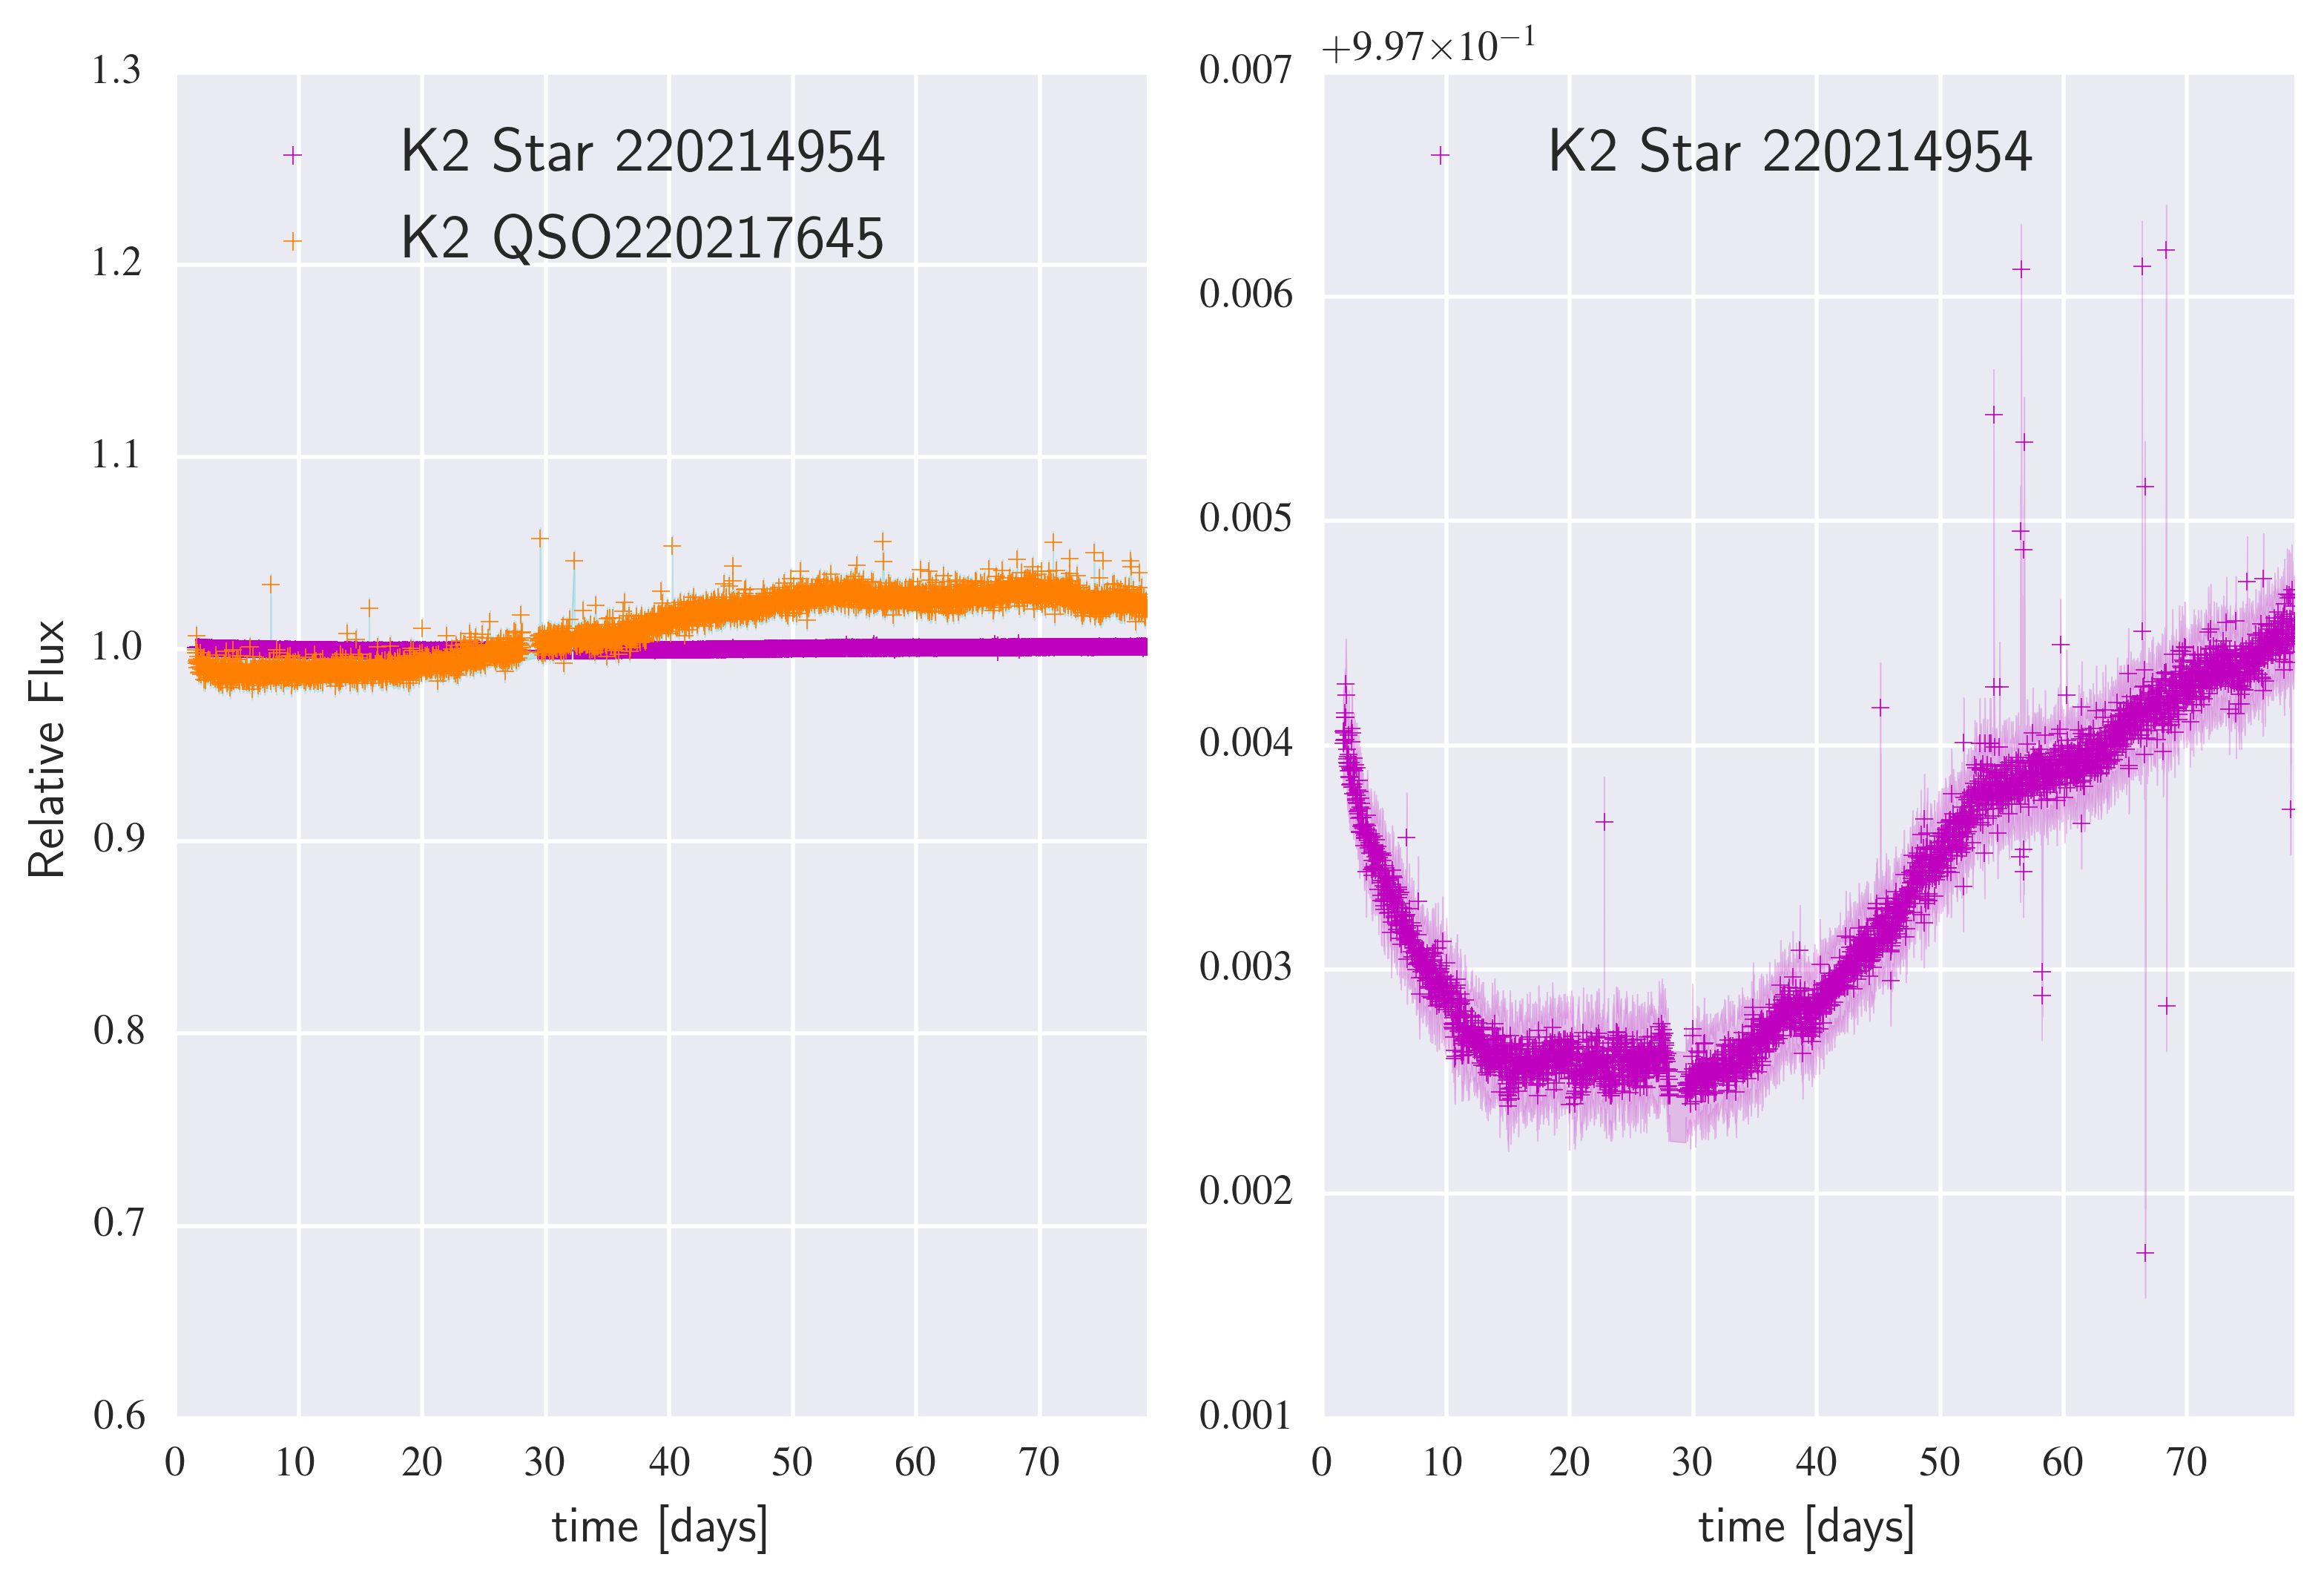
\includegraphics[width=\columnwidth]{220217645NearestNeighbor.png}
 	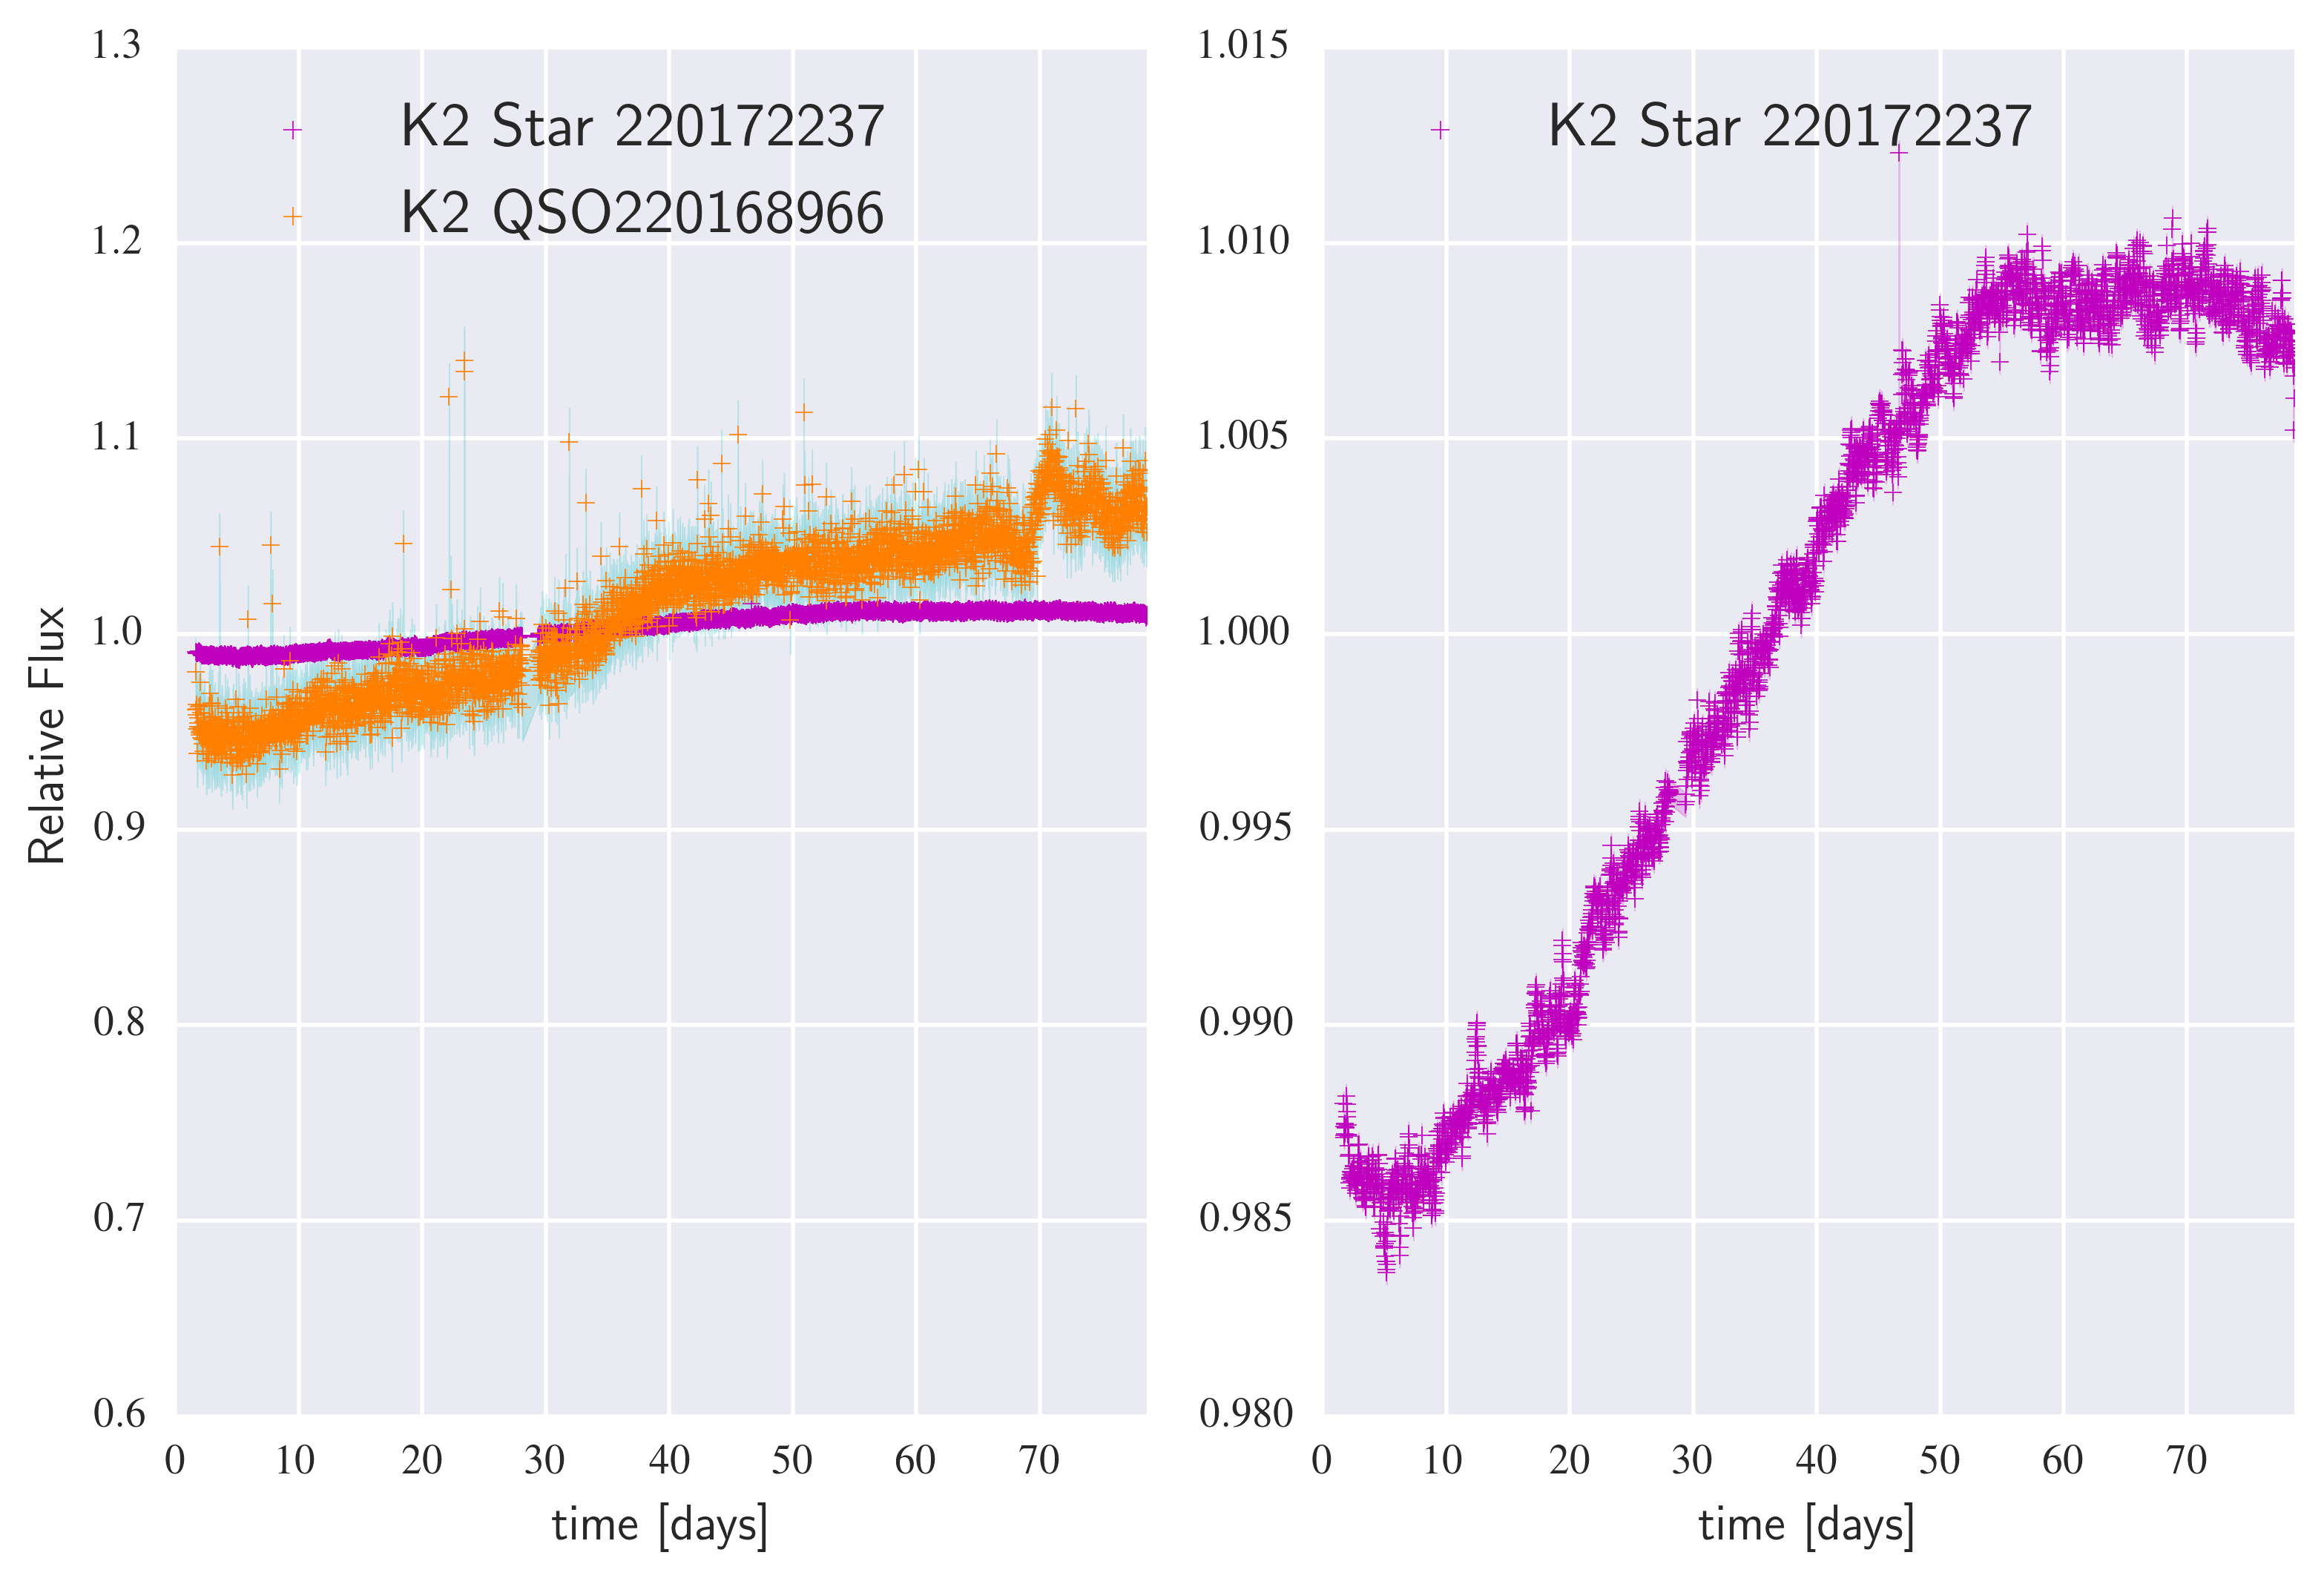
\includegraphics[width=\columnwidth]{220168966NearestNeighbor.png}
 	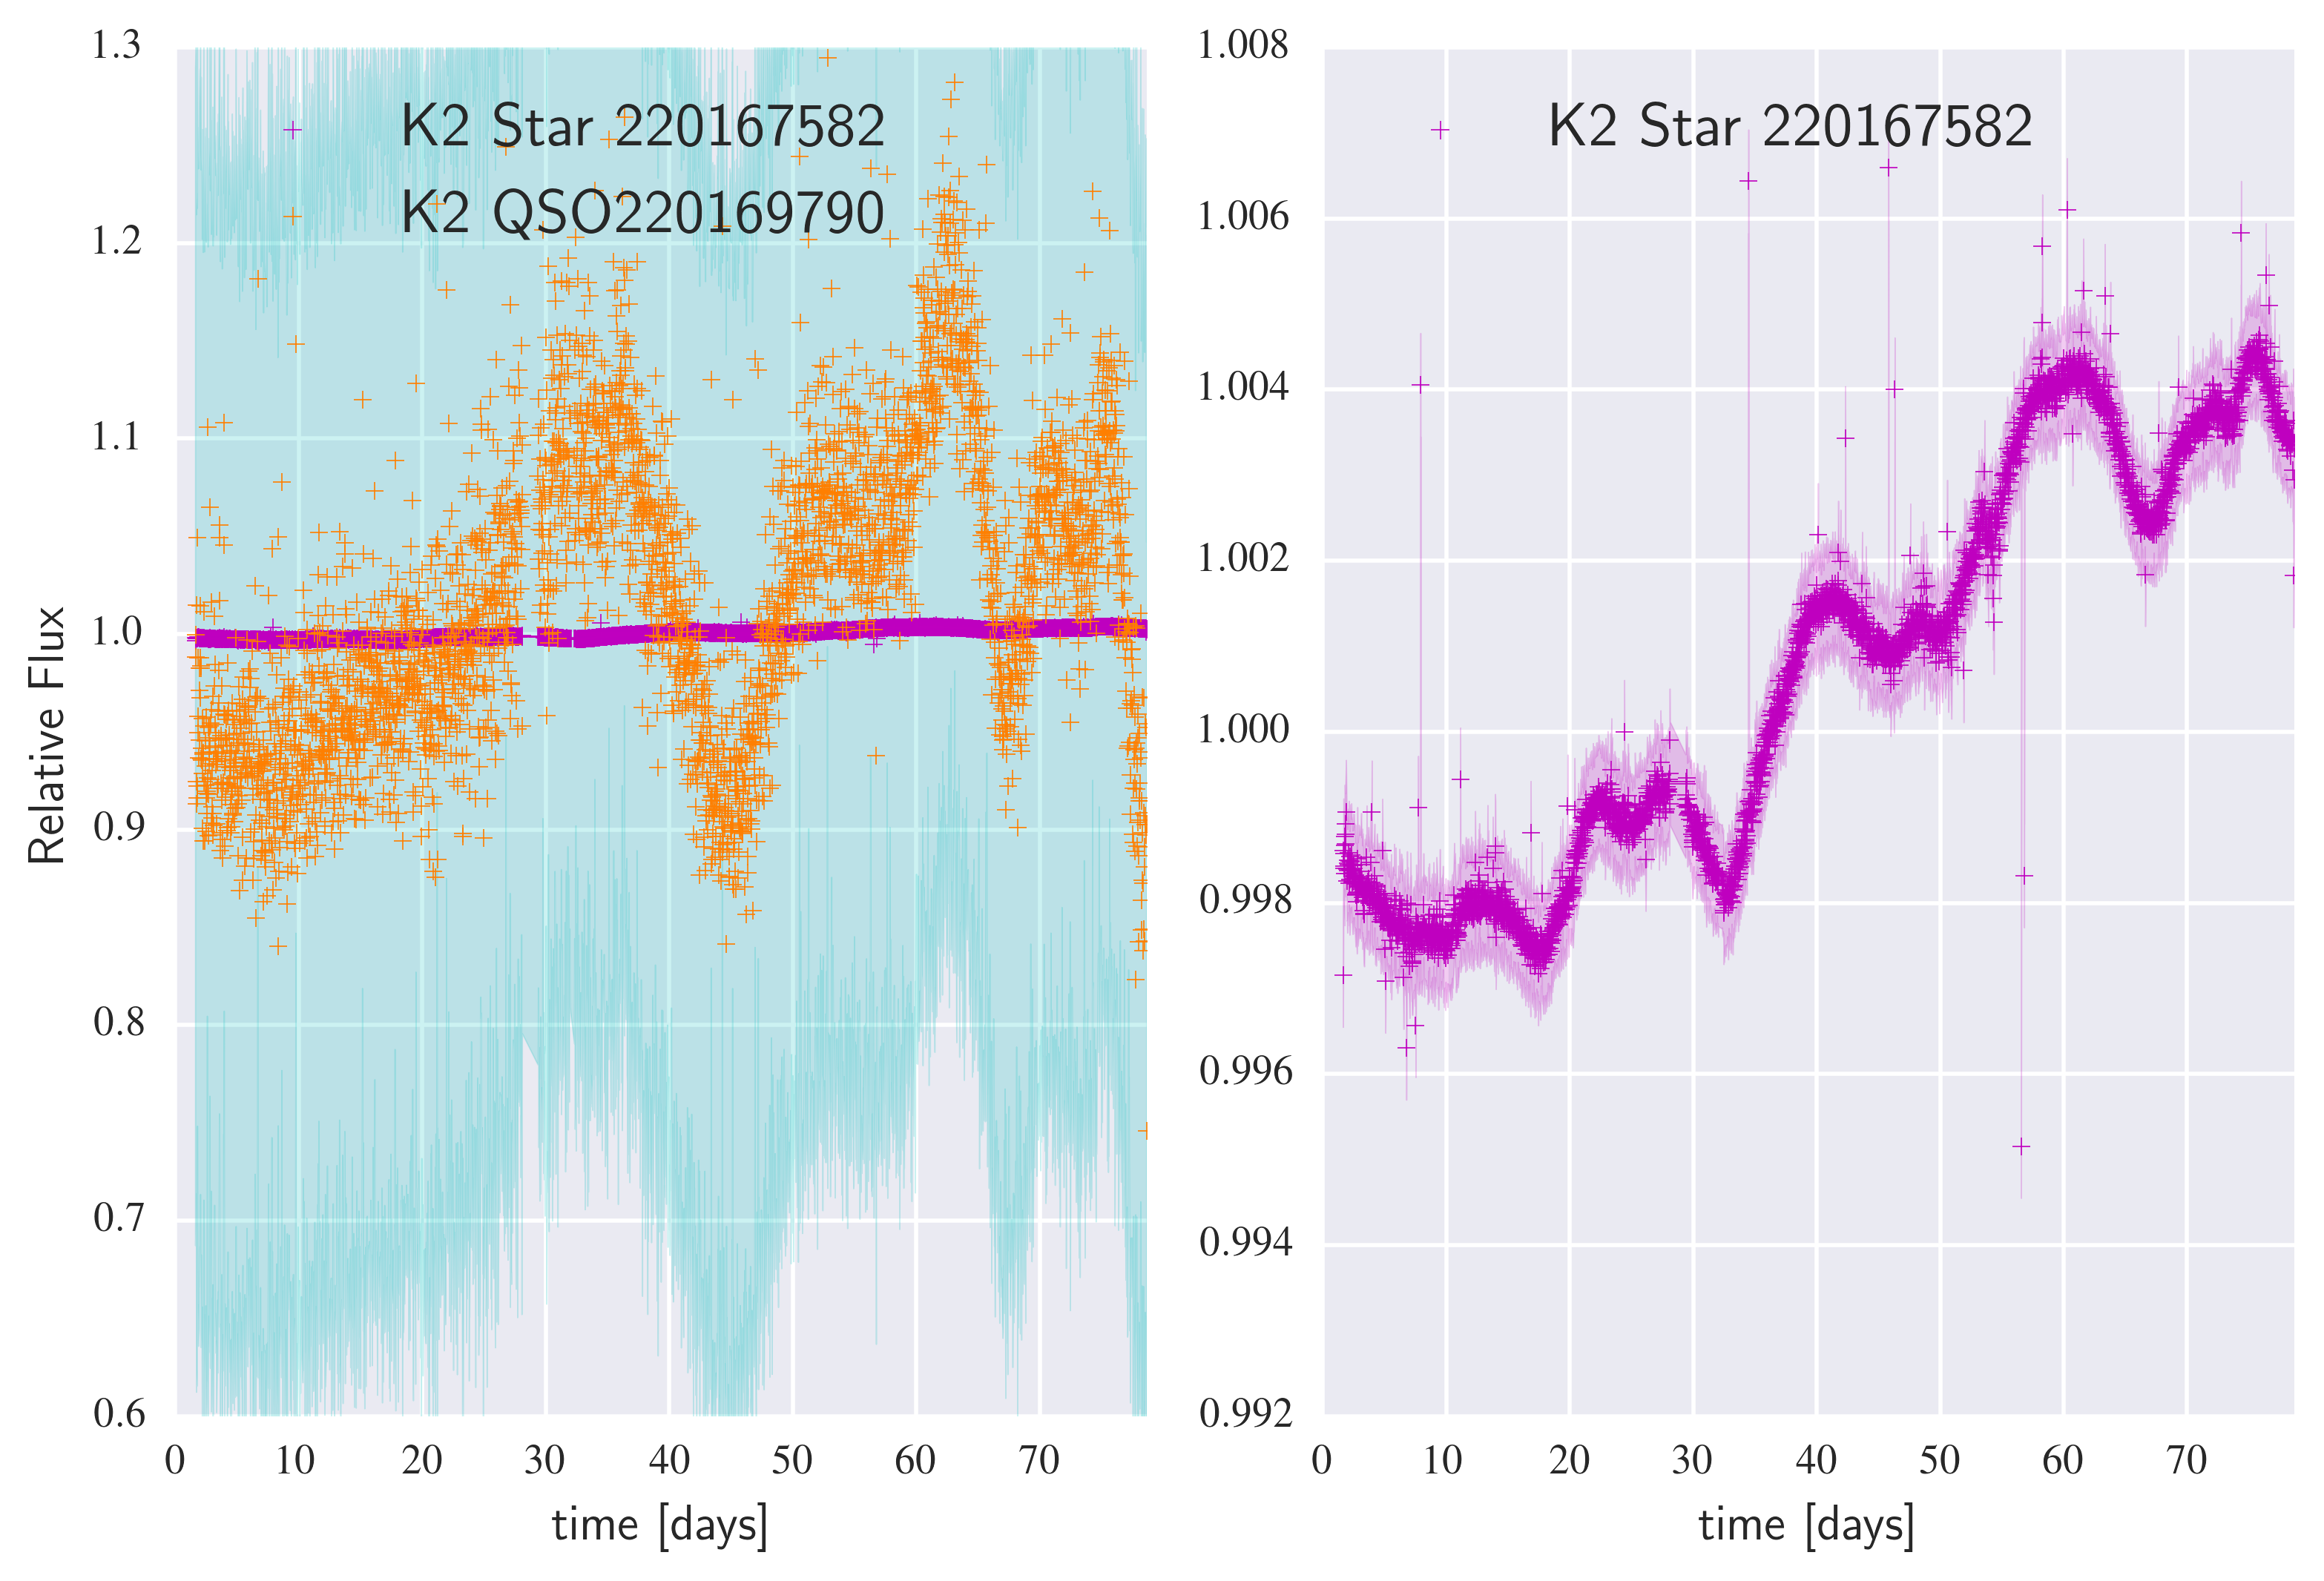
\includegraphics[width=\columnwidth]{220169790NearestNeighbor.png}
        		\caption{}
        		\label{fig:example_figure}
        	\end{figure}   
        	
        	
         	\begin{figure}
         		% To include a figure from a file named example.*
         		% Allowable file formats are eps or ps if compiling using latex
         		% or pdf, png, jpg if compiling using pdflatex
 	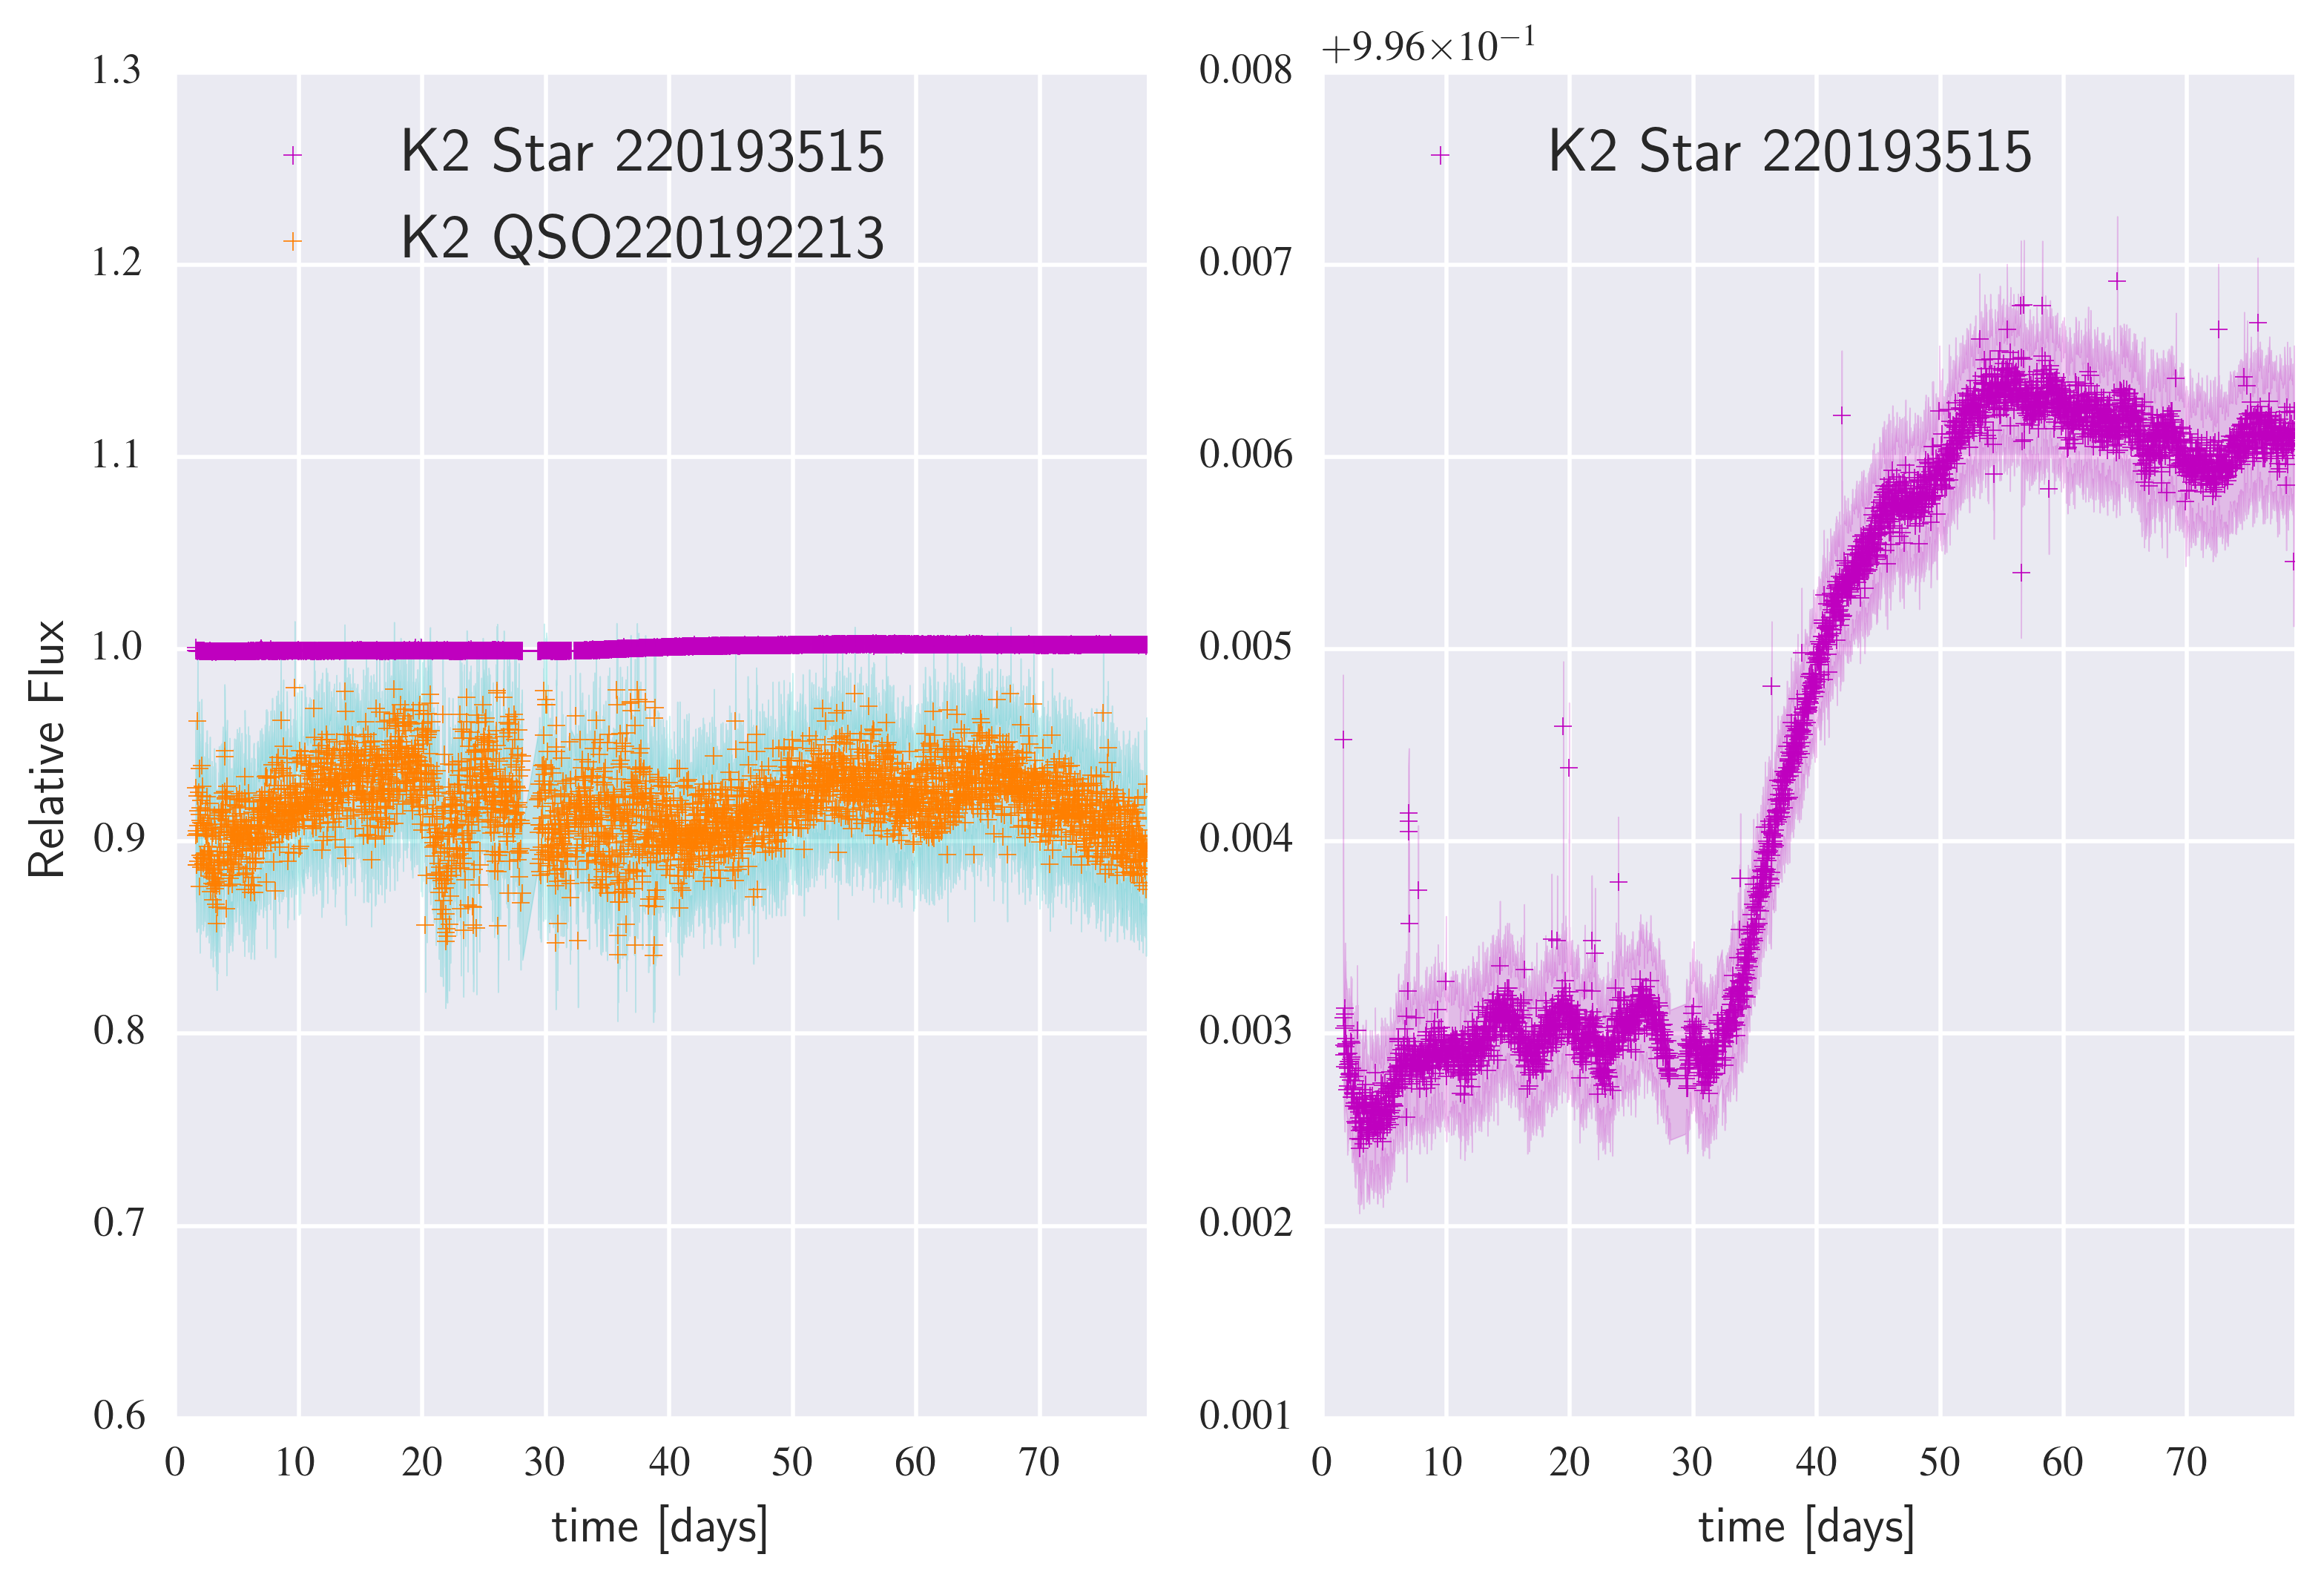
\includegraphics[width=\columnwidth]{220192213NearestNeighbor.png}
 	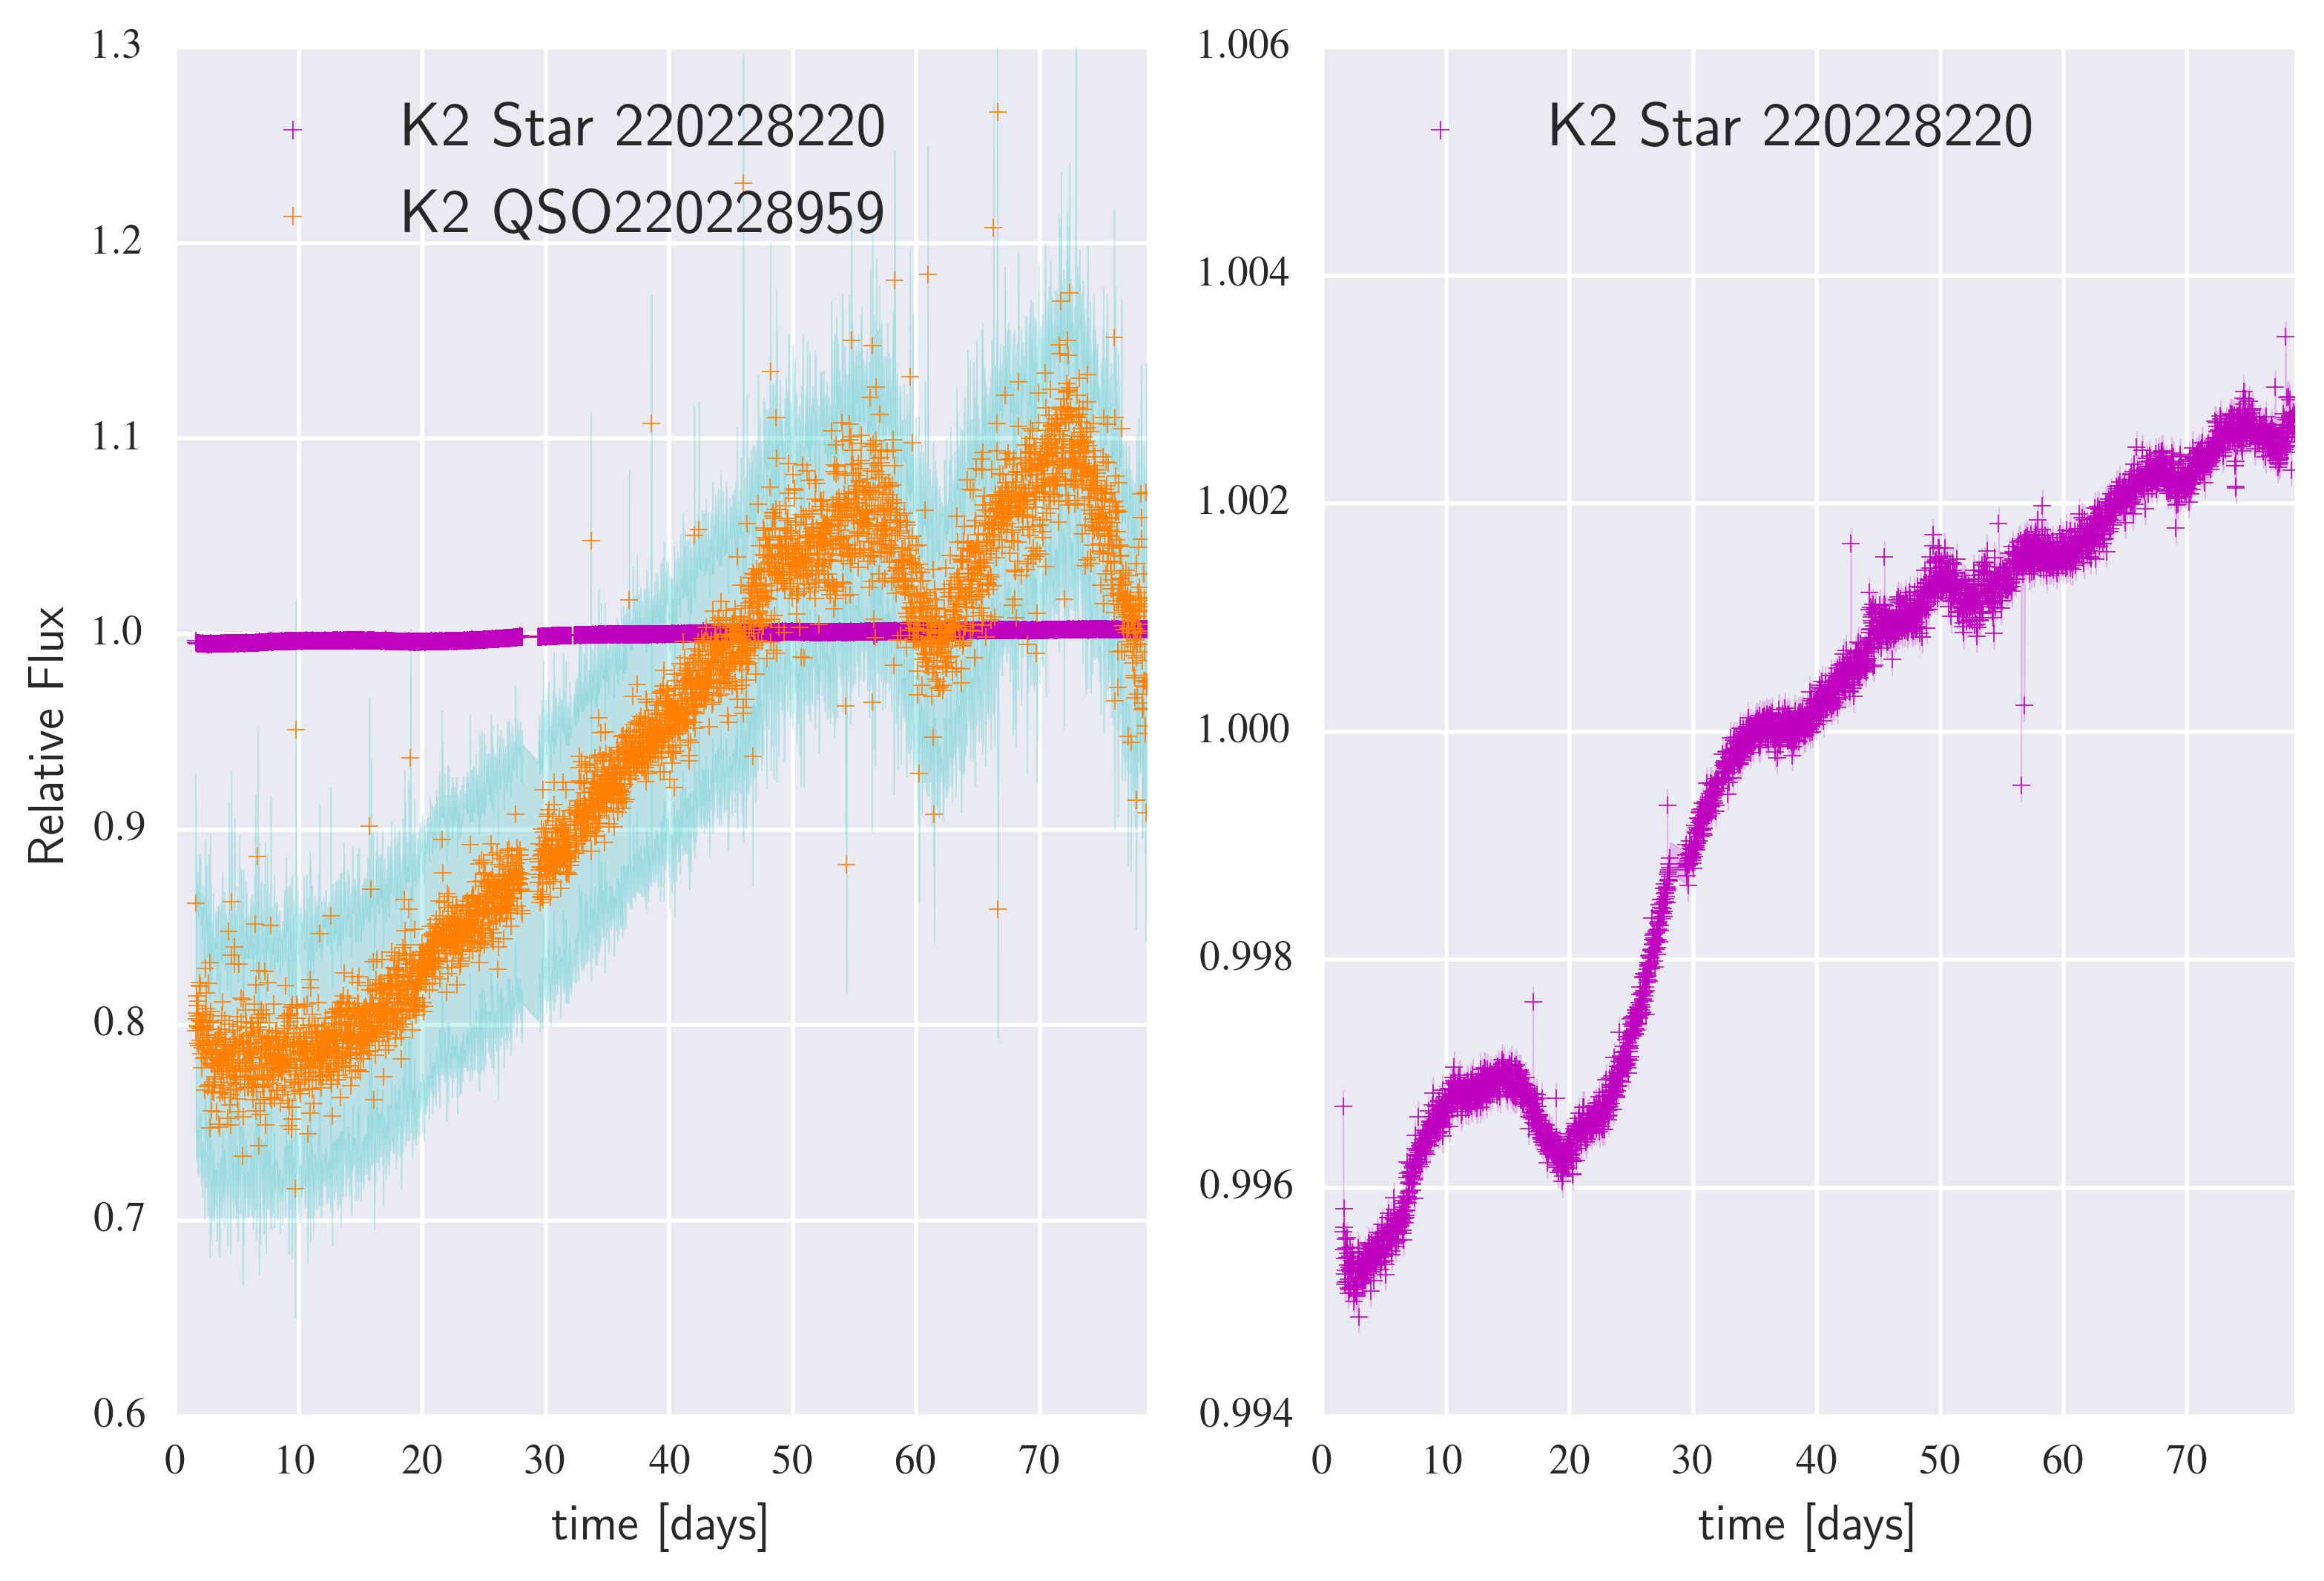
\includegraphics[width=\columnwidth]{220228959NearestNeighbor.png}
 	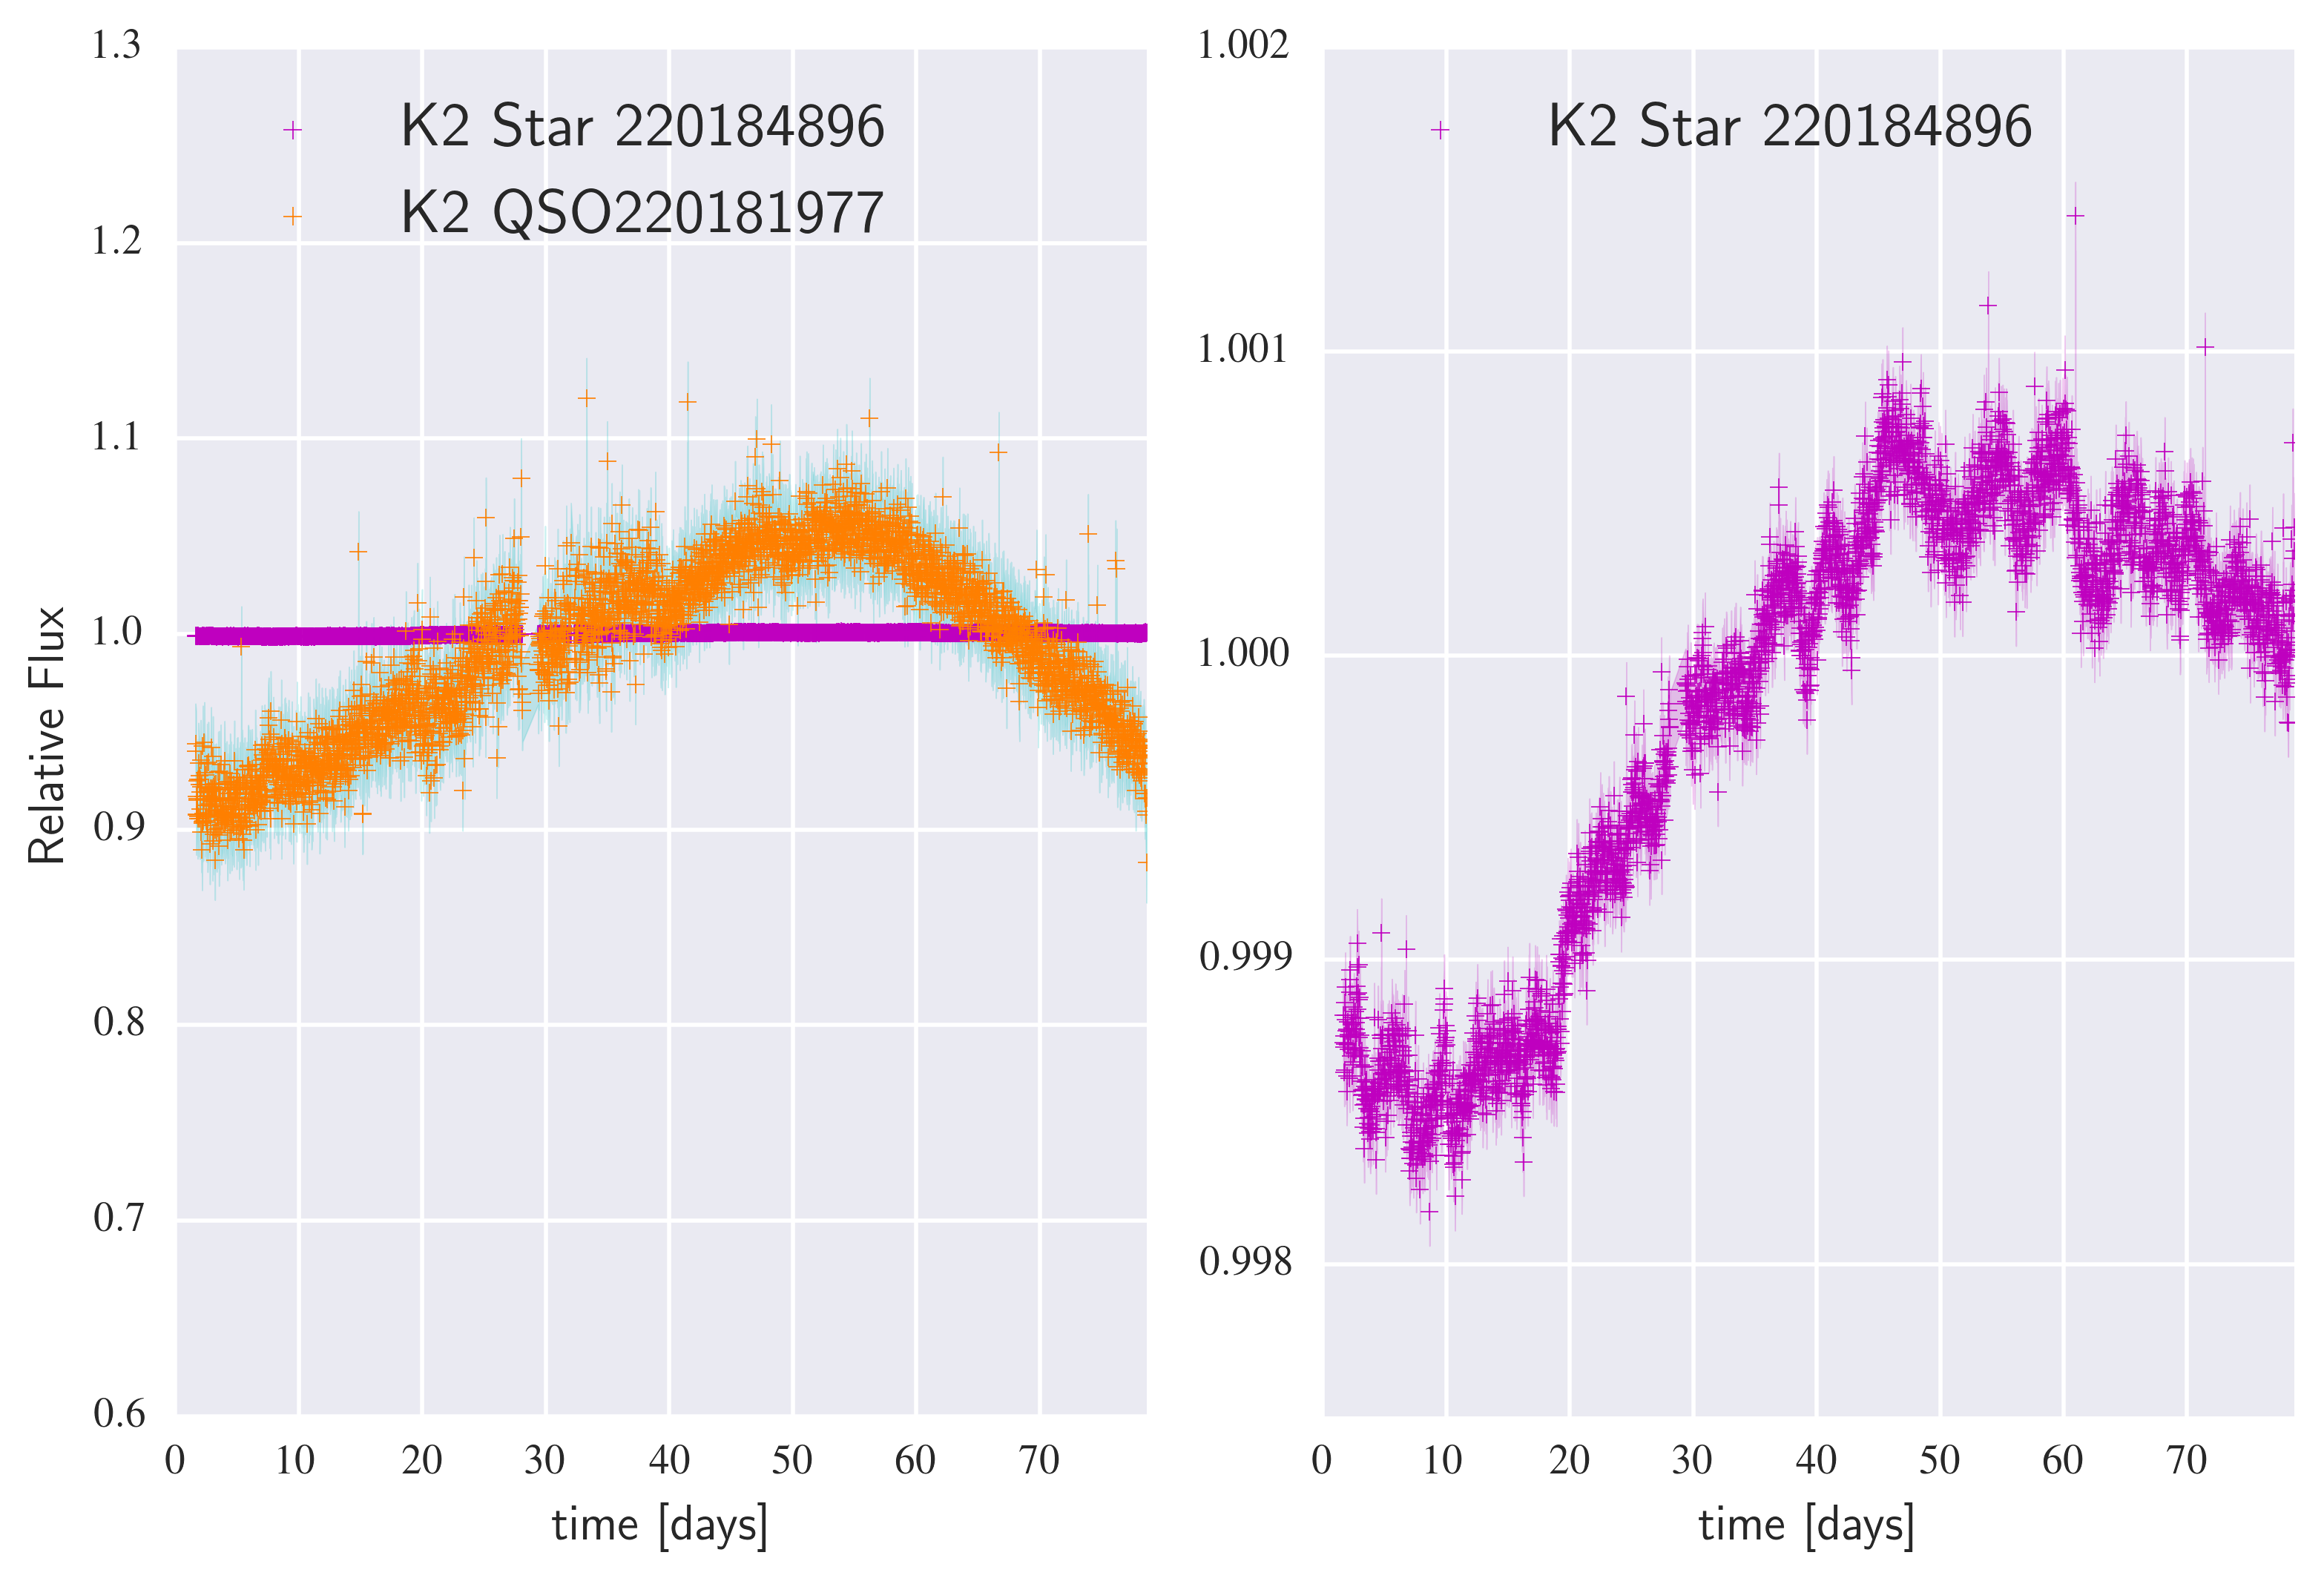
\includegraphics[width=\columnwidth]{220181977NearestNeighbor.png}
         		\caption{}
         		\label{fig:example_figure}
         	\end{figure}          	
        	\begin{figure}
        		% To include a figure from a file named example.*
        		% Allowable file formats are eps or ps if compiling using latex
        		% or pdf, png, jpg if compiling using pdflatex
 	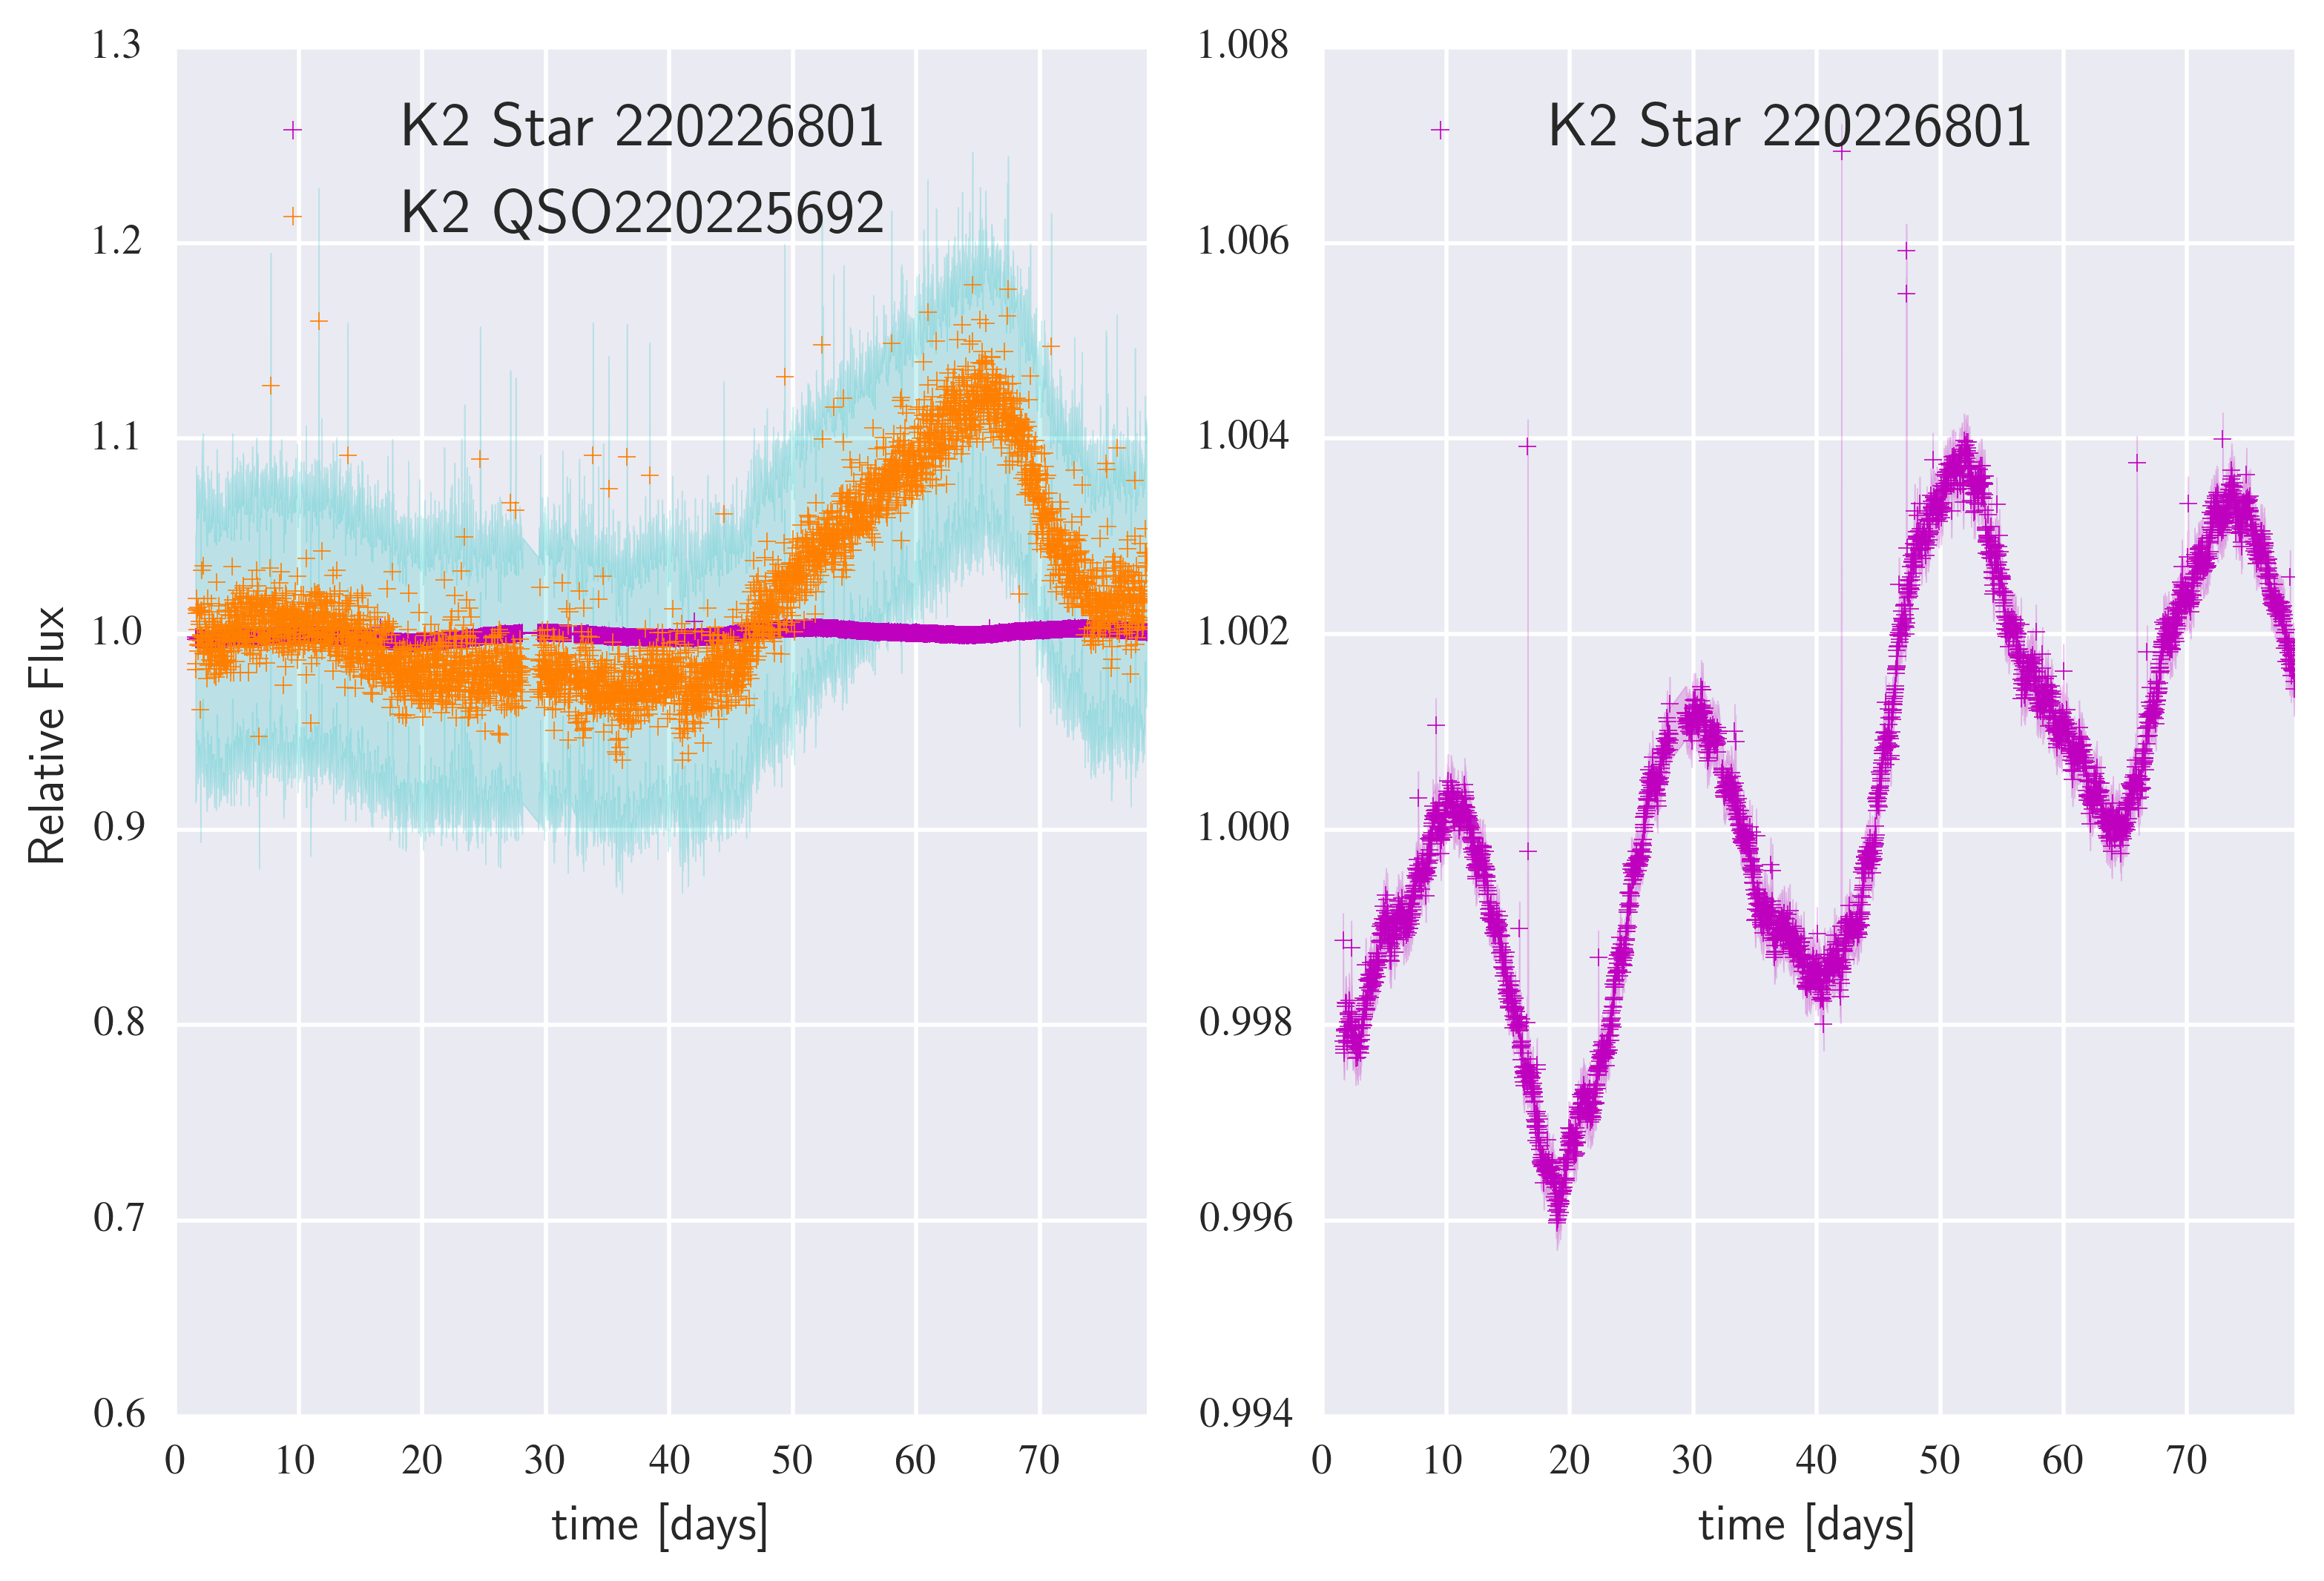
\includegraphics[width=\columnwidth]{220225692NearestNeighbor.png}
 	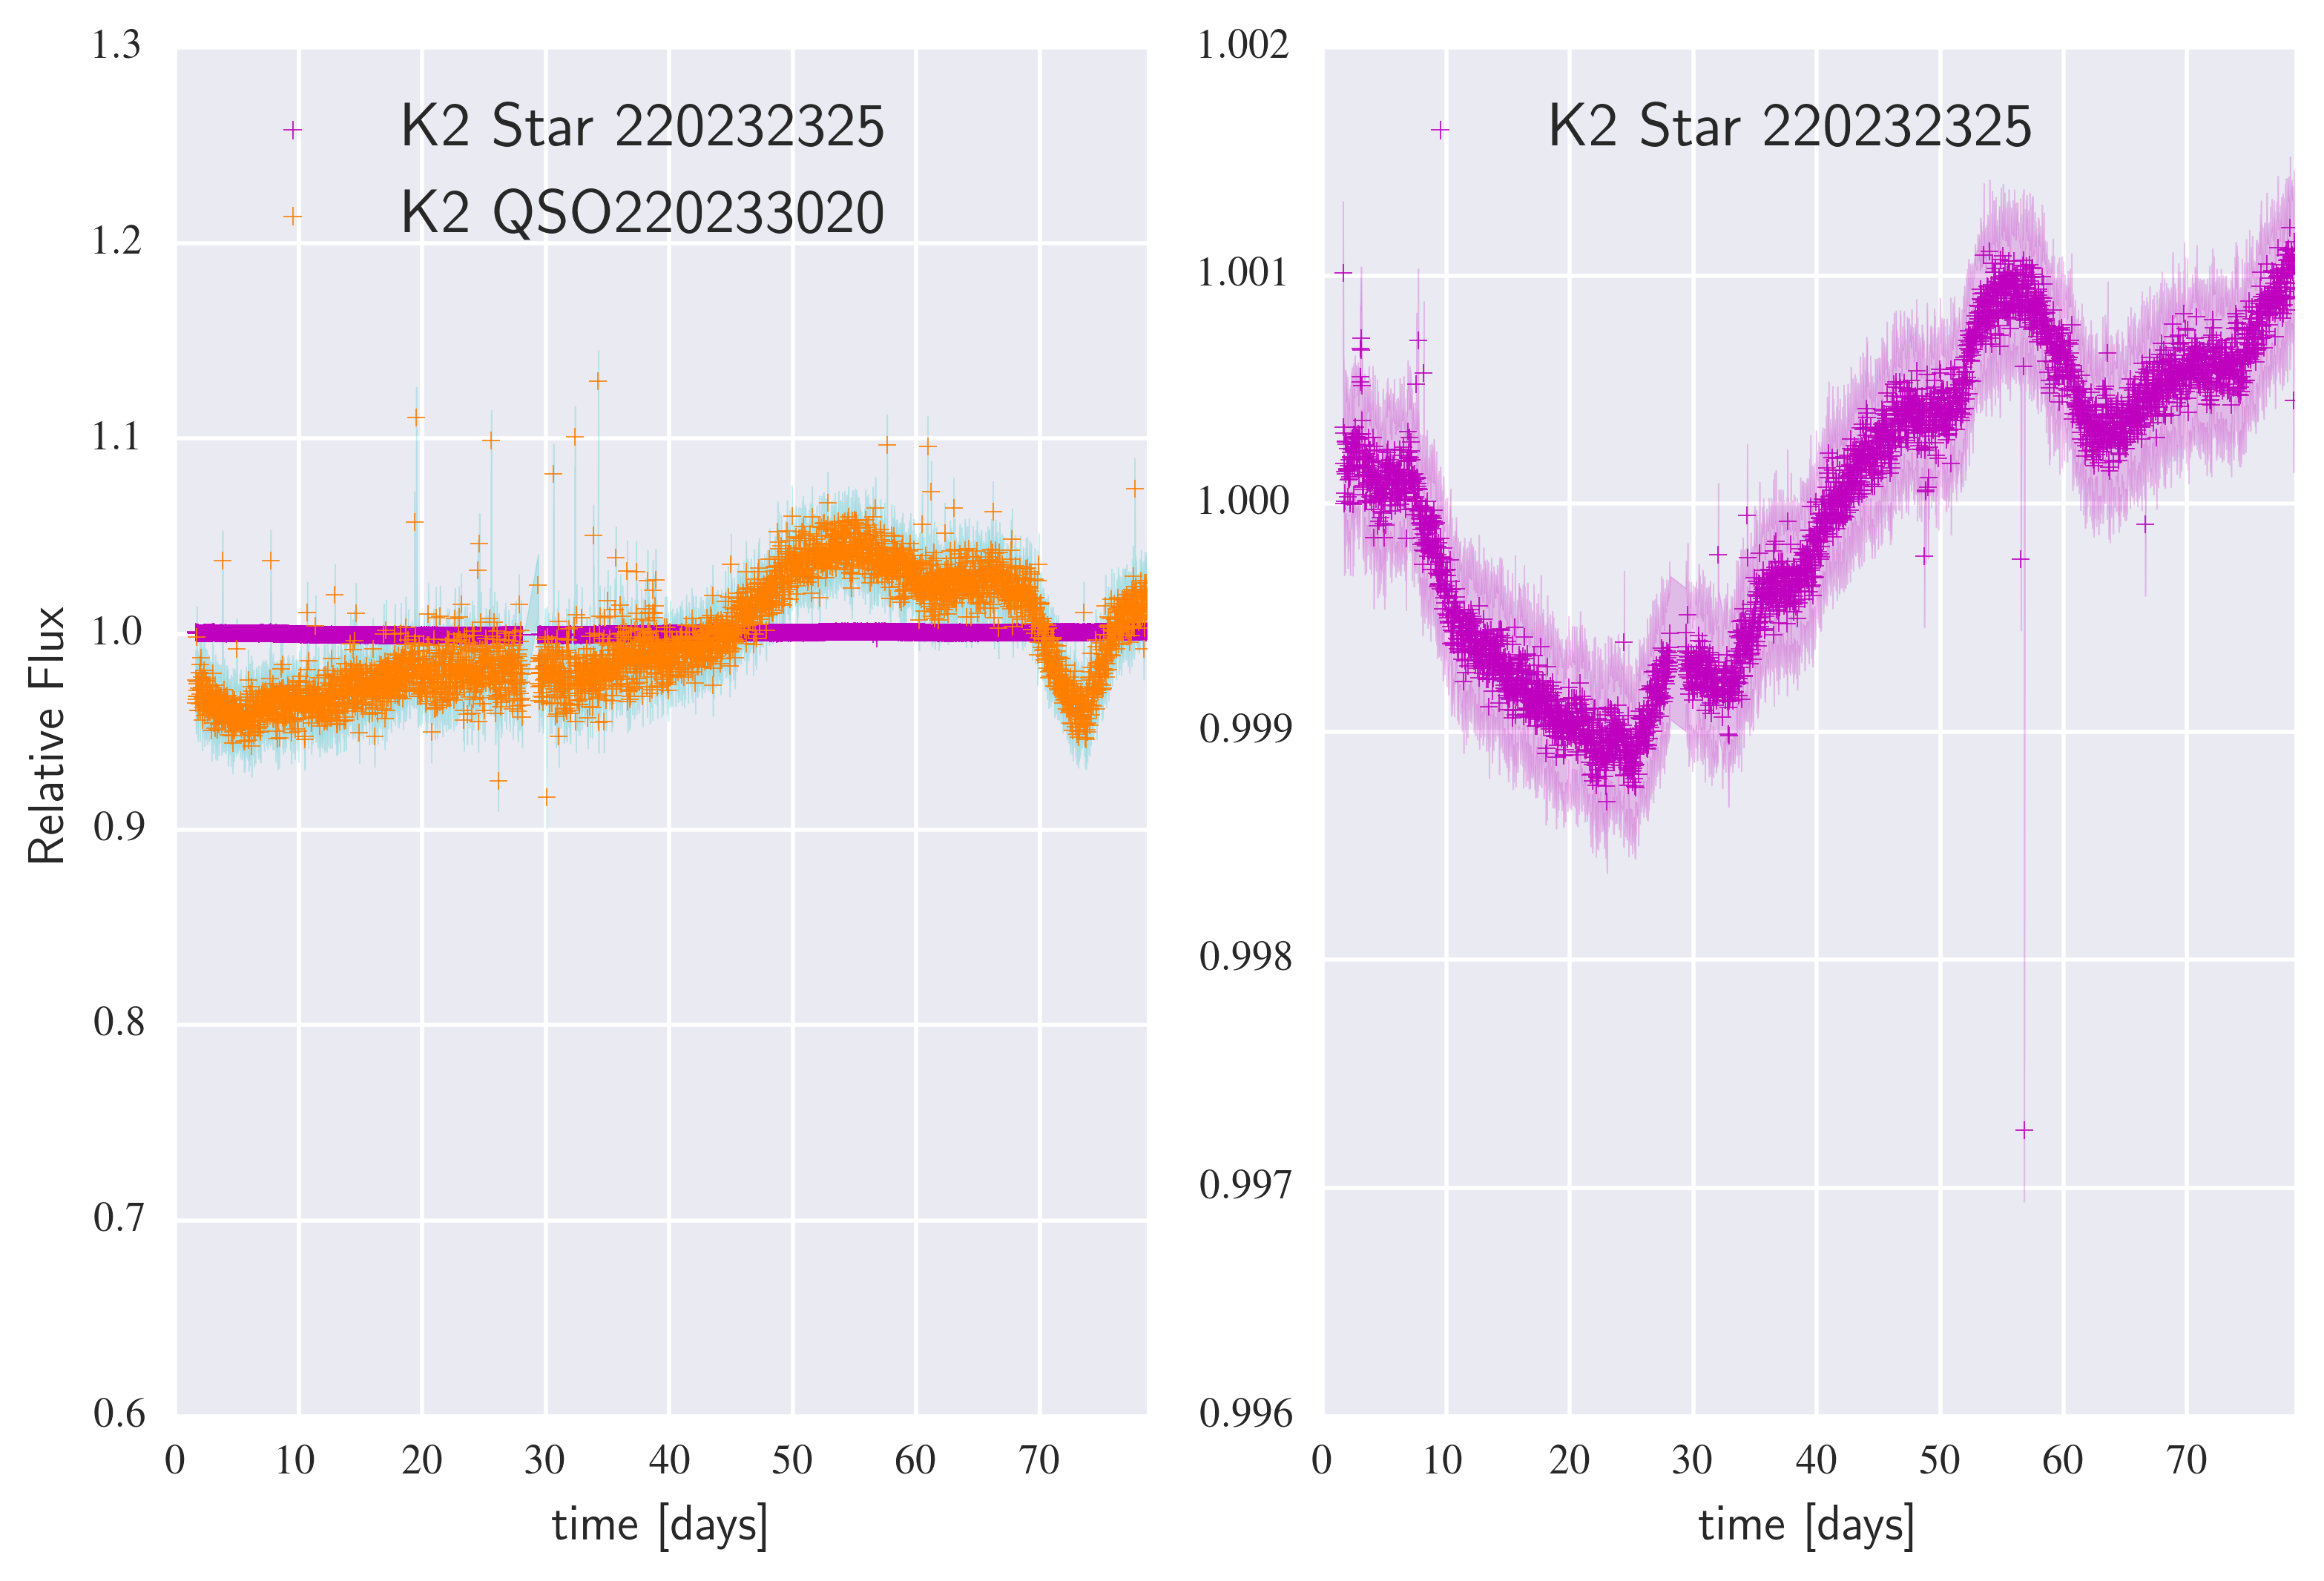
\includegraphics[width=\columnwidth]{220233020NearestNeighbor.png}
 	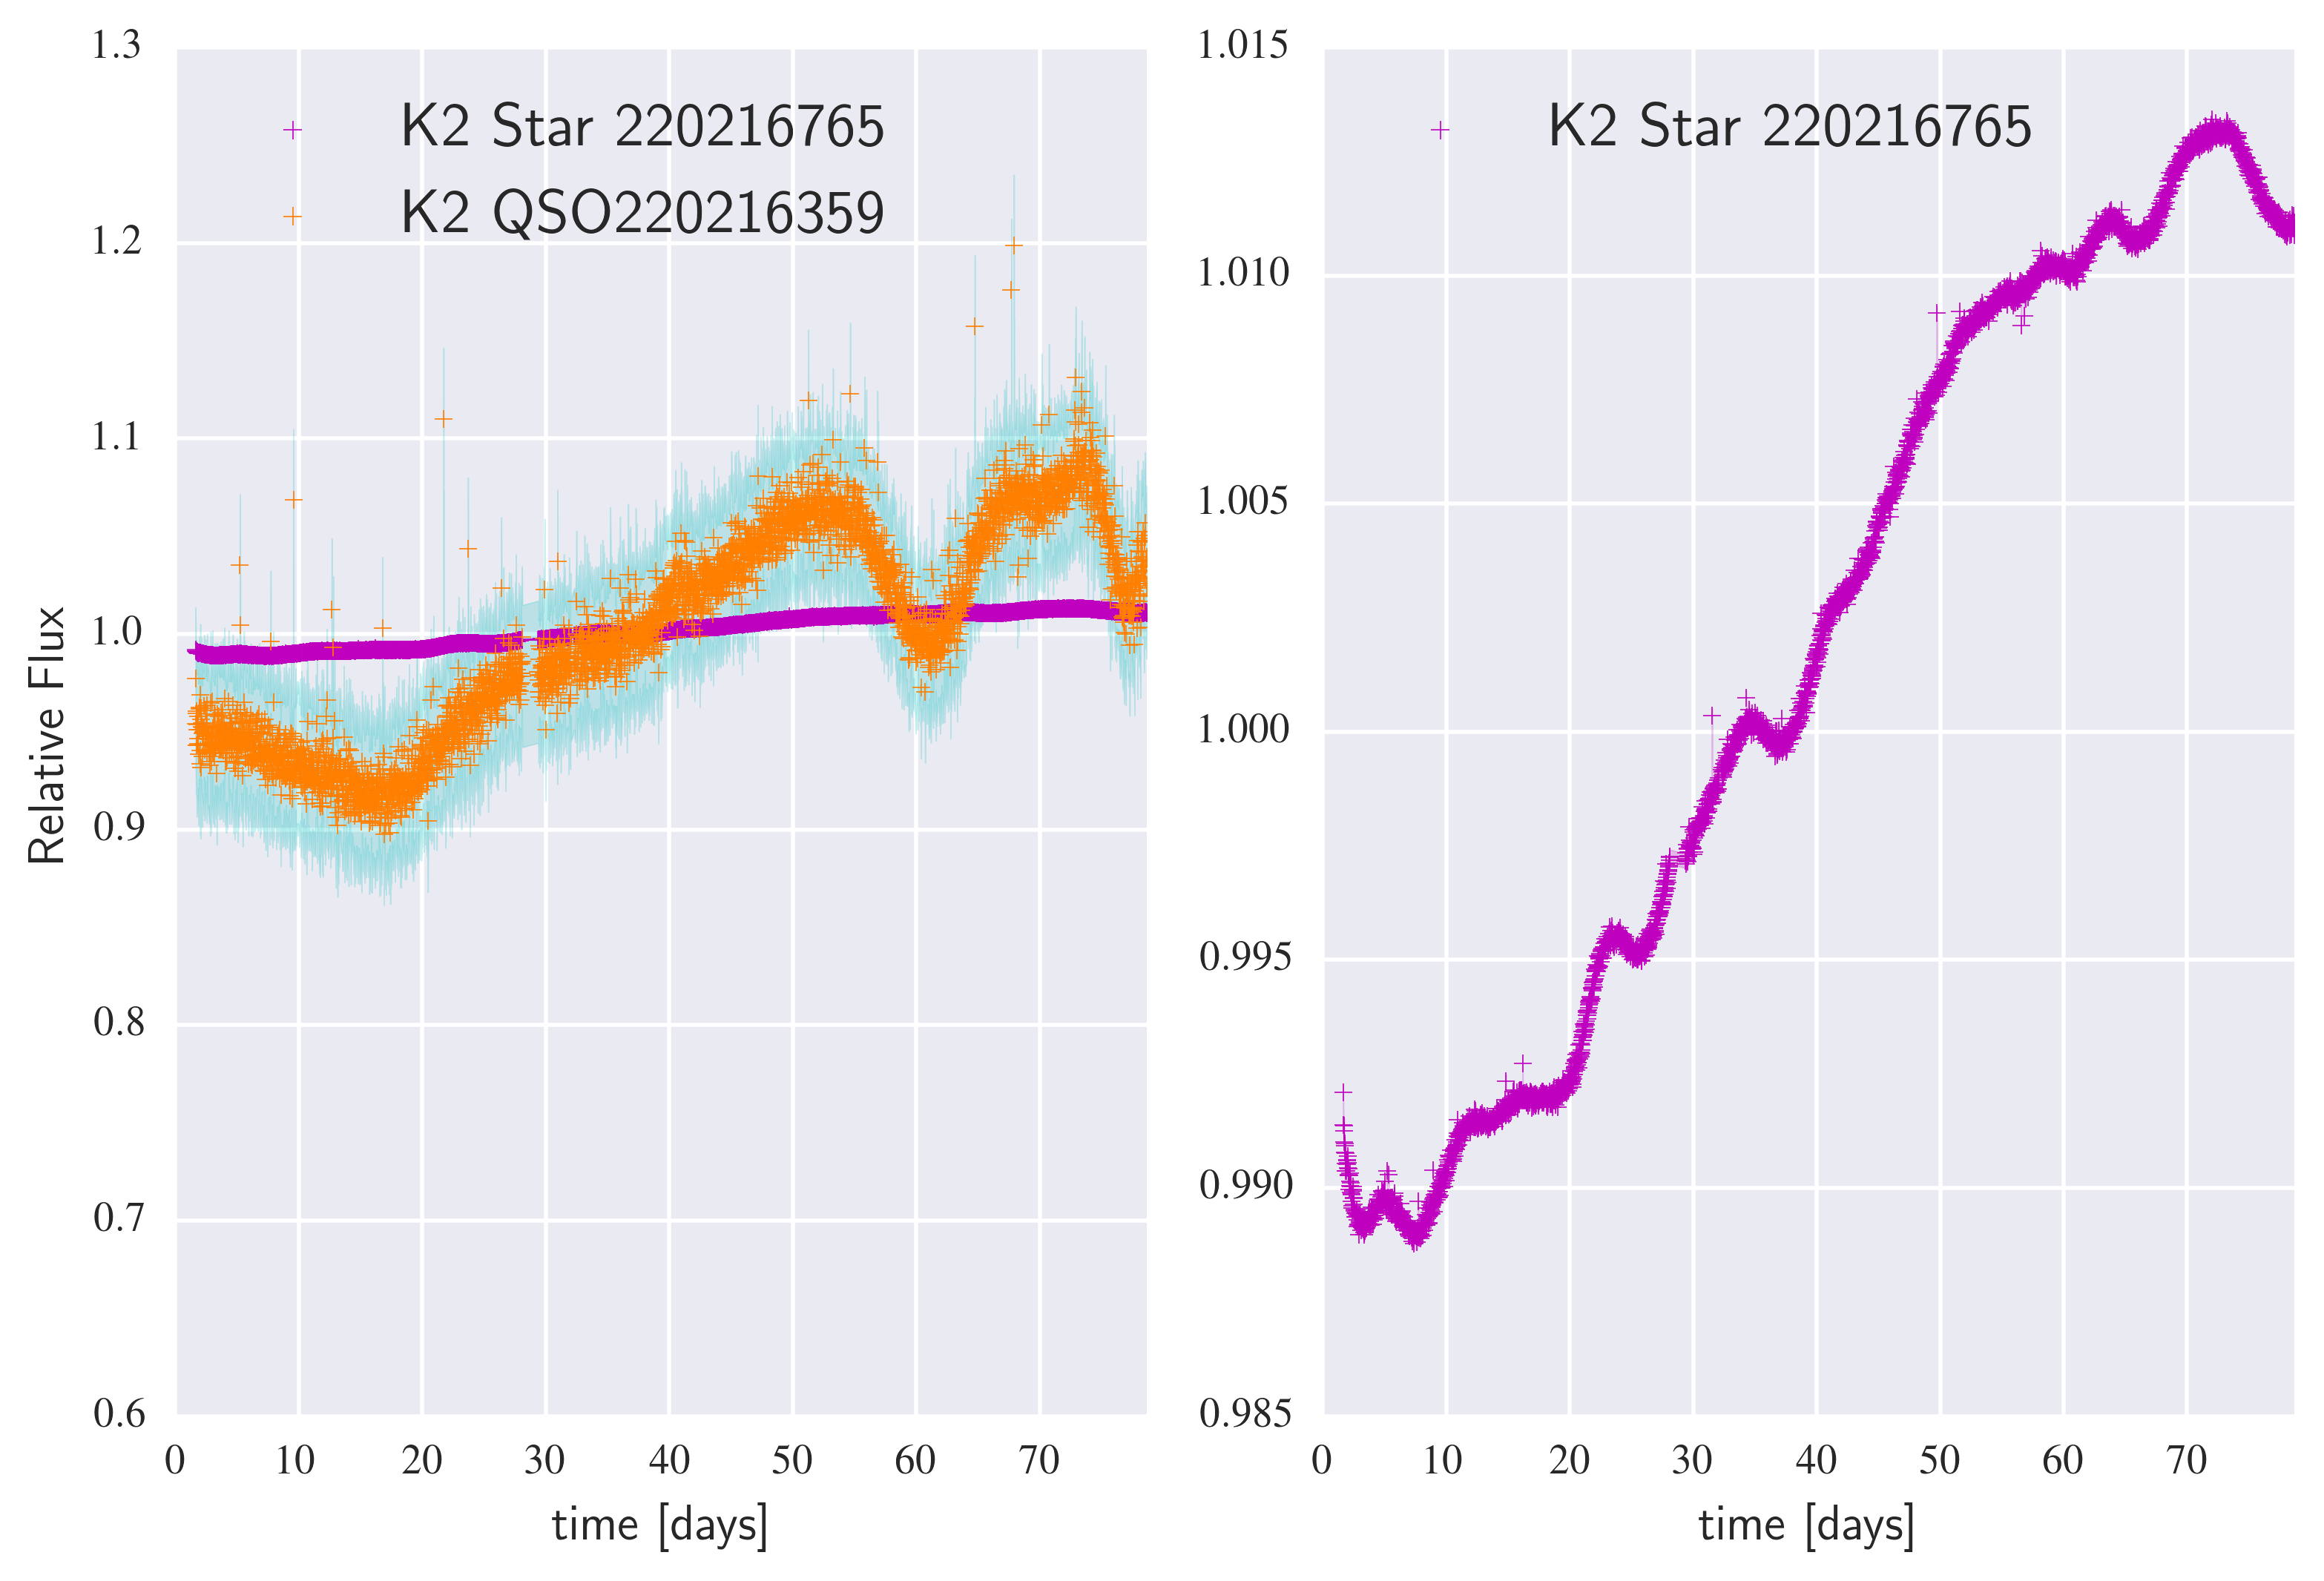
\includegraphics[width=\columnwidth]{220216359NearestNeighbor.png}
        		\caption{}
        		\label{fig:example_figure}
        	\end{figure}           	
        	
        	\begin{figure}
        	% To include a figure from a file named example.*
        	% Allowable file formats are eps or ps if compiling using latex
        	% or pdf, png, jpg if compiling using pdflatex
 	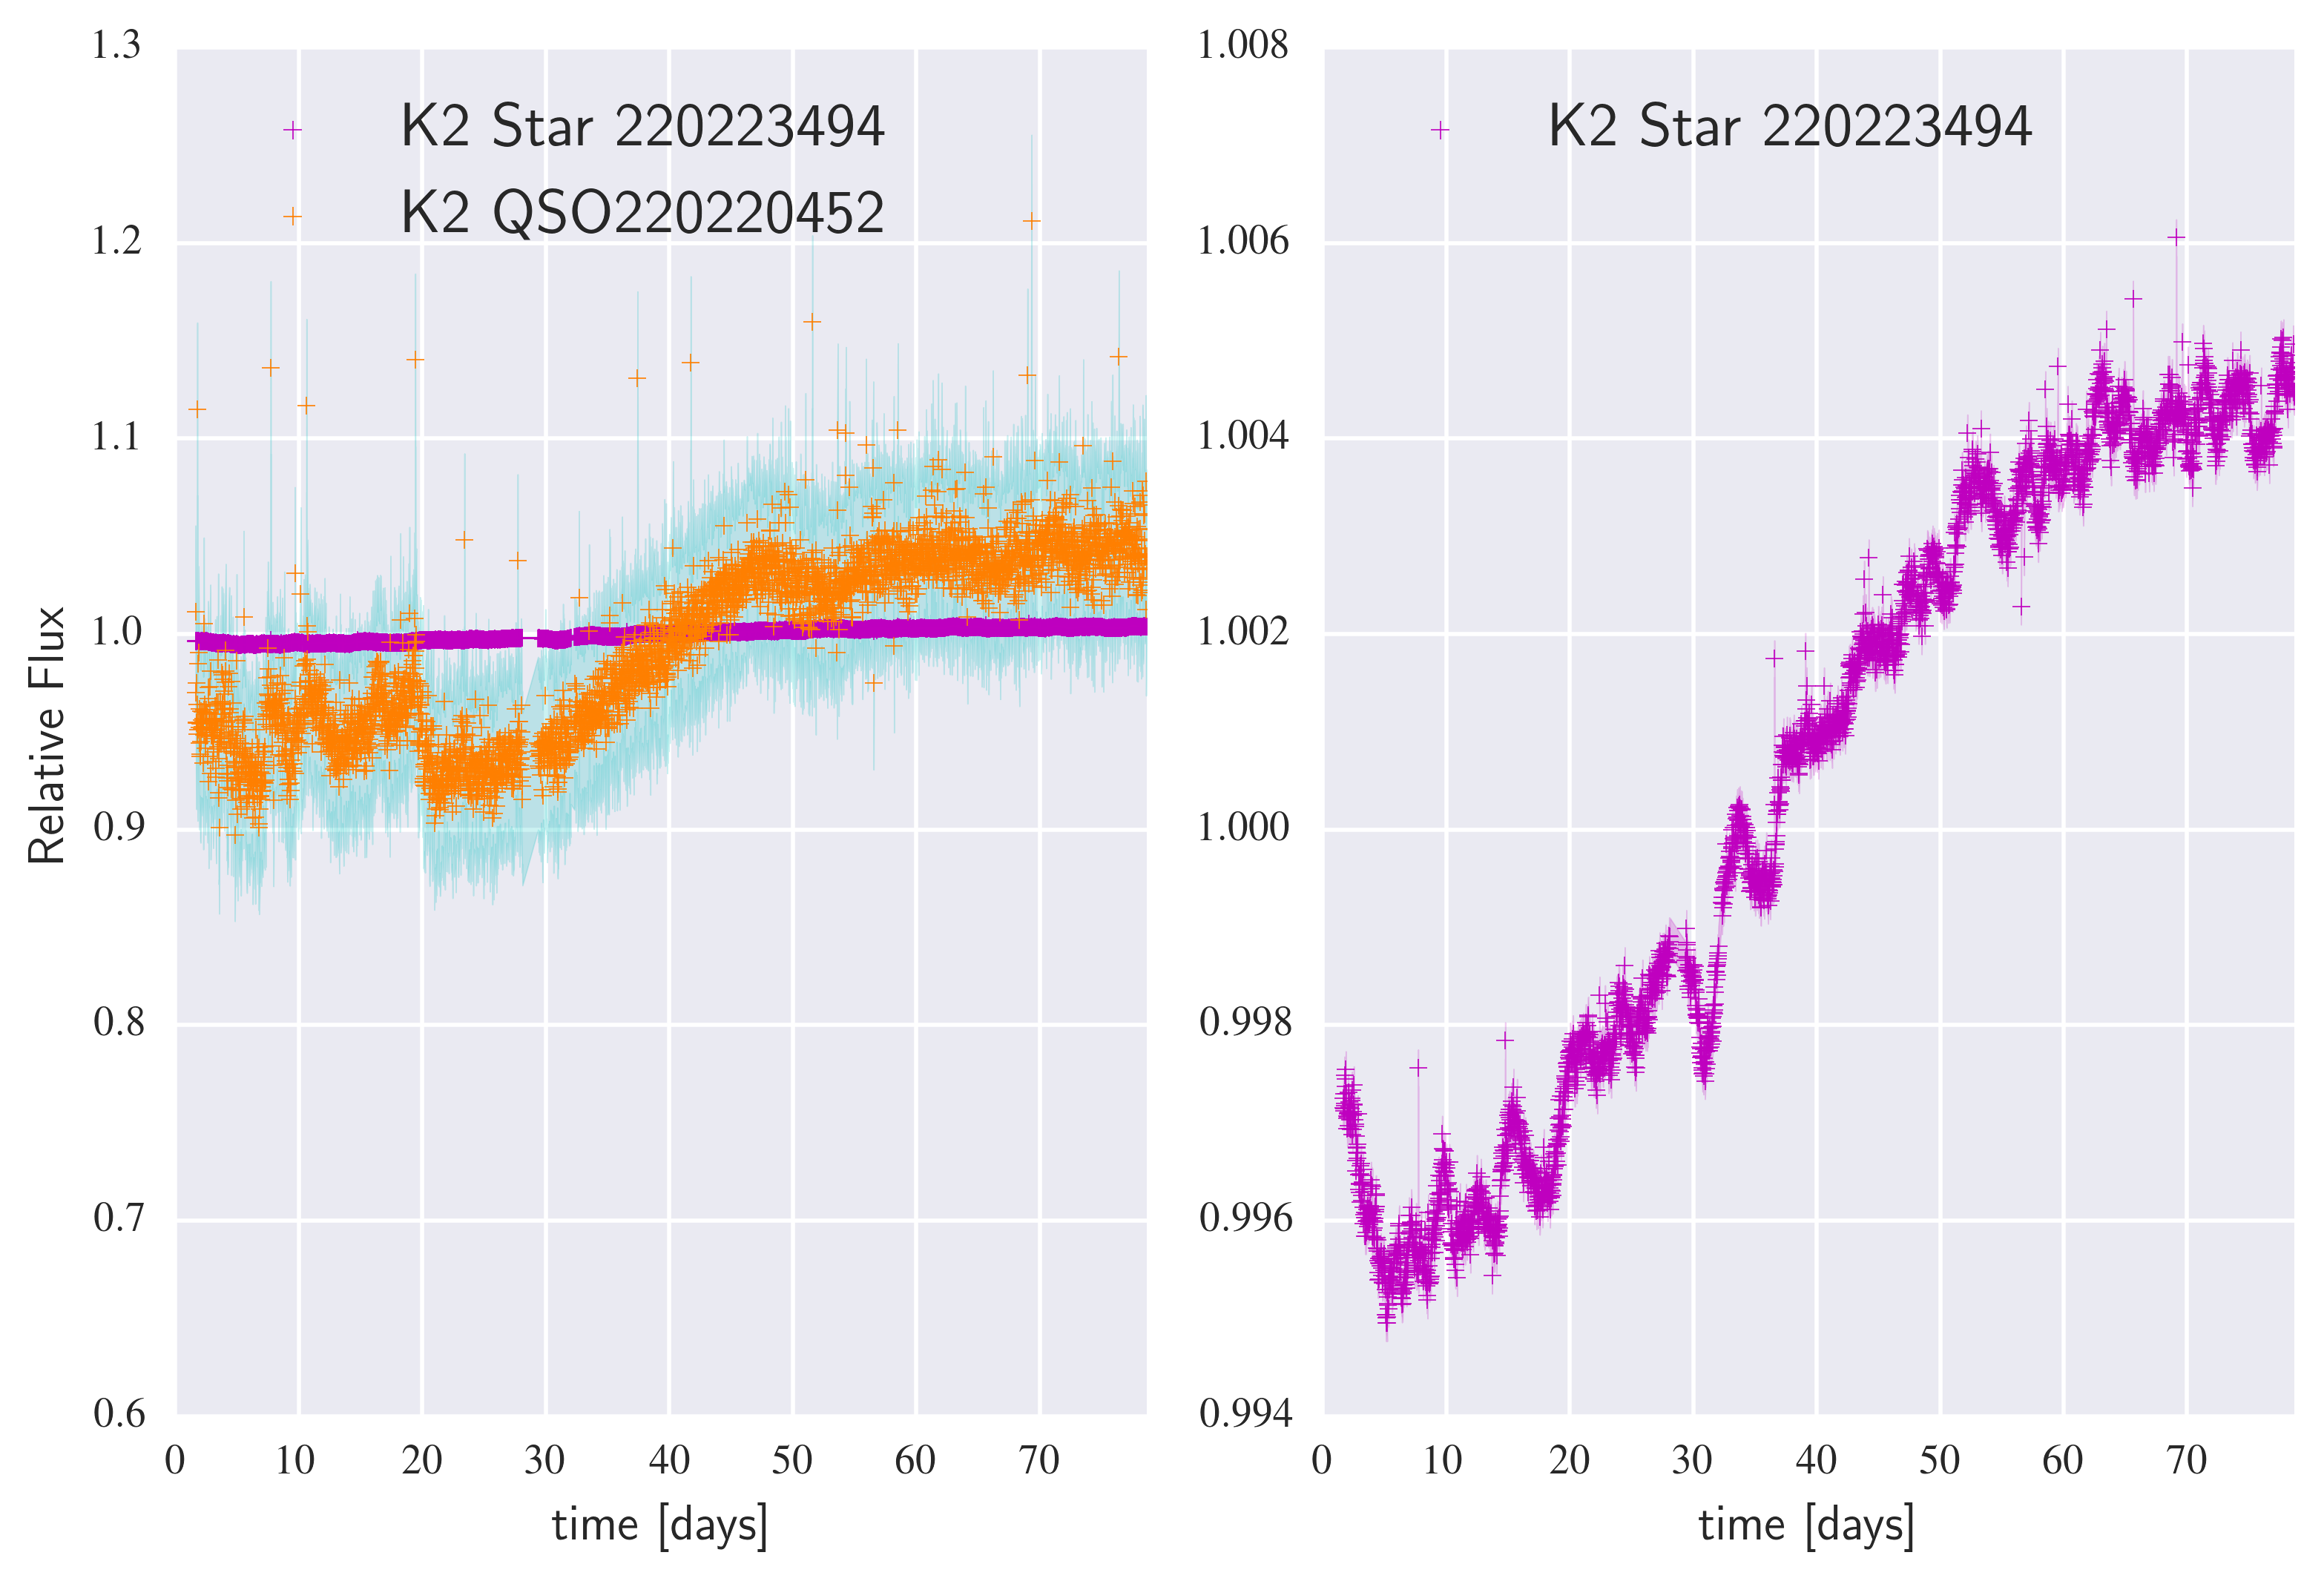
\includegraphics[width=\columnwidth]{220220452NearestNeighbor.png}
 	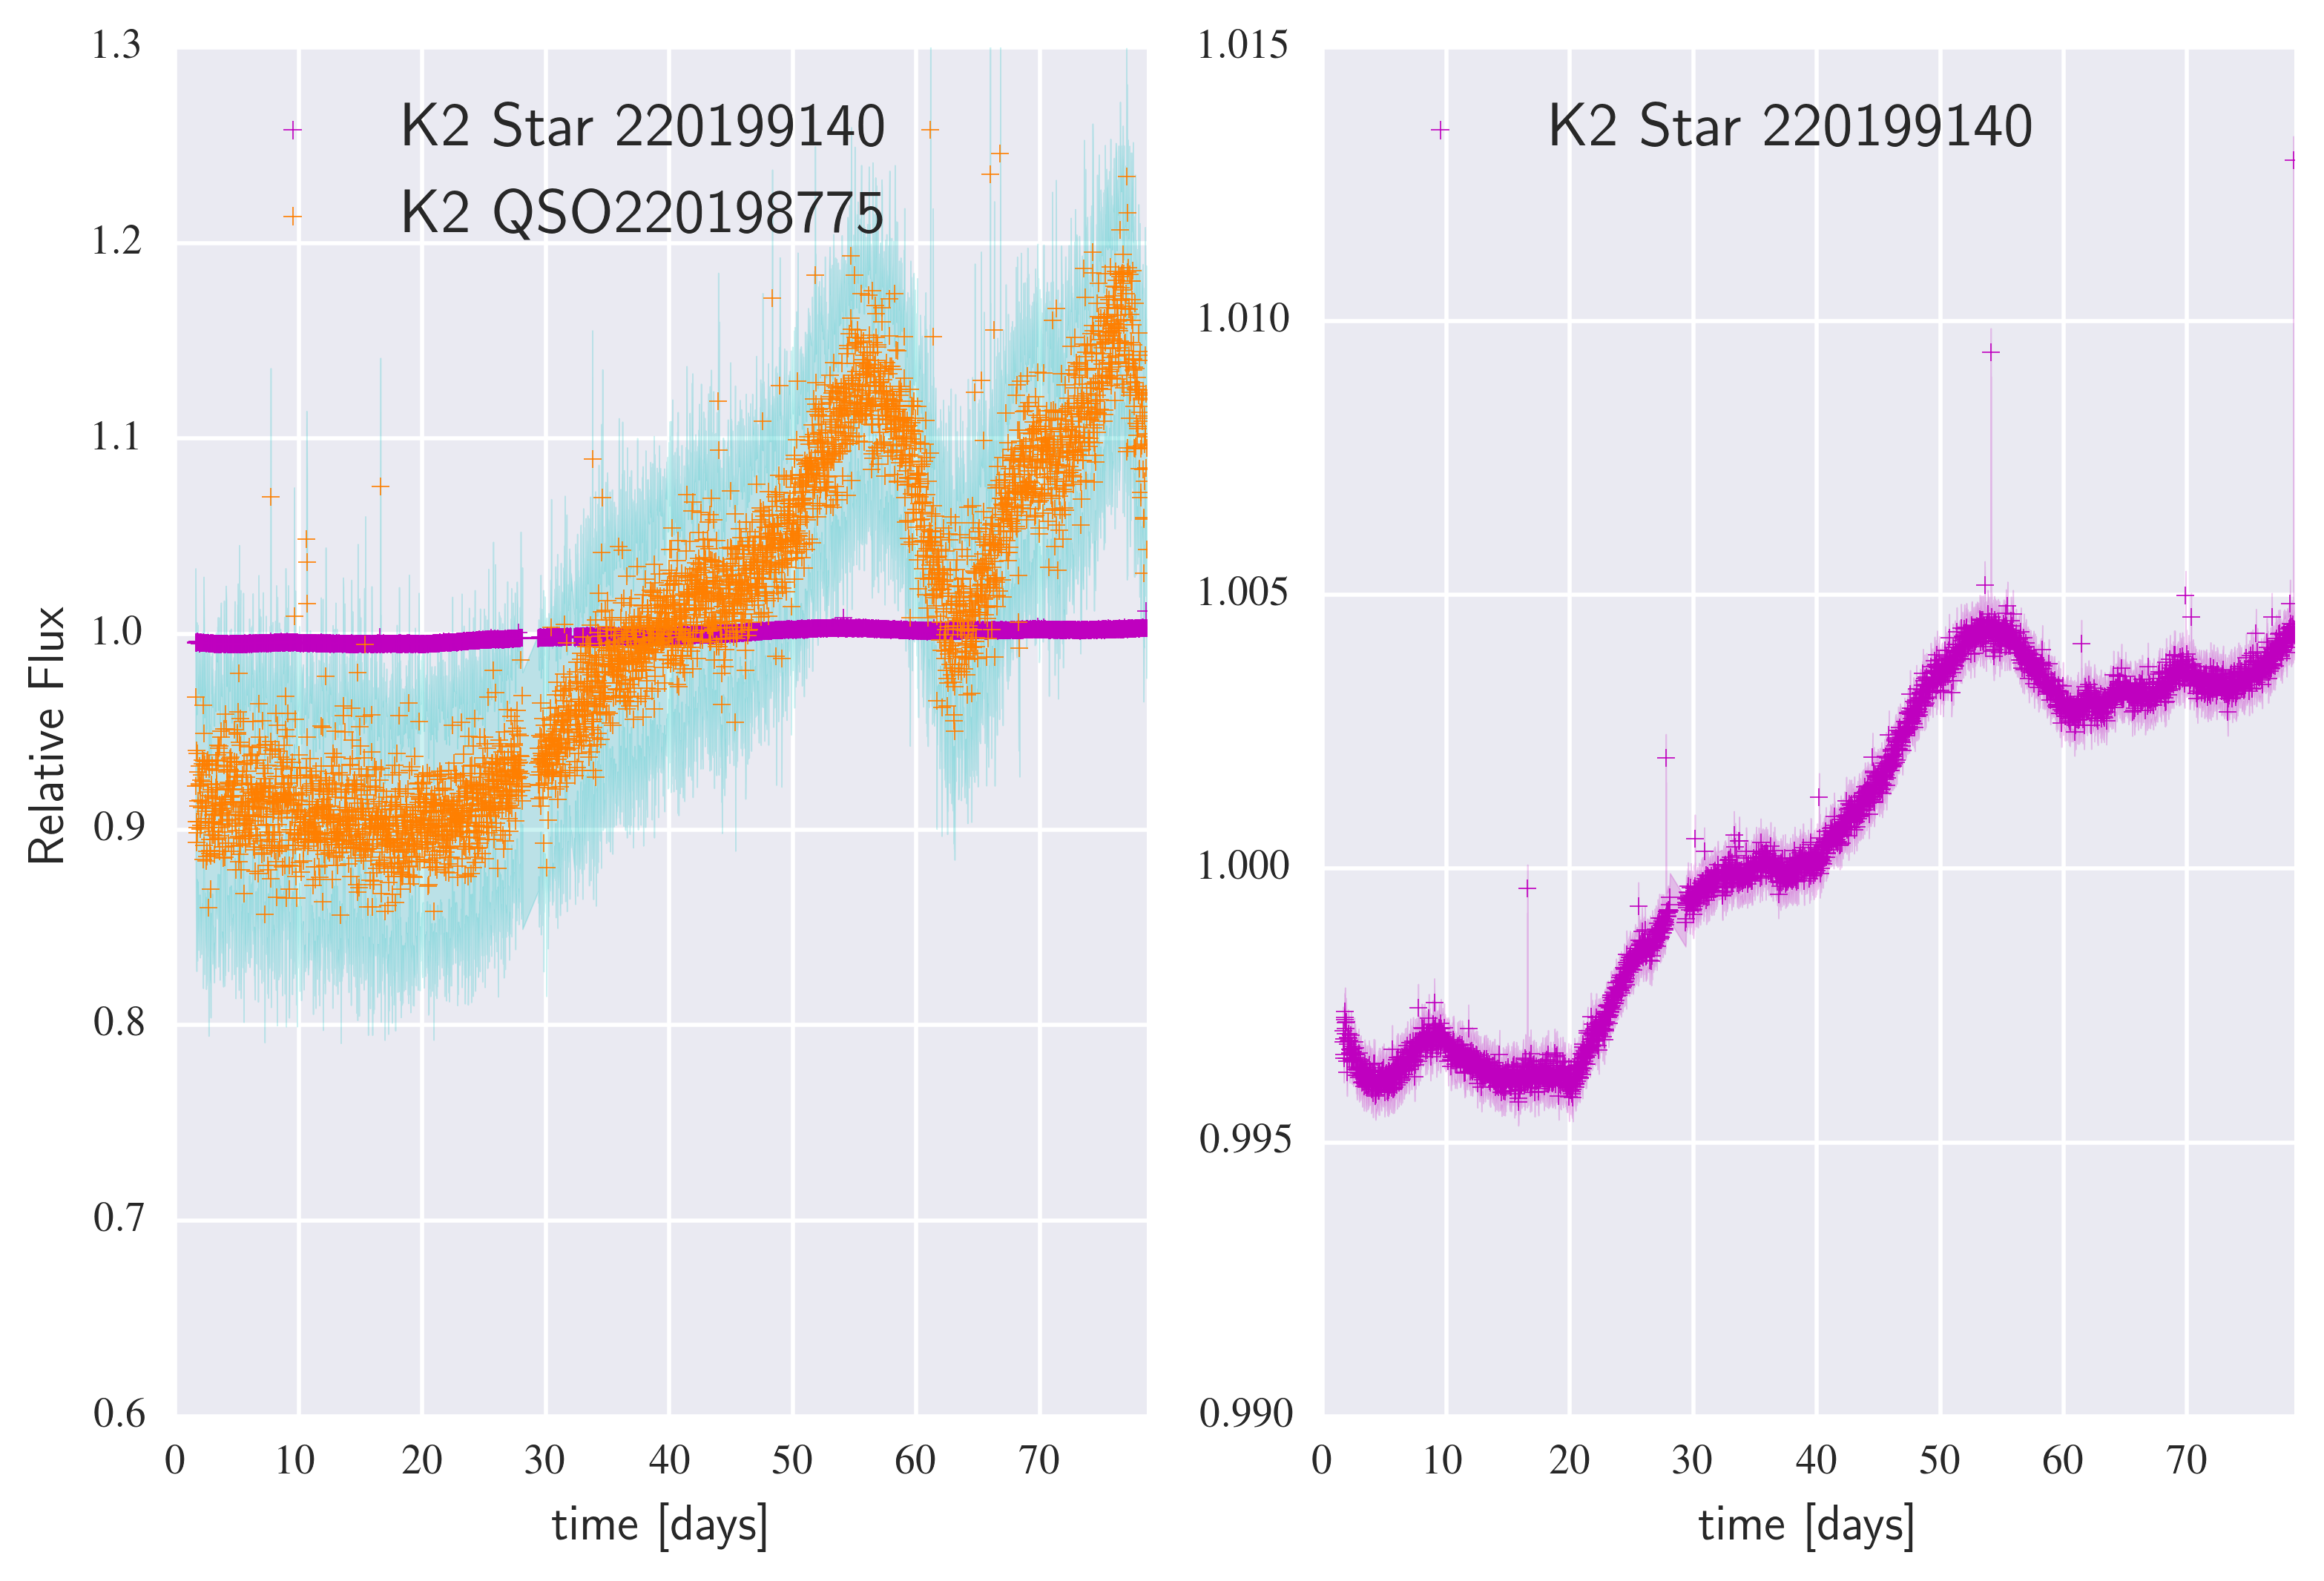
\includegraphics[width=\columnwidth]{220198775NearestNeighbor.png}
 	\includegraphics[width=\columnwidth]{220209831NearestNeighbor.png}
        	%	\includegraphics[width=\columnwidth]{220186429ExtendedLC.png}
        	\caption{}
        	\label{fig:example_figure}
        \end{figure}   
        	        	
        	        	
        	   \begin{figure}
        		% To include a figure from a file named example.*
        		% Allowable file formats are eps or ps if compiling using latex
        		% or pdf, png, jpg if compiling using pdflatex
 	\includegraphics[width=\columnwidth]{220170097NearestNeighbor.png}
 	\includegraphics[width=\columnwidth]{220221035NearestNeighbor.png}
 	\includegraphics[width=\columnwidth]{220192831NearestNeighbor.png}
        		\caption{}
        		\label{fig:example_figure}
        		\end{figure}          
        	
        	\begin{figure}
        	% To include a figure from a file named example.*
        	% Allowable file formats are eps or ps if compiling using latex
        	% or pdf, png, jpg if compiling using pdflatex
 	\includegraphics[width=\columnwidth]{220235253NearestNeighbor.png}
 	\includegraphics[width=\columnwidth]{220192000NearestNeighbor.png}
 	%\includegraphics[width=\columnwidth]{220186429NearestNeighbor.png}
        	\caption{}
        	\label{fig:example_figure}
        	\end{figure}    
        	
         
\end{document}
